% Guardar este .tex en la carpeta existente Downloads/build.
% !TeX encoding = UTF-8
% ARCHIVO AUTONOMO: todos los graficos son vectoriales (TikZ/PGFPlots).
% Usar la misma receta que para mincer_pooled_matematica.tex.
% No fuerza el motor ni la ruta de salida; no requiere shell-escape.
% Paquetes estandar de MiKTeX. Si falta alguno, habilitar su instalacion.
% El idioma espanol se activa si babel-spanish esta instalado.
\documentclass[11pt,a4paper]{article}
\usepackage[utf8]{inputenc}
\usepackage[T1]{fontenc}
\usepackage{lmodern}
\IfFileExists{spanish.ldf}{\usepackage[spanish,es-nodecimaldot,es-noquoting]{babel}}{}
\usepackage[a4paper,margin=1.8cm,headheight=15pt]{geometry}
\usepackage{amsmath,amssymb,amsthm,mathtools,bm}
\usepackage{microtype,booktabs,array,longtable,multicol,enumitem}
\usepackage[dvipsnames]{xcolor}
\usepackage{tikz,pgfplots,tikz-3dplot}
\usetikzlibrary{arrows.meta,calc,angles,quotes,positioning,patterns,babel}
\usepgfplotslibrary{fillbetween,groupplots}
\pgfplotsset{compat=1.18}
\usepackage[most]{tcolorbox}
\usepackage{float,caption,fancyhdr}
\usepackage[colorlinks=true,linkcolor=MidnightBlue,urlcolor=MidnightBlue]{hyperref}
\hypersetup{pdftitle={Datos de panel: pooled, efectos fijos, aleatorios e inferencia},pdfauthor={Tratado de estudio}}
\pdfstringdefDisableCommands{\def\ell{l}\def\infty{infinito}\def\to{ a }\def\norm#1{norma(#1)}\def\R{R}\def\N{N}}
\definecolor{azul}{RGB}{21,64,112}
\definecolor{celeste}{RGB}{235,244,252}
\definecolor{rojo}{RGB}{181,58,58}
\definecolor{verde}{RGB}{27,119,94}
\definecolor{gris}{RGB}{83,94,108}
\pagestyle{fancy}\fancyhf{}
\fancyhead[L]{\small\color{azul}Datos de panel: teoría y problemas}
\fancyhead[R]{\small\color{gris}Pooled, FE, RE, IV y dinámica}
\fancyfoot[C]{\small\thepage}
\setlength{\parindent}{0pt}\setlength{\parskip}{4pt}
\setlength{\abovedisplayskip}{6pt}\setlength{\belowdisplayskip}{6pt}
\setlength{\abovedisplayshortskip}{4pt}\setlength{\belowdisplayshortskip}{4pt}
\setlist{nosep,leftmargin=*}
\allowdisplaybreaks[2]
\emergencystretch=2em
\captionsetup{font=small,labelfont=bf,skip=5pt}
\renewcommand{\contentsname}{Índice}
\renewcommand{\figurename}{Figura}
\renewcommand{\tablename}{Cuadro}
\newcommand{\R}{\mathbb R}
\newcommand{\N}{\mathbb N}
\newcommand{\E}{\mathbb E}
\newcommand{\Prob}{\mathbb P}
\newcommand{\ind}{\mathbf 1}
\newcommand{\dd}{\,\mathrm d}
\newcommand{\T}{^{\mathsf T}}
\newcommand{\norm}[1]{\left\lVert #1\right\rVert}
\newcommand{\abs}[1]{\left\lvert #1\right\rvert}
\newcommand{\ip}[2]{\left\langle #1,#2\right\rangle}
\DeclareMathOperator{\Var}{Var}
\DeclareMathOperator{\Cov}{Cov}
\DeclareMathOperator{\Corr}{Corr}
\DeclareMathOperator{\spanop}{span}
\DeclareMathOperator{\esssup}{ess\,sup}
\DeclareMathOperator*{\argmin}{arg\,min}
\DeclareMathOperator{\sign}{sign}
\DeclareMathOperator{\tr}{tr}
\newtcolorbox{idea}[1][]{enhanced,breakable,colback=celeste,colframe=azul,boxrule=.5pt,arc=1mm,left=6pt,right=6pt,top=4pt,bottom=4pt,title={#1},fonttitle=\bfseries}
\newtcolorbox{ejemplo}[1][]{enhanced,breakable,colback=white,colframe=verde,boxrule=.5pt,arc=1mm,left=6pt,right=6pt,top=4pt,bottom=4pt,title={#1},fonttitle=\bfseries}
\newtcolorbox{cuidado}[1][]{enhanced,breakable,colback=red!2,colframe=rojo,boxrule=.5pt,arc=1mm,left=6pt,right=6pt,top=4pt,bottom=4pt,title={#1},fonttitle=\bfseries}
\newenvironment{deduccion}{\par\textbf{Deducción.}\ }{\hfill$\square$\par}
\pgfplotsset{base/.style={axis lines=middle,grid=both,minor tick num=1,grid style={gray!12},major grid style={gray!23},tick label style={font=\scriptsize},label style={font=\small},legend style={font=\scriptsize,draw=none,fill=white},samples=140},curva/.style={very thick,azul}}
\tikzset{vec/.style={-{Latex[length=2.6mm]},very thick,azul},vecrojo/.style={-{Latex[length=2.6mm]},very thick,rojo},vecverde/.style={-{Latex[length=2.6mm]},very thick,verde},eje/.style={-{Latex[length=1.8mm]},gray}}


\usepackage{listings,needspace}
\lstset{basicstyle=\ttfamily\footnotesize,breaklines=true,frame=single,rulecolor=\color{azul!40},backgroundcolor=\color{celeste!35},columns=fullflexible,keepspaces=true,showstringspaces=false}
\DeclareMathOperator{\rank}{rank}
\DeclareMathOperator{\diag}{diag}
\DeclareMathOperator{\kerop}{ker}
\DeclareMathOperator{\range}{Im}
\DeclareMathOperator*{\argmax}{arg\,max}
\newcommand{\Id}{I}
\newcommand{\F}{_{\mathrm F}}
\newcommand{\ones}{\mathbf 1}
\newcommand{\Sph}{\mathbb S}
\newtheorem{teorema}{Teorema}[section]
\newtheorem{proposicion}[teorema]{Proposición}
\newtheorem{lema}[teorema]{Lema}
\theoremstyle{definition}
\newtheorem{definicion}[teorema]{Definición}
\newcommand{\parte}[1]{\par\bigskip\Needspace{8\baselineskip}\begin{center}{\Large\bfseries\color{azul}#1}\end{center}}
\renewcommand{\proofname}{Demostración}

\newcounter{problema}
\newenvironment{resuelto}[1]{\refstepcounter{problema}\par\medskip\Needspace{6\baselineskip}\textbf{Problema \theproblema. #1}\par}{\par\medskip}


\DeclareMathOperator{\plim}{plim}
\DeclareMathOperator{\vecop}{vec}
\DeclareMathOperator{\se}{se}
\newcommand{\eps}{\varepsilon}
\newcommand{\cX}{\mathcal X}
\newcommand{\cO}{\mathcal O}
\pgfplotsset{panelaxis/.style={axis lines=box,grid=major,minor tick num=0,grid style={gray!20},width=13.1cm,height=5.2cm,tick label style={font=\scriptsize},label style={font=\small},legend style={at={(0.5,-0.28)},anchor=north,legend columns=3,font=\scriptsize,draw=none,fill=white},samples=120}}
\begin{document}
\begin{center}
{\Huge\bfseries\color{azul}Datos de panel}\\[6pt]
{\Large Matemática, geometría, inferencia y problemas resueltos}\\[5pt]
{\large Pooled, efectos fijos, efectos aleatorios, IV, GMM y causalidad}\\[4pt]
\textit{Una clase extensa desde los escalares hasta los paneles de gran dimensión}
\end{center}
\begin{idea}[La ecuación central y las preguntas que exige]
\[
y_{it}=a_i+\lambda_t+x_{it}^{\mathsf T}\beta+\eps_{it}.
\]
$i$ identifica a una entidad y $t$ al tiempo. $a_i$ representa diferencias permanentes; $\lambda_t$, choques comunes; $x_{it}$, variables observadas. Queremos saber cuándo podemos identificar $\beta$, cómo estimarlo y cómo calcular la esperanza, la varianza y la covarianza de lo que estimamos.
\end{idea}
\textbf{Lectura desde cero.} Primero construimos una observación, un vector, una matriz y una esperanza. Después deducimos MCO, pooled, between, FE y RE. Desarrollamos inferencia, instrumentos, dinámica y diferencias en diferencias. Cada capítulo conecta la fórmula con sus condiciones y con lo que puede fallar. Los problemas contienen datos sintéticos: sus números son ejercicios reproducibles, no estimaciones de una encuesta real.

\textbf{Notación que no oculta los cálculos.} En las pruebas generales usamos sumatorias y matrices para permitir cualquier dimensión. En los ejemplos pequeños desplegamos las filas, los productos cruzados, las inversas y los resultados. La notación compacta se introduce después de mostrar qué operación representa. Una identidad exacta lleva $=$; un número redondeado lleva $\approx$.

\textbf{Propiedades exactas y aproximadas.} Una matriz de covarianza condicional con diseño fijo no equivale automáticamente a una varianza incondicional. Una fórmula gaussiana de muestra finita no equivale a una aproximación robusta de muchos conglomerados. Identificamos el régimen asintótico antes de usar límites. FE y RE son modelos con condiciones diferentes; un contraste no reemplaza el conocimiento del diseño.

\textbf{Material de estudio.} 59 problemas resueltos, 22 figuras vectoriales, talleres numéricos completos y un laboratorio reproducible.\par
\textbf{Extensión compilada.} \pageref{ultima-pagina} páginas. Las figuras son vectoriales y están integradas en este mismo archivo. Los ejercicios numéricos incluyen coeficientes, residuos, productos matriciales y medidas de incertidumbre.

\textbf{Tu receta y tu carpeta.} Guarda únicamente este fuente en tu carpeta existente \texttt{Downloads/build}, junto a tus otros archivos \texttt{.tex}. Usa tu receta habitual de pdfLaTeX. El modelo de compilación es el archivo salarial que ya funciona. Tres pasadas actualizan índice y referencias. No se fuerza motor ni directorio de salida, no se crea una carpeta \texttt{build/build}, no se borra ningún archivo y no se requiere \texttt{shell-escape}.

\textbf{Convenciones.} $G$ es el número de entidades; $T_i$, sus períodos observados; $n=\sum_{i=1}^G T_i$, el número de filas. $K$ cuenta pendientes; $p$ cuenta columnas de un diseño concreto, incluyendo las constantes que correspondan. $\T$ indica transposición; $\ones_m$ es el vector de $m$ unos; $I_m$ es la identidad. $\Var(V)$ y $\Cov(V,W)$ son matrices cuando sus argumentos son vectores. Las covarianzas estimadas llevan sombrero.
\setcounter{tocdepth}{1}
\section*{Índice de la ruta de aprendizaje}
\begin{multicols}{2}\footnotesize\setlength{\parskip}{0pt}
\makeatletter
\renewcommand*\l@section[2]{\@dottedtocline{1}{0pt}{2.5em}{#1}{#2}}
\@starttoc{toc}
\makeatother
\end{multicols}

% MODULO 01_estructuras.tex
\parte{I. Qué es un panel y de qué están hechas sus ecuaciones}
\section{Una fila, una persona y una fecha son objetos distintos}
Una observación es una colección de valores medidos en una unidad y un momento. Si seguimos a una persona durante tres años, hay tres filas y una persona. Si encuestamos a tres personas diferentes, una cada año, también hay tres filas; no existe una trayectoria individual. Esa diferencia determina qué variación puede eliminar un efecto fijo.

Sea $\cO=\{(i,t):\text{el par entidad--tiempo fue observado}\}$. Un panel es balanceado cuando cada entidad aparece en los mismos $T$ períodos. Entonces $\cO=\{1,\ldots,G\}\times\{1,\ldots,T\}$ y $n=GT$. Es desbalanceado si algunas parejas faltan. Es rotativo si el diseño renueva parte de las entidades. Un corte transversal observa muchas unidades en una fecha; una serie temporal sigue una unidad; cortes repetidos observan muestras nuevas en diferentes fechas. Una etiqueta de hogar que cambia de significado no crea continuidad.

\begin{ejemplo}[Panel sintético mínimo]
\begin{center}
\begin{tabular}{rrrr}
\toprule
Entidad $i$ & Tiempo $t$ & $x_{it}$ & $y_{it}$\\
\midrule
1&1&1&3\\1&2&2&5\\1&3&3&7\\
2&1&2&8\\2&2&3&10\\2&3&4&12\\
\bottomrule
\end{tabular}
\end{center}
La primera trayectoria satisface $y=1+2x$; la segunda, $y=4+2x$. Hay $G=2$, $T=3$, $n=6$. La pendiente dentro de cada entidad es $2$. La diferencia de interceptos es $3$. Mezclar ambos grupos en una sola recta introduce otra fuente de variación.
\end{ejemplo}
Una clave de panel exige unicidad: para cada par $(i,t)$ debe haber como máximo una fila, salvo que se defina otra unidad, como persona--empleo--mes. Si aparecen dos empleos de una persona en un mes, ni promediarlos ni conservar ambos es una operación inocua: cambia la unidad, el peso y el resultado que se modela.



% PANELFIG 1
\begin{figure}[htbp]\centering
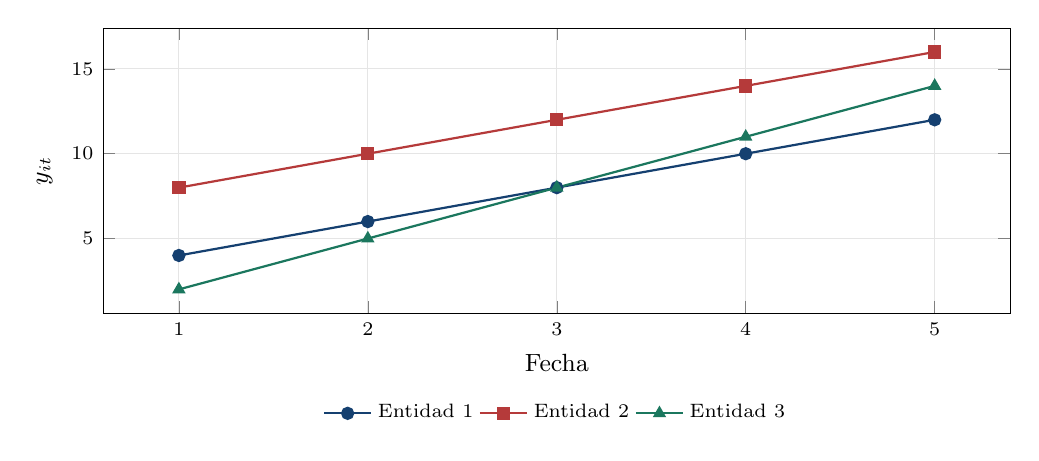
\begin{tikzpicture}
\begin{axis}[panelaxis,xlabel={Fecha},ylabel={$y_{it}$},xtick={1,2,3,4,5}]
\addplot[azul,thick,mark=*] coordinates {(1,4) (2,6) (3,8) (4,10) (5,12)};
\addlegendentry{Entidad 1}
\addplot[rojo,thick,mark=square*] coordinates {(1,8) (2,10) (3,12) (4,14) (5,16)};
\addlegendentry{Entidad 2}
\addplot[verde,thick,mark=triangle*] coordinates {(1,2) (2,5) (3,8) (4,11) (5,14)};
\addlegendentry{Entidad 3}
\end{axis}
\end{tikzpicture}
\caption{Tres trayectorias sintéticas. Observar varias fechas de la misma entidad permite estudiar cambios; las diferencias de nivel y de pendiente son objetos separados.}\label{fig:panel-1}
\end{figure}
% FIN PANELFIG
\section{Escalares, vectores y productos interiores}
Un escalar es un número. Un vector columna de $K$ características es
\[
x_{it}=\begin{pmatrix}x_{it,1}\\x_{it,2}\\\vdots\\x_{it,K}\end{pmatrix},
\qquad
\beta=\begin{pmatrix}\beta_1\\\beta_2\\\vdots\\\beta_K\end{pmatrix}.
\]
Su producto interior es un escalar:
\[
x_{it}\T\beta=\sum_{k=1}^K x_{it,k}\beta_k.
\]
Con educación $12$, experiencia $5$ y experiencia al cuadrado $25$,
\[
\begin{pmatrix}12&5&25\end{pmatrix}
\begin{pmatrix}0.08\\0.04\\-0.001\end{pmatrix}
=12(0.08)+5(0.04)+25(-0.001)=1.135.
\]
El cuadrado de una variable es una nueva columna; el cuadrado de su coeficiente no participa en esta especificación. El producto de un indicador con una variable también es una columna nueva.

Para $v,w\in\R^m$, la norma euclídea es $\norm v=(\sum_{j=1}^m v_j^2)^{1/2}$ y la distancia es $\norm{v-w}$. Dos vectores son ortogonales si $v\T w=0$. La desigualdad de Cauchy--Schwarz,
\[
|v\T w|\le\norm v\,\norm w,
\]
se demuestra expandiendo $\norm{v-cw}^2\ge0$ y eligiendo $c=(v\T w)/(w\T w)$ cuando $w\ne0$. La correlación y muchas cotas de error usan esta misma geometría.

Una matriz $A\in\R^{m\times p}$ contiene $m$ filas y $p$ columnas. El elemento $(j,k)$ es $A_{jk}$. Si $b\in\R^p$, entonces $(Ab)_j=\sum_{k=1}^p A_{jk}b_k$. La transpuesta intercambia filas y columnas. La identidad $I_p$ deja cualquier vector inalterado: $I_pb=b$. El rango es el número de columnas linealmente independientes; un coeficiente solo se identifica de forma única cuando ninguna columna necesaria es combinación de las demás.

\section{Apilar un panel sin cambiar su contenido}
Ordenemos primero por entidad y después por tiempo. En el panel anterior,
\[
y=\begin{pmatrix}3\\5\\7\\8\\10\\12\end{pmatrix},\quad
X=\begin{pmatrix}1\\2\\3\\2\\3\\4\end{pmatrix},\quad
D=\begin{pmatrix}
1&0\\1&0\\1&0\\0&1\\0&1\\0&1
\end{pmatrix},\quad
a=\begin{pmatrix}1\\4\end{pmatrix}.
\]
Entonces $Da$ repite el intercepto de cada entidad:
\[
Da=\begin{pmatrix}1\\1\\1\\4\\4\\4\end{pmatrix},\qquad
X\beta=\begin{pmatrix}2\\4\\6\\4\\6\\8\end{pmatrix},\qquad
y=Da+X\beta.
\]
La matriz $D$ es de incidencia: $D_{(i,t),j}=1$ si $j=i$ y $0$ en otro caso. Con errores, la ecuación es $y=Da+X\beta+\eps$. Aquí $y,\eps\in\R^n$, $D\in\R^{n\times G}$, $X\in\R^{n\times K}$.

Si se agrega una constante global y las $G$ columnas de $D$, surge dependencia porque $D\ones_G=\ones_n$. Para estimar se elimina una dummy o se impone una restricción como $\sum_i a_i=0$ junto con un intercepto global. Ambas parametrizaciones pueden producir exactamente los mismos valores ajustados; los interceptos reportados tienen interpretaciones distintas.

\section{El producto de Kronecker: repetir estructuras}
Para una matriz $A=(a_{jk})$ y otra $B$, $A\otimes B$ reemplaza cada entrada $a_{jk}$ por el bloque $a_{jk}B$. Con panel balanceado,
\[
D=I_G\otimes\ones_T,\qquad D\T D=T I_G.
\]
Por ejemplo,
\[
I_2\otimes\begin{pmatrix}1\\1\end{pmatrix}
=
\begin{pmatrix}1&0\\1&0\\0&1\\0&1\end{pmatrix}.
\]
Las propiedades $(A\otimes B)\T=A\T\otimes B\T$ y
$(A\otimes B)(C\otimes E)=(AC)\otimes(BE)$ se obtienen multiplicando bloques, cuando las dimensiones permiten los productos. También
$\tr(A\otimes B)=\tr(A)\tr(B)$ para matrices cuadradas.

Una permutación del orden de filas es una matriz $P$ con exactamente un $1$ por fila y columna. Satisface $P\T P=I$. Reordenar todos los objetos consistentemente transforma $(y,X,\Omega)$ en $(Py,PX,P\Omega P\T)$ y no cambia MCO o GLS. Reordenar únicamente $y$ sí destruye el emparejamiento y cambia la regresión.

\section{Medias, desviaciones y una identidad fundamental}
Definimos $\bar x_i=T_i^{-1}\sum_{t\in\mathcal T_i}x_{it}$, donde $\mathcal T_i$ es el conjunto de tiempos observados de $i$. La media global por fila es
\[
\bar x=\frac1n\sum_{i=1}^G\sum_{t\in\mathcal T_i}x_{it}
=\frac1n\sum_{i=1}^G T_i\bar x_i.
\]
En un panel desbalanceado no coincide necesariamente con $G^{-1}\sum_i\bar x_i$.
La identidad
\[
x_{it}-\bar x=(x_{it}-\bar x_i)+(\bar x_i-\bar x)
\]
separa variación dentro y entre entidades. Al multiplicar y sumar,
\[
\begin{aligned}
\sum_i\sum_t(x_{it}-\bar x)^2
&=\sum_i\sum_t(x_{it}-\bar x_i)^2
+\sum_i T_i(\bar x_i-\bar x)^2\\
&\quad+2\sum_i(\bar x_i-\bar x)
\underbrace{\sum_t(x_{it}-\bar x_i)}_{0}.
\end{aligned}
\]
Esta es una descomposición exacta, no un supuesto probabilístico. Para dos variables se obtiene análogamente
\[
\sum_i\sum_t(x_{it}-\bar x)(y_{it}-\bar y)
=\sum_i\sum_t(x_{it}-\bar x_i)(y_{it}-\bar y_i)
+\sum_iT_i(\bar x_i-\bar x)(\bar y_i-\bar y).
\]
La pendiente pooled puede cambiar porque combina esos dos productos cruzados.

\begin{resuelto}{Contar y promediar en un panel desbalanceado}
La entidad 1 tiene $x=(1,3)$; la entidad 2, $x=(2,4,6)$.
Entonces $T_1=2$, $T_2=3$, $n=5$,
\[
\bar x_1=(1+3)/2=2,\qquad
\bar x_2=(2+4+6)/3=4,\qquad
\bar x=(1+3+2+4+6)/5=16/5.
\]
La media de medias sin ponderar es $(2+4)/2=3$, mientras que
$(2\cdot2+3\cdot4)/5=16/5$. La suma de cuadrados dentro es
$(1-2)^2+(3-2)^2+(2-4)^2+(4-4)^2+(6-4)^2=10$.
La suma entre es $2(2-16/5)^2+3(4-16/5)^2=24/5$.
La suma total es $74/5=10+24/5$. Un panel con más filas de una entidad da mayor peso a su media en la descomposición por observaciones.
\end{resuelto}

\section{Distancias ponderadas y el motivo de GLS}
Si $\Omega$ es simétrica y definida positiva, $v\T\Omega^{-1}v>0$ para todo $v\ne0$. La distancia de Mahalanobis es
\[
d_\Omega(y,m)=\sqrt{(y-m)\T\Omega^{-1}(y-m)}.
\]
Si $\Omega=\diag(1,4)$, entonces $d_\Omega^2=(y_1-m_1)^2+(y_2-m_2)^2/4$.
Una desviación de dos unidades en el segundo componente pesa como una desviación de una unidad en el primero. La matriz de covarianza define qué direcciones son ruidosas; GLS reduce su peso relativo.

Una factorización $\Omega=LL\T$, con $L$ triangular invertible, transforma el error en $L^{-1}\eps$, cuya covarianza es la identidad. Por eso minimizar una distancia de Mahalanobis equivale a aplicar MCO sobre datos blanqueados. No necesitamos normalidad para esta identidad algebraica.

\section{Curiosidad: aumentar filas no siempre aumenta información}
Con $T$ repeticiones perfectamente correlacionadas de una entidad, las $T$ filas contienen una única realización aleatoria. Con errores de correlación intraclase $\rho$, varianza $\sigma_v^2$ y pesos iguales,
\[
\Var(\bar v)=\frac{\sigma_v^2}{T}\{1+(T-1)\rho\}.
\]
Para deducirla, sumamos $T$ varianzas y $T(T-1)$ covarianzas, y dividimos por $T^2$. Cuando $\rho=0$ se obtiene $\sigma_v^2/T$; cuando $\rho=1$, $\sigma_v^2$. Esta observación explica por qué una regresión con miles de filas pero pocos conglomerados puede tener poca precisión para variables constantes por grupo.



% PANELFIG 3
\begin{figure}[htbp]\centering
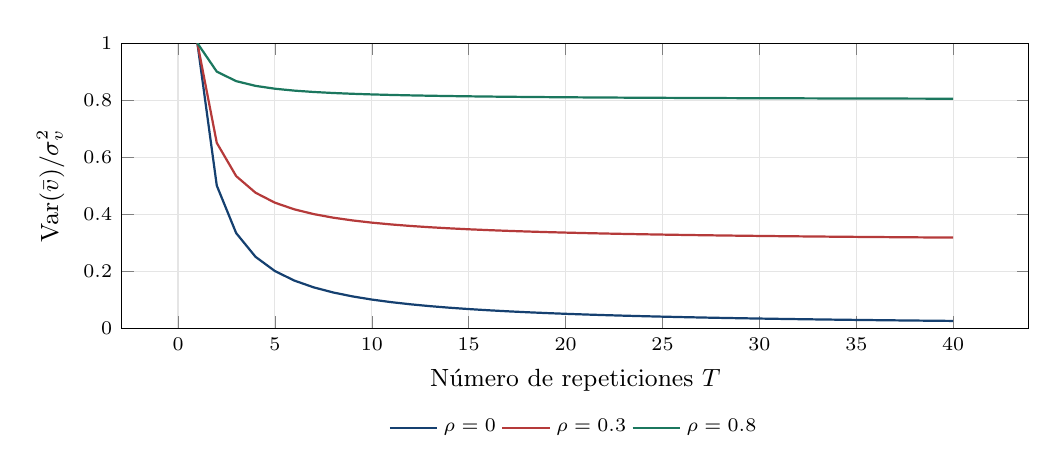
\begin{tikzpicture}
\begin{axis}[panelaxis,xlabel={Número de repeticiones $T$},ylabel={$\Var(\bar v)/\sigma_v^2$},ymin=0,ymax=1]
\addplot[azul,thick,no marks] coordinates {(1,1) (2,0.5) (3,0.333333333) (4,0.25) (5,0.2) (6,0.166666667) (7,0.142857143) (8,0.125) (9,0.111111111) (10,0.1) (11,0.0909090909) (12,0.0833333333) (13,0.0769230769) (14,0.0714285714) (15,0.0666666667) (16,0.0625) (17,0.0588235294) (18,0.0555555556) (19,0.0526315789) (20,0.05) (21,0.0476190476) (22,0.0454545455) (23,0.0434782609) (24,0.0416666667) (25,0.04) (26,0.0384615385) (27,0.037037037) (28,0.0357142857) (29,0.0344827586) (30,0.0333333333) (31,0.0322580645) (32,0.03125) (33,0.0303030303) (34,0.0294117647) (35,0.0285714286) (36,0.0277777778) (37,0.027027027) (38,0.0263157895) (39,0.0256410256) (40,0.025)};
\addlegendentry{$\rho=0$}
\addplot[rojo,thick,no marks] coordinates {(1,1) (2,0.65) (3,0.533333333) (4,0.475) (5,0.44) (6,0.416666667) (7,0.4) (8,0.3875) (9,0.377777778) (10,0.37) (11,0.363636364) (12,0.358333333) (13,0.353846154) (14,0.35) (15,0.346666667) (16,0.34375) (17,0.341176471) (18,0.338888889) (19,0.336842105) (20,0.335) (21,0.333333333) (22,0.331818182) (23,0.330434783) (24,0.329166667) (25,0.328) (26,0.326923077) (27,0.325925926) (28,0.325) (29,0.324137931) (30,0.323333333) (31,0.322580645) (32,0.321875) (33,0.321212121) (34,0.320588235) (35,0.32) (36,0.319444444) (37,0.318918919) (38,0.318421053) (39,0.317948718) (40,0.3175)};
\addlegendentry{$\rho=0.3$}
\addplot[verde,thick,no marks] coordinates {(1,1) (2,0.9) (3,0.866666667) (4,0.85) (5,0.84) (6,0.833333333) (7,0.828571429) (8,0.825) (9,0.822222222) (10,0.82) (11,0.818181818) (12,0.816666667) (13,0.815384615) (14,0.814285714) (15,0.813333333) (16,0.8125) (17,0.811764706) (18,0.811111111) (19,0.810526316) (20,0.81) (21,0.80952381) (22,0.809090909) (23,0.808695652) (24,0.808333333) (25,0.808) (26,0.807692308) (27,0.807407407) (28,0.807142857) (29,0.806896552) (30,0.806666667) (31,0.806451613) (32,0.80625) (33,0.806060606) (34,0.805882353) (35,0.805714286) (36,0.805555556) (37,0.805405405) (38,0.805263158) (39,0.805128205) (40,0.805)};
\addlegendentry{$\rho=0.8$}
\end{axis}
\end{tikzpicture}
\caption{Varianza de una media con correlación intraclase. Repetir mediciones correlacionadas reduce menos la incertidumbre que añadir realizaciones independientes.}\label{fig:panel-3}
\end{figure}
% FIN PANELFIG


% MODULO 02_probabilidad.tex
\parte{II. Probabilidad y momentos: qué significa la incertidumbre}
\section{Variables aleatorias y esperanza desde una suma}
Una variable aleatoria asigna un número a cada resultado de un experimento. Si $Y$ toma valores $y_1,\ldots,y_m$ con probabilidades $p_j$, entonces $p_j\ge0$, $\sum_jp_j=1$ y
\[
\E Y=\sum_{j=1}^m y_jp_j.
\]
Si tiene densidad $f$, $\E Y=\int_\R y f(y)\dd y$, siempre que $\int|y|f(y)\dd y<\infty$. La condición de integrabilidad es parte de la definición; no toda distribución tiene media. La linealidad da $\E(cY+dZ)=c\E Y+d\E Z$ sin requerir independencia.

La varianza es $\Var(Y)=\E[(Y-\E Y)^2]=\E(Y^2)-(\E Y)^2$, si el segundo momento es finito. La covarianza es
\[
\Cov(Y,Z)=\E[(Y-\E Y)(Z-\E Z)]
=\E(YZ)-\E Y\,\E Z.
\]
De la expansión de un cuadrado,
\[
\Var(cY+dZ)=c^2\Var(Y)+d^2\Var(Z)+2cd\Cov(Y,Z).
\]
Si $B$ es Bernoulli con $\Prob(B=1)=p$, $\E B=p$ y $\Var(B)=p(1-p)$ porque $B^2=B$. Si $Y=c+B$, sumar una constante cambia la media y deja la varianza intacta.

\section{Esperanza condicional y exogeneidad}
La esperanza condicional $\E(Y\mid X)$ es una función de $X$. En el caso discreto,
\[
\E(Y\mid X=x)=\sum_y y\,\Prob(Y=y\mid X=x).
\]
La ley de esperanzas iteradas dice $\E[\E(Y\mid X)]=\E Y$. La descomposición de varianza es
\[
\Var(Y)=\E[\Var(Y\mid X)]+\Var[\E(Y\mid X)].
\]
\begin{deduccion}
Escribimos $Y-\E Y=(Y-\E[Y\mid X])+(\E[Y\mid X]-\E Y)$.
El producto cruzado tiene esperanza cero porque, condicionado en $X$,
$\E[Y-\E(Y\mid X)\mid X]=0$. Los otros dos cuadrados dan los términos de la identidad.
\end{deduccion}
Una media condicional nula, $\E(u\mid X)=0$, implica $\E(Xu)=0$ cuando el producto es integrable. El recíproco no es general: puede haber una función no lineal de $X$ en $u$ que sea ortogonal a $X$.

En un panel estático distinguimos:
\[
\begin{array}{ll}
\text{Contemporánea:}&\E(\eps_{it}\mid x_{it},a_i)=0,\\
\text{Secuencial:}&\E(\eps_{it}\mid x_{i1},\ldots,x_{it},a_i)=0,\\
\text{Estricta:}&\E(\eps_{it}\mid x_{i1},\ldots,x_{iT_i},a_i)=0.
\end{array}
\]
La estricta prohíbe que un choque presente determine regresores futuros. Es la condición suficiente habitual para insesgadez condicional del estimador within en el modelo estático. La secuencial puede justificar instrumentos pasados, pero no la transformación within ordinaria sin más restricciones.

\begin{resuelto}{Un regresor que responde al choque anterior}
Sea $\eps_{it}$ independiente en el tiempo, media cero y varianza $\sigma^2$, y sea
$x_{it}=\eps_{i,t-1}$. Entonces $\E(x_{it}\eps_{it})=0$.
Sin embargo,
$\E(x_{i,t+1}\eps_{it})=\E(\eps_{it}^2)=\sigma^2$.
Al restar medias,
\[
\E[(x_{it}-\bar x_i)\eps_{it}]
=0-\frac1T\sum_{s=1}^T\E(x_{is}\eps_{it}).
\]
Para un período interior con $t+1\le T$, la suma incluye $\sigma^2$, por lo que el resultado es $-\sigma^2/T$. Una covarianza contemporánea nula no basta para FE.
\end{resuelto}

\section{Esperanzas y covarianzas de vectores}
Para $V=(V_1,\ldots,V_m)\T$, $\E V$ se calcula componente a componente. Su covarianza es
\[
\Var(V)=\E[(V-\E V)(V-\E V)\T],
\quad [\Var(V)]_{jk}=\Cov(V_j,V_k).
\]
Es simétrica porque $\Cov(V_j,V_k)=\Cov(V_k,V_j)$. Es semidefinida positiva porque
$c\T\Var(V)c=\Var(c\T V)\ge0$.
Para matrices deterministas $A,B$,
\[
\E(AV+b)=A\E V+b,\qquad
\Var(AV)=A\Var(V)A\T,\qquad
\Cov(AV,BW)=A\Cov(V,W)B\T.
\]
Estas fórmulas son el mecanismo de todas las covarianzas de estimadores lineales.

Con
\[
\Sigma=\begin{pmatrix}4&1\\1&9\end{pmatrix},
\qquad A=\begin{pmatrix}1&1\\1&-1\end{pmatrix},
\]
se obtiene
\[
A\Sigma=\begin{pmatrix}5&10\\3&-8\end{pmatrix},
\qquad
A\Sigma A\T=\begin{pmatrix}15&-5\\-5&11\end{pmatrix}.
\]
La suma tiene varianza $15$, la diferencia varianza $11$ y su covarianza es $-5$. Aunque las dos nuevas variables tienen signos simétricos, sus varianzas no tienen por qué coincidir.

\section{Normal univariada: densidad, momentos y simetría}
La normal $Y\sim N(\mu,\sigma^2)$, $\sigma>0$, tiene densidad
\[
f(y)=\frac1{\sqrt{2\pi}\sigma}
\exp\left[-\frac{(y-\mu)^2}{2\sigma^2}\right].
\]
La sustitución $z=(y-\mu)/\sigma$ reduce la integral a la normal estándar.
Para justificar la constante, sea $I=\int_\mathbb R e^{-z^2/2}\dd z$. Como el integrando es positivo, podemos multiplicar integrales y usar coordenadas polares en el plano:
\[
I^2=\int_{\mathbb R^2}e^{-(x^2+y^2)/2}\dd x\dd y
=\int_0^{2\pi}\int_0^\infty e^{-r^2/2}r\dd r\dd\theta=2\pi.
\]
La integral radial vale uno mediante $v=r^2/2$. Como $I>0$, $I=\sqrt{2\pi}$, de modo que la densidad estándar integra uno. El cambio de variables utiliza el Jacobiano polar $r$.

La simetría da $\E Z=0$. Integrando por partes y usando
$\varphi'(z)=-z\varphi(z)$,
\[
\E Z^2=\int_\R z^2\varphi(z)\dd z
=-[z\varphi(z)]_{-\infty}^\infty+\int_\R\varphi(z)\dd z=1.
\]
Así $\E Y=\mu$ y $\Var(Y)=\sigma^2$. La función generadora de momentos es
\[
\E(e^{sY})=\exp(\mu s+\sigma^2s^2/2).
\]
Se obtiene completando el cuadrado en $sy-(y-\mu)^2/(2\sigma^2)$; sus derivadas en cero producen los momentos.

La CDF $\Phi(z)=\int_{-\infty}^z\varphi(v)\dd v$ no requiere una expresión elemental para definir probabilidades. Bajo normalidad, una combinación lineal de errores sigue siendo normal. Esa propiedad da distribuciones exactas de coeficientes lineales; la consistencia de MCO no necesita normalidad.



% PANELFIG 5
\begin{figure}[htbp]\centering
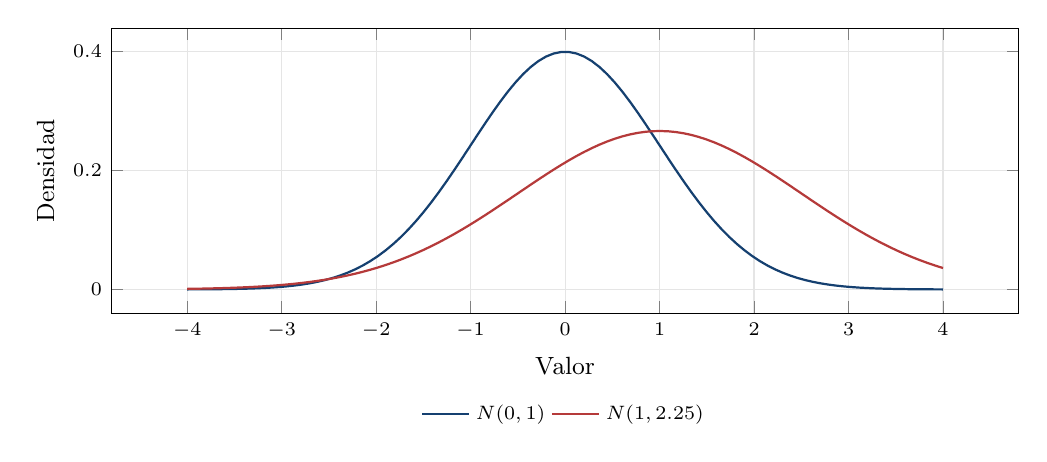
\begin{tikzpicture}
\begin{axis}[panelaxis,xlabel={Valor},ylabel={Densidad}]
\addplot[azul,thick,no marks] coordinates {(-4,0.000133830226) (-3.91919192,0.000184295302) (-3.83838384,0.000252138056) (-3.75757576,0.000342709873) (-3.67676768,0.000462784614) (-3.5959596,0.000620862299) (-3.51515152,0.000827514755) (-3.43434343,0.00109577221) (-3.35353535,0.00144154732) (-3.27272727,0.00188408981) (-3.19191919,0.00244646147) (-3.11111111,0.00315601632) (-3.03030303,0.00404486639) (-2.94949495,0.00515030799) (-2.86868687,0.00651517825) (-2.78787879,0.00818810653) (-2.70707071,0.0102236211) (-2.62626263,0.0126820683) (-2.54545455,0.0156292995) (-2.46464646,0.0191360817) (-2.38383838,0.0232771927) (-2.3030303,0.0281301641) (-2.22222222,0.033773651) (-2.14141414,0.0402854146) (-2.06060606,0.0477399263) (-1.97979798,0.0562056185) (-1.8989899,0.0657418315) (-1.81818182,0.0763955298) (-1.73737374,0.088197886) (-1.65656566,0.101160853) (-1.57575758,0.11527387) (-1.49494949,0.130500851) (-1.41414141,0.146777638) (-1.33333333,0.164010075) (-1.25252525,0.18207287) (-1.17171717,0.200809396) (-1.09090909,0.220032535) (-1.01010101,0.239526659) (-0.929292929,0.259050772) (-0.848484848,0.278342808) (-0.767676768,0.297125003) (-0.686868687,0.31511021) (-0.606060606,0.33200898) (-0.525252525,0.347537175) (-0.444444444,0.36142383) (-0.363636364,0.373418974) (-0.282828283,0.383301094) (-0.202020202,0.390883931) (-0.121212121,0.396022313) (-0.0404040404,0.398616779) (0.0404040404,0.398616779) (0.121212121,0.396022313) (0.202020202,0.390883931) (0.282828283,0.383301094) (0.363636364,0.373418974) (0.444444444,0.36142383) (0.525252525,0.347537175) (0.606060606,0.33200898) (0.686868687,0.31511021) (0.767676768,0.297125003) (0.848484848,0.278342808) (0.929292929,0.259050772) (1.01010101,0.239526659) (1.09090909,0.220032535) (1.17171717,0.200809396) (1.25252525,0.18207287) (1.33333333,0.164010075) (1.41414141,0.146777638) (1.49494949,0.130500851) (1.57575758,0.11527387) (1.65656566,0.101160853) (1.73737374,0.088197886) (1.81818182,0.0763955298) (1.8989899,0.0657418315) (1.97979798,0.0562056185) (2.06060606,0.0477399263) (2.14141414,0.0402854146) (2.22222222,0.033773651) (2.3030303,0.0281301641) (2.38383838,0.0232771927) (2.46464646,0.0191360817) (2.54545455,0.0156292995) (2.62626263,0.0126820683) (2.70707071,0.0102236211) (2.78787879,0.00818810653) (2.86868687,0.00651517825) (2.94949495,0.00515030799) (3.03030303,0.00404486639) (3.11111111,0.00315601632) (3.19191919,0.00244646147) (3.27272727,0.00188408981) (3.35353535,0.00144154732) (3.43434343,0.00109577221) (3.51515152,0.000827514755) (3.5959596,0.000620862299) (3.67676768,0.000462784614) (3.75757576,0.000342709873) (3.83838384,0.000252138056) (3.91919192,0.000184295302) (4,0.000133830226)};
\addlegendentry{$N(0,1)$}
\addplot[rojo,thick,no marks] coordinates {(-4,0.001028186) (-3.91919192,0.00122865306) (-3.83838384,0.00146395066) (-3.75757576,0.00173925477) (-3.67676768,0.00206034315) (-3.5959596,0.00243363535) (-3.51515152,0.00286623004) (-3.43434343,0.00336593847) (-3.35353535,0.00394131271) (-3.27272727,0.0046016672) (-3.19191919,0.00535709206) (-3.11111111,0.00621845656) (-3.03030303,0.00719740085) (-2.94949495,0.00830631445) (-2.86868687,0.00955829955) (-2.78787879,0.0109671175) (-2.70707071,0.012547117) (-2.62626263,0.0143131424) (-2.54545455,0.0162804208) (-2.46464646,0.0184644277) (-2.38383838,0.0208807296) (-2.3030303,0.0235448038) (-2.22222222,0.0264718368) (-2.14141414,0.0296764991) (-2.06060606,0.0331727022) (-1.97979798,0.0369733348) (-1.8989899,0.0410899855) (-1.81818182,0.0455326518) (-1.73737374,0.050309441) (-1.65656566,0.0554262672) (-1.57575758,0.0608865493) (-1.49494949,0.0666909161) (-1.41414141,0.0728369239) (-1.33333333,0.0793187936) (-1.25252525,0.0861271737) (-1.17171717,0.0932489356) (-1.09090909,0.100667008) (-1.01010101,0.108360258) (-0.929292929,0.116303422) (-0.848484848,0.124467092) (-0.767676768,0.132817771) (-0.686868687,0.141317981) (-0.606060606,0.149926447) (-0.525252525,0.158598351) (-0.444444444,0.167285646) (-0.363636364,0.175937443) (-0.282828283,0.184500467) (-0.202020202,0.192919555) (-0.121212121,0.201138231) (-0.0404040404,0.209099306) (0.0404040404,0.21674553) (0.121212121,0.22402026) (0.202020202,0.230868158) (0.282828283,0.237235878) (0.363636364,0.24307276) (0.444444444,0.248331496) (0.525252525,0.252968771) (0.606060606,0.25694585) (0.686868687,0.260229121) (0.767676768,0.262790568) (0.848484848,0.264608167) (0.929292929,0.265666202) (1.01010101,0.26595549) (1.09090909,0.265473518) (1.17171717,0.264224473) (1.25252525,0.262219188) (1.33333333,0.259474979) (1.41414141,0.256015404) (1.49494949,0.251869916) (1.57575758,0.247073456) (1.65656566,0.241665956) (1.73737374,0.235691787) (1.81818182,0.229199157) (1.8989899,0.22223946) (1.97979798,0.214866606) (2.06060606,0.207136324) (2.14141414,0.199105472) (2.22222222,0.190831349) (2.3030303,0.182371023) (2.38383838,0.173780699) (2.46464646,0.165115117) (2.54545455,0.156427004) (2.62626263,0.147766575) (2.70707071,0.139181104) (2.78787879,0.130714553) (2.86868687,0.122407265) (2.94949495,0.114295739) (3.03030303,0.106412458) (3.11111111,0.0987857963) (3.19191919,0.0914399805) (3.27272727,0.0843951201) (3.35353535,0.0776672874) (3.43434343,0.0712686498) (3.51515152,0.065207645) (3.5959596,0.059489195) (3.67676768,0.0541149497) (3.75757576,0.0490835559) (3.83838384,0.0443909428) (3.91919192,0.0400306194) (4,0.0359939777)};
\addlegendentry{$N(1,2.25)$}
\end{axis}
\end{tikzpicture}
\caption{La media desplaza y la desviación estándar ensancha la densidad. El área total de cada curva es uno; la altura de la densidad no es una probabilidad puntual.}\label{fig:panel-5}
\end{figure}
% FIN PANELFIG
\section{La normal multivariada construida mediante una transformación}
Sea $Z\in\R^m$ con componentes normales estándar independientes. Para $\Sigma=LL\T$ definida positiva, definimos $V=\mu+LZ$. Entonces
$\E V=\mu$ y $\Var(V)=LL\T=\Sigma$. El cambio de variables da
\[
f_V(v)=\frac{\exp[-\tfrac12(v-\mu)\T\Sigma^{-1}(v-\mu)]}
{(2\pi)^{m/2}|\Sigma|^{1/2}}.
\]
La superficie de igual densidad es un elipsoide de distancia de Mahalanobis constante. Autovalores grandes corresponden a ejes largos. Si $\Sigma$ es singular, $V$ vive en un subespacio y no tiene esta densidad con respecto al volumen de todo $\R^m$.

Para una partición
\[
\begin{pmatrix}V_1\\V_2\end{pmatrix}
\sim N\left[
\begin{pmatrix}\mu_1\\\mu_2\end{pmatrix},
\begin{pmatrix}\Sigma_{11}&\Sigma_{12}\\\Sigma_{21}&\Sigma_{22}\end{pmatrix}
\right],
\]
con $\Sigma_{22}$ invertible, construimos
$R=V_1-\mu_1-\Sigma_{12}\Sigma_{22}^{-1}(V_2-\mu_2)$.
Su covarianza con $V_2$ es cero:
$\Sigma_{12}-\Sigma_{12}\Sigma_{22}^{-1}\Sigma_{22}=0$.
La normal conjunta convierte esa covarianza cero en independencia. Por tanto,
\[
\begin{aligned}
\E(V_1\mid V_2)&=\mu_1+\Sigma_{12}\Sigma_{22}^{-1}(V_2-\mu_2),\\
\Var(V_1\mid V_2)&=\Sigma_{11}-\Sigma_{12}\Sigma_{22}^{-1}\Sigma_{21}.
\end{aligned}
\]
La segunda matriz es el complemento de Schur. Aparecerá al predecir efectos aleatorios.



% PANELFIG 4
\begin{figure}[htbp]\centering
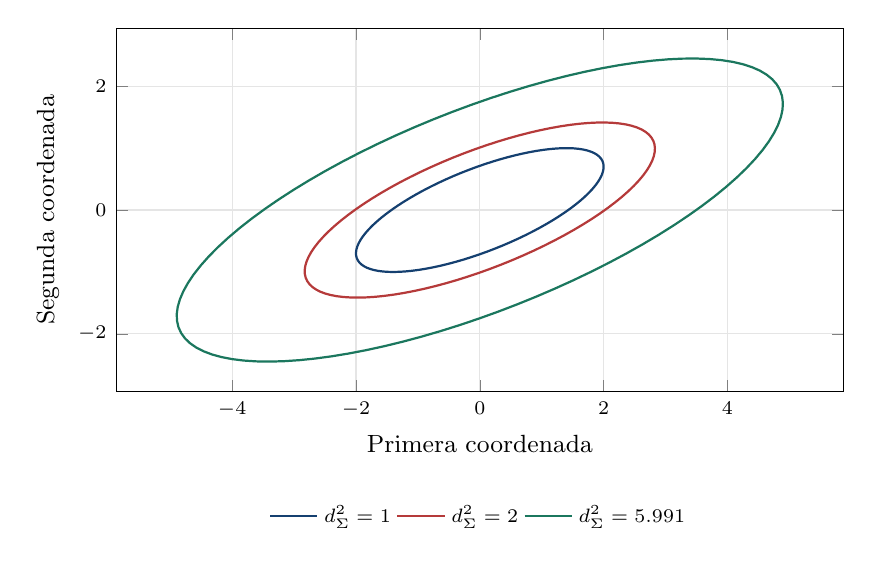
\begin{tikzpicture}
\begin{axis}[panelaxis,xlabel={Primera coordenada},ylabel={Segunda coordenada},axis equal image,width=11.5cm,height=6.2cm]
\addplot[azul,thick,no marks] coordinates {(0.245492746,-0.622820085) (0.119109864,-0.671186808) (-0.0077526305,-0.716850898) (-0.134583908,-0.759628483) (-0.260873264,-0.799347312) (-0.386112175,-0.835847451) (-0.509796349,-0.868981928) (-0.631427753,-0.898617321) (-0.75051662,-0.924634299) (-0.866583422,-0.946928101) (-0.979160798,-0.965408959) (-1.08779544,-0.980002455) (-1.19204991,-0.990649827) (-1.29150442,-0.997308201) (-1.3857585,-0.999950768) (-1.47443261,-0.998566886) (-1.55716971,-0.993162127) (-1.63363663,-0.983758255) (-1.70352548,-0.970393136) (-1.76655483,-0.953120586) (-1.82247088,-0.932010156) (-1.87104849,-0.90714685) (-1.91209205,-0.878630784) (-1.94543629,-0.846576781) (-1.97094694,-0.811113913) (-1.98852128,-0.772384975) (-1.99808855,-0.730545916) (-1.99961023,-0.685765206) (-1.99308018,-0.638223162) (-1.9785247,-0.588111218) (-1.95600239,-0.535631158) (-1.92560396,-0.4809943) (-1.8874518,-0.424420648) (-1.84169954,-0.366138004) (-1.7885314,-0.306381051) (-1.72816148,-0.24539041) (-1.66083286,-0.183411669) (-1.58681666,-0.120694393) (-1.5064109,-0.0574911239) (-1.41993936,0.00594364197) (-1.32775022,0.0693544749) (-1.2302147,0.132486042) (-1.12772555,0.195084134) (-1.02069544,0.256896692) (-0.909555345,0.317674817) (-0.794752796,0.377173777) (-0.676750058,0.435153992) (-0.556022286,0.491381996) (-0.433055608,0.545631378) (-0.308345169,0.597683694) (-0.182393132,0.64732935) (-0.0557066629,0.694368438) (0.0712041176,0.73861155) (0.197828184,0.779880534) (0.323655667,0.818009214) (0.448179902,0.85284406) (0.570899475,0.884244804) (0.691320237,0.912085006) (0.808957297,0.936252564) (0.923336971,0.956650163) (1.03399869,0.973195669) (1.14049687,0.98582246) (1.24240266,0.994479692) (1.33930574,0.999132505) (1.43081591,0.999762165) (1.51656469,0.996366135) (1.59620679,0.98895809) (1.66942154,0.97756786) (1.73591411,0.962241309) (1.79541677,0.943040152) (1.84768992,0.920041705) (1.89252308,0.893338575) (1.92973571,0.863038286) (1.95917798,0.829262846) (1.98073133,0.792148257) (1.99430897,0.751843967) (1.99985623,0.708512267) (1.99735078,0.662327638) (1.98680271,0.613476049) (1.96825448,0.562154209) (1.94178078,0.508568772) (1.90748822,0.452935508) (1.86551488,0.395478433) (1.81602976,0.336428906) (1.75923214,0.276024698) (1.69535071,0.214509036) (1.6246427,0.152129622) (1.54739282,0.0891376356) (1.46391215,0.0257867235) (1.37453681,-0.0376680227) (1.2796267,-0.100971093) (1.17956399,-0.163867588) (1.07475158,-0.226104247) (0.965611535,-0.287430463) (0.85258331,-0.347599299) (0.736122033,-0.406368474) (0.616696652,-0.463501347) (0.494788052,-0.518767864) (0.370887115,-0.571945486) (0.245492746,-0.622820085)};
\addlegendentry{$d_\Sigma^2=1$}
\addplot[rojo,thick,no marks] coordinates {(0.347179171,-0.880800612) (0.168446786,-0.949201487) (-0.0109638752,-1.01378026) (-0.190330388,-1.0742769) (-0.368930508,-1.13044781) (-0.546045075,-1.1820668) (-0.720960911,-1.22892603) (-0.892973692,-1.2708368) (-1.06139078,-1.30763037) (-1.22553403,-1.33915856) (-1.38474248,-1.36529444) (-1.53837506,-1.38593276) (-1.68581315,-1.40099042) (-1.82646307,-1.41040678) (-1.95975846,-1.41414394) (-2.0851626,-1.41218683) (-2.20217052,-1.40454335) (-2.31031108,-1.39124427) (-2.40914883,-1.37234313) (-2.49828579,-1.34791606) (-2.57736304,-1.3180614) (-2.64606215,-1.28289938) (-2.70410651,-1.24257157) (-2.75126238,-1.19724037) (-2.78733989,-1.1470883) (-2.81219377,-1.09231731) (-2.82572393,-1.03314794) (-2.8278759,-0.969818455) (-2.81864102,-0.902583851) (-2.79805646,-0.831714861) (-2.76620511,-0.757496848) (-2.72321524,-0.680228663) (-2.66925994,-0.600221437) (-2.60455646,-0.517797331) (-2.52936536,-0.433288238) (-2.4439894,-0.347034447) (-2.34877236,-0.25938327) (-2.24409764,-0.170687648) (-2.13038672,-0.0813047271) (-2.0080975,0.00840557908) (-1.87772237,0.098082039) (-1.73978632,0.187363557) (-1.59484476,0.275890628) (-1.44348133,0.363306785) (-1.28630551,0.449260034) (-1.12395018,0.533404271) (-0.95706911,0.615400678) (-0.786334258,0.694919083) (-0.612433115,0.771639294) (-0.43606592,0.845252386) (-0.257942841,0.915461946) (-0.0787811181,0.981985263) (0.100697829,1.04455447) (0.279771301,1.10291763) (0.457718233,1.15683973) (0.633822096,1.20610364) (0.80737378,1.25051099) (0.977674455,1.28988299) (1.14403838,1.32406107) (1.30579567,1.35290763) (1.46229498,1.37630651) (1.61290614,1.39416349) (1.7570227,1.40640667) (1.89406434,1.41298674) (2.02347926,1.41387721) (2.14474635,1.4090745) (2.25737729,1.39859794) (2.36091858,1.38248973) (2.45495328,1.36081471) (2.53910275,1.33366017) (2.61302814,1.30113546) (2.6764318,1.26337153) (2.72905841,1.22052045) (2.77069606,1.17275476) (2.8011771,1.12026681) (2.82037879,1.06326794) (2.82822381,1.00198766) (2.82468057,0.936672728) (2.80976334,0.867586149) (2.78353218,0.795006106) (2.74609272,0.719224855) (2.69759571,0.640547538) (2.63823644,0.559290963) (2.56825392,0.475782321) (2.48792995,0.390357871) (2.39758796,0.303361588) (2.29759174,0.215143775) (2.18834392,0.126059653) (2.07028441,0.0364679341) (1.9438886,-0.0532706285) (1.80966544,-0.142794689) (1.66815539,-0.231743766) (1.51992827,-0.319759692) (1.36558093,-0.406488059) (1.20573488,-0.491579642) (1.04103376,-0.574691808) (0.87214077,-0.655489892) (0.699735974,-0.73364855) (0.524513588,-0.808853064) (0.347179171,-0.880800612)};
\addlegendentry{$d_\Sigma^2=2$}
\addplot[verde,thick,no marks] coordinates {(0.600904091,-1.52450589) (0.291550793,-1.64289538) (-0.0189764767,-1.75466951) (-0.329427335,-1.85937821) (-0.638551705,-1.95659985) (-0.945104854,-2.04594295) (-1.2478524,-2.12704776) (-1.54557528,-2.1995877) (-1.83707468,-2.26327068) (-2.12117682,-2.31784026) (-2.39673774,-2.36307672) (-2.66264784,-2.3987979) (-2.91783639,-2.42485997) (-3.16127585,-2.44115799) (-3.39198597,-2.44762632) (-3.60903775,-2.44423893) (-3.81155722,-2.43100945) (-3.99872889,-2.40799115) (-4.16979909,-2.37527672) (-4.32407898,-2.33299789) (-4.46094732,-2.28132491) (-4.57985301,-2.22046583) (-4.68031725,-2.15066572) (-4.7619355,-2.07220563) (-4.82437912,-1.98540151) (-4.86739667,-1.89060288) (-4.89081493,-1.78819145) (-4.8945396,-1.67857961) (-4.87855569,-1.56220872) (-4.84292756,-1.43954737) (-4.78779866,-1.31108947) (-4.71339099,-1.17735227) (-4.62000416,-1.0388743) (-4.50801421,-0.896213139) (-4.37787207,-0.749943248) (-4.23010178,-0.6006536) (-4.06529837,-0.448945331) (-3.88412544,-0.295429319) (-3.68731251,-0.140723716) (-3.47565206,0.0145485308) (-3.2499964,0.169762196) (-3.01125414,0.324292289) (-2.76038663,0.477516571) (-2.49840402,0.628818062) (-2.22636121,0.777587526) (-1.94535364,0.923225918) (-1.65651281,1.06514681) (-1.36100179,1.20277872) (-1.06001049,1.33556748) (-0.75475091,1.46297837) (-0.446452212,1.58449836) (-0.136355807,1.69963814) (0.174289653,1.80793408) (0.484233311,1.90895011) (0.792227132,2.00227946) (1.09703093,2.08754635) (1.39741738,2.16440742) (1.69217692,2.23255318) (1.98012266,2.29170925) (2.26009514,2.3416374) (2.53096702,2.38213662) (2.79164759,2.4130438) (3.04108718,2.43423451) (3.27828139,2.44562342) (3.50227511,2.44716467) (3.7121664,2.43885205) (3.90711012,2.42071903) (4.08632128,2.39283863) (4.24907826,2.35532311) (4.39472571,2.30832354) (4.52267715,2.25202917) (4.63241736,2.18666667) (4.72350446,2.11249923) (4.79557168,2.0298255) (4.84832882,1.93897839) (4.88156346,1.84032369) (4.89514176,1.73425866) (4.88900905,1.62121038) (4.86319003,1.50163405) (4.81778866,1.37601118) (4.75298776,1.2448476) (4.66904825,1.10867145) (4.56630813,0.968031081) (4.4451811,0.823492787) (4.30615489,0.675638579) (4.14978932,0.525063813) (3.97671401,0.3723748) (3.78762588,0.218186365) (3.58328632,0.0631193707) (3.36451812,-0.0922017831) (3.1322022,-0.247151673) (2.88727401,-0.40110637) (2.63071978,-0.553445953) (2.36357258,-0.703557005) (2.0869081,-0.850835081) (1.80184037,-0.994687145) (1.50951728,-1.13453395) (1.21111589,-1.2698124) (0.907837759,-1.39997775) (0.600904091,-1.52450589)};
\addlegendentry{$d_\Sigma^2=5.991$}
\end{axis}
\end{tikzpicture}
\caption{Elipses de Mahalanobis para una normal con covarianza $\left(\begin{smallmatrix}4&1.4\\1.4&1\end{smallmatrix}\right)$. El contorno exterior corresponde aproximadamente a probabilidad conjunta $0.95$ en dos dimensiones.}\label{fig:panel-4}
\end{figure}
% FIN PANELFIG
\section{Chi-cuadrado, Student y Fisher desde normales}
Si $Z_1,\ldots,Z_\nu$ son normales estándar independientes, $U=\sum_jZ_j^2$ tiene distribución $\chi_\nu^2$. Su media es $\nu$ y su varianza $2\nu$, pues $\E Z^4=3$ se obtiene con otra integración por partes. Si $Z$ es estándar e independiente de $U$, entonces
\[
t_\nu=\frac Z{\sqrt{U/\nu}}
\]
define Student. Si $U_1\sim\chi_r^2$ y $U_2\sim\chi_\nu^2$ son independientes,
\[
F_{r,\nu}=\frac{U_1/r}{U_2/\nu}.
\]
La construcción explica las condiciones de independencia que se necesitan para contrastes exactos. Sustituir una varianza robusta en un cociente no produce automáticamente una distribución Student exacta con los grados de libertad de MCO.



% PANELFIG 22
\begin{figure}[htbp]\centering
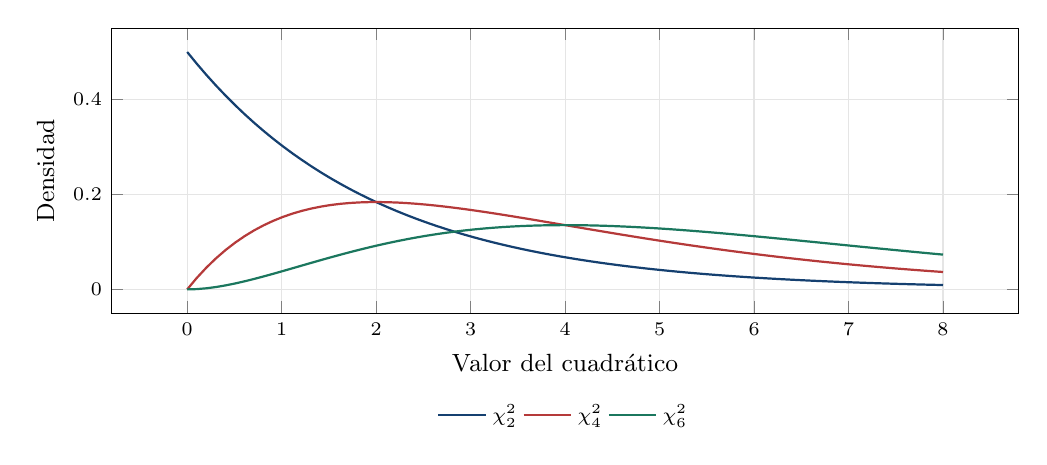
\begin{tikzpicture}
\begin{axis}[panelaxis,xlabel={Valor del cuadrático},ylabel={Densidad}]
\addplot[azul,thick,no marks] coordinates {(0,0.5) (0.101265823,0.475313786) (0.202531646,0.451846389) (0.303797468,0.429537636) (0.405063291,0.408330319) (0.506329114,0.38817006) (0.607594937,0.369005161) (0.708860759,0.35078648) (0.810126582,0.333467299) (0.911392405,0.317003209) (1.01265823,0.30135199) (1.11392405,0.286473511) (1.21518987,0.272329618) (1.3164557,0.258884043) (1.41772152,0.246102309) (1.51898734,0.23395164) (1.62025316,0.222400879) (1.72151899,0.211420408) (1.82278481,0.200982069) (1.92405063,0.191059096) (2.02531646,0.181626044) (2.12658228,0.172658725) (2.2278481,0.164134145) (2.32911392,0.156030443) (2.43037975,0.148326841) (2.53164557,0.141003585) (2.63291139,0.134041895) (2.73417722,0.127423921) (2.83544304,0.121132693) (2.93670886,0.115152078) (3.03797468,0.10946674) (3.13924051,0.104062101) (3.24050633,0.0989243022) (3.34177215,0.0940401692) (3.44303797,0.0893971776) (3.5443038,0.0849834218) (3.64556962,0.0807875838) (3.74683544,0.0767989046) (3.84810127,0.0730071561) (3.94936709,0.0694026155) (4.05063291,0.0659760398) (4.15189873,0.0627186425) (4.25316456,0.0596220707) (4.35443038,0.0566783843) (4.4556962,0.0538800348) (4.55696203,0.0512198466) (4.65822785,0.0486909984) (4.75949367,0.0462870055) (4.86075949,0.0440017036) (4.96202532,0.0418292326) (5.06329114,0.0397640218) (5.16455696,0.0378007755) (5.26582278,0.0359344594) (5.36708861,0.0341602878) (5.46835443,0.0324737114) (5.56962025,0.0308704054) (5.67088608,0.0293462585) (5.7721519,0.0278973625) (5.87341772,0.0265200019) (5.97468354,0.025210645) (6.07594937,0.0239659342) (6.17721519,0.0227826778) (6.27848101,0.0216578417) (6.37974684,0.0205885414) (6.48101266,0.0195720351) (6.58227848,0.0186057162) (6.6835443,0.0176871068) (6.78481013,0.0168138514) (6.88607595,0.0159837107) (6.98734177,0.0151945561) (7.08860759,0.014444364) (7.18987342,0.0137312106) (7.29113924,0.0130532674) (7.39240506,0.0124087959) (7.49367089,0.0117961435) (7.59493671,0.0112137392) (7.69620253,0.0106600897) (7.79746835,0.0101337752) (7.89873418,0.00963344608) (8,0.00915781944)};
\addlegendentry{$\chi^2_{2}$}
\addplot[rojo,thick,no marks] coordinates {(0,0) (0.101265823,0.0240665208) (0.202531646,0.0457565964) (0.303797468,0.0652462231) (0.405063291,0.0826998115) (0.506329114,0.0982709012) (0.607594937,0.112102834) (0.708860759,0.124329385) (0.810126582,0.135075362) (0.911392405,0.144457158) (1.01265823,0.152583286) (1.11392405,0.159554867) (1.21518987,0.165466097) (1.3164557,0.170404686) (1.41772152,0.17445227) (1.51898734,0.17768479) (1.62025316,0.180172864) (1.72151899,0.181982123) (1.82278481,0.183173531) (1.92405063,0.183803687) (2.02531646,0.183925108) (2.12658228,0.183586493) (2.2278481,0.182832971) (2.32911392,0.181706339) (2.43037975,0.180245275) (2.53164557,0.17848555) (2.63291139,0.176460217) (2.73417722,0.174199791) (2.83544304,0.171732425) (2.93670886,0.169084063) (3.03797468,0.166278592) (3.13924051,0.163337981) (3.24050633,0.160282414) (3.34177215,0.157130409) (3.44303797,0.153898939) (3.5443038,0.150603532) (3.64556962,0.147258381) (3.74683544,0.143876429) (3.84810127,0.140469465) (3.94936709,0.137048203) (4.05063291,0.133622359) (4.15189873,0.130200726) (4.25316456,0.126791239) (4.35443038,0.123401039) (4.4556962,0.120036533) (4.55696203,0.116703448) (4.65822785,0.113406882) (4.75949367,0.110151355) (4.86075949,0.106940849) (4.96202532,0.103778856) (5.06329114,0.10066841) (5.16455696,0.0976121291) (5.26582278,0.0946122474) (5.36708861,0.0916706458) (5.46835443,0.0887888819) (5.56962025,0.0859682176) (5.67088608,0.0832096444) (5.7721519,0.0805139069) (5.87341772,0.0778815246) (5.97468354,0.0753128129) (6.07594937,0.0728079015) (6.17721519,0.0703667518) (6.27848101,0.0679891739) (6.37974684,0.0656748411) (6.48101266,0.0634233038) (6.58227848,0.0612340028) (6.6835443,0.0591062811) (6.78481013,0.0570393946) (6.88607595,0.055032523) (6.98734177,0.0530847783) (7.08860759,0.051195214) (7.18987342,0.0493628331) (7.29113924,0.0475865951) (7.39240506,0.0458654228) (7.49367089,0.0441982085) (7.59493671,0.0425838199) (7.69620253,0.0410211046) (7.79746835,0.0395088956) (7.89873418,0.0380460149) (8,0.0366312778)};
\addlegendentry{$\chi^2_{4}$}
\addplot[verde,thick,no marks] coordinates {(0,0) (0.101265823,0.000609279007) (0.202531646,0.00231678969) (0.303797468,0.00495540935) (0.405063291,0.00837466446) (0.506329114,0.0124393546) (0.607594937,0.0170282785) (0.708860759,0.0220330556) (0.810126582,0.0273570353) (0.911392405,0.0329142893) (1.01265823,0.0386286801) (1.11392405,0.0444330008) (1.21518987,0.0502681813) (1.3164557,0.056082555) (1.41772152,0.0618311841) (1.51898734,0.0674752367) (1.62025316,0.0729814134) (1.72151899,0.0783214201) (1.82278481,0.0834714824) (1.92405063,0.0884119001) (2.02531646,0.0931266369) (2.12658228,0.0976029454) (2.2278481,0.101831022) (2.32911392,0.105803691) (2.43037975,0.109516117) (2.53164557,0.112965538) (2.63291139,0.116151029) (2.73417722,0.119073275) (2.83544304,0.121734377) (2.93670886,0.124137667) (3.03797468,0.126287538) (3.13924051,0.128189302) (3.24050633,0.129849044) (3.34177215,0.131273506) (3.44303797,0.132469972) (3.5443038,0.133446168) (3.64556962,0.13421017) (3.74683544,0.134770326) (3.84810127,0.135135181) (3.94936709,0.135313415) (4.05063291,0.135313781) (4.15189873,0.135145057) (4.25316456,0.134816001) (4.35443038,0.134335309) (4.4556962,0.133711581) (4.55696203,0.132953295) (4.65822785,0.132068774) (4.75949367,0.131066169) (4.86075949,0.129953437) (4.96202532,0.128738327) (5.06329114,0.127428367) (5.16455696,0.12603085) (5.26582278,0.124552832) (5.36708861,0.12300112) (5.46835443,0.121382269) (5.56962025,0.119702582) (5.67088608,0.117968104) (5.7721519,0.116184625) (5.87341772,0.114357682) (5.97468354,0.112492556) (6.07594937,0.110594281) (6.17721519,0.108667642) (6.27848101,0.106717184) (6.37974684,0.104747215) (6.48101266,0.102761809) (6.58227848,0.100764815) (6.6835443,0.098759862) (6.78481013,0.0967503656) (6.88607595,0.0947395332) (6.98734177,0.0927303722) (7.08860759,0.0907256957) (7.18987342,0.0887281304) (7.29113924,0.0867401227) (7.39240506,0.0847639459) (7.49367089,0.0828017071) (7.59493671,0.0808553542) (7.69620253,0.0789266823) (7.79746835,0.0770173408) (7.89873418,0.0751288395) (8,0.0732625556)};
\addlegendentry{$\chi^2_{6}$}
\end{axis}
\end{tikzpicture}
\caption{Distribuciones de sumas de cuadrados de normales independientes. El número de direcciones residuales identifica los grados de libertad de los contrastes clásicos.}\label{fig:panel-22}
\end{figure}
% FIN PANELFIG
\section{Formas cuadráticas: media y varianza}
Para $V=\mu+e$, $\E e=0$, $\Var(e)=\Sigma$, y una matriz simétrica $A$,
\[
\E(V\T AV)=\mu\T A\mu+\tr(A\Sigma).
\]
En efecto, el término lineal tiene media cero y
$\E(e\T Ae)=\sum_{j,k}A_{jk}\Sigma_{jk}=\tr(A\Sigma)$.
Si además $e$ es normal,
\[
\Var(V\T AV)=2\tr(A\Sigma A\Sigma)+4\mu\T A\Sigma A\mu.
\]
Una forma de deducir el primer término es diagonalizar
$\Sigma^{1/2}A\Sigma^{1/2}=Q\Lambda Q\T$: el cuadrático centrado es una suma $\sum_j\lambda_j(Z_j^2-1)$ de términos independientes de varianza $2\lambda_j^2$. El término lineal tiene varianza $4\mu\T A\Sigma A\mu$ y covarianza cero con el cuadrático por simetría de los terceros momentos normales.

\section{Diseño fijo, diseño aleatorio y dos esperanzas}
Si $\widehat\beta=A(X)y$, podemos estudiar su distribución condicionando en el diseño $X$. Bajo $\E(u\mid X)=0$,
$\E(\widehat\beta\mid X)=\beta$.
Para la varianza incondicional,
\[
\Var(\widehat\beta)
=\E[\Var(\widehat\beta\mid X)]
+\Var[\E(\widehat\beta\mid X)].
\]
Si la esperanza condicional es siempre $\beta$, el segundo término es cero; el primero sigue siendo una esperanza de matrices inversas. En general,
$\E[(X\T X)^{-1}]\ne[\E(X\T X)]^{-1}$.
Cuando una inversa aleatoria se acerca a singularidad, algunos momentos pueden no existir. Esta dificultad es especialmente relevante en IV débil.



% MODULO 03_mco_pooled.tex
\parte{III. Regresión clásica y pooled: derivar antes de estimar}
\section{La función objetivo de mínimos cuadrados ordinarios}
Sea $y_j=z_j\T b+u_j$, $j=1,\ldots,n$, con $z_j\in\R^p$. La matriz $Z$ apila $z_j\T$; puede incluir una constante. MCO minimiza
\[
S(b)=\sum_{j=1}^n\left(y_j-\sum_{k=1}^p z_{jk}b_k\right)^2
=(y-Zb)\T(y-Zb).
\]
La derivada respecto de $b_\ell$ es
\[
\frac{\partial S}{\partial b_\ell}
=-2\sum_{j=1}^n z_{j\ell}
\left(y_j-\sum_{k=1}^p z_{jk}b_k\right).
\]
Igualando las $p$ derivadas a cero:
$\sum_k(\sum_jz_{j\ell}z_{jk})\widehat b_k=\sum_jz_{j\ell}y_j$.
Son las ecuaciones normales $Z\T Z\widehat b=Z\T y$.
Si $\rank(Z)=p$,
\[
\widehat b=(Z\T Z)^{-1}Z\T y.
\]
El Hessiano es $2Z\T Z$; para todo $c\ne0$, $c\T Z\T Zc=\norm{Zc}^2>0$. Por ello la solución es un mínimo único. Si falla el rango, los valores ajustados aún pueden ser únicos, pero los coeficientes de una parametrización redundante no lo son.

\section{Una recta con intercepto, sin esconder ninguna sumatoria}
Con $z_j=(1,x_j)\T$ y $b=(c,\beta)\T$, las ecuaciones son
\[
n\widehat c+\left(\sum_jx_j\right)\widehat\beta=\sum_jy_j,
\quad
\left(\sum_jx_j\right)\widehat c+
\left(\sum_jx_j^2\right)\widehat\beta=\sum_jx_jy_j.
\]
La primera da $\widehat c=\bar y-\widehat\beta\bar x$. Sustituyendo en la segunda,
\[
\widehat\beta
=\frac{\sum_j(x_j-\bar x)(y_j-\bar y)}
{\sum_j(x_j-\bar x)^2}.
\]
No existe una pendiente única si todos los $x_j$ coinciden. El denominador mide la información geométrica en la columna residualizada respecto de la constante.

\begin{resuelto}{Pooled del panel de dos entidades}
Para $x=(1,2,3,2,3,4)\T$ y $y=(3,5,7,8,10,12)\T$,
\[
\sum_jx_j=15,\quad \sum_jy_j=45,\quad
\sum_jx_j^2=43,\quad \sum_jx_jy_j=128.
\]
El producto cruzado es $1(3)+2(5)+3(7)+2(8)+3(10)+4(12)=128$.
Entonces
\[
Z\T Z=\begin{pmatrix}6&15\\15&43\end{pmatrix},\quad
(Z\T Z)^{-1}=\frac1{33}\begin{pmatrix}43&-15\\-15&6\end{pmatrix},
\]
\[
\widehat b=\frac1{33}\begin{pmatrix}43(45)-15(128)\\-15(45)+6(128)\end{pmatrix}
=\frac1{33}\begin{pmatrix}15\\93\end{pmatrix}
=\begin{pmatrix}5/11\\31/11\end{pmatrix}.
\]
La pendiente pooled $31/11$ supera la pendiente individual $2$ porque las entidades con $x$ alto también tienen interceptos altos.
\end{resuelto}


\section{Proyectores, residuos y ortogonalidad}
Definimos
\[
P_Z=Z(Z\T Z)^{-1}Z\T,\qquad M_Z=I_n-P_Z.
\]
Se verifica $P_Z\T=P_Z$, $P_Z^2=P_Z$ y $M_Z^2=M_Z$.
Los valores ajustados son $\widehat y=P_Zy$; los residuos, $\widehat u=M_Zy$. Las ecuaciones normales equivalen a $Z\T\widehat u=0$.
Si hay una constante, $\sum_j\widehat u_j=0$. Esto es una identidad muestral; no prueba que $\E(u\mid Z)=0$.

El espacio de columnas $\mathcal C(Z)$ tiene dimensión $p$. Su complemento ortogonal tiene dimensión $n-p$. Por el teorema de Pitágoras,
\[
\norm y^2=\norm{P_Zy}^2+\norm{M_Zy}^2.
\]
Con intercepto, se aplica a $y-\bar y\ones$ para obtener la descomposición de suma de cuadrados total, explicada y residual. El coeficiente $R^2$ describe ajuste en esa geometría; no identifica un efecto causal.

\section{Esperanza, varianza y covarianza de todos los coeficientes}
Bajo $y=Zb+u$,
\[
\widehat b-b=A u,\qquad A=(Z\T Z)^{-1}Z\T.
\]
Condicionando en $Z$,
\[
\E(\widehat b\mid Z)=b+A\E(u\mid Z),\qquad
\Var(\widehat b\mid Z)=A\Omega A\T,
\]
donde $\Omega=\Var(u\mid Z)$. Con media condicional cero hay insesgadez. Con $\Omega=\sigma^2I_n$,
\[
V_b=\sigma^2(Z\T Z)^{-1}.
\]
El elemento diagonal $(k,k)$ es $\Var(\widehat b_k\mid Z)$; el elemento $(k,\ell)$ es $\Cov(\widehat b_k,\widehat b_\ell\mid Z)$. La diagonal sola no basta para estudiar sumas, diferencias o efectos marginales.

Con una recta:
\[
\begin{aligned}
\Var(\widehat\beta\mid Z)&=\frac{\sigma^2}{S_{xx}},\\
\Var(\widehat c\mid Z)&=\sigma^2\left(\frac1n+\frac{\bar x^2}{S_{xx}}\right),\\
\Cov(\widehat c,\widehat\beta\mid Z)&=-\frac{\sigma^2\bar x}{S_{xx}},
\end{aligned}
\qquad S_{xx}=\sum_j(x_j-\bar x)^2.
\]
Estas identidades se deducen invirtiendo la matriz $2\times2$ de productos cruzados. Si $\bar x=0$, intercepto y pendiente son incorrelacionados; bajo normalidad conjunta, independientes.

\section{Varianza residual y distribución exacta}
Como $M_ZZ=0$, $\widehat u=M_Zu$. Si $\Omega=\sigma^2I_n$,
\[
\E(\widehat u\T\widehat u\mid Z)
=\sigma^2\tr(M_Z)=\sigma^2(n-p).
\]
Así $s^2=\widehat u\T\widehat u/(n-p)$ es insesgado para $\sigma^2$. Bajo normalidad,
\[
\frac{(n-p)s^2}{\sigma^2}\sim\chi_{n-p}^2,
\quad
\widehat b\mid Z\sim N(b,\sigma^2(Z\T Z)^{-1}).
\]
Además $\widehat b$ y $\widehat u$ son independientes porque su covarianza contiene $Z\T M_Z=0$ y son conjuntamente normales. Por ello
\[
\frac{\widehat b_k-b_k}{s\sqrt{[(Z\T Z)^{-1}]_{kk}}}\sim t_{n-p}.
\]
Con heterocedasticidad o dependencia, ni el divisor $n-p$ ni esta Student exacta resuelven por sí solos la inferencia.

\section{Frisch--Waugh--Lovell: eliminar controles algebraicamente}
Particionemos $Z=[C,X]$, donde $C$ contiene controles y $X$ variables de interés. Minimizar $\norm{y-C\gamma-X\beta}^2$ respecto de $\gamma$, dado $\beta$, da
$\gamma(\beta)=(C\T C)^{-1}C\T(y-X\beta)$.
El residuo es $M_C(y-X\beta)$, por lo que
\[
\widehat\beta=(X\T M_CX)^{-1}X\T M_Cy.
\]
Se regresan las versiones de $X$ y $y$ residualizadas respecto de $C$. Residualizar únicamente $y$ deja $X$ con parte explicada por $C$ y cambia la respuesta. Este teorema permite deducir FE sin almacenar miles de dummies.

El bloque de covarianza de $\widehat\beta$ bajo errores esféricos es
$\sigma^2(X\T M_CX)^{-1}$. Puede obtenerse de la inversa particionada de $Z\T Z$ mediante el complemento de Schur. La misma matriz mide la variación de $X$ que queda después de controlar por $C$.

\section{Pooled con heterogeneidad individual omitida}
Supongamos $y=Zb+Da+\eps$, donde $Z$ incluye la constante y las variables observadas, pero no todas las dummies de entidad. Entonces
\[
\widehat b_{\rm P}-b=(Z\T Z)^{-1}Z\T Da+(Z\T Z)^{-1}Z\T\eps.
\]
Si $a$ es tratado como fijo, el primer término es una desviación determinista condicional al diseño. Si $a$ es aleatorio,
\[
\E(\widehat b_{\rm P}-b\mid Z)
=(Z\T Z)^{-1}Z\T D\E(a\mid Z)
\]
cuando $\E(\eps\mid Z)=0$. Pooled requiere restricciones sobre la heterogeneidad, o controles suficientes, para estimar la pendiente estructural. La ausencia de sesgo no se logra cambiando únicamente el estimador de varianza.

Para un regresor centrado, el límite de una pendiente pooled satisface
\[
\beta_{\rm P}^{*}
=\beta+\frac{\Cov(x_{it},a_i)}{\Var(x_{it})}
\]
si el muestreo y los momentos justifican ese límite y $\Cov(x_{it},\eps_{it})=0$. La ecuación describe un parámetro de proyección poblacional, no una expectativa exacta de un cociente muestral.

\section{Descomposición de la pendiente pooled}
Para un regresor e intercepto, escribimos $W_{xx}$ y $B_{xx}$ para las sumas de cuadrados dentro y entre ponderada por $T_i$, y $W_{xy},B_{xy}$ para los productos cruzados. Si ambas variaciones son positivas,
\[
\widehat\beta_{\rm P}
=\frac{W_{xy}+B_{xy}}{W_{xx}+B_{xx}}
=\omega\widehat\beta_{\rm W}+(1-\omega)\widehat\beta_{\rm B,w},
\quad
\omega=\frac{W_{xx}}{W_{xx}+B_{xx}}.
\]
Aquí $\widehat\beta_{\rm B,w}=B_{xy}/B_{xx}$. Es una identidad escalar. Con múltiples regresores no existe en general un único peso escalar que combine todos los coeficientes; aparecen matrices de pesos.

Una diferencia grande entre pendientes dentro y entre no prueba por sí sola qué mecanismo la causa. Puede reflejar confusión por $a_i$, errores de medición diferentes, heterogeneidad de pendientes o un modelo funcional incompleto.



% PANELFIG 2
\begin{figure}[htbp]\centering
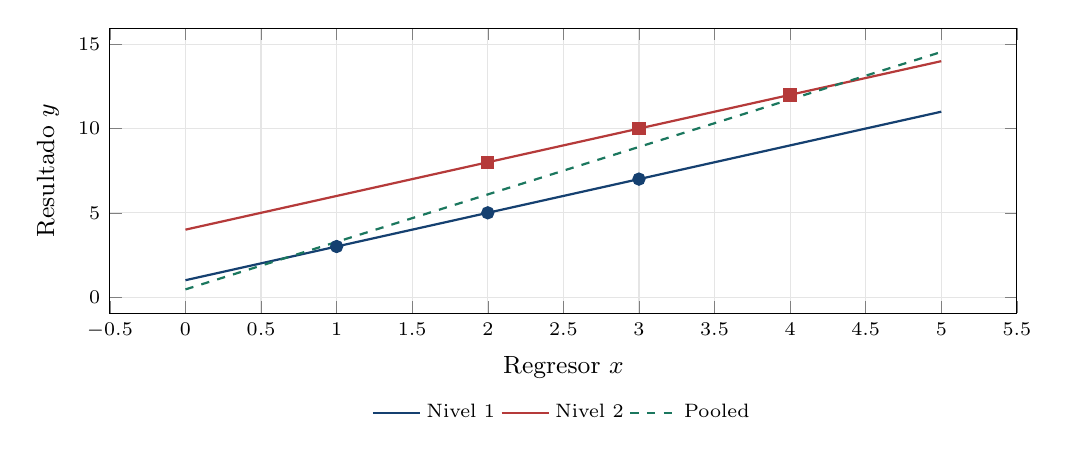
\begin{tikzpicture}
\begin{axis}[panelaxis,xlabel={Regresor $x$},ylabel={Resultado $y$}]
\addplot[azul,thick,no marks] coordinates {(0,1) (0.102040816,1.20408163) (0.204081633,1.40816327) (0.306122449,1.6122449) (0.408163265,1.81632653) (0.510204082,2.02040816) (0.612244898,2.2244898) (0.714285714,2.42857143) (0.816326531,2.63265306) (0.918367347,2.83673469) (1.02040816,3.04081633) (1.12244898,3.24489796) (1.2244898,3.44897959) (1.32653061,3.65306122) (1.42857143,3.85714286) (1.53061224,4.06122449) (1.63265306,4.26530612) (1.73469388,4.46938776) (1.83673469,4.67346939) (1.93877551,4.87755102) (2.04081633,5.08163265) (2.14285714,5.28571429) (2.24489796,5.48979592) (2.34693878,5.69387755) (2.44897959,5.89795918) (2.55102041,6.10204082) (2.65306122,6.30612245) (2.75510204,6.51020408) (2.85714286,6.71428571) (2.95918367,6.91836735) (3.06122449,7.12244898) (3.16326531,7.32653061) (3.26530612,7.53061224) (3.36734694,7.73469388) (3.46938776,7.93877551) (3.57142857,8.14285714) (3.67346939,8.34693878) (3.7755102,8.55102041) (3.87755102,8.75510204) (3.97959184,8.95918367) (4.08163265,9.16326531) (4.18367347,9.36734694) (4.28571429,9.57142857) (4.3877551,9.7755102) (4.48979592,9.97959184) (4.59183673,10.1836735) (4.69387755,10.3877551) (4.79591837,10.5918367) (4.89795918,10.7959184) (5,11)};
\addlegendentry{Nivel 1}
\addplot[rojo,thick,no marks] coordinates {(0,4) (0.102040816,4.20408163) (0.204081633,4.40816327) (0.306122449,4.6122449) (0.408163265,4.81632653) (0.510204082,5.02040816) (0.612244898,5.2244898) (0.714285714,5.42857143) (0.816326531,5.63265306) (0.918367347,5.83673469) (1.02040816,6.04081633) (1.12244898,6.24489796) (1.2244898,6.44897959) (1.32653061,6.65306122) (1.42857143,6.85714286) (1.53061224,7.06122449) (1.63265306,7.26530612) (1.73469388,7.46938776) (1.83673469,7.67346939) (1.93877551,7.87755102) (2.04081633,8.08163265) (2.14285714,8.28571429) (2.24489796,8.48979592) (2.34693878,8.69387755) (2.44897959,8.89795918) (2.55102041,9.10204082) (2.65306122,9.30612245) (2.75510204,9.51020408) (2.85714286,9.71428571) (2.95918367,9.91836735) (3.06122449,10.122449) (3.16326531,10.3265306) (3.26530612,10.5306122) (3.36734694,10.7346939) (3.46938776,10.9387755) (3.57142857,11.1428571) (3.67346939,11.3469388) (3.7755102,11.5510204) (3.87755102,11.755102) (3.97959184,11.9591837) (4.08163265,12.1632653) (4.18367347,12.3673469) (4.28571429,12.5714286) (4.3877551,12.7755102) (4.48979592,12.9795918) (4.59183673,13.1836735) (4.69387755,13.3877551) (4.79591837,13.5918367) (4.89795918,13.7959184) (5,14)};
\addlegendentry{Nivel 2}
\addplot[verde,thick,no marks,dashed] coordinates {(0,0.454545455) (0.102040816,0.742115028) (0.204081633,1.0296846) (0.306122449,1.31725417) (0.408163265,1.60482375) (0.510204082,1.89239332) (0.612244898,2.17996289) (0.714285714,2.46753247) (0.816326531,2.75510204) (0.918367347,3.04267161) (1.02040816,3.33024119) (1.12244898,3.61781076) (1.2244898,3.90538033) (1.32653061,4.19294991) (1.42857143,4.48051948) (1.53061224,4.76808905) (1.63265306,5.05565863) (1.73469388,5.3432282) (1.83673469,5.63079777) (1.93877551,5.91836735) (2.04081633,6.20593692) (2.14285714,6.49350649) (2.24489796,6.78107607) (2.34693878,7.06864564) (2.44897959,7.35621521) (2.55102041,7.64378479) (2.65306122,7.93135436) (2.75510204,8.21892393) (2.85714286,8.50649351) (2.95918367,8.79406308) (3.06122449,9.08163265) (3.16326531,9.36920223) (3.26530612,9.6567718) (3.36734694,9.94434137) (3.46938776,10.2319109) (3.57142857,10.5194805) (3.67346939,10.8070501) (3.7755102,11.0946197) (3.87755102,11.3821892) (3.97959184,11.6697588) (4.08163265,11.9573284) (4.18367347,12.244898) (4.28571429,12.5324675) (4.3877551,12.8200371) (4.48979592,13.1076067) (4.59183673,13.3951763) (4.69387755,13.6827458) (4.79591837,13.9703154) (4.89795918,14.257885) (5,14.5454545)};
\addlegendentry{Pooled}
\addplot[orange,thick,only marks,mark=*,azul] coordinates {(1,3) (2,5) (3,7)};
\addplot[azul,thick,only marks,mark=square*,rojo] coordinates {(2,8) (3,10) (4,12)};
\end{axis}
\end{tikzpicture}
\caption{El panel inicial tiene pendiente dentro igual a $2$, pero su pendiente pooled es $31/11$. Las rectas y los seis puntos usan exactamente los datos del ejemplo.}\label{fig:panel-2}
\end{figure}
% FIN PANELFIG
\section{Gauss--Markov demostrado con una perturbación}
Sea $C y$ cualquier estimador lineal insesgado de $b$, de modo que $CZ=I_p$. Escribamos $C=A+H$ con $A=(Z\T Z)^{-1}Z\T$. Entonces $HZ=0$.
Con $\Var(u\mid Z)=\sigma^2I_n$,
\[
\Var(Cy\mid Z)=\sigma^2AA\T+\sigma^2HH\T
+\sigma^2(AH\T+HA\T).
\]
Los términos cruzados desaparecen porque $AH\T=(Z\T Z)^{-1}Z\T H\T=0$.
Por tanto,
$\Var(Cy\mid Z)-\Var(\widehat b\mid Z)=\sigma^2HH\T$ es semidefinida positiva. MCO tiene mínima covarianza en esa clase bajo errores esféricos. GLS tiene la propiedad análoga tras blanquear; una regresión endógena queda fuera de la clase insesgada.

\section{Restricciones lineales, efectos marginales y predicción}
Para $L\in\R^{r\times p}$, $\widehat q=L\widehat b$ tiene
$\E(\widehat q\mid Z)=Lb$ y $\Var(\widehat q\mid Z)=LV_bL\T$.
En un cuadrático $m(x)=b_0+b_1x+b_2x^2$,
\[
m'(x)=b_1+2xb_2,\quad
\Var[\widehat m'(x)]=V_{11}+4x^2V_{22}+4xV_{12},
\]
donde esos índices se refieren a las dos pendientes. Ignorar su covarianza puede aumentar o disminuir la incertidumbre reportada.

La media predicha en una fila nueva $z_0$ es $z_0\T\widehat b$ y tiene varianza $z_0\T V_bz_0$. Si una observación futura incorpora un error independiente de varianza $\sigma_0^2$, el error de predicción tiene varianza $\sigma_0^2+z_0\T V_bz_0$. En panel, la independencia con el futuro puede fallar y un efecto individual adicional puede ser necesario.



% MODULO 04_fe_fd.tex
\parte{IV. Efectos fijos: quitar lo permanente sin perder la ecuación}
\section{El modelo de interceptos individuales}
El modelo estático de efectos fijos es
\[
y_{it}=a_i+x_{it}\T\beta+\eps_{it}.
\]
$a_i$ puede estar correlacionado con toda la trayectoria de $x_i$. Para identificar la pendiente imponemos restricciones sobre $\eps_{it}$, no sobre esa correlación. Una condición suficiente es
$\E(\eps_i\mid X_i,a_i)=0$, donde $X_i$ apila todos los regresores observados de $i$. La variación temporal necesaria está en $x_{it}-\bar x_i$.

Restando la media de la ecuación de cada entidad,
\[
y_{it}-\bar y_i=(x_{it}-\bar x_i)\T\beta+(\eps_{it}-\bar\eps_i).
\]
El intercepto desaparece porque $a_i-a_i=0$. Una variable $z_i$ constante en el tiempo también desaparece, incluso si su efecto verdadero no es cero. FE no estima el coeficiente separado de esa variable: es colineal con los interceptos.

\section{El aniquilador within y su rango}
Para cada entidad,
\[
J_i=\frac{\ones_{T_i}\ones_{T_i}\T}{T_i},\qquad
M_i=I_{T_i}-J_i.
\]
$J_i$ reemplaza cada vector por su media repetida y $M_i$ resta esa media. Con tres períodos,
\[
J_3=\frac13\begin{pmatrix}1&1&1\\1&1&1\\1&1&1\end{pmatrix},
\quad
M_3=\frac13\begin{pmatrix}2&-1&-1\\-1&2&-1\\-1&-1&2\end{pmatrix}.
\]
$J_i^2=J_i$ porque $\ones\T\ones=T_i$; por ello $M_i^2=M_i$. También $M_i\ones=0$. La dirección de la media tiene autovalor cero en $M_i$ y las $T_i-1$ direcciones de suma cero tienen autovalor uno. En consecuencia $\rank(M_i)=T_i-1$.

Apilando,
\[
M_D=I_n-D(D\T D)^{-1}D\T
=\diag(M_1,\ldots,M_G),\qquad \rank(M_D)=n-G.
\]
Esta fórmula sirve para panel desbalanceado porque $D\T D=\diag(T_1,\ldots,T_G)$, suponiendo al menos una fila por entidad. Una entidad con una sola fila tiene bloque $M_i=0$ y no aporta variación within a las pendientes.

\section{Estimador within y equivalencia con LSDV}
Aplicando Frisch--Waugh--Lovell al diseño $[D,X]$,
\[
\widehat\beta_{\rm FE}
=(X\T M_DX)^{-1}X\T M_Dy.
\]
Si $\widetilde X=M_DX$ y $\widetilde y=M_Dy$, la identidad $M_D^2=M_D$ permite escribir
\[
\widehat\beta_{\rm FE}
=(\widetilde X\T\widetilde X)^{-1}\widetilde X\T\widetilde y.
\]
Es exactamente la pendiente del modelo con dummies individuales, llamado LSDV. La matriz invertida es $K\times K$, aunque existan millones de filas y muchas entidades.

En componentes,
\[
\sum_{\ell=1}^K
\left[
\sum_{i=1}^G\sum_{t\in\mathcal T_i}
(x_{it,k}-\bar x_{i,k})(x_{it,\ell}-\bar x_{i,\ell})
\right]\widehat\beta_\ell
=\sum_i\sum_t(x_{it,k}-\bar x_{i,k})(y_{it}-\bar y_i).
\]
El rango exige que ninguna combinación lineal de las columnas de $X$ sea constante dentro de todas las entidades. No basta que la matriz original $X$ tenga rango completo.

\begin{resuelto}{Within con seis filas y todas las desviaciones}
Para el panel del inicio,
\[
\bar x_1=2,\quad\bar y_1=5,\qquad
\bar x_2=3,\quad\bar y_2=10.
\]
Las columnas transformadas son
\[
\widetilde x=\begin{pmatrix}-1\\0\\1\\-1\\0\\1\end{pmatrix},
\qquad
\widetilde y=\begin{pmatrix}-2\\0\\2\\-2\\0\\2\end{pmatrix}.
\]
Por tanto,
\[
\widetilde x\T\widetilde x
=(-1)^2+0^2+1^2+(-1)^2+0^2+1^2=4,
\]
\[
\widetilde x\T\widetilde y
=(-1)(-2)+0(0)+1(2)+(-1)(-2)+0(0)+1(2)=8.
\]
La pendiente es $8/4=2$. Los interceptos recuperados son
$\widehat a_1=5-2(2)=1$ y $\widehat a_2=10-2(3)=4$.
Todos los residuos son cero porque estos datos sintéticos se construyeron exactamente con esas rectas. No permiten estimar una varianza de error positiva a partir de sus residuos.
\end{resuelto}

\section{Esperanza de FE y el papel de la condición estricta}
Definimos $Q=X\T M_DX$ y $A_{\rm FE}=Q^{-1}X\T M_D$. Entonces
\[
\widehat\beta_{\rm FE}-\beta=A_{\rm FE}\eps.
\]
Como $A_{\rm FE}D=0$, cualquier magnitud de $a_i$ desaparece. Si
$\E(\eps\mid X,a)=0$,
\[
\E(\widehat\beta_{\rm FE}\mid X,a)=\beta.
\]
La media condicional de cada $\eps_{it}$ respecto de todos los regresores observados es suficiente para pasar la esperanza a través de $A_{\rm FE}$.

La ortogonalidad transformada necesaria para consistencia puede ser más débil que la media condicional nula completa, pero debe verificarse explícitamente:
$\E(X_i\T M_i\eps_i)=0$.
No es válido sustituirla sin prueba por $\E(x_{it}\eps_{it})=0$.

\section{Covarianza de FE: la matriz general y el caso esférico}
Con $\Omega=\Var(\eps\mid X,a)$,
\[
V_{\rm FE}=Q^{-1}X\T M_D\Omega M_DXQ^{-1}.
\]
La simetría de $Q$ se ha usado para escribir $Q^{-1}$ a ambos lados.
Si $\Omega=\sigma_\eps^2I_n$, $M_D^2=M_D$ produce
\[
V_{\rm FE}=\sigma_\eps^2Q^{-1}.
\]
Para cada par de pendientes,
\[
\Cov(\widehat\beta_k,\widehat\beta_\ell\mid X,a)
=\sigma_\eps^2[Q^{-1}]_{k\ell}.
\]
Con dependencia por entidad y entidades independientes,
\[
V_{\rm FE}
=Q^{-1}\left(\sum_{i=1}^G X_i\T M_i\Omega_iM_iX_i\right)Q^{-1}.
\]
Los errores transformados no son independientes aunque los originales lo fueran. Para $t\ne s$,
\[
\Cov(\eps_{it}-\bar\eps_i,\eps_{is}-\bar\eps_i)
=-\frac{\sigma_\eps^2}{T_i};
\quad
\Var(\eps_{it}-\bar\eps_i)=\sigma_\eps^2\left(1-\frac1{T_i}\right).
\]
La matriz $\sigma_\eps^2M_i$ es singular. No se debe tratar como $\sigma_\eps^2I_{T_i}$.

\section{Interceptos recuperados: medias, varianzas y covarianzas}
El vector de interceptos LSDV es
\[
\widehat a=(D\T D)^{-1}D\T(y-X\widehat\beta).
\]
Sea $H=(D\T D)^{-1}D\T$ y $B=HX$, cuyas filas son $\bar x_i\T$.
Entonces
\[
\widehat a-a=H\eps-B(\widehat\beta-\beta).
\]
Bajo errores esféricos, $\Cov(H\eps,\widehat\beta-\beta)=0$ porque
$HM_D=0$. Por ello
\[
\begin{aligned}
\E(\widehat a\mid X,a)&=a,\\
\Var(\widehat a\mid X,a)&=\sigma_\eps^2(D\T D)^{-1}+BV_{\rm FE}B\T,\\
\Cov(\widehat a,\widehat\beta\mid X,a)&=-BV_{\rm FE}.
\end{aligned}
\]
En particular,
\[
\begin{aligned}
\Var(\widehat a_i)&=\sigma_\eps^2/T_i+\bar x_i\T V_{\rm FE}\bar x_i,\\
\Cov(\widehat a_i,\widehat a_j)&=\bar x_i\T V_{\rm FE}\bar x_j\quad(i\ne j),\\
\Cov(\widehat a_i,\widehat\beta_k)&=-[\bar x_i\T V_{\rm FE}]_k.
\end{aligned}
\]
Las medias de errores de entidades distintas son independientes, pero los interceptos estimados comparten la misma pendiente estimada. Esa pendiente crea covarianzas entre ellos.

Con $\Omega$ general, sea $C=H\Omega A_{\rm FE}\T$.
Entonces
\[
\Var(\widehat a)=H\Omega H\T+BV_{\rm FE}B\T-CB\T-BC\T,
\quad
\Cov(\widehat a,\widehat\beta)=C-BV_{\rm FE}.
\]
Las dos fórmulas muestran qué términos se estaban anulando bajo esfericidad.

\section{Grados de libertad y varianza residual en FE}
Si $\rank([D,X])=G+K$, el proyector residual del modelo completo es
\[
M_{[D,X]}=M_D-M_DXQ^{-1}X\T M_D.
\]
Es simétrico e idempotente y tiene rango $n-G-K$. El residuo FE coincide con el residuo LSDV:
$\widehat\eps=M_{[D,X]}y$.
Por tanto, con errores esféricos,
\[
s_\eps^2=\frac{\sum_i\sum_t\widehat\eps_{it}^2}{n-G-K}
\]
es insesgado. Usar $n-K$ olvida los $G$ interceptos absorbidos.

Si $\eps\mid X,a$ es normal,
\[
\widehat\beta\sim N(\beta,\sigma_\eps^2Q^{-1}),\qquad
\frac{(n-G-K)s_\eps^2}{\sigma_\eps^2}\sim\chi_{n-G-K}^2.
\]
El residuo y los coeficientes del modelo completo son independientes. Se obtienen Student y Fisher exactas con los grados de libertad correctos. Bajo heterocedasticidad o correlación temporal, este cálculo exacto deja de ser aplicable y se requiere una covarianza adecuada.

\section{Por qué los interceptos no se vuelven precisos con muchos individuos}
Si $T_i=T$ es fijo y $G\to\infty$, la pendiente común puede ser consistente porque combina muchas entidades. Pero, incluso si $\beta$ se conociera,
$\widehat a_i=a_i+\bar\eps_i$ tendría varianza $\sigma_\eps^2/T$.
Esa varianza no tiende a cero al aumentar $G$. Es una manifestación del problema de parámetros incidentales. En el modelo lineal estático, la transformación elimina esos parámetros sin sesgar necesariamente la pendiente; en modelos no lineales la eliminación requiere otras herramientas.

\section{Primera diferencia: eliminar con otro operador}
Para una entidad con tres períodos,
\[
F_3=\begin{pmatrix}-1&1&0\\0&-1&1\end{pmatrix},
\qquad
F_3y_i=\begin{pmatrix}y_{i2}-y_{i1}\\y_{i3}-y_{i2}\end{pmatrix}.
\]
Como $F_3\ones_3=0$, se elimina $a_i$. La ecuación es
$\Delta y_{it}=\Delta x_{it}\T\beta+\Delta\eps_{it}$.
MCO en diferencias estima
\[
\widehat\beta_{\rm FD}
=\left(\sum_iX_i\T F_i\T F_iX_i\right)^{-1}
\sum_iX_i\T F_i\T F_iy_i.
\]
Con $T=2$, $F_2\T F_2=2M_2$, y el factor común se cancela: FE y FD tienen las mismas pendientes. Con $T>2$ las matrices no son proporcionales en general y las pendientes pueden diferir.

\section{Dependencia inducida por las diferencias}
Si los $\eps_{it}$ son independientes con varianza $\sigma_\eps^2$,
\[
\Var(\Delta\eps_{it})=2\sigma_\eps^2,\qquad
\Cov(\Delta\eps_{it},\Delta\eps_{i,t-1})=-\sigma_\eps^2.
\]
Para tres períodos,
\[
\Var(F_3\eps_i)=\sigma_\eps^2
\begin{pmatrix}2&-1\\-1&2\end{pmatrix}.
\]
FD-MCO ignora esa estructura si usa una varianza esférica. GLS en diferencias con la matriz $F_iF_i\T$ sí usa el peso correcto. Cuando $F_i$ tiene rango $T_i-1$,
\[
F_i\T(F_iF_i\T)^{-1}F_i=M_i.
\]
Ambos lados son el proyector ortogonal sobre el subespacio de suma cero. Así FD-GLS coincide con FE bajo errores originales esféricos.

Si el error original es un paseo aleatorio $\eps_{it}=\eps_{i,t-1}+\eta_{it}$ con incrementos independientes, las diferencias tienen errores $\eta_{it}$ esféricos. En ese caso FD puede ser más eficiente que FE-MCO. La comparación de eficiencia depende del proceso del error.



% PANELFIG 10
\begin{figure}[htbp]\centering
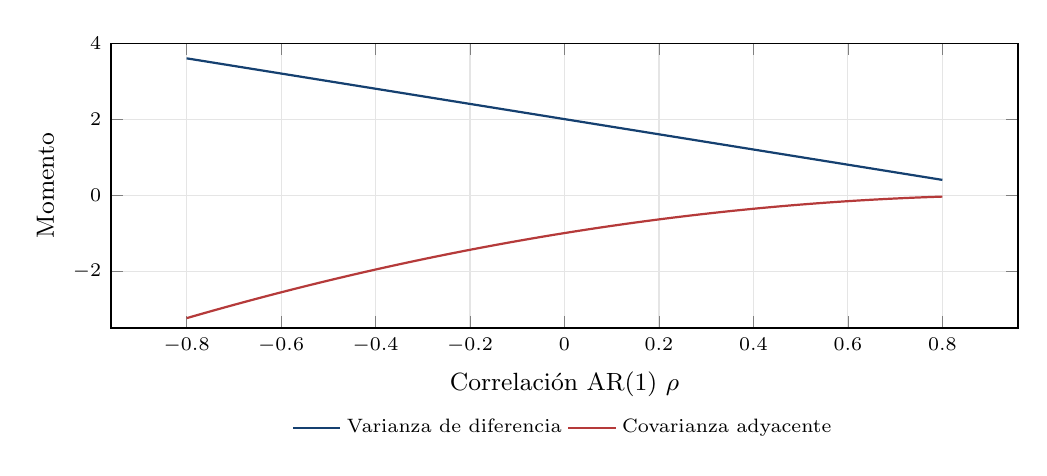
\begin{tikzpicture}
\begin{axis}[panelaxis,xlabel={Correlación AR(1) $\rho$},ylabel={Momento},ymin=-3.5,ymax=4]
\addplot[azul,thick,no marks] coordinates {(-0.8,3.6) (-0.779746835,3.55949367) (-0.759493671,3.51898734) (-0.739240506,3.47848101) (-0.718987342,3.43797468) (-0.698734177,3.39746835) (-0.678481013,3.35696203) (-0.658227848,3.3164557) (-0.637974684,3.27594937) (-0.617721519,3.23544304) (-0.597468354,3.19493671) (-0.57721519,3.15443038) (-0.556962025,3.11392405) (-0.536708861,3.07341772) (-0.516455696,3.03291139) (-0.496202532,2.99240506) (-0.475949367,2.95189873) (-0.455696203,2.91139241) (-0.435443038,2.87088608) (-0.415189873,2.83037975) (-0.394936709,2.78987342) (-0.374683544,2.74936709) (-0.35443038,2.70886076) (-0.334177215,2.66835443) (-0.313924051,2.6278481) (-0.293670886,2.58734177) (-0.273417722,2.54683544) (-0.253164557,2.50632911) (-0.232911392,2.46582278) (-0.212658228,2.42531646) (-0.192405063,2.38481013) (-0.172151899,2.3443038) (-0.151898734,2.30379747) (-0.13164557,2.26329114) (-0.111392405,2.22278481) (-0.0911392405,2.18227848) (-0.0708860759,2.14177215) (-0.0506329114,2.10126582) (-0.0303797468,2.06075949) (-0.0101265823,2.02025316) (0.0101265823,1.97974684) (0.0303797468,1.93924051) (0.0506329114,1.89873418) (0.0708860759,1.85822785) (0.0911392405,1.81772152) (0.111392405,1.77721519) (0.13164557,1.73670886) (0.151898734,1.69620253) (0.172151899,1.6556962) (0.192405063,1.61518987) (0.212658228,1.57468354) (0.232911392,1.53417722) (0.253164557,1.49367089) (0.273417722,1.45316456) (0.293670886,1.41265823) (0.313924051,1.3721519) (0.334177215,1.33164557) (0.35443038,1.29113924) (0.374683544,1.25063291) (0.394936709,1.21012658) (0.415189873,1.16962025) (0.435443038,1.12911392) (0.455696203,1.08860759) (0.475949367,1.04810127) (0.496202532,1.00759494) (0.516455696,0.967088608) (0.536708861,0.926582278) (0.556962025,0.886075949) (0.57721519,0.84556962) (0.597468354,0.805063291) (0.617721519,0.764556962) (0.637974684,0.724050633) (0.658227848,0.683544304) (0.678481013,0.643037975) (0.698734177,0.602531646) (0.718987342,0.562025316) (0.739240506,0.521518987) (0.759493671,0.481012658) (0.779746835,0.440506329) (0.8,0.4)};
\addlegendentry{Varianza de diferencia}
\addplot[rojo,thick,no marks] coordinates {(-0.8,-3.24) (-0.779746835,-3.1674988) (-0.759493671,-3.09581798) (-0.739240506,-3.02495754) (-0.718987342,-2.95491748) (-0.698734177,-2.8856978) (-0.678481013,-2.81729851) (-0.658227848,-2.7497196) (-0.637974684,-2.68296106) (-0.617721519,-2.61702291) (-0.597468354,-2.55190514) (-0.57721519,-2.48760776) (-0.556962025,-2.42413075) (-0.536708861,-2.36147412) (-0.516455696,-2.29963788) (-0.496202532,-2.23862202) (-0.475949367,-2.17842653) (-0.455696203,-2.11905143) (-0.435443038,-2.06049672) (-0.415189873,-2.00276238) (-0.394936709,-1.94584842) (-0.374683544,-1.88975485) (-0.35443038,-1.83448165) (-0.334177215,-1.78002884) (-0.313924051,-1.72639641) (-0.293670886,-1.67358436) (-0.273417722,-1.62159269) (-0.253164557,-1.57042141) (-0.232911392,-1.5200705) (-0.212658228,-1.47053998) (-0.192405063,-1.42182983) (-0.172151899,-1.37394007) (-0.151898734,-1.32687069) (-0.13164557,-1.2806217) (-0.111392405,-1.23519308) (-0.0911392405,-1.19058484) (-0.0708860759,-1.14679699) (-0.0506329114,-1.10382951) (-0.0303797468,-1.06168242) (-0.0101265823,-1.02035571) (0.0101265823,-0.979849383) (0.0303797468,-0.940163435) (0.0506329114,-0.901297869) (0.0708860759,-0.863252684) (0.0911392405,-0.82602788) (0.111392405,-0.789623458) (0.13164557,-0.754039417) (0.151898734,-0.719275757) (0.172151899,-0.685332479) (0.192405063,-0.652209582) (0.212658228,-0.619907066) (0.232911392,-0.588424932) (0.253164557,-0.557763179) (0.273417722,-0.527921807) (0.293670886,-0.498900817) (0.313924051,-0.470700208) (0.334177215,-0.443319981) (0.35443038,-0.416760135) (0.374683544,-0.39102067) (0.394936709,-0.366101586) (0.415189873,-0.342002884) (0.435443038,-0.318724563) (0.455696203,-0.296266624) (0.475949367,-0.274629066) (0.496202532,-0.253811889) (0.516455696,-0.233815094) (0.536708861,-0.21463868) (0.556962025,-0.196282647) (0.57721519,-0.178746996) (0.597468354,-0.162031726) (0.617721519,-0.146136837) (0.637974684,-0.13106233) (0.658227848,-0.116808204) (0.678481013,-0.103374459) (0.698734177,-0.090761096) (0.718987342,-0.0789681141) (0.739240506,-0.0679955135) (0.759493671,-0.0578432943) (0.779746835,-0.0485114565) (0.8,-0.04)};
\addlegendentry{Covarianza adyacente}
\end{axis}
\end{tikzpicture}
\caption{Si el error original es AR(1) con varianza marginal uno, las diferencias tienen varianza $2(1-\rho)$ y covarianza adyacente $-(1-\rho)^2$. Diferenciar induce dependencia incluso cuando $\rho=0$.}\label{fig:panel-10}
\end{figure}
% FIN PANELFIG
\section{Diferencias ortogonales hacia adelante}
Para panel balanceado, definimos
\[
h_{it}=\sqrt{\frac{T-t}{T-t+1}}
\left(v_{it}-\frac1{T-t}\sum_{s=t+1}^T v_{is}\right),
\quad t=1,\ldots,T-1.
\]
Los coeficientes de cada fila suman cero, eliminando un intercepto. Las filas tienen norma uno y son mutuamente ortogonales. Para $T=3$,
\[
H_3=\begin{pmatrix}
\sqrt{2/3}&-\sqrt{1/6}&-\sqrt{1/6}\\
0&1/\sqrt2&-1/\sqrt2
\end{pmatrix},
\quad H_3H_3\T=I_2,\quad H_3\T H_3=M_3.
\]
Con errores esféricos, $\Var(H_3\eps_i)=\sigma_\eps^2I_2$.
Esta transformación muestra que la singularidad within no implica falta de información adicional: las $T-1$ coordenadas ortogonales representan toda la variación temporal identificable.

\section{Una variable casi constante y el costo de identificarla}
Para un regresor $x_{it}=z_i+\delta w_{it}$, $M_ix_i=\delta M_iw_i$.
La información within es
$Q=\delta^2\sum_iw_i\T M_iw_i$.
Así
$\Var(\widehat\beta_{\rm FE})=\sigma_\eps^2/[\delta^2\sum_iw_i\T M_iw_i]$.
Cuando $\delta\to0$, la varianza crece como $\delta^{-2}$. La eliminación de confusión permanente tiene un costo cuando casi toda la variación es entre entidades.

El error de medición puede agravarlo. Si observamos $x_{it}^{\rm obs}=x_{it}+\eta_{it}$ y la señal verdadera varía poco en el tiempo, las desviaciones de $\eta$ pueden dominar la señal within. FE elimina una fuente de sesgo y puede aumentar la atenuación por otra.



% PANELFIG 6
\begin{figure}[htbp]\centering
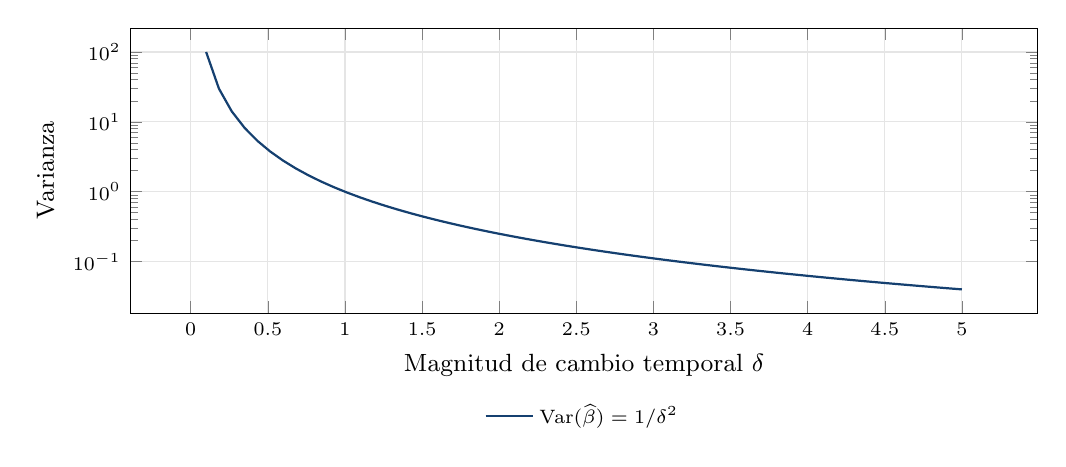
\begin{tikzpicture}
\begin{axis}[panelaxis,xlabel={Magnitud de cambio temporal $\delta$},ylabel={Varianza},ymode=log,ytick={0.1,1,10,100}]
\addplot[azul,thick,no marks] coordinates {(0.1,100) (0.183050847,29.8439643) (0.266101695,14.1222768) (0.349152542,8.2029409) (0.43220339,5.35332564) (0.515254237,3.76666378) (0.598305085,2.79353819) (0.681355932,2.15403084) (0.76440678,1.71139768) (0.847457627,1.3924) (0.930508475,1.15493976) (1.01355932,0.973423116) (1.09661017,0.831563583) (1.17966102,0.718597239) (1.26271186,0.627178956) (1.34576271,0.552157554) (1.42881356,0.489833941) (1.51186441,0.43749623) (1.59491525,0.393119672) (1.6779661,0.35516784) (1.76101695,0.322457831) (1.8440678,0.29406696) (1.92711864,0.269266977) (2.01016949,0.247476887) (2.09322034,0.228228622) (2.17627119,0.211141681) (2.25932203,0.19590419) (2.34237288,0.182258561) (2.42542373,0.169990541) (2.50847458,0.158920745) (2.59152542,0.148898064) (2.67457627,0.139794481) (2.75762712,0.131500958) (2.84067797,0.123924163) (2.92372881,0.116983827) (3.00677966,0.110610611) (3.08983051,0.104744369) (3.17288136,0.0993327215) (3.2559322,0.0943298825) (3.33898305,0.0896956891) (3.4220339,0.0853947921) (3.50508475,0.0813959796) (3.58813559,0.07767161) (3.67118644,0.074197132) (3.75423729,0.07095068) (3.83728814,0.0679127283) (3.92033898,0.0650657976) (4.00338983,0.0623942023) (4.08644068,0.0598838347) (4.16949153,0.0575219777) (4.25254237,0.0552971439) (4.33559322,0.0531989356) (4.41864407,0.0512179228) (4.50169492,0.0493455373) (4.58474576,0.0475739799) (4.66779661,0.0458961389) (4.75084746,0.0443055189) (4.83389831,0.0427961776) (4.91694915,0.0413626701) (5,0.04)};
\addlegendentry{$\Var(\widehat\beta)=1/\delta^2$}
\end{axis}
\end{tikzpicture}
\caption{Con información base unitaria, la varianza FE crece como $\delta^{-2}$ cuando la variable se vuelve casi invariante en el tiempo.}\label{fig:panel-6}
\end{figure}
% FIN PANELFIG
\section{Between: estimar con medias y entender la limitación}
Promediando:
\[
\bar y_i=a_i+\bar x_i\T\beta+\bar\eps_i.
\]
Una regresión de medias utiliza $G$ filas. Si $a_i$ está correlacionado con $\bar x_i$, between no identifica la pendiente estructural. Con $a_i$ aleatorio independiente de regresores,
\[
\Var(a_i+\bar\eps_i)=\sigma_a^2+\sigma_\eps^2/T_i.
\]
En panel desbalanceado, una regresión de medias sin pesos no es GLS eficiente bajo ese modelo. El peso inverso de esa varianza no es, en general, exactamente $T_i$. La identidad pooled anterior usa pesos $T_i$ por razones algebraicas y no porque sean siempre pesos eficientes.



% MODULO 05_re_gls.tex
\parte{V. Efectos aleatorios y la arquitectura de la covarianza}
\section{RE es una restricción probabilística, no solo otro comando}
Escribimos $y_{it}=c+x_{it}\T\beta+a_i+\eps_{it}$ y $v_{it}=a_i+\eps_{it}$.
El RE clásico supone $\E(a_i\mid X_i)=0$, $\E(\eps_i\mid X_i,a_i)=0$,
$\Var(a_i\mid X_i)=\sigma_a^2$, $\Var(\eps_i\mid X_i,a_i)=\sigma_\eps^2I_{T_i}$,
y ausencia de covarianza entre entidades y entre $a_i$ y $\eps_i$.
Las condiciones de media sustentan las pendientes; la estructura de covarianza sustenta la eficiencia GLS y la inferencia paramétrica. Si $\E(a_i\mid X_i)\ne0$, imponer RE sin modelar esa media puede sesgar las pendientes. FE permite esa correlación eliminando $a_i$. El término «aleatorio» no significa que las personas hayan sido elegidas al azar.

\section{Construir cada bloque de la matriz de errores}
Para una entidad,
\[
v_i=a_i\ones_{T_i}+\eps_i,\qquad
\Omega_i=\sigma_\eps^2 I_{T_i}+\sigma_a^2\ones_{T_i}\ones_{T_i}\T.
\]
Con tres períodos,
\[
\Omega_3=\begin{pmatrix}
\sigma_\eps^2+\sigma_a^2&\sigma_a^2&\sigma_a^2\\
\sigma_a^2&\sigma_\eps^2+\sigma_a^2&\sigma_a^2\\
\sigma_a^2&\sigma_a^2&\sigma_\eps^2+\sigma_a^2
\end{pmatrix}.
\]
La diagonal suma dos fuentes de incertidumbre; cada covarianza temporal comparte solo $a_i$. La correlación intraclase es
$\rho=\sigma_a^2/(\sigma_a^2+\sigma_\eps^2)$.
Con entidades independientes, $\Omega=\diag(\Omega_1,\ldots,\Omega_G)$; en panel balanceado $\Omega=I_G\otimes\Omega_T$.

\section{Espectro de un bloque: medias y desviaciones}
Como $\ones\ones\T=T_iJ_i$ e $I=M_i+J_i$,
\[
\Omega_i=\sigma_\eps^2M_i+(\sigma_\eps^2+T_i\sigma_a^2)J_i.
\]
Los subespacios son ortogonales. Para una dirección de suma cero el autovalor es $\sigma_\eps^2$; para $\ones$, es $\sigma_\eps^2+T_i\sigma_a^2$. Así,
\[
\Omega_i^{-1}
=\frac1{\sigma_\eps^2}M_i+
\frac1{\sigma_\eps^2+T_i\sigma_a^2}J_i
=\frac1{\sigma_\eps^2}\left[
I-\frac{\sigma_a^2}{\sigma_\eps^2+T_i\sigma_a^2}\ones\ones\T\right].
\]
El determinante es
$|\Omega_i|=(\sigma_\eps^2)^{T_i-1}(\sigma_\eps^2+T_i\sigma_a^2)$.
GLS reduce el peso relativo de la media porque contiene heterogeneidad adicional.

\begin{resuelto}{Un bloque RE completamente numérico}
Sean $\sigma_\eps^2=4$, $\sigma_a^2=3$, $T=3$.
\[
\Omega=\begin{pmatrix}7&3&3\\3&7&3\\3&3&7\end{pmatrix},
\qquad
\Omega^{-1}=\frac1{52}
\begin{pmatrix}10&-3&-3\\-3&10&-3\\-3&-3&10\end{pmatrix}.
\]
El producto primera fila--primera columna es $(70-9-9)/52=1$; primera fila--segunda columna es $(-21+30-9)/52=0$. Los autovalores son $4,4,13$, el determinante $208$, y $\rho=3/7$.
\end{resuelto}

\section{GLS desde el criterio ponderado y todos sus momentos}
Con $Z=[\ones_n,X]$ y $b=(c,\beta\T)\T$, minimizamos
$S(b)=(y-Zb)\T\Omega^{-1}(y-Zb)$.
La derivada es $-2Z\T\Omega^{-1}(y-Zb)$; el Hessiano es $2Z\T\Omega^{-1}Z$.
Con rango completo,
\[
\widehat b_{\rm GLS}=(Z\T\Omega^{-1}Z)^{-1}Z\T\Omega^{-1}y.
\]
Si $\Omega$ es conocida y $\E(v\mid Z)=0$,
\[
\E(\widehat b_{\rm GLS}\mid Z)=b,\qquad
\Var(\widehat b_{\rm GLS}\mid Z)=(Z\T\Omega^{-1}Z)^{-1}.
\]
Si utilizamos un peso simétrico definido positivo $W$ distinto de la inversa real,
\[
\Var(\widehat b_W\mid Z)
=(Z\T WZ)^{-1}Z\T W\Omega WZ(Z\T WZ)^{-1}.
\]
El elemento $(k,\ell)$ es la covarianza entre los coeficientes $k$ y $\ell$.
Para un contraste $l\T b$, la varianza es
$l\T\Var(\widehat b)l$. Con errores conjuntamente normales y $\Omega$ conocida, $\widehat b$ es normal exacta. Estimar componentes cambia la distribución de muestra finita.

\section{Cuasidesviaciones: deducir el parámetro theta}
Buscamos $A_i=I-\theta_iJ_i$ tal que $A_i\Omega_iA_i\T=\sigma_\eps^2I$.
En desviaciones actúa como identidad; en medias, como $1-\theta_i$.
\[
(1-\theta_i)^2(\sigma_\eps^2+T_i\sigma_a^2)=\sigma_\eps^2,
\qquad
\theta_i=1-\sqrt{\frac{\sigma_\eps^2}{\sigma_\eps^2+T_i\sigma_a^2}}.
\]
Transformamos
\[
y_{it}^*=y_{it}-\theta_i\bar y_i,\quad
x_{it}^*=x_{it}-\theta_i\bar x_i,\quad
1_{it}^*=1-\theta_i.
\]
La constante también se transforma. En panel desbalanceado, $1-\theta_i$ varía por entidad: reemplazarla por unos cambia GLS.
Si $\sigma_a^2=0$, $\theta_i=0$ y RE coincide con pooled.
Si $\sigma_a^2/\sigma_\eps^2\to\infty$, $\theta_i\to1$ y las pendientes RE se aproximan a las FE identificadas.



% PANELFIG 7
\begin{figure}[htbp]\centering
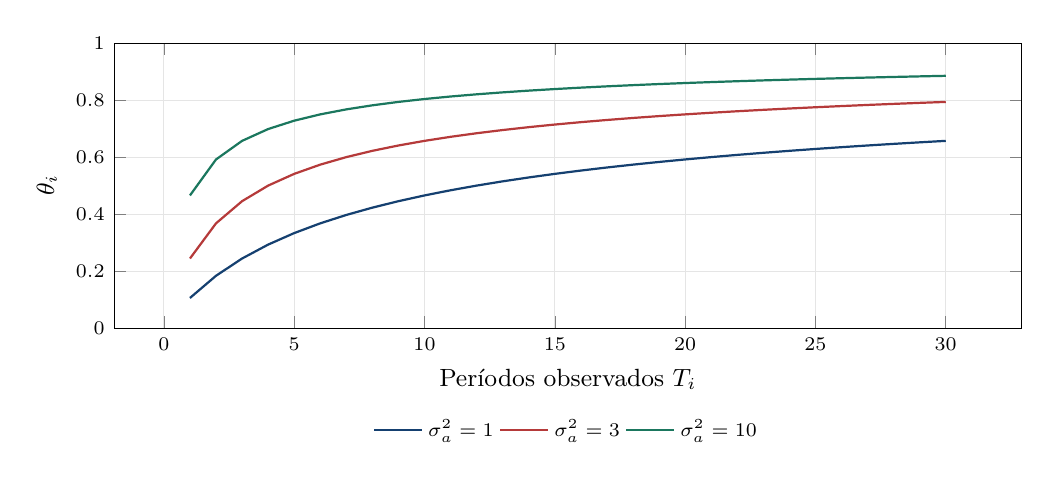
\begin{tikzpicture}
\begin{axis}[panelaxis,xlabel={Períodos observados $T_i$},ylabel={$\theta_i$},ymin=0,ymax=1]
\addplot[azul,thick,no marks] coordinates {(1,0.105572809) (2,0.183503419) (3,0.244071054) (4,0.292893219) (5,0.333333333) (6,0.367544468) (7,0.396977311) (8,0.422649731) (9,0.445299804) (10,0.465477516) (11,0.483602221) (12,0.5) (13,0.51492875) (14,0.528595479) (15,0.541168532) (16,0.552786405) (17,0.56356422) (18,0.573598567) (19,0.582971172) (20,0.59175171) (21,0.6) (22,0.60776773) (23,0.615099821) (24,0.622035527) (25,0.628609324) (26,0.634851628) (27,0.640789396) (28,0.646446609) (29,0.651844688) (30,0.65700283)};
\addlegendentry{$\sigma_a^2=1$}
\addplot[rojo,thick,no marks] coordinates {(1,0.244071054) (2,0.367544468) (3,0.445299804) (4,0.5) (5,0.541168532) (6,0.573598567) (7,0.6) (8,0.622035527) (9,0.640789396) (10,0.65700283) (11,0.671202025) (12,0.683772234) (13,0.695002859) (14,0.705116088) (15,0.714285714) (16,0.722649902) (17,0.730320055) (18,0.737387134) (19,0.74392624) (20,0.75) (21,0.755661111) (22,0.760954278) (23,0.765917706) (24,0.770584266) (25,0.77498242) (26,0.779136948) (27,0.783069542) (28,0.786799284) (29,0.790343033) (30,0.793715751)};
\addlegendentry{$\sigma_a^2=3$}
\addplot[verde,thick,no marks] coordinates {(1,0.465477516) (2,0.59175171) (3,0.65700283) (4,0.698488655) (5,0.727834473) (6,0.75) (7,0.767504723) (8,0.78178211) (9,0.793715751) (10,0.803883865) (11,0.812682838) (12,0.820394698) (13,0.827226315) (14,0.833333333) (15,0.838835407) (16,0.843826238) (17,0.848380391) (18,0.852558044) (19,0.856408368) (20,0.859971992) (21,0.863282815) (22,0.866369379) (23,0.86925591) (24,0.87196312) (25,0.874508839) (26,0.876908509) (27,0.879175581) (28,0.881321834) (29,0.883357631) (30,0.885292133)};
\addlegendentry{$\sigma_a^2=10$}
\end{axis}
\end{tikzpicture}
\caption{Parámetro RE con $\sigma_\eps^2=4$. Más períodos o mayor heterogeneidad permanente dan mayor sustracción de la media individual.}\label{fig:panel-7}
\end{figure}
% FIN PANELFIG
\section{Separación within--between del criterio RE}
Para $r_i=y_i-Z_ib$,
\[
r_i\T\Omega_i^{-1}r_i
=\frac{\sum_t(r_{it}-\bar r_i)^2}{\sigma_\eps^2}
+\frac{T_i\bar r_i^2}{\sigma_\eps^2+T_i\sigma_a^2}.
\]
En panel balanceado con un regresor y tras eliminar el intercepto,
\[
\widehat\beta_{\rm RE}
=\frac{W_{xy}+\kappa B_{xy}}{W_{xx}+\kappa B_{xx}},
\qquad
\kappa=\frac{\sigma_\eps^2}{\sigma_\eps^2+T\sigma_a^2}.
\]
La información entre recibe menor peso cuando aumenta la heterogeneidad. Si las pendientes within y between difieren por confusión, esta combinación eficiente no elimina la confusión.



% PANELFIG 9
\begin{figure}[htbp]\centering
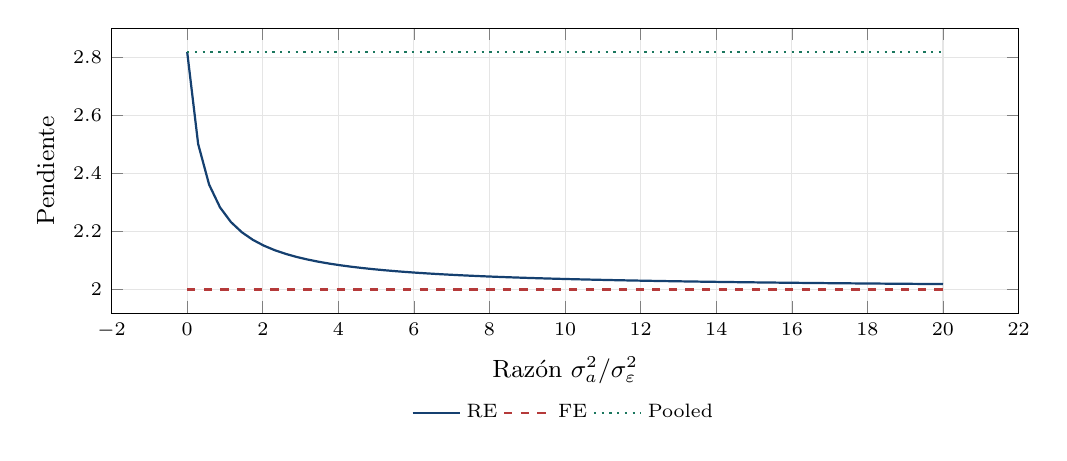
\begin{tikzpicture}
\begin{axis}[panelaxis,xlabel={Razón $\sigma_a^2/\sigma_\eps^2$},ylabel={Pendiente}]
\addplot[azul,thick,no marks] coordinates {(0,2.81818182) (0.289855072,2.50121065) (0.579710145,2.36125654) (0.869565217,2.28240109) (1.15942029,2.23180291) (1.44927536,2.1965812) (1.73913043,2.17065128) (2.02898551,2.15076475) (2.31884058,2.13502935) (2.60869565,2.12226816) (2.89855072,2.11171074) (3.1884058,2.10283159) (3.47826087,2.09526001) (3.76811594,2.08872696) (4.05797101,2.08303249) (4.34782609,2.07802488) (4.63768116,2.07358692) (4.92753623,2.06962664) (5.2173913,2.06607086) (5.50724638,2.06286061) (5.79710145,2.05994787) (6.08695652,2.05729311) (6.37681159,2.0548635) (6.66666667,2.05263158) (6.95652174,2.05057415) (7.24637681,2.04867153) (7.53623188,2.04690687) (7.82608696,2.04526569) (8.11594203,2.04373547) (8.4057971,2.04230533) (8.69565217,2.04096576) (8.98550725,2.03970842) (9.27536232,2.03852596) (9.56521739,2.03741189) (9.85507246,2.03636044) (10.1449275,2.03536648) (10.4347826,2.03442541) (10.7246377,2.03353313) (11.0144928,2.03268593) (11.3043478,2.03188049) (11.5942029,2.03111378) (11.884058,2.03038309) (12.173913,2.02968593) (12.4637681,2.02902005) (12.7536232,2.02838338) (13.0434783,2.02777405) (13.3333333,2.02719033) (13.6231884,2.02663064) (13.9130435,2.02609353) (14.2028986,2.02557766) (14.4927536,2.02508179) (14.7826087,2.02460478) (15.0724638,2.02414557) (15.3623188,2.02370319) (15.6521739,2.02327673) (15.942029,2.02286535) (16.2318841,2.02246825) (16.5217391,2.02208471) (16.8115942,2.02171405) (17.1014493,2.02135562) (17.3913043,2.02100883) (17.6811594,2.02067312) (17.9710145,2.02034798) (18.2608696,2.0200329) (18.5507246,2.01972744) (18.8405797,2.01943115) (19.1304348,2.01914362) (19.4202899,2.01886449) (19.7101449,2.01859337) (20,2.01832994)};
\addlegendentry{RE}
\addplot[rojo,thick,no marks,dashed] coordinates {(0,2) (0.289855072,2) (0.579710145,2) (0.869565217,2) (1.15942029,2) (1.44927536,2) (1.73913043,2) (2.02898551,2) (2.31884058,2) (2.60869565,2) (2.89855072,2) (3.1884058,2) (3.47826087,2) (3.76811594,2) (4.05797101,2) (4.34782609,2) (4.63768116,2) (4.92753623,2) (5.2173913,2) (5.50724638,2) (5.79710145,2) (6.08695652,2) (6.37681159,2) (6.66666667,2) (6.95652174,2) (7.24637681,2) (7.53623188,2) (7.82608696,2) (8.11594203,2) (8.4057971,2) (8.69565217,2) (8.98550725,2) (9.27536232,2) (9.56521739,2) (9.85507246,2) (10.1449275,2) (10.4347826,2) (10.7246377,2) (11.0144928,2) (11.3043478,2) (11.5942029,2) (11.884058,2) (12.173913,2) (12.4637681,2) (12.7536232,2) (13.0434783,2) (13.3333333,2) (13.6231884,2) (13.9130435,2) (14.2028986,2) (14.4927536,2) (14.7826087,2) (15.0724638,2) (15.3623188,2) (15.6521739,2) (15.942029,2) (16.2318841,2) (16.5217391,2) (16.8115942,2) (17.1014493,2) (17.3913043,2) (17.6811594,2) (17.9710145,2) (18.2608696,2) (18.5507246,2) (18.8405797,2) (19.1304348,2) (19.4202899,2) (19.7101449,2) (20,2)};
\addlegendentry{FE}
\addplot[verde,thick,no marks,dotted] coordinates {(0,2.81818182) (0.289855072,2.81818182) (0.579710145,2.81818182) (0.869565217,2.81818182) (1.15942029,2.81818182) (1.44927536,2.81818182) (1.73913043,2.81818182) (2.02898551,2.81818182) (2.31884058,2.81818182) (2.60869565,2.81818182) (2.89855072,2.81818182) (3.1884058,2.81818182) (3.47826087,2.81818182) (3.76811594,2.81818182) (4.05797101,2.81818182) (4.34782609,2.81818182) (4.63768116,2.81818182) (4.92753623,2.81818182) (5.2173913,2.81818182) (5.50724638,2.81818182) (5.79710145,2.81818182) (6.08695652,2.81818182) (6.37681159,2.81818182) (6.66666667,2.81818182) (6.95652174,2.81818182) (7.24637681,2.81818182) (7.53623188,2.81818182) (7.82608696,2.81818182) (8.11594203,2.81818182) (8.4057971,2.81818182) (8.69565217,2.81818182) (8.98550725,2.81818182) (9.27536232,2.81818182) (9.56521739,2.81818182) (9.85507246,2.81818182) (10.1449275,2.81818182) (10.4347826,2.81818182) (10.7246377,2.81818182) (11.0144928,2.81818182) (11.3043478,2.81818182) (11.5942029,2.81818182) (11.884058,2.81818182) (12.173913,2.81818182) (12.4637681,2.81818182) (12.7536232,2.81818182) (13.0434783,2.81818182) (13.3333333,2.81818182) (13.6231884,2.81818182) (13.9130435,2.81818182) (14.2028986,2.81818182) (14.4927536,2.81818182) (14.7826087,2.81818182) (15.0724638,2.81818182) (15.3623188,2.81818182) (15.6521739,2.81818182) (15.942029,2.81818182) (16.2318841,2.81818182) (16.5217391,2.81818182) (16.8115942,2.81818182) (17.1014493,2.81818182) (17.3913043,2.81818182) (17.6811594,2.81818182) (17.9710145,2.81818182) (18.2608696,2.81818182) (18.5507246,2.81818182) (18.8405797,2.81818182) (19.1304348,2.81818182) (19.4202899,2.81818182) (19.7101449,2.81818182) (20,2.81818182)};
\addlegendentry{Pooled}
\end{axis}
\end{tikzpicture}
\caption{Para el panel inicial, RE pasa de pooled hacia within al reducir el peso de la variación entre entidades. Es un cambio de pesos, no una prueba de exogeneidad.}\label{fig:panel-9}
\end{figure}
% FIN PANELFIG
\section{Estimar componentes mediante momentos}
En panel balanceado clásico, FE da
$\widehat\sigma_\eps^2=\mathrm{SSE}_{\rm FE}/[G(T-1)-K]$.
La regresión between de medias tiene $p_B=K+1$ columnas de rango completo y errores de varianza $\sigma_a^2+\sigma_\eps^2/T$. Por ello,
\[
s_B^2=\frac{\mathrm{SSE}_B}{G-p_B},\qquad
\widetilde\sigma_a^2=s_B^2-\widehat\sigma_\eps^2/T.
\]
El segundo puede resultar negativo. La restricción
$\widehat\sigma_a^2=\max(0,\widetilde\sigma_a^2)$ conserva una covarianza admisible, pero introduce sesgo por truncamiento y una masa en cero. No existe una varianza poblacional negativa.

En panel desbalanceado, sea $M_B$ el proyector residual de una regresión between no ponderada. Entonces
\[
\E(\mathrm{SSE}_B\mid X)
=\sigma_a^2\tr(M_B)+
\sigma_\eps^2\tr[M_B\diag(1/T_i)].
\]
Esta identidad permite ajustar momentos. No basta usar un $T$ arbitrario ni sustituir la media de $T_i$ sin derivación; los programas pueden implementar otros estimadores de componentes.

\section{FGLS: propiedades exactas frente a asintóticas}
Si $\widehat\Omega$ se estima con los mismos datos,
\[
\widehat b_{\rm FGLS}
=(Z\T\widehat\Omega^{-1}Z)^{-1}Z\T\widehat\Omega^{-1}y
\]
no es, en general, una transformación lineal determinista de $y$.
No se puede afirmar insesgadez exacta copiando la prueba GLS.
Bajo convergencia de componentes, identificación y muchos grupos independientes, puede ser consistente y tener la misma distribución límite que el GLS apropiado. La matriz $(Z\T\widehat\Omega^{-1}Z)^{-1}$ es una covarianza paramétrica estimada. Una alternativa robusta usa scores por entidad del modelo transformado. Ninguna corrige una media $\E(a_i\mid X_i)$ mal especificada.

\section{Verosimilitud gaussiana y derivadas matriciales}
Con $\psi=(\sigma_\eps^2,\sigma_a^2)$,
\[
\ell(b,\psi)
=-\frac12[n\log(2\pi)+\log|\Omega|+
(y-Zb)\T\Omega^{-1}(y-Zb)].
\]
Para $\psi$ fija, maximizar en $b$ da GLS.
De $\Omega\Omega^{-1}=I$ se obtiene
$\dd\Omega^{-1}=-\Omega^{-1}(\dd\Omega)\Omega^{-1}$.
La derivada del determinante da
$\dd\log|\Omega|=\tr(\Omega^{-1}\dd\Omega)$.
Sea $\Omega_r=\partial\Omega/\partial\psi_r$ y $r=y-Zb$:
\[
\frac{\partial\ell}{\partial\psi_r}
=\frac12[r\T\Omega^{-1}\Omega_r\Omega^{-1}r
-\tr(\Omega^{-1}\Omega_r)].
\]
En el parámetro verdadero ambos términos tienen igual esperanza.
Con media conocida, la información es
\[
\mathcal I_{rs}=\frac12\tr(\Omega^{-1}\Omega_r\Omega^{-1}\Omega_s).
\]
Se impone $\sigma_\eps^2>0$, $\sigma_a^2\ge0$; la frontera requiere tratamiento particular para contrastes.

\section{REML y ajuste por estimar la media}
Una verosimilitud restringida, salvo constantes independientes de $\psi$, es
\[
\ell_R(\psi)=-\frac12[
\log|\Omega|+\log|Z\T\Omega^{-1}Z|+y\T P_\Omega y],
\]
\[
P_\Omega=\Omega^{-1}-\Omega^{-1}Z(Z\T\Omega^{-1}Z)^{-1}Z\T\Omega^{-1}.
\]
$P_\Omega Z=0$ y $P_\Omega\Omega P_\Omega=P_\Omega$.
No es generalmente idempotente en geometría euclídea.
El score de un componente es
$\tfrac12[y\T P_\Omega\Omega_rP_\Omega y-\tr(P_\Omega\Omega_r)]$.
Su esperanza es cero por la anulación del diseño y la identidad anterior.
REML se basa en contrastes que eliminan los efectos de media. No se comparan sin cuidado verosimilitudes REML de modelos con diseños fijos diferentes.

\section{Predecir un intercepto aleatorio y su incertidumbre}
Supongamos $b,\sigma_a^2,\sigma_\eps^2$ conocidos. Sea
$\bar r_i=\bar y_i-c-\bar x_i\T\beta=a_i+\bar\eps_i$.
Por normal conjunta,
\[
\E(a_i\mid y_i,X_i)=\gamma_i\bar r_i,\qquad
\gamma_i=\frac{T_i\sigma_a^2}{\sigma_\eps^2+T_i\sigma_a^2},
\]
\[
\Var(a_i\mid y_i,X_i)=
\frac{\sigma_a^2\sigma_\eps^2}{\sigma_\eps^2+T_i\sigma_a^2}.
\]
$\gamma_i$ contrae hacia cero y no coincide con $\theta_i$:
$\gamma_i=1-(1-\theta_i)^2$.
Con $T_i=2$, $\sigma_a^2=3$, $\sigma_\eps^2=4$, $\gamma_i=0.6$.
Si $\bar r_i=5$, la media posterior es $3$ y la varianza $1.2$.
Al estimar los parámetros existe incertidumbre adicional: la expresión anterior no es toda la varianza de un predictor empírico.



% PANELFIG 8
\begin{figure}[htbp]\centering
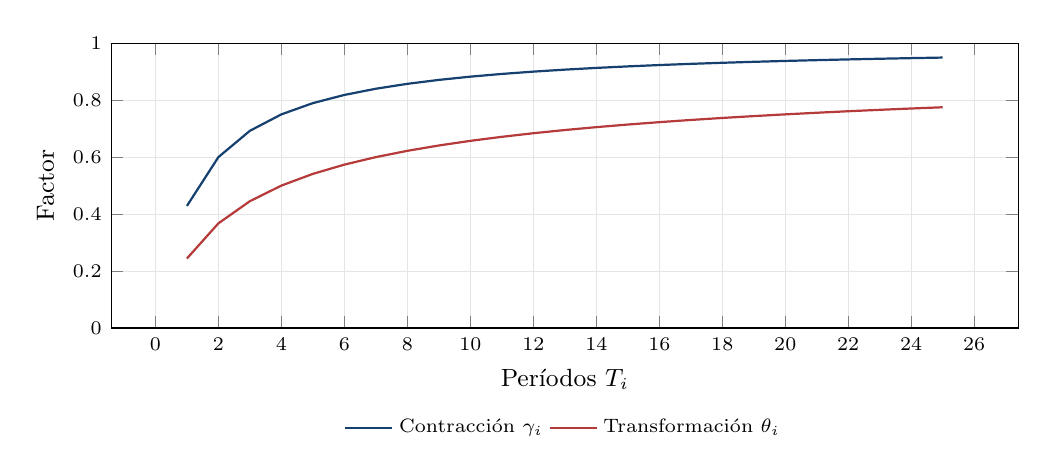
\begin{tikzpicture}
\begin{axis}[panelaxis,xlabel={Períodos $T_i$},ylabel={Factor},ymin=0,ymax=1]
\addplot[azul,thick,no marks] coordinates {(1,0.428571429) (2,0.6) (3,0.692307692) (4,0.75) (5,0.789473684) (6,0.818181818) (7,0.84) (8,0.857142857) (9,0.870967742) (10,0.882352941) (11,0.891891892) (12,0.9) (13,0.906976744) (14,0.913043478) (15,0.918367347) (16,0.923076923) (17,0.927272727) (18,0.931034483) (19,0.93442623) (20,0.9375) (21,0.940298507) (22,0.942857143) (23,0.945205479) (24,0.947368421) (25,0.949367089)};
\addlegendentry{Contracción $\gamma_i$}
\addplot[rojo,thick,no marks] coordinates {(1,0.244071054) (2,0.367544468) (3,0.445299804) (4,0.5) (5,0.541168532) (6,0.573598567) (7,0.6) (8,0.622035527) (9,0.640789396) (10,0.65700283) (11,0.671202025) (12,0.683772234) (13,0.695002859) (14,0.705116088) (15,0.714285714) (16,0.722649902) (17,0.730320055) (18,0.737387134) (19,0.74392624) (20,0.75) (21,0.755661111) (22,0.760954278) (23,0.765917706) (24,0.770584266) (25,0.77498242)};
\addlegendentry{Transformación $\theta_i$}
\end{axis}
\end{tikzpicture}
\caption{La contracción del predictor individual y el parámetro de cuasidesviación son diferentes: $\gamma_i=1-(1-\theta_i)^2$.}\label{fig:panel-8}
\end{figure}
% FIN PANELFIG
\section{Pendientes aleatorias y covarianzas de mayor dimensión}
Un modelo mixto es $y_i=X_ib+R_iu_i+\eps_i$, con $\Var(u_i)=\Sigma_u$.
Entonces $\Omega_i=R_i\Sigma_uR_i\T+\Sigma_{\eps,i}$.
Para intercepto y pendiente aleatorios, $R_i=[\ones,x_i]$ y
\[
\Sigma_u=\begin{pmatrix}\tau_0^2&\tau_{01}\\\tau_{01}&\tau_1^2\end{pmatrix}.
\]
La covarianza entre dos errores compuestos es
$\tau_0^2+\tau_{01}(x_{it}+x_{is})+\tau_1^2x_{it}x_{is}
+\Cov(\eps_{it},\eps_{is})$.
Se requiere $\tau_{01}^2\le\tau_0^2\tau_1^2$. La heterogeneidad de pendientes cambia qué promedio estiman pooled o FE.

\section{Curiosidad: BLUP equivale a una penalización cuadrática}
Minimizar, con parámetros conocidos,
\[
\frac{\norm{y_i-X_ib-R_iu_i}^2}{\sigma_\eps^2}
+u_i\T\Sigma_u^{-1}u_i
\]
da
\[
\widehat u_i=
(R_i\T R_i/\sigma_\eps^2+\Sigma_u^{-1})^{-1}
R_i\T(y_i-X_ib)/\sigma_\eps^2.
\]
La covarianza aleatoria determina cuánto se encoge cada dirección. Bajo normalidad coincide con la media posterior y el predictor lineal óptimo. FE no impone esta penalización sobre los interceptos.



% MODULO 06_twoway_cre.tex
\parte{VI. Dos vías, Mundlak y contrastes de especificación}
\section{Efectos de entidad y tiempo: dos fuentes de confusión}
Ahora $y_{it}=a_i+\lambda_t+x_{it}\T\beta+\eps_{it}$.
Los efectos temporales absorben choques comunes, como inflación o una reforma nacional. No absorben necesariamente choques que afectan de forma distinta a cada entidad.
Sea $F$ la matriz de dummies temporales. El diseño de efectos es $C=[D,F]$ y tiene dependencia porque $D\ones_G=F\ones_T$. Se elimina una columna redundante o se usa una pseudoinversa para construir el proyector único sobre su espacio de columnas.

La pendiente es
\[
\widehat\beta_{\rm TWFE}=(X\T M_CX)^{-1}X\T M_Cy.
\]
Se necesita variación de $X$ que no pueda expresarse como suma de un componente individual y otro temporal. Una variable idéntica para todas las entidades en cada fecha es colineal con $\lambda_t$. Una tendencia $t$ común también lo es si se incluyen dummies de todas las fechas.

\section{Doble centrado en panel balanceado}
Para $G$ entidades y $T$ fechas, definimos
$\bar y_i=T^{-1}\sum_ty_{it}$,
$\bar y_t=G^{-1}\sum_iy_{it}$ y
$\bar y=(GT)^{-1}\sum_i\sum_ty_{it}$.
La transformación de dos vías es
\[
y_{it}^{\circ}=y_{it}-\bar y_i-\bar y_t+\bar y.
\]
Su suma por entidad y por fecha es cero. Con orden entidad--tiempo,
\[
M_C=M_G\otimes M_T,\qquad
M_G=I_G-\ones_G\ones_G\T/G.
\]
Su rango es $(G-1)(T-1)=GT-G-T+1$.
Con $K$ pendientes identificadas, los grados de libertad residuales son
$GT-G-T+1-K$.

\begin{resuelto}{Una tabla de dos por tres}
Sea
\[
Y=\begin{pmatrix}2&4&8\\5&7&10\end{pmatrix}.
\]
Las medias individuales son $14/3$ y $22/3$; las temporales, $7/2,11/2,9$; la global, $6$.
\[
Y^\circ=
\begin{pmatrix}
2-14/3-7/2+6&4-14/3-11/2+6&8-14/3-9+6\\
5-22/3-7/2+6&7-22/3-11/2+6&10-22/3-9+6
\end{pmatrix}
=\begin{pmatrix}-1/6&-1/6&1/3\\1/6&1/6&-1/3\end{pmatrix}.
\]
Cada fila y cada columna suma cero. La transformación deja dos grados de libertad, $(2-1)(3-1)=2$, antes de incluir pendientes.
\end{resuelto}

\section{Por qué el doble centrado simple falla con huecos}
En panel desbalanceado, el promedio temporal se calcula con conjuntos de entidades diferentes. Restar medias individuales puede cambiar las medias temporales y viceversa. Los proyectores $P_D$ y $P_F$ no conmutan en general:
$P_DP_F\ne P_FP_D$.
Por ello $(I-P_F)(I-P_D)$ no es necesariamente el proyector sobre el complemento de ambos espacios.

Un ejemplo de cuatro observaciones es
$\cO=\{(1,1),(1,2),(2,2),(2,3)\}$.
Cada entidad tiene dos filas, pero los tamaños por fecha son $1,2,1$.
Si $y=(1,3,5,7)\T$, restar medias individuales da $(-1,1,-1,1)\T$.
Restar luego medias temporales da $(0,1,-1,0)\T$.
Las medias individuales de ese vector son $1/2$ y $-1/2$: ya no están anuladas. Una sola vuelta no resuelve la proyección conjunta.

\section{Proyecciones alternadas y convergencia}
Empezamos con $v^{(0)}=y$ y repetimos
\[
v^{(m+1)}=(I-P_F)(I-P_D)v^{(m)}.
\]
El límite es la proyección sobre
$\ker(D\T)\cap\ker(F\T)$ en dimensión finita.
La intuición es que cada paso reduce la componente en un espacio de efectos; la norma no aumenta. Las direcciones comunes requieren eliminar redundancias, pero el proyector residual sigue siendo único.

Aplicamos el mismo procedimiento a cada columna de $X$.
Se detiene cuando las medias restantes son menores que una tolerancia escalada y cuando los coeficientes dejan de cambiar a la precisión requerida.
La velocidad depende del ángulo entre espacios: si los patrones de observación conectan débilmente entidades y fechas, la convergencia puede ser lenta. Un método acelerado debe verificarse respecto de la solución de un diseño pequeño explícito.



% PANELFIG 11
\begin{figure}[htbp]\centering
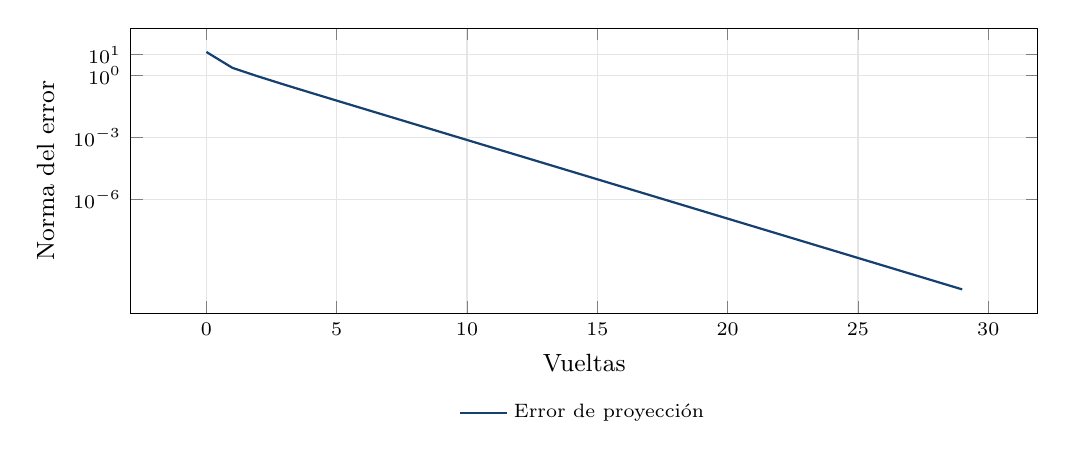
\begin{tikzpicture}
\begin{axis}[panelaxis,xlabel={Vueltas},ylabel={Norma del error},ymode=log,ytick={0.000001,0.001,1,10}]
\addplot[azul,thick,no marks,mark=*] coordinates {(0,13.5769412) (1,2.30940108) (2,0.881917104) (3,0.354642926) (4,0.145796586) (5,0.0604501503) (6,0.025142648) (7,0.010469358) (8,0.00436122023) (9,0.00181702324) (10,0.000757070234) (11,0.000315442514) (12,0.000131433868) (13,5.47640348e-05) (14,2.28183363e-05) (15,9.5076384e-06) (16,3.96151574e-06) (17,1.65063152e-06) (18,6.87763128e-07) (19,2.86567969e-07) (20,1.1940332e-07) (21,4.97513834e-08) (22,2.0729743e-08) (23,8.6373928e-09) (24,3.59891361e-09) (25,1.49954726e-09) (26,6.24811314e-10) (27,2.60337973e-10) (28,1.08474119e-10) (29,4.51975124e-11)};
\addlegendentry{Error de proyección}
\end{axis}
\end{tikzpicture}
\caption{Convergencia en un panel sintético desbalanceado de siete filas. La referencia se calcula con el diseño conjunto; una sola vuelta no basta.}\label{fig:panel-11}
\end{figure}
% FIN PANELFIG
\section{Conectividad y rango de los efectos fijos}
Construimos un grafo bipartito: un nodo por entidad, otro por fecha y una arista por observación. Si tiene $c$ componentes conexas y todas las entidades y fechas listadas aparecen al menos una vez, el rango de $[D,F]$ es
\[
\rank([D,F])=G+T-c.
\]
\begin{deduccion}
Una combinación $Da+F\lambda=0$ exige $a_i+\lambda_t=0$ en cada arista. Dentro de una componente conexa, todos los $a_i$ deben compartir una constante y todos los $\lambda_t$ su opuesto. Cada componente aporta exactamente una dirección redundante; hay $c$ en total.
\end{deduccion}
Así los grados de libertad residuales, con $K$ pendientes adicionales independientes, son
$n-G-T+c-K$. Un panel con huecos no debe recibir automáticamente el divisor del panel balanceado.

\section{Mundlak: representar la correlación con los regresores}
Supongamos
\[
a_i=\bar x_i\T\pi+r_i,\qquad
\E(r_i\mid X_i)=0.
\]
Al sustituir,
$y_{it}=c+x_{it}\T\beta+\bar x_i\T\pi+r_i+\eps_{it}$.
Este modelo de efectos aleatorios correlacionados, CRE, incluye las medias individuales de los regresores que varían en el tiempo.
La hipótesis $\pi=0$ expresa una restricción RE de media dentro de esta representación; no demuestra toda posible independencia distribucional.

Podemos escribir
\[
x_{it}\T\beta+\bar x_i\T\pi
=(x_{it}-\bar x_i)\T\beta+\bar x_i\T(\beta+\pi).
\]
El coeficiente within es $\beta$ y el between es $\beta+\pi$.
En el modelo lineal clásico, incluir todas las medias correspondientes permite reproducir las pendientes FE de los regresores temporales mediante la separación ortogonal de bloques.
Variables invariantes pueden incorporarse, pero sus coeficientes aún requieren restricciones sobre la heterogeneidad residual: CRE no identifica automáticamente sus efectos causales.

\section{La equivalencia FE--CRE mediante ortogonalidad}
Con componentes RE clásicos, el criterio se separa en:
\[
\sum_i\frac{\norm{M_i(y_i-X_i\beta)}^2}{\sigma_\eps^2}
+\sum_i\frac{T_i(\bar y_i-c-\bar x_i\T(\beta+\pi))^2}
{\sigma_\eps^2+T_i\sigma_a^2}.
\]
Definimos $\eta=\beta+\pi$.
El primer término depende únicamente de $\beta$; el segundo, de $c,\eta$.
Al permitir $\pi$ libre, $\beta$ queda determinada por el primer término y coincide con FE. Esto exige la especificación completa y el mismo conjunto de observaciones. Con restricciones sobre las medias, pesos distintos o variables omitidas, la equivalencia puede desaparecer.

\section{El contraste F de interceptos comunes}
Comparamos un modelo pooled restringido con un modelo FE no restringido.
Sea $\mathrm{SSE}_R$ la suma de cuadrados pooled, $\mathrm{SSE}_U$ la FE.
Si ambos usan las mismas filas, tienen $K$ pendientes y el modelo completo rango $G+K$,
\[
F=\frac{(\mathrm{SSE}_R-\mathrm{SSE}_U)/(G-1)}
{\mathrm{SSE}_U/(n-G-K)}.
\]
Bajo errores normales esféricos y la hipótesis de interceptos iguales,
$F\sim F_{G-1,n-G-K}$ exactamente.
La diferencia de sumas de cuadrados es no negativa porque los espacios están anidados.
Con dependencia por entidad, este F clásico no es robusto. Probar muchas dummies con pocos grupos requiere inferencia compatible con la dependencia.

\section{Hausman: deducir la covarianza de una diferencia}
Supongamos que bajo una hipótesis nula dos estimadores son consistentes:
$\widehat\beta_F$ y $\widehat\beta_R$, y que $\widehat\beta_R$ es eficiente en la clase pertinente.
La propiedad de eficiencia bajo esa nula implica, en el régimen asintótico apropiado,
$\Cov(\widehat\beta_F,\widehat\beta_R)=V_R$.
Así, para $d=\widehat\beta_F-\widehat\beta_R$,
\[
\Var(d)=V_F+V_R-\Cov(F,R)-\Cov(R,F)=V_F-V_R.
\]
El estadístico $H=d\T(V_F-V_R)^{-1}d$ es asintóticamente chi-cuadrado con el rango de las restricciones identificadas, si la matriz tiene las propiedades requeridas.

No es una identidad para cualquier par de matrices robustas. Restar dos covarianzas calculadas por métodos distintos puede producir una matriz indefinida. Un $H$ negativo indica que el cálculo no corresponde a una forma cuadrática positiva válida, no una evidencia especial a favor de RE. Se puede utilizar una prueba robusta de medias Mundlak o una covarianza conjunta bien estimada de la diferencia.

\begin{resuelto}{Hausman escalar y una alternativa matricial}
Si $\widehat\beta_F=0.8$, $\widehat\beta_R=0.5$, $V_F=0.09$, $V_R=0.04$ y las condiciones justifican su diferencia,
$H=(0.8-0.5)^2/(0.09-0.04)=1.8$.
Si las varianzas robustas fueran $0.03$ y $0.04$, el denominador sería negativo y esa fórmula no define un contraste válido.
Para dos pendientes, si
\[
d=\begin{pmatrix}1/5\\-1/10\end{pmatrix},
\quad
V_d=\begin{pmatrix}1/10&1/50\\1/50&1/20\end{pmatrix},
\]
se usa la inversa completa. El término cruzado de $d\T V_d^{-1}d$ importa; sumar dos cocientes diagonalmente ignora la correlación entre diferencias.
\end{resuelto}

\section{Prueba de componente aleatorio y la frontera}
La hipótesis $\sigma_a^2=0$ está en la frontera de $\sigma_a^2\ge0$.
En un panel balanceado clásico, un LM de dos lados frecuentemente escrito para la estructura de componentes usa residuos pooled:
\[
LM=\frac{GT}{2(T-1)}
\left[
\frac{\sum_i(\sum_t\widehat v_{it})^2}
{\sum_i\sum_t\widehat v_{it}^2}-1
\right]^2.
\]
Su calibración habitual como chi-cuadrado de un grado y las versiones unilaterales tienen hipótesis y convenciones distintas. Para una prueba restringida de un componente no negativo, pueden aparecer mezclas de distribuciones en la frontera; no se debe equiparar toda implementación de LM con un LRT unilateral.
La expresión revela el objeto medido: sumas de residuos por entidad mayores que lo esperado bajo ausencia de covarianza temporal. Otros procesos seriales pueden generar ese patrón sin un intercepto aleatorio clásico.

\section{Curiosidad: seleccionar un modelo con un test también es aleatorio}
Elegir FE si un test rechaza y RE si no rechaza crea un estimador compuesto.
Su distribución no coincide sin más con la del modelo seleccionado como si hubiera sido prefijado.
No rechazar correlación no demuestra correlación cero; una prueba con poca potencia puede favorecer por azar una restricción falsa.
La elección debe apoyarse en el diseño, el significado de las variables y las condiciones de identificación, usando los contrastes como información complementaria.



% MODULO 07_inferencia.tex
\parte{VII. Inferencia con heterocedasticidad y dependencia}
\section{El error verdadero no es el residuo estimado}
El error $\eps_{it}$ pertenece a la ecuación poblacional; el residuo $\widehat\eps_{it}$ se calcula después de ajustar coeficientes. Para el modelo FE,
$\widehat\eps=M_{[D,X]}\eps$.
Sus varianzas y covarianzas son distintas de las de $\eps$.
Las restricciones de suma cero y de ortogonalidad imponen dependencia a los residuos. Por eso una matriz construida con ellos estima la covarianza de los errores solo bajo condiciones y, a menudo, en un límite de muestra grande.

Heterocedasticidad significa que las varianzas difieren. Autocorrelación significa dependencia temporal dentro de una entidad. Dependencia transversal significa que errores de entidades diferentes están correlacionados.
Estos son tres problemas diferentes; agrupar por entidad protege frente a dependencia dentro de entidad, pero no frente a cualquier choque compartido entre entidades.

\section{La matriz sandwich derivada por entidades}
Sea $\widetilde X_i=M_iX_i$, $\widetilde\eps_i=M_i\eps_i$ y
$Q=\sum_i\widetilde X_i\T\widetilde X_i$.
Entonces
\[
\widehat\beta-\beta=Q^{-1}\sum_i s_i,\qquad
s_i=\widetilde X_i\T\widetilde\eps_i.
\]
Si las entidades son independientes,
\[
\Var\left(\sum_i s_i\mid X\right)=\sum_i\Var(s_i\mid X).
\]
Reemplazando cada score verdadero por
$\widehat s_i=\widetilde X_i\T\widehat\eps_i$,
\[
\widehat V_{\rm CR0}
=Q^{-1}\left(\sum_{i=1}^G\widehat s_i\widehat s_i\T\right)Q^{-1}.
\]
Es la covarianza agrupada sin corrección finita. Conserva todos los productos temporales dentro de cada entidad, incluidos términos fuera de diagonal:
\[
\widehat s_{i,k}\widehat s_{i,\ell}
=\sum_{t\in\mathcal T_i}\sum_{r\in\mathcal T_i}
\widetilde x_{it,k}\widetilde x_{ir,\ell}
\widehat\eps_{it}\widehat\eps_{ir}.
\]
El estimador heterocedástico por filas conserva solamente términos $t=r$ y no permite en general dependencia temporal.

\section{Todas las entradas de una sandwich de dos pendientes}
Con
$Q^{-1}=\begin{pmatrix}a&b\\b&d\end{pmatrix}$ y
$S=\sum_i\widehat s_i\widehat s_i\T=
\begin{pmatrix}s_{11}&s_{12}\\s_{12}&s_{22}\end{pmatrix}$,
\[
\begin{aligned}
\widehat V_{11}&=a^2s_{11}+2abs_{12}+b^2s_{22},\\
\widehat V_{22}&=b^2s_{11}+2bds_{12}+d^2s_{22},\\
\widehat V_{12}&=abs_{11}+(ad+b^2)s_{12}+bds_{22}.
\end{aligned}
\]
El error estándar de una pendiente es la raíz de una diagonal. La varianza de su suma es $V_{11}+V_{22}+2V_{12}$.
Si un score es negativo, su cuadrado sigue siendo positivo; scores de dos columnas con signos opuestos aportan covarianzas negativas.

\section{Normalidad límite con muchos conglomerados}
Para $T$ acotado y $G\to\infty$, definimos
\[
Q_G=\frac1G\sum_i\widetilde X_i\T\widetilde X_i,\quad
S_G=\frac1G\sum_i\E(s_is_i\T).
\]
Si $Q_G\to Q_0$ invertible, los scores son de media cero, hay momentos suficientes y ningún grupo domina, una ley de grandes números y un teorema central del límite dan
\[
\sqrt G(\widehat\beta-\beta)
\ \overset d\longrightarrow\
N(0,Q_0^{-1}S_0Q_0^{-1}).
\]
Las condiciones concretas sobre dependencia, colas y tamaños de grupos son parte del teorema que se aplica. No se deduce este límite solo de que $n$ sea grande. Con $G$ fijo y $T\to\infty$ se necesita otra teoría temporal.

La normalidad de cada error individual no es necesaria para esta aproximación.
Pero si un conglomerado concentra casi toda la variación de una variable de política, puede fallar la aproximación de muchos scores pequeños.

\section{Correcciones finitas y grados de libertad}
Una corrección CR1 multiplica CR0 por un factor como
\[
c=\frac G{G-1}\frac{n-1}{n-p},
\]
donde el conteo de $p$ depende del modelo y de la convención del programa, especialmente con efectos absorbidos y anidamiento.
No hay una única corrección universal; no se debe copiar un $p$ incompatible con el ajuste.

Usar Student con $G-1$ grados suele ser una aproximación práctica, no una distribución exacta bajo correlación arbitraria.
CR2 ajusta residuos mediante matrices relacionadas con el apalancamiento y un modelo de trabajo, intentando reducir el sesgo de la covarianza.
Puede acompañarse de grados de libertad tipo Satterthwaite específicos para cada contraste.
Una corrección escalar de CR1 no reproduce esos ajustes matriciales.

\section{Apalancamiento y el motivo de HC2 o HC3}
En MCO clásico, $h_{jj}=[P_Z]_{jj}$ y
$\E(\widehat u_j^2\mid Z)=\sigma^2(1-h_{jj})$.
Esto motiva HC2 con $\widehat u_j^2/(1-h_{jj})$.
HC3 utiliza $\widehat u_j^2/(1-h_{jj})^2$, relacionado con residuos al eliminar la observación:
$\widehat u_{j,(-j)}=\widehat u_j/(1-h_{jj})$.
Estas correcciones por fila no convierten observaciones dependientes en independientes.
A nivel de conglomerado hay bloques de apalancamiento, no solo diagonales.

\section{Dos vías de agrupación e inclusión--exclusión}
Si la dependencia puede aparecer entre filas que comparten entidad o fecha, construimos scores por entidad $s_i$, por fecha $q_t$ y por intersección entidad--fecha $r_{it}$.
La matriz meat de dos vías es
\[
\widehat S_{2w}
=\sum_i s_is_i\T+\sum_tq_tq_t\T-\sum_{(i,t)\in\cO}r_{it}r_{it}\T.
\]
Se resta la intersección porque fue contada dos veces. Si hay varias filas por celda, el score de intersección suma esas filas; no se sustituye automáticamente por HC por observación.

La consistencia requiere un régimen que permita suficiente información en ambas dimensiones y condiciones sobre dependencia y grupos dominantes.
Con muchas entidades y muy pocas fechas, la segunda dimensión sigue siendo pequeña. La inclusión--exclusión puede producir una matriz estimada indefinida en muestras pequeñas; no es una prueba de que la covarianza verdadera sea indefinida.

\section{HAC temporal y Driscoll--Kraay}
Para ilustrar HAC con $T$ grande, agregamos por fecha
$g_t=\sum_i\widetilde x_{it}\widehat\eps_{it}$.
Un meat sin normalización adicional, compatible con $Q$ expresado como suma, es
\[
\widehat S_{\rm HAC}
=\sum_{t=1}^Tg_tg_t\T+
\sum_{\ell=1}^L w_\ell
\sum_{t=\ell+1}^T
(g_tg_{t-\ell}\T+g_{t-\ell}g_t\T),
\]
con pesos Bartlett $w_\ell=1-\ell/(L+1)$.
La covarianza es $Q^{-1}\widehat S_{\rm HAC}Q^{-1}$.
Si se definen los $g_t$ como promedios, deben ajustarse también los factores de escala.

Esta construcción permite correlación entre entidades dentro de una fecha mediante la agregación y autocorrelación de esos scores en el tiempo.
La justificación de Driscoll--Kraay depende de una dimensión temporal suficientemente grande y restricciones de dependencia y momentos; no es una solución automática para $T=3$. Elegir el ancho de banda $L$ implica equilibrar sesgo y varianza.

\section{Autocorrelación AR(1) y sus transformaciones}
Si $\eps_{it}=\rho\eps_{i,t-1}+\eta_{it}$, $|\rho|<1$, y el proceso es estacionario,
\[
\Var(\eps_{it})=\frac{\sigma_\eta^2}{1-\rho^2},
\qquad
\Cov(\eps_{it},\eps_{is})=
\frac{\sigma_\eta^2}{1-\rho^2}\rho^{|t-s|}.
\]
Para $\rho$ conocido, la transformación
$\eps_{it}-\rho\eps_{i,t-1}=\eta_{it}$ blanquea las filas posteriores.
La primera fila estacionaria se escala por $\sqrt{1-\rho^2}$.
Si además hay un intercepto individual,
$y_{it}-\rho y_{i,t-1}=(1-\rho)a_i+
(x_{it}-\rho x_{i,t-1})\T\beta+\eta_{it}$.
El efecto individual no desaparece; debe tratarse también. Diferenciar y cuasidiferenciar cumplen funciones distintas.



% PANELFIG 12
\begin{figure}[htbp]\centering
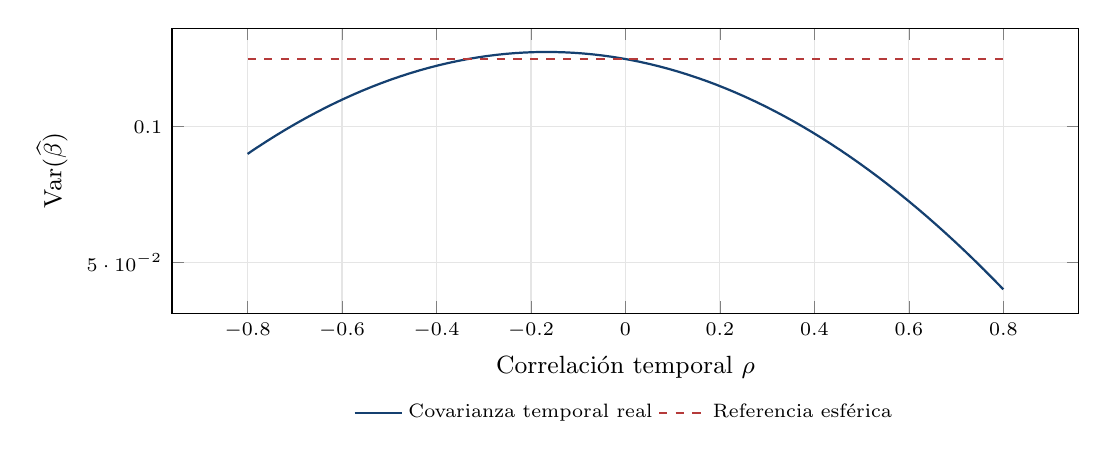
\begin{tikzpicture}
\begin{axis}[panelaxis,xlabel={Correlación temporal $\rho$},ylabel={$\Var(\widehat\beta)$}]
\addplot[azul,thick,no marks] coordinates {(-0.8,0.09) (-0.779746835,0.0923666079) (-0.759493671,0.0946563051) (-0.739240506,0.0968690915) (-0.718987342,0.0990049672) (-0.698734177,0.101063932) (-0.678481013,0.103045986) (-0.658227848,0.10495113) (-0.637974684,0.106779362) (-0.617721519,0.108530684) (-0.597468354,0.110205095) (-0.57721519,0.111802596) (-0.556962025,0.113323185) (-0.536708861,0.114766864) (-0.516455696,0.116133632) (-0.496202532,0.11742349) (-0.475949367,0.118636436) (-0.455696203,0.119772472) (-0.435443038,0.120831598) (-0.415189873,0.121813812) (-0.394936709,0.122719116) (-0.374683544,0.123547508) (-0.35443038,0.124298991) (-0.334177215,0.124973562) (-0.313924051,0.125571223) (-0.293670886,0.126091972) (-0.273417722,0.126535812) (-0.253164557,0.12690274) (-0.232911392,0.127192758) (-0.212658228,0.127405864) (-0.192405063,0.127542061) (-0.172151899,0.127601346) (-0.151898734,0.127583721) (-0.13164557,0.127489184) (-0.111392405,0.127317738) (-0.0911392405,0.12706938) (-0.0708860759,0.126744112) (-0.0506329114,0.126341932) (-0.0303797468,0.125862842) (-0.0101265823,0.125306842) (0.0101265823,0.12467393) (0.0303797468,0.123964108) (0.0506329114,0.123177375) (0.0708860759,0.122313732) (0.0911392405,0.121373177) (0.111392405,0.120355712) (0.13164557,0.119261336) (0.151898734,0.11809005) (0.172151899,0.116841852) (0.192405063,0.115516744) (0.212658228,0.114114725) (0.232911392,0.112635796) (0.253164557,0.111079955) (0.273417722,0.109447204) (0.293670886,0.107737542) (0.313924051,0.105950969) (0.334177215,0.104087486) (0.35443038,0.102147092) (0.374683544,0.100129787) (0.394936709,0.0980355712) (0.415189873,0.0958644448) (0.435443038,0.0936164076) (0.455696203,0.0912914597) (0.475949367,0.088889601) (0.496202532,0.0864108316) (0.516455696,0.0838551514) (0.536708861,0.0812225605) (0.556962025,0.0785130588) (0.57721519,0.0757266464) (0.597468354,0.0728633232) (0.617721519,0.0699230892) (0.637974684,0.0669059446) (0.658227848,0.0638118891) (0.678481013,0.0606409229) (0.698734177,0.057393046) (0.718987342,0.0540682583) (0.739240506,0.0506665598) (0.759493671,0.0471879506) (0.779746835,0.0436324307) (0.8,0.04)};
\addlegendentry{Covarianza temporal real}
\addplot[rojo,thick,no marks,dashed] coordinates {(-0.8,0.125) (-0.779746835,0.125) (-0.759493671,0.125) (-0.739240506,0.125) (-0.718987342,0.125) (-0.698734177,0.125) (-0.678481013,0.125) (-0.658227848,0.125) (-0.637974684,0.125) (-0.617721519,0.125) (-0.597468354,0.125) (-0.57721519,0.125) (-0.556962025,0.125) (-0.536708861,0.125) (-0.516455696,0.125) (-0.496202532,0.125) (-0.475949367,0.125) (-0.455696203,0.125) (-0.435443038,0.125) (-0.415189873,0.125) (-0.394936709,0.125) (-0.374683544,0.125) (-0.35443038,0.125) (-0.334177215,0.125) (-0.313924051,0.125) (-0.293670886,0.125) (-0.273417722,0.125) (-0.253164557,0.125) (-0.232911392,0.125) (-0.212658228,0.125) (-0.192405063,0.125) (-0.172151899,0.125) (-0.151898734,0.125) (-0.13164557,0.125) (-0.111392405,0.125) (-0.0911392405,0.125) (-0.0708860759,0.125) (-0.0506329114,0.125) (-0.0303797468,0.125) (-0.0101265823,0.125) (0.0101265823,0.125) (0.0303797468,0.125) (0.0506329114,0.125) (0.0708860759,0.125) (0.0911392405,0.125) (0.111392405,0.125) (0.13164557,0.125) (0.151898734,0.125) (0.172151899,0.125) (0.192405063,0.125) (0.212658228,0.125) (0.232911392,0.125) (0.253164557,0.125) (0.273417722,0.125) (0.293670886,0.125) (0.313924051,0.125) (0.334177215,0.125) (0.35443038,0.125) (0.374683544,0.125) (0.394936709,0.125) (0.415189873,0.125) (0.435443038,0.125) (0.455696203,0.125) (0.475949367,0.125) (0.496202532,0.125) (0.516455696,0.125) (0.536708861,0.125) (0.556962025,0.125) (0.57721519,0.125) (0.597468354,0.125) (0.617721519,0.125) (0.637974684,0.125) (0.658227848,0.125) (0.678481013,0.125) (0.698734177,0.125) (0.718987342,0.125) (0.739240506,0.125) (0.759493671,0.125) (0.779746835,0.125) (0.8,0.125)};
\addlegendentry{Referencia esférica}
\end{axis}
\end{tikzpicture}
\caption{La varianza FE depende de la orientación de los regresores respecto del proceso de errores. Una correlación positiva no aumenta necesariamente toda varianza de toda pendiente.}\label{fig:panel-12}
\end{figure}
% FIN PANELFIG
\section{Bootstrap por grupos y wild cluster bootstrap}
En bootstrap por entidades se remuestrean trayectorias completas, conservando sus filas internas. Es apropiado para diseños donde las entidades son unidades de muestreo independientes y el número de ellas es suficiente. Remuestrear filas rompe la dependencia temporal.

Un wild cluster bootstrap asigna un peso $w_i$ a todos los residuos de una entidad y genera
$y_i^*=\widehat y_i^{\,R}+w_i\widehat u_i^{\,R}$ en una implementación restringida bajo la nula.
Se vuelve a estimar y se forma un estadístico studentizado. Los pesos Rademacher toman $\pm1$ con igual probabilidad; otras elecciones y ajustes se usan según el diseño.
La versión restringida impone la hipótesis que se desea contrastar.
Con muy pocos grupos, tratamientos concentrados o apalancamiento extremo, no existe una garantía universal de buena calibración.

\section{Un contraste de varias pendientes y una región elíptica}
Para $R\beta=r$ con $q$ restricciones,
\[
W=(R\widehat\beta-r)\T
(R\widehat V R\T)^{-1}(R\widehat\beta-r).
\]
Bajo una teoría asintótica válida, $W$ se aproxima a $\chi_q^2$.
En el modelo normal esférico con varianza residual, un F exacto usa la covarianza y los grados de libertad apropiados.
Para dos pendientes, la región conjunta es una elipse
$(b-\widehat\beta)\T\widehat V^{-1}(b-\widehat\beta)\le c$.
Dos intervalos marginales al 95\% no forman por sí solos una región conjunta al 95\%.

\section{Curiosidad: agrupar cambia la incertidumbre, no la pendiente}
Con el mismo objetivo MCO y las mismas filas, cambiar entre una covarianza clásica y una agrupada no cambia $\widehat\beta$.
Modifica errores estándar, estadísticos e intervalos. En cambio, aplicar GLS o cambiar pesos altera la función objetivo y puede cambiar la pendiente.
Esta separación evita interpretar una reducción del error estándar como un nuevo efecto estimado.

\section{Diagnóstico que corresponde a cada supuesto}
Un gráfico de residuos por tiempo puede revelar patrones, pero no demostrar exogeneidad.
Un test de serialidad investiga dependencia del error; un test de medias Mundlak investiga una restricción de correlación con heterogeneidad; un contraste de rango investiga identificación.
Una prueba de pretrends en DID se refiere a una implicación del diseño causal.
Cada herramienta responde a una pregunta; ninguna certifica todas las condiciones del panel.



% MODULO 08_iv_gmm.tex
\parte{VIII. Instrumentos en panel: eliminar un efecto no elimina toda endogeneidad}
\section{La endogeneidad después de within}
Si $y_{it}=a_i+x_{it}\beta+\eps_{it}$ y $x_{it}$ responde al mismo choque $\eps_{it}$, restar $a_i$ no elimina $\Cov(x_{it},\eps_{it})$.
FE controla heterogeneidad permanente, pero no decisiones simultáneas, anticipación, errores de medición o choques omitidos temporales.
Un instrumento $z_{it}$ necesita relevancia para el regresor transformado y exogeneidad para el error transformado.

Sea $\widetilde y=M_Dy$, $\widetilde X=M_DX$ y $\widetilde Z=M_DZ$. La condición
$\E(Z_i\T M_i\eps_i)=0$ es central. Una condición suficiente es exogeneidad estricta del instrumento respecto de la trayectoria de errores.
Un instrumento invariante en el tiempo queda anulado por $M_D$ y no identifica una pendiente FE mediante la transformación ordinaria.

\section{2SLS: dos proyecciones y una sola fórmula}
Sea $P_{\widetilde Z}=\widetilde Z(\widetilde Z\T\widetilde Z)^{-1}\widetilde Z\T$, usando un conjunto de instrumentos de rango completo.
Primera etapa: $\widehat X=P_{\widetilde Z}\widetilde X$.
Segunda etapa:
\[
\widehat\beta_{\rm IV}
=(\widetilde X\T P_{\widetilde Z}\widetilde X)^{-1}
\widetilde X\T P_{\widetilde Z}\widetilde y.
\]
Como $P_{\widetilde Z}$ es simétrico e idempotente,
$\widehat X\T\widehat X=\widetilde X\T P_{\widetilde Z}\widetilde X$.
La identificación requiere rango $K$ en la relación entre instrumentos y regresores, no solo muchas columnas en $Z$.

Con un regresor y un instrumento,
\[
\widehat\beta_{\rm IV}
=\frac{\sum_i\sum_t\widetilde z_{it}\widetilde y_{it}}
{\sum_i\sum_t\widetilde z_{it}\widetilde x_{it}}
=\beta+
\frac{\sum_i\sum_t\widetilde z_{it}\widetilde\eps_{it}}
{\sum_i\sum_t\widetilde z_{it}\widetilde x_{it}}.
\]
El denominador aleatorio es la fuente de dificultades que MCO de diseño fijo no comparte.

\section{La esperanza de IV no es automáticamente el coeficiente}
La condición $\E(Z\T\eps)=0$ no implica
\[
\E\left[\frac{Z\T\eps}{Z\T X}\right]=0.
\]
El numerador puede estar correlacionado con el inverso del denominador; el cociente incluso puede carecer de esperanza absoluta. En instrumentos débiles, valores de $Z\T X$ próximos a cero pueden producir colas muy pesadas.
Por tanto, no se da una fórmula universal de media y varianza finitas de IV.

Una afirmación exacta distinta sí puede hacerse si se condiciona en $(X,Z)$ y se impone $\E(\eps\mid X,Z)=0$:
el estimador es entonces lineal en $y$ para ese diseño y es condicionalmente insesgado. Esa condición es mucho más fuerte que la validez ordinaria de instrumentos y elimina la endogeneidad condicional que motiva IV.

\section{La covarianza de una transformación IV con diseño fijo}
Definimos
\[
A_{\rm IV}=(\widetilde X\T P_{\widetilde Z}\widetilde X)^{-1}
\widetilde X\T P_{\widetilde Z}M_D.
\]
Con matrices fijas y covarianza $\Omega$ del error original,
\[
\Var(\widehat\beta_{\rm IV}\mid X,Z)=A_{\rm IV}\Omega A_{\rm IV}\T.
\]
Si $\Omega=\sigma^2I$ y $P_{\widetilde Z}M_D=P_{\widetilde Z}$,
\[
\Var(\widehat\beta_{\rm IV}\mid X,Z)
=\sigma^2(\widetilde X\T P_{\widetilde Z}\widetilde X)^{-1}.
\]
La media condicional todavía depende de $\E(\eps\mid X,Z)$.
Esta es una identidad de covarianza de una transformación, no un teorema de insesgadez bajo la validez instrumental débil.

\section{GMM desde condiciones de momento}
Sea $g_i(\beta)=Z_i\T(y_i^*-X_i^*\beta)\in\R^L$, donde la transformación $*$ puede ser within, diferencias u otra que corresponda.
El momento muestral es $\bar g_G(\beta)=G^{-1}\sum_i g_i(\beta)$.
Minimizamos
\[
J_G(\beta)=G\,\bar g_G(\beta)\T W_G\bar g_G(\beta),
\]
con $W_G$ simétrica definida positiva.
Definimos $D_G=G^{-1}\sum_i Z_i\T X_i^*$ y
$h_G=G^{-1}\sum_iZ_i\T y_i^*$.
La solución lineal es
\[
\widehat\beta_W=(D_G\T W_GD_G)^{-1}D_G\T W_Gh_G.
\]
Si $L=K$ y $D_G$ invertible, la solución satisface $\bar g_G=0$ independientemente de $W_G$. Si $L>K$, distintos pesos pueden producir distintos estimadores.

\section{Distribución límite y covarianzas de GMM}
Supongamos $\E[g_i(\beta_0)]=0$, identificación, muchos grupos independientes y momentos suficientes. Sea
$D=\plim D_G$ y $S=\lim G^{-1}\sum_i\E[g_i(\beta_0)g_i(\beta_0)\T]$.
Entonces
\[
\sqrt G(\widehat\beta_W-\beta_0)\overset d\longrightarrow
N(0,V_W),
\]
\[
V_W=(D\T WD)^{-1}D\T WSWD(D\T WD)^{-1}.
\]
La covarianza del estimador, en escala original, se aproxima por $V_W/G$.
Con $W=S^{-1}$,
$V_{\rm ef}=(D\T S^{-1}D)^{-1}$.
Cada entrada da una varianza o covarianza asintótica. En dos etapas se estima $S$ con residuos de una primera etapa. La matriz asintótica plug-in puede subestimar la variabilidad en muestras pequeñas; existen correcciones específicas para GMM de dos etapas.

\section{Prueba J y el significado limitado de no rechazar}
Si hay $L-K$ restricciones sobreidentificadoras independientes y el peso es consistente para $S^{-1}$,
\[
J=G\,\bar g_G(\widehat\beta)\T\widehat S^{-1}\bar g_G(\widehat\beta)
\overset d\longrightarrow\chi_{L-K}^2.
\]
La prueba investiga el conjunto de momentos con la especificación del modelo.
No identifica qué instrumento es inválido si rechaza.
No rechazar no demuestra validez; con muchos instrumentos, la prueba puede perder utilidad.
En una identificación exacta $L=K$, los momentos se anulan y no hay restricciones sobrantes que contrastar.

\section{Instrumentos débiles y contraste Anderson--Rubin}
Para probar $\beta=\beta_0$, se transforma el resultado:
$y^*-X^*\beta_0$.
Bajo la nula y exogeneidad instrumental, no debería ser explicado por instrumentos excluidos, condicionado en los controles.
Un contraste de esos coeficientes puede construirse con una covarianza agrupada válida. Se invierte el conjunto de valores $\beta_0$ que no se rechazan para formar una región robusta a identificación débil, bajo las condiciones del contraste.

El conjunto puede ser amplio, disjunto o no acotado. Eso refleja escasa información; forzarlo a un intervalo corto genera una certeza artificial.
Un F grande de primera etapa es un diagnóstico, pero sus umbrales dependen de la estructura de instrumentos, heterocedasticidad y dependencia. No existe un número mágico universal para todos los paneles.

\section{Errores de segunda etapa: usar el residuo estructural}
La regresión de $y^*$ sobre $\widehat X$ da la pendiente 2SLS, pero su residuo de ajuste
$y^*-\widehat X\widehat\beta$ no es el residuo estructural
$y^*-X^*\widehat\beta$.
El estimador de covarianza IV debe usar el segundo en sus momentos.
La fórmula de MCO reportada por una segunda regresión manual trata $\widehat X$ como regresores observados sin incorporar el problema instrumental y puede ser incorrecta.

\section{Ejemplo de identificación exactamente calculable}
Sean, después de eliminar efectos, los vectores
\[
z=\begin{pmatrix}-1\\0\\1\\-2\\0\\2\end{pmatrix},\quad
x=\begin{pmatrix}-2\\1\\1\\-1\\-1\\2\end{pmatrix},\quad
y=\begin{pmatrix}-3\\2\\1\\-4\\1\\3\end{pmatrix}.
\]
Todas las ternas tienen suma cero, así que ya pertenecen al espacio within.
\[
z\T x=(-1)(-2)+0(1)+1(1)+(-2)(-1)+0(-1)+2(2)=9,
\]
\[
z\T y=(-1)(-3)+0(2)+1(1)+(-2)(-4)+0(1)+2(3)=18.
\]
La pendiente IV es $2$.
Los residuos estructurales son
$(1,0,-1,-2,3,-1)\T$ y su producto con $z$ es
$-1-1+4-2=0$.
Que el momento muestral sea cero es una propiedad de la solución exactamente identificada; no demuestra que el instrumento sea exógeno en la población.

\section{Curiosidad: un instrumento válido en niveles puede morir al transformar}
Si $z_i$ no cambia en el tiempo, $M_iz_i\ones=0$.
Su variación entre entidades puede identificar un modelo RE con restricciones adicionales, pero no el coeficiente FE ordinario mediante within.
Afirmar que hay variación en el instrumento original no responde a la pregunta de relevancia después de absorber efectos.



% MODULO 09_dinamica.tex
\parte{IX. Panel dinámico: memoria, sesgo y nuevos momentos}
\section{La variable dependiente rezagada cambia los supuestos}
Considere
\[
y_{it}=a_i+\rho y_{i,t-1}+x_{it}\T\beta+\eps_{it},
\qquad t=1,\ldots,T,
\]
con $y_{i0}$ como condición inicial.
Si $\eps_{it}$ es independiente de choques pasados, $y_{i,t-1}$ puede ser predeterminado respecto del choque actual. Pero $y_{it}$ contiene $\eps_{it}$, por lo que el regresor futuro $y_{it}$ no es independiente del error actual.
La exogeneidad estricta falla aun si el error no tiene autocorrelación.

Un $\rho$ próximo a uno produce alta persistencia. El efecto de un cambio permanente en un regresor, bajo $|\rho|<1$ y coeficientes constantes, se obtiene de una serie geométrica:
\[
\beta+\rho\beta+\rho^2\beta+\cdots=\frac{\beta}{1-\rho}.
\]
El efecto de corto plazo es $\beta$; el de largo plazo requiere estabilidad y la interpretación estructural correcta.

\section{Mostrar directamente la correlación within}
Para aislar el mecanismo, supongamos $\rho=0$, $a_i=0$ y
$y_{it}=\eps_{it}$ para $t=0,\ldots,T$, con errores independientes de varianza $\sigma^2$.
En la regresión de $y_{it}$ sobre $y_{i,t-1}$, el producto dentro es
\[
\sum_{t=1}^T
(y_{i,t-1}-\bar y_{i,-})(\eps_{it}-\bar\eps_i),
\quad
\bar y_{i,-}=\frac1T\sum_{t=1}^Ty_{i,t-1}.
\]
La esperanza del producto sin medias es cero.
El producto de las medias incluye las $T-1$ coincidencias
$\eps_{i1},\ldots,\eps_{i,T-1}$ en ambas sumas:
\[
\E(\bar y_{i,-}\bar\eps_i)=\frac{T-1}{T^2}\sigma^2.
\]
Por ello la esperanza del producto within es
$-(T-1)\sigma^2/T$.
La esperanza de la suma de cuadrados within del rezago es $(T-1)\sigma^2$.
Con muchas entidades independientes y $T$ fijo, su cociente converge a $-1/T$, aunque la pendiente verdadera sea cero. Es un ejemplo exacto de inconsistencia FE dinámica.



% PANELFIG 13
\begin{figure}[htbp]\centering
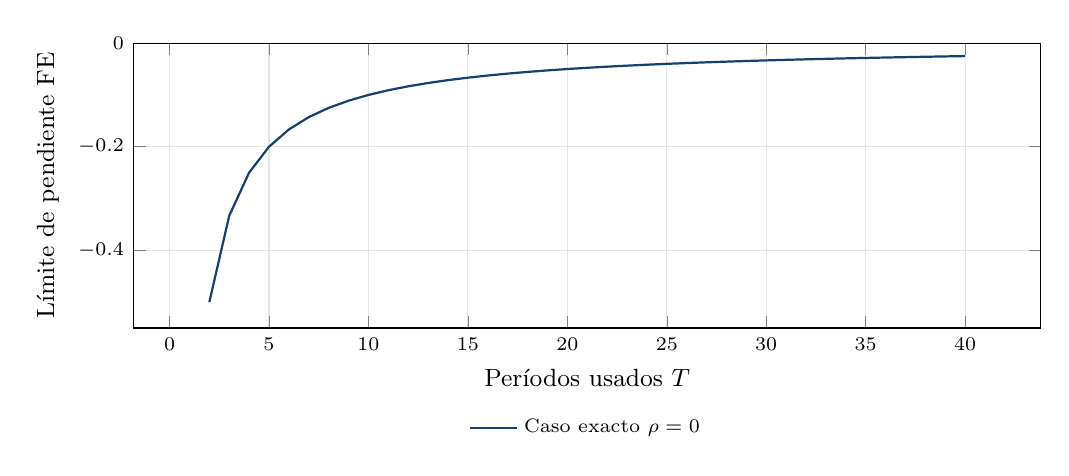
\begin{tikzpicture}
\begin{axis}[panelaxis,xlabel={Períodos usados $T$},ylabel={Límite de pendiente FE},ymin=-.55,ymax=0]
\addplot[azul,thick,no marks] coordinates {(2,-0.5) (3,-0.333333333) (4,-0.25) (5,-0.2) (6,-0.166666667) (7,-0.142857143) (8,-0.125) (9,-0.111111111) (10,-0.1) (11,-0.0909090909) (12,-0.0833333333) (13,-0.0769230769) (14,-0.0714285714) (15,-0.0666666667) (16,-0.0625) (17,-0.0588235294) (18,-0.0555555556) (19,-0.0526315789) (20,-0.05) (21,-0.0476190476) (22,-0.0454545455) (23,-0.0434782609) (24,-0.0416666667) (25,-0.04) (26,-0.0384615385) (27,-0.037037037) (28,-0.0357142857) (29,-0.0344827586) (30,-0.0333333333) (31,-0.0322580645) (32,-0.03125) (33,-0.0303030303) (34,-0.0294117647) (35,-0.0285714286) (36,-0.0277777778) (37,-0.027027027) (38,-0.0263157895) (39,-0.0256410256) (40,-0.025)};
\addlegendentry{Caso exacto $\rho=0$}
\end{axis}
\end{tikzpicture}
\caption{En el caso independiente $y_{it}=\eps_{it}$, la pendiente dinámica FE converge a $-1/T$ con muchas entidades. El valor verdadero es cero.}\label{fig:panel-13}
\end{figure}
% FIN PANELFIG
\section{Sesgo de Nickell y su orden}
Para un AR(1) estacionario con interceptos individuales y supuestos clásicos, una expansión de gran $T$ del límite de FE tiene sesgo principal
\[
\widehat\rho_{\rm FE}-\rho
\ \text{del orden de}\ -\frac{1+\rho}{T-1}.
\]
La expresión es una aproximación de primer orden, no una identidad exacta para todo $T$, ni un sustituto del ejemplo anterior.
La condición inicial, los regresores adicionales y el proceso de errores pueden cambiar términos y condiciones.
El punto central es que aumentar $G$ con $T$ fijo no elimina este sesgo.
Si $T\to\infty$, la escala $1/T$ puede hacerse pequeña, pero hay que compararla con la precisión de la inferencia.

\section{Anderson--Hsiao: diferenciar e instrumentar}
Al restar el período anterior:
\[
\Delta y_{it}=\rho\Delta y_{i,t-1}
+\Delta x_{it}\T\beta+\Delta\eps_{it}.
\]
$\Delta y_{i,t-1}$ contiene $\eps_{i,t-1}$; el error contiene $-\eps_{i,t-1}$.
Por eso MCO en diferencias es endógeno.
Si los errores originales no están autocorrelacionados y los antecedentes satisfacen las condiciones adecuadas,
\[
\E[y_{i,t-2}\Delta\eps_{it}]=0.
\]
El nivel $y_{i,t-2}$ puede instrumentar $\Delta y_{i,t-1}$.
También una diferencia rezagada puede ser válida, con otras condiciones y relevancia. La selección no se hace solo por disponibilidad: se deduce cada momento.

\section{Arellano--Bond: desplegar la matriz triangular}
Si $\E(y_{is}\eps_{it})=0$ para $s\le t-1$ bajo las restricciones dinámicas pertinentes, entonces
$\E[y_{is}(\eps_{it}-\eps_{i,t-1})]=0$ para $s\le t-2$.
Con observaciones $y_{i0},y_{i1},y_{i2},y_{i3},y_{i4}$, las ecuaciones diferenciadas útiles son $t=2,3,4$:
\[
\begin{pmatrix}\Delta y_{i2}\\\Delta y_{i3}\\\Delta y_{i4}\end{pmatrix}
=\rho\begin{pmatrix}\Delta y_{i1}\\\Delta y_{i2}\\\Delta y_{i3}\end{pmatrix}
+\begin{pmatrix}\Delta\eps_{i2}\\\Delta\eps_{i3}\\\Delta\eps_{i4}\end{pmatrix}
\]
si omitimos $x$ para mostrar la estructura.
Una matriz de instrumentos no colapsada es
\[
Z_i=\begin{pmatrix}
y_{i0}&0&0&0&0&0\\
0&y_{i0}&y_{i1}&0&0&0\\
0&0&0&y_{i0}&y_{i1}&y_{i2}
\end{pmatrix}.
\]
Cada columna representa un momento en una ecuación específica.
No se debe tratar una columna con ceros de diseño como una variable observada común en todas las fechas.
El vector $Z_i\T\Delta\eps_i$ tiene seis momentos.

\section{Covarianza de diferencias y GMM de una etapa}
Con errores originales esféricos,
\[
\Var(\Delta\eps_i)=\sigma^2
\begin{pmatrix}
2&-1&0\\-1&2&-1\\0&-1&2
\end{pmatrix}
=\sigma^2H.
\]
Un peso de una etapa puede basarse en
$(\sum_iZ_i\T HZ_i)^{-1}$, sin el factor $\sigma^2$ que se cancela en la estimación.
El estimador GMM utiliza los momentos definidos en el capítulo anterior.
Dos etapas reemplazan la covarianza de trabajo por un estimador basado en residuos por entidad:
$\widehat S=G^{-1}\sum_iZ_i\T\widehat u_i\widehat u_i\T Z_i$.
La varianza reportada debe reconocer el uso de un peso estimado; la corrección de Windmeijer atiende un problema específico de muestra finita en GMM de dos etapas.

\section{AR(1) esperado y AR(2) que amenaza instrumentos}
Aunque $\eps_{it}$ sea serialmente independiente,
$\Delta\eps_{it}$ tiene covarianza $-\sigma^2$ con $\Delta\eps_{i,t-1}$.
Por ello rechazar ausencia de AR(1) en residuos diferenciados puede ser esperado bajo el modelo válido.
En cambio,
\[
\Cov(\Delta\eps_{it},\Delta\eps_{i,t-2})=0
\]
bajo independencia temporal original.
Una señal AR(2) en diferencias puede indicar que momentos basados en ciertos niveles rezagados no son válidos.
Las pruebas usan residuos estimados y correcciones por estimación; no son simples correlaciones muestrales comparadas con una normal sin ajuste.

\section{System GMM: momentos nuevos, supuestos nuevos}
Si el proceso satisface restricciones adicionales de condición inicial y de medias, puede cumplirse
\[
\E[\Delta y_{i,t-1}(a_i+\eps_{it})]=0.
\]
Esto permite usar diferencias rezagadas como instrumentos en ecuaciones de niveles, junto con los instrumentos de niveles para ecuaciones diferenciadas.
La condición no se deduce automáticamente de ausencia de autocorrelación: exige, entre otras cosas, una relación adecuada entre diferencias y heterogeneidad individual.
Una condición de estacionariedad de la media del proceso es una justificación frecuente, pero debe evaluarse en el contexto.

El sistema apila ambos bloques:
\[
y_i^{\rm sys}=\begin{pmatrix}\Delta y_i\\y_i\end{pmatrix},
\quad
X_i^{\rm sys}=\begin{pmatrix}\Delta X_i\\X_i\end{pmatrix},
\quad
Z_i^{\rm sys}=\begin{pmatrix}Z_i^\Delta&0\\0&Z_i^L\end{pmatrix}.
\]
Los errores de bloques pueden estar correlacionados; GMM robusto estima su covarianza conjunta por entidad. Agregar ecuaciones no crea validez instrumental.

\section{Proliferación de instrumentos y persistencia}
La matriz triangular no colapsada genera un número de momentos que crece aproximadamente como $T^2$.
Muchos instrumentos pueden ajustar demasiado los regresores endógenos, aumentar sesgo de muestra finita y deteriorar la prueba J.
Se pueden limitar ventanas de rezagos o colapsar momentos, pero cambia la información utilizada y debe documentarse.

Si $\rho$ está cerca de uno, un nivel pasado puede predecir débilmente una diferencia:
en un proceso muy persistente, niveles similares se cancelan al diferenciar.
System GMM intenta aportar otra información bajo supuestos adicionales; no garantiza identificación fuerte en todos los casos.



% PANELFIG 14
\begin{figure}[htbp]\centering
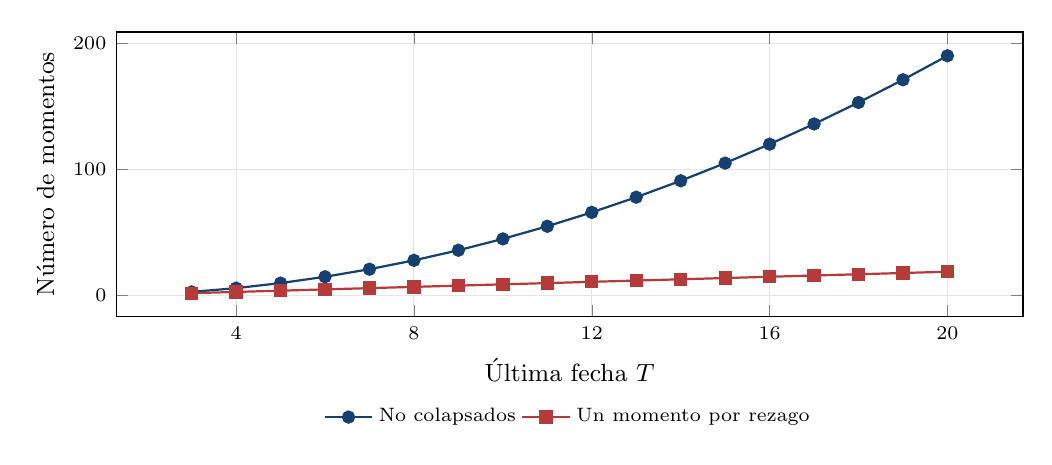
\begin{tikzpicture}
\begin{axis}[panelaxis,xlabel={Última fecha $T$},ylabel={Número de momentos},xtick={4,8,12,16,20}]
\addplot[azul,thick,mark=*] coordinates {(3,3) (4,6) (5,10) (6,15) (7,21) (8,28) (9,36) (10,45) (11,55) (12,66) (13,78) (14,91) (15,105) (16,120) (17,136) (18,153) (19,171) (20,190)};
\addlegendentry{No colapsados}
\addplot[rojo,thick,mark=square*] coordinates {(3,2) (4,3) (5,4) (6,5) (7,6) (8,7) (9,8) (10,9) (11,10) (12,11) (13,12) (14,13) (15,14) (16,15) (17,16) (18,17) (19,18) (20,19)};
\addlegendentry{Un momento por rezago}
\end{axis}
\end{tikzpicture}
\caption{Conteo ilustrativo de momentos para ecuaciones $t=2,\ldots,T$, con antecedentes desde $y_0$. Colapsar o limitar rezagos cambia la dimensión y la información del sistema.}\label{fig:panel-14}
\end{figure}
% FIN PANELFIG
\section{Corregir sesgo, usar panel largo o cambiar el estimando}
Con $T$ moderado o grande, existen aproximaciones analíticas y jackknife para corregir sesgo FE dinámico.
Un split-panel jackknife compara la estimación completa con estimaciones en mitades temporales.
Si el sesgo principal es $b/T$, cada mitad tiene aproximadamente $2b/T$;
$2\widehat\rho_{\rm completo}-(\widehat\rho_{\rm mitad1}+\widehat\rho_{\rm mitad2})/2$ cancela ese término.
La validez requiere estabilidad del proceso y una expansión apropiada; puede aumentar varianza y no corrige automáticamente cambios estructurales.

\section{Varianza del efecto de largo plazo por método delta}
Sea $h(\rho,\beta)=\beta/(1-\rho)$.
Su gradiente es
\[
\nabla h=\begin{pmatrix}\beta/(1-\rho)^2\\1/(1-\rho)\end{pmatrix}.
\]
Para una covarianza estimada conjunta de $(\widehat\rho,\widehat\beta)$,
\[
\Var(\widehat h)\approx
\frac{\beta^2V_{\rho\rho}}{(1-\rho)^4}
+\frac{V_{\beta\beta}}{(1-\rho)^2}
+\frac{2\beta V_{\rho\beta}}{(1-\rho)^3}.
\]
Es una aproximación local. Cerca de $\rho=1$, el gradiente explota y la aproximación normal puede ser deficiente. El intervalo debe reflejar la debilidad de determinar el denominador, no solo la precisión de $\widehat\beta$.

\section{Curiosidad: una condición inicial puede cambiar toda la estrategia}
En RE dinámico, $y_{i0}$ suele contener información sobre $a_i$.
Tratarlo como un regresor exógeno independiente del efecto aleatorio puede ser incorrecto.
En GMM, los primeros rezagos disponibles y su validez dependen de cómo se originó la trayectoria.
La primera fila de una base no es necesariamente el inicio económico del proceso; puede ser solo el inicio de observación.



% MODULO 10_causalidad.tex
\parte{X. Panel y causalidad: de la comparación a las condiciones}
\section{Resultados potenciales y el efecto que buscamos}
Para tratamiento binario $D_{it}$, sean $Y_{it}(0)$ y $Y_{it}(1)$ los resultados potenciales sin y con tratamiento. Observamos
$Y_{it}=(1-D_{it})Y_{it}(0)+D_{it}Y_{it}(1)$.
Nunca observamos simultáneamente ambos resultados de la misma entidad en la misma fecha.
Un efecto medio sobre tratados es
$\E[Y_{it}(1)-Y_{it}(0)\mid D_{it}=1]$.
Una regresión describe asociaciones; para interpretar un coeficiente como ese efecto se requieren restricciones sobre la trayectoria contrafactual.

Los efectos fijos eliminan diferencias permanentes. No eliminan automáticamente tendencias específicas, cambios de composición, anticipación o tratamientos decididos por choques temporales no observados.

\section{DID de dos grupos y dos períodos}
Sea $A$ el grupo tratado y $B$ el control, con fechas $0$ y $1$.
La diferencia en diferencias es
\[
\widehat\tau
=(\bar Y_{A1}-\bar Y_{A0})-(\bar Y_{B1}-\bar Y_{B0}).
\]
Con ausencia de tratamiento en fecha $0$ y ausencia de anticipación, identifica el efecto medio sobre $A$ en fecha $1$ si
\[
\E[Y_{A1}(0)-Y_{A0}(0)]
=\E[Y_{B1}(0)-Y_{B0}(0)].
\]
Esta es la restricción de tendencias paralelas. No exige niveles iguales.

\begin{deduccion}
Sumamos y restamos $\E Y_{A1}(0)$ en el primer cambio. El DID poblacional es
\[
\E[Y_{A1}(1)-Y_{A1}(0)]
+\{\E[Y_{A1}(0)-Y_{A0}(0)]
-\E[Y_{B1}(0)-Y_{B0}(0)]\}.
\]
El término entre llaves es cero por tendencias paralelas.
\end{deduccion}

\begin{resuelto}{Cambio común y efecto adicional}
Los promedios sintéticos son
$Y_{A0}=10$, $Y_{A1}=17$, $Y_{B0}=8$, $Y_{B1}=11$.
El cambio tratado es $7$ y el control $3$; DID $=4$.
El contrafactual tratado sería $10+3=13$, así que $17-13=4$.
Si sin tratamiento el grupo $A$ habría aumentado $5$ en lugar de $3$, el efecto verdadero sería $17-15=2$ y DID tendría sesgo $2$.
Los cuatro números observados no permiten verificar ese contrafactual.
\end{resuelto}



% PANELFIG 15
\begin{figure}[htbp]\centering
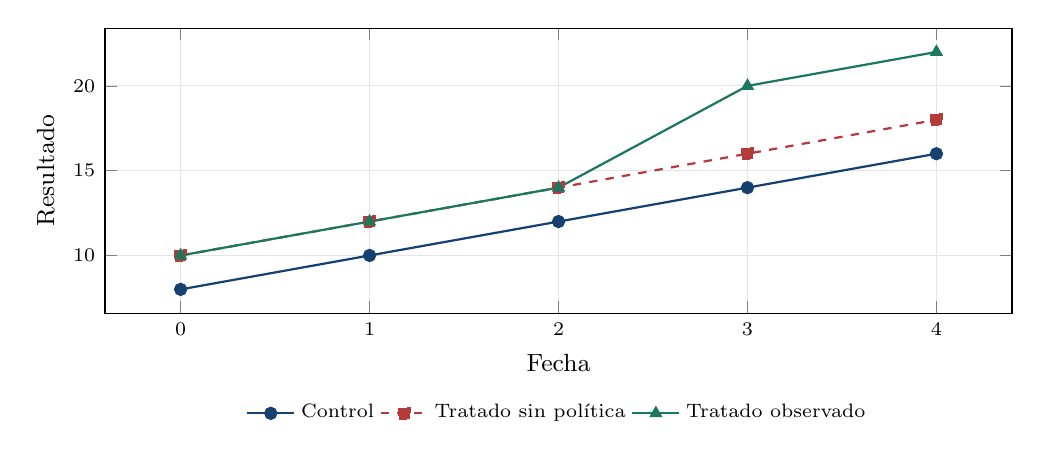
\begin{tikzpicture}
\begin{axis}[panelaxis,xlabel={Fecha},ylabel={Resultado},xtick={0,1,2,3,4}]
\addplot[azul,thick,mark=*] coordinates {(0,8) (1,10) (2,12) (3,14) (4,16)};
\addlegendentry{Control}
\addplot[rojo,thick,dashed,mark=square*] coordinates {(0,10) (1,12) (2,14) (3,16) (4,18)};
\addlegendentry{Tratado sin política}
\addplot[verde,thick,mark=triangle*] coordinates {(0,10) (1,12) (2,14) (3,20) (4,22)};
\addlegendentry{Tratado observado}
\end{axis}
\end{tikzpicture}
\caption{Diseño sintético con tendencias paralelas y adopción en fecha 3. La trayectoria contrafactual del tratado es un supuesto del ejemplo, no un resultado observable.}\label{fig:panel-15}
\end{figure}
% FIN PANELFIG
\section{La regresión de DID y su matriz explícita}
Para las cuatro celdas, orden $A0,A1,B0,B1$, sea $A_j$ el indicador de grupo tratado y $P_j$ el indicador posterior.
\[
Z=\begin{pmatrix}
1&1&0&0\\
1&1&1&1\\
1&0&0&0\\
1&0&1&0
\end{pmatrix},\qquad
b=\begin{pmatrix}c\\a\\\lambda\\\tau\end{pmatrix}.
\]
Las cuatro ecuaciones son
$Y_{A0}=c+a$,
$Y_{A1}=c+a+\lambda+\tau$,
$Y_{B0}=c$,
$Y_{B1}=c+\lambda$.
De ellas $\tau$ es exactamente DID.
Con una observación por celda, el modelo saturado tiene cero grados de libertad residuales: no se obtiene una varianza de error de esa tabla sola.
Con múltiples unidades, la estructura de dependencia determina cómo estimar incertidumbre.

\section{La varianza DID con trayectorias correlacionadas}
Si entidades de grupos diferentes son independientes y existen $G_A,G_B$ trayectorias,
\[
\Var(\widehat\tau)
=\frac{\Var(Y_{i1}-Y_{i0}\mid A)}{G_A}
+\frac{\Var(Y_{i1}-Y_{i0}\mid B)}{G_B}.
\]
Dentro de un grupo,
\[
\Var(Y_{i1}-Y_{i0})
=\Var(Y_{i1})+\Var(Y_{i0})-2\Cov(Y_{i1},Y_{i0}).
\]
Si ambos períodos tienen varianza $9$ y covarianza $6$, la varianza del cambio es $6$, no $18$.
Con $G_A=G_B=10$, la varianza DID es $6/10+6/10=1.2$.
Estos números suponen que la unidad independiente es la entidad. Si el tratamiento se asigna por región, puede ser necesario agrupar por región.

\section{Adopción escalonada y el peligro de un único TWFE}
Supongamos que distintas cohortes adoptan en fechas distintas y el tratamiento permanece activo. Una regresión
$Y_{it}=a_i+\lambda_t+\tau D_{it}+u_{it}$ produce
\[
\widehat\tau=\frac{\sum_{it}D_{it}^{\circ}Y_{it}}
{\sum_{it}(D_{it}^{\circ})^2},
\]
donde $D^\circ=M_CD$.
Si el componente sin tratamiento se ajusta al diseño y los efectos son $\tau_{it}$,
\[
\widehat\tau\ \text{combina}\ 
\sum_{D_{it}=1}w_{it}\tau_{it},\qquad
w_{it}=\frac{D_{it}^{\circ}}{\sum_{js}(D_{js}^{\circ})^2}.
\]
Los pesos de celdas tratadas suman uno porque
$D\T M_CD=(D^\circ)\T D^\circ$.
Pero algunos pueden ser negativos; el coeficiente no es necesariamente un promedio convexo de efectos tratados.

\begin{resuelto}{Un peso negativo calculado sin abreviar}
Tres grupos $A,B,C$ y tres fechas tienen
\[
D=\begin{pmatrix}0&1&1\\0&0&1\\0&0&0\end{pmatrix}.
\]
Las medias de filas son $(2/3,1/3,0)$; las de columnas $(0,1/3,2/3)$; la global $1/3$.
\[
D^\circ=\begin{pmatrix}
-1/3&1/3&0\\
0&-1/3&1/3\\
1/3&0&-1/3
\end{pmatrix}.
\]
El peso de $A$ en la tercera fecha es cero, no negativo.
Para mostrar el problema, usemos cuatro fechas:
\[
D=\begin{pmatrix}0&1&1&1\\0&0&0&1\\0&0&0&0\end{pmatrix}.
\]
Las medias individuales son $3/4,1/4,0$; las temporales $0,1/3,1/3,2/3$; la global $1/3$.
En la celda $A4$, $D^\circ_{A4}=1-3/4-2/3+1/3=-1/12$.
La suma de cuadrados transformada es $5/6$.
Los pesos tratados son
$w_{A2}=3/10$, $w_{A3}=3/10$, $w_{A4}=-1/10$, $w_{B4}=1/2$.
Suman $1$.
Con efectos $2,2,20,2$, el coeficiente es
$(3/10)2+(3/10)2-(1/10)20+(1/2)2=1/5$,
aunque todos los efectos sean positivos y su promedio simple sea $6.5$.
\end{resuelto}



% PANELFIG 16
\begin{figure}[htbp]\centering
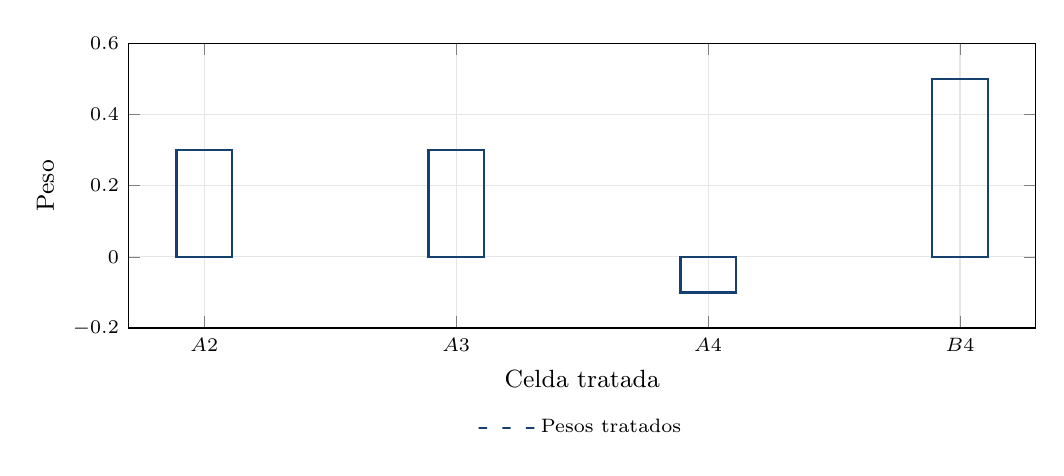
\begin{tikzpicture}
\begin{axis}[panelaxis,xlabel={Celda tratada},ylabel={Peso},xtick={1,2,3,4},xticklabels={$A2$,$A3$,$A4$,$B4$},ymin=-0.2,ymax=0.6]
\addplot[azul,thick,ybar,bar width=20pt] coordinates {(1,0.3) (2,0.3) (3,-0.1) (4,0.5)};
\addlegendentry{Pesos tratados}
\end{axis}
\end{tikzpicture}
\caption{Pesos exactos del ejemplo escalonado de cuatro fechas. El peso negativo de $A4$ permite que un efecto grande positivo reduzca el coeficiente TWFE.}\label{fig:panel-16}
\end{figure}
% FIN PANELFIG
\section{Efectos grupo--tiempo como objetos separados}
Sea $G_i=g$ la fecha de primera adopción, con $G_i=\infty$ para nunca tratados.
Definimos
\[
ATT(g,t)=\E[Y_{it}(1)-Y_{it}(0)\mid G_i=g],\qquad t\ge g.
\]
Bajo ausencia de anticipación y tendencias paralelas pertinentes con un grupo de control $C$ aún no tratado o nunca tratado,
\[
ATT(g,t)=
\E[Y_{it}-Y_{i,g-1}\mid G_i=g]
-\E[Y_{it}-Y_{i,g-1}\mid i\in C].
\]
Cada control debe permanecer sin tratamiento durante el contraste y cumplir la restricción contrafactual. Si se requiere condicionamiento en covariables, la comparación de medias no ajustada puede ser insuficiente.

Se agregan los $ATT(g,t)$ con pesos no negativos elegidos según la pregunta: por cohorte, duración o calendario. El conjunto de cohortes que contribuye puede cambiar con la duración, de modo que un perfil dinámico puede cambiar por composición aun sin cambio de efectos dentro de cohortes.



% PANELFIG 17
\begin{figure}[htbp]\centering
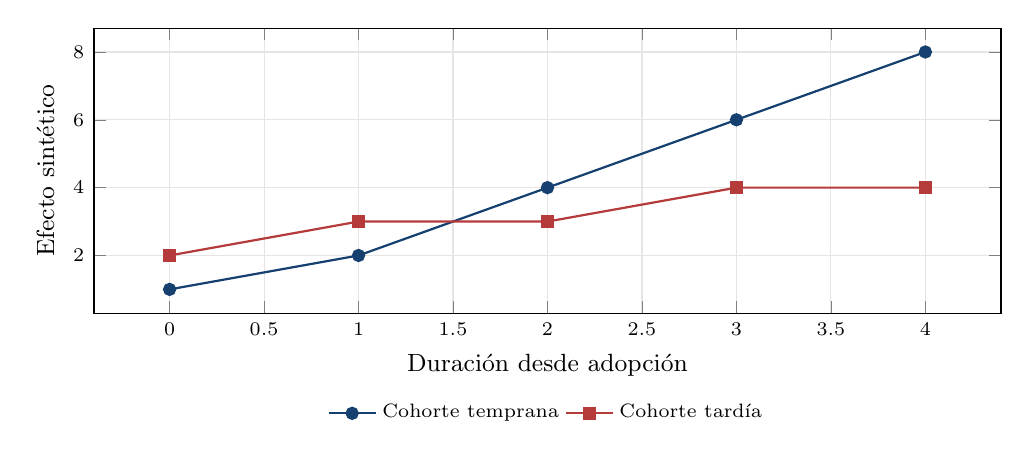
\begin{tikzpicture}
\begin{axis}[panelaxis,xlabel={Duración desde adopción},ylabel={Efecto sintético}]
\addplot[azul,thick,mark=*] coordinates {(0,1) (1,2) (2,4) (3,6) (4,8)};
\addlegendentry{Cohorte temprana}
\addplot[rojo,thick,mark=square*] coordinates {(0,2) (1,3) (2,3) (3,4) (4,4)};
\addlegendentry{Cohorte tardía}
\end{axis}
\end{tikzpicture}
\caption{Dos perfiles de efectos heterogéneos. Su agregación exige declarar los pesos y las cohortes disponibles en cada duración; no son estimaciones de datos reales.}\label{fig:panel-17}
\end{figure}
% FIN PANELFIG
\section{Event study: qué representa cada indicador}
Para duración relativa $\ell=t-G_i$, un indicador es
$D_{it}^\ell=\ind\{t-G_i=\ell\}$.
Se omite una duración base, frecuentemente $-1$.
Un event study TWFE con muchos leads y lags puede mezclar efectos de cohortes y otras duraciones cuando hay heterogeneidad.
Una formulación por interacciones cohorte--duración estima objetos separados y después los agrega con pesos explícitos.

Un coeficiente previo distinto de cero puede reflejar tendencias no paralelas, anticipación o contaminación de la especificación. Un coeficiente previo no significativo no demuestra tendencias paralelas: puede tener poca potencia. La identificación exige un argumento de diseño, no solo un gráfico de intervalos que crucen cero.

\section{Panel verdadero y cortes repetidos en DID}
En panel podemos calcular $Y_{it}-Y_{i0}$ para la misma entidad. En cortes repetidos calculamos diferencias de medias de muestras diferentes.
DID puede construirse en ambos, pero requiere condiciones sobre composición estable o ajustes adecuados.
La varianza de un cambio individual incluye covarianza temporal de la misma persona; una diferencia de medias de muestras independientes no la incluye.
Un identificador de cluster en una regresión pooled no demuestra que las mismas entidades fueron seguidas.

\section{Pesos de tratamiento y estimación doblemente robusta}
Para una comparación de cohortes, sea $p(X)$ la probabilidad de pertenecer a la cohorte tratada entre tratados y controles elegibles; sea $m_0(X)=\E(\Delta Y\mid C,X)$.
Un contraste ponderado construye un cambio contrafactual con controles de pesos proporcionales a $p(X)/(1-p(X))$.
Una representación aumentada resta $m_0(X)$ tanto en tratados como controles ponderados. Bajo las condiciones causales y de solapamiento, esa forma puede permanecer consistente si el modelo de probabilidad o el de regresión de control es correcto, según la formulación precisa.
La doble robustez no significa inmunidad a tendencias paralelas falsas ni a falta de controles comparables.

\section{Curiosidad: FE de tiempo absorbe una política nacional uniforme}
Si todos reciben $D_{it}=D_t$ en la misma fecha, la columna de tratamiento está en el espacio de dummies temporales y $M_CD=0$.
La pendiente no se identifica con un panel de dos vías únicamente.
Se necesita variación adicional, un grupo de comparación u otro diseño.
Tener muchas personas antes y después no crea una comparación contemporánea inexistente.



% MODULO 11_no_lineal_datos.tex
\parte{XI. Datos incompletos, modelos no lineales y estimandos}
\section{Observación, selección y pérdida de seguimiento}
Sea $R_{it}=1$ si observamos la fila y $0$ si falta. El conjunto disponible depende de $R$.
La exogeneidad para datos completos
$\E(\eps_{it}\mid X_i,a_i)=0$
no garantiza
$\E(\eps_{it}\mid X_i,a_i,R_i)=0$.
Si abandonar la encuesta depende de un choque de ingreso, la muestra observada puede seleccionar errores.

Si la probabilidad de observación $\pi_{it}$ es positiva y la selección es ignorable condicional en información apropiada, un peso $R_{it}/\pi_{it}$ puede recuperar ciertos momentos:
\[
\E\left[\frac{R_{it}}{\pi_{it}}h_{it}\,\middle|\,\text{información}\right]
=\E[h_{it}\mid\text{información}]
\]
cuando la independencia condicional y la definición de $\pi_{it}$ justifican pasar $h_{it}$ a través de la esperanza.
Sin positividad, pesos enormes o selección por variables no observadas, no hay recuperación automática.
El modelo de observación es otro componente que debe estimarse y evaluar.

\section{Within ponderado y el orden correcto}
Para pesos positivos $w_{it}$, sea $W=\diag(w_{it})$.
El promedio individual ponderado es
\[
\bar y_{i,w}=\frac{\sum_tw_{it}y_{it}}{\sum_tw_{it}}.
\]
Al minimizar $\sum_{it}w_{it}(y_{it}-a_i-x_{it}\T\beta)^2$,
la derivada en $a_i$ da
$a_i(\beta)=\bar y_{i,w}-\bar x_{i,w}\T\beta$.
Sustituyendo se obtiene MCO ponderado sobre desviaciones respecto de medias ponderadas.
El proyector euclídeo del diseño blanqueado $W^{1/2}D$ es
\[
P_{W^{1/2}D}=W^{1/2}D(D\T WD)^{-1}D\T W^{1/2}.
\]
La transformación en escala original no es simétrica:
$I-D(D\T WD)^{-1}D\T W$.
Confundir ambos operadores produce medias incorrectas.

\section{Logaritmos y la interpretación de un cambio}
Si $y=\log w$ y la pendiente de $x$ es $\beta$, un cambio de una unidad en $x$ cambia la predicción del logaritmo en $\beta$.
Para el valor geométrico exponenciado, la razón es $e^\beta$ y el porcentaje exacto $100(e^\beta-1)$.
$100\beta$ es una aproximación para $\beta$ pequeño.
Pero
$\E(w\mid X)\ne\exp[\E(\log w\mid X)]$ en general.
Si $\log w=m(X)+u$, $u\mid X\sim N(0,\sigma^2)$,
\[
\E(w\mid X)=\exp[m(X)+\sigma^2/2].
\]
La corrección cambia con heterocedasticidad.
El logaritmo exige $w>0$; eliminar ceros puede cambiar la población estudiada.

\section{Modelo lineal de probabilidad}
Para $Y_{it}\in\{0,1\}$, $\E(Y_{it}\mid X,a)=p_{it}$.
Una especificación lineal $p_{it}=a_i+x_{it}\T\beta$ permite FE lineal, pero puede producir predicciones fuera de $[0,1]$.
La varianza condicional es $p_{it}(1-p_{it})$, de modo que es heterocedástica por construcción.
La pendiente representa un cambio de probabilidad en la aproximación lineal. No se interpreta como un log-odds.

\section{Logit con efectos fijos y parámetros incidentales}
El logit especifica
\[
p_{it}=\frac{\exp(a_i+x_{it}\T\beta)}{1+\exp(a_i+x_{it}\T\beta)}.
\]
La log-verosimilitud condicional en regresores y efectos es
\[
\ell(a,\beta)=\sum_i\sum_t
[y_{it}(a_i+x_{it}\T\beta)-\log(1+e^{a_i+x_{it}\T\beta})].
\]
La derivada en $\beta$ es $\sum_{it}x_{it}(y_{it}-p_{it})$ y el Hessiano es
$-\sum_{it}p_{it}(1-p_{it})x_{it}x_{it}\T$.
No hay una transformación por medias que elimine $a_i$ de la función logística.
Estimar muchos interceptos con $T$ pequeño puede sesgar pendientes en la máxima verosimilitud no condicionada.

\section{Logit condicional: eliminar mediante un estadístico suficiente}
Bajo independencia temporal condicional de los resultados binarios y la especificación logit, sea $S_i=\sum_ty_{it}$.
La probabilidad de una trayectoria $d=(d_1,\ldots,d_T)$, condicionando en $S_i=s$, es
\[
\Prob(Y_i=d\mid S_i=s,X_i)
=\frac{\exp(\sum_td_tx_{it}\T\beta)}
{\sum_{c:\sum_tc_t=s}\exp(\sum_tc_tx_{it}\T\beta)}.
\]
El factor $\exp(a_i s)$ se cancela entre numerador y denominador.
Por eso la verosimilitud condicional no incluye $a_i$.
Entidades con todos ceros o todos unos tienen $s=0$ o $s=T$; solo hay una trayectoria posible y no aportan información condicional a la pendiente.

Para $T=2$, $S_i=1$, existen $(1,0)$ y $(0,1)$:
\[
\Prob[(0,1)\mid S_i=1,X_i]
=\frac{\exp(x_{i2}\T\beta)}
{\exp(x_{i1}\T\beta)+\exp(x_{i2}\T\beta)}
=\frac1{1+\exp[-(x_{i2}-x_{i1})\T\beta]}.
\]
La comparación es entre covariables de fechas de la misma entidad.
Una dependencia temporal más general puede invalidar esa verosimilitud condicional, aunque una covarianza robusta no repara su media o estructura probabilística incorrecta.



% PANELFIG 18
\begin{figure}[htbp]\centering
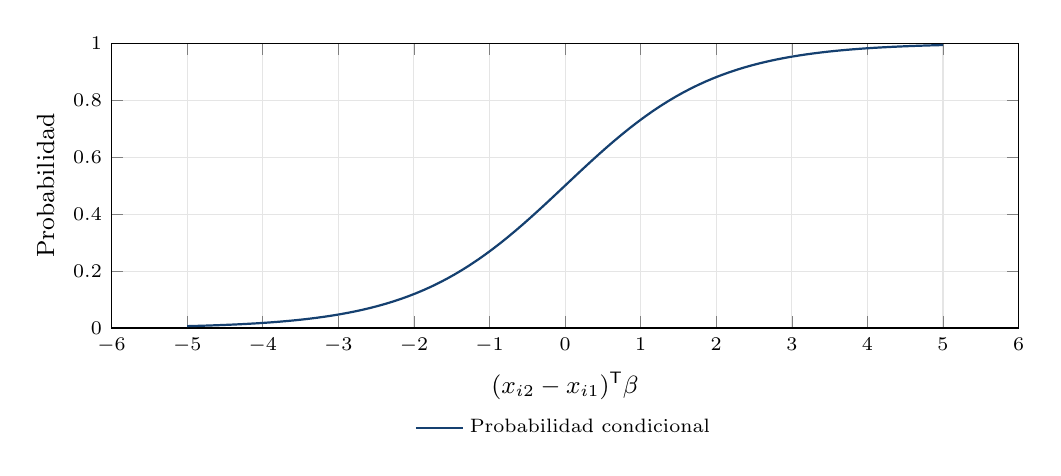
\begin{tikzpicture}
\begin{axis}[panelaxis,xlabel={$(x_{i2}-x_{i1})^{\mathsf T}\beta$},ylabel={Probabilidad},ymin=0,ymax=1]
\addplot[azul,thick,no marks] coordinates {(-5,0.00669285092) (-4.8989899,0.00739895605) (-4.7979798,0.00817894286) (-4.6969697,0.00904040581) (-4.5959596,0.00999168994) (-4.49494949,0.0110419583) (-4.39393939,0.0122012643) (-4.29292929,0.0134806277) (-4.19191919,0.0148921164) (-4.09090909,0.0164489307) (-3.98989899,0.0181654925) (-3.88888889,0.0200575365) (-3.78787879,0.022142204) (-3.68686869,0.0244381366) (-3.58585859,0.0269655704) (-3.48484848,0.0297464254) (-3.38383838,0.0328043909) (-3.28282828,0.0361650012) (-3.18181818,0.0398556989) (-3.08080808,0.0439058811) (-2.97979798,0.0483469227) (-2.87878788,0.0532121708) (-2.77777778,0.0585369029) (-2.67676768,0.064358241) (-2.57575758,0.070715012) (-2.47474747,0.0776475461) (-2.37373737,0.0851974011) (-2.27272727,0.0934070047) (-2.17171717,0.102319204) (-2.07070707,0.11197671) (-1.96969697,0.122421439) (-1.86868687,0.133693736) (-1.76767677,0.145831484) (-1.66666667,0.158869105) (-1.56565657,0.172836464) (-1.46464646,0.187757689) (-1.36363636,0.203649934) (-1.26262626,0.220522127) (-1.16161616,0.238373744) (-1.06060606,0.257193653) (-0.95959596,0.276959098) (-0.858585859,0.297634885) (-0.757575758,0.319172827) (-0.656565657,0.341511511) (-0.555555556,0.364576441) (-0.454545455,0.388280589) (-0.353535354,0.41252537) (-0.252525253,0.437202046) (-0.151515152,0.462193511) (-0.0505050505,0.487376421) (0.0505050505,0.512623579) (0.151515152,0.537806489) (0.252525253,0.562797954) (0.353535354,0.58747463) (0.454545455,0.611719411) (0.555555556,0.635423559) (0.656565657,0.658488489) (0.757575758,0.680827173) (0.858585859,0.702365115) (0.95959596,0.723040902) (1.06060606,0.742806347) (1.16161616,0.761626256) (1.26262626,0.779477873) (1.36363636,0.796350066) (1.46464646,0.812242311) (1.56565657,0.827163536) (1.66666667,0.841130895) (1.76767677,0.854168516) (1.86868687,0.866306264) (1.96969697,0.877578561) (2.07070707,0.88802329) (2.17171717,0.897680796) (2.27272727,0.906592995) (2.37373737,0.914802599) (2.47474747,0.922352454) (2.57575758,0.929284988) (2.67676768,0.935641759) (2.77777778,0.941463097) (2.87878788,0.946787829) (2.97979798,0.951653077) (3.08080808,0.956094119) (3.18181818,0.960144301) (3.28282828,0.963834999) (3.38383838,0.967195609) (3.48484848,0.970253575) (3.58585859,0.97303443) (3.68686869,0.975561863) (3.78787879,0.977857796) (3.88888889,0.979942463) (3.98989899,0.981834507) (4.09090909,0.983551069) (4.19191919,0.985107884) (4.29292929,0.986519372) (4.39393939,0.987798736) (4.49494949,0.988958042) (4.5959596,0.99000831) (4.6969697,0.990959594) (4.7979798,0.991821057) (4.8989899,0.992601044) (5,0.993307149)};
\addlegendentry{Probabilidad condicional}
\end{axis}
\end{tikzpicture}
\caption{Con dos fechas y un único éxito, logit condicional compara las características de las dos fechas. Un nivel individual común se cancela.}\label{fig:panel-18}
\end{figure}
% FIN PANELFIG
\section{Poisson FE: trabajar con la media}
Para un conteo no negativo,
$\mu_{it}=\exp(a_i+x_{it}\T\beta)$.
La función objetivo Poisson, omitiendo constantes,
\[
\ell=\sum_{it}[y_{it}(a_i+x_{it}\T\beta)-e^{a_i+x_{it}\T\beta}]
\]
tiene score $\sum_{it}x_{it}(y_{it}-\mu_{it})$.
La derivada en $a_i$ exige $\sum_t\mu_{it}=\sum_ty_{it}$.
Si el total $S_i>0$,
\[
e^{a_i(\beta)}=\frac{S_i}{\sum_t e^{x_{it}\T\beta}}.
\]
Sustituirlo perfila los interceptos.
Con media condicional correctamente especificada y condiciones de regularidad apropiadas, Poisson pseudo-ML puede ser consistente sin exigir que la varianza sea exactamente la media, usando covarianza robusta adecuada.
La interpretación multiplicativa es $e^{\beta_k}$ por unidad de $x_k$.
Una entidad con total cero requiere una solución límite para su intercepto y no aporta la misma información a la pendiente perfilada.

\section{Heterogeneidad de pendientes y qué promedio aprende FE}
Suponga $y_{it}=a_i+x_{it}\beta_i+\eps_{it}$ con un regresor.
Bajo ortogonalidad del error,
\[
\widehat\beta_{\rm FE}
=\frac{\sum_i q_i\beta_i}{\sum_iq_i}
+\frac{\sum_i\sum_t\widetilde x_{it}\eps_{it}}{\sum_iq_i},
\qquad q_i=\sum_t\widetilde x_{it}^2.
\]
FE pondera las pendientes por variación within, no necesariamente por un individuo--un voto.
Si individuos con más cambio en $x$ tienen efectos mayores, esa media difiere de $G^{-1}\sum_i\beta_i$.
Con varios regresores aparecen matrices de ponderación, y la interpretación de cada coeficiente como promedio simple se vuelve más delicada.

\section{Error de medición: una deducción de atenuación within}
Sea $x^{\rm obs}=x+\eta$, con $\eta$ de media cero y ortogonal a $x,\eps$, y un modelo verdadero $y=a+\beta x+\eps$.
En una población de muchas entidades con momentos estables,
\[
\beta_{\rm FE}^{*}
=\beta\,
\frac{\E(x_i\T M_ix_i)}
{\E(x_i\T M_ix_i)+\E(\eta_i\T M_i\eta_i)}.
\]
Se deduce expandiendo el producto cruzado transformado y usando ortogonalidad.
Si la medición contiene un sesgo permanente $\eta_{it}=b_i$, within lo elimina.
Si contiene ruido temporal independiente, within lo conserva parcialmente.
La estructura temporal del error de medición determina la dirección y magnitud del problema; errores no clásicos pueden producir otros sesgos.

\section{Unidades, escalas e interacciones}
Si $x^*=x/100$, entonces $x\beta=x^*(100\beta)$.
El coeficiente se multiplica por $100$, su varianza por $100^2$ y su estadístico t queda igual.
Si cambiamos un logaritmo natural por logaritmo base 10, se introduce el factor $1/\log 10$.
Una interacción $x_{it}z_i$ puede variar en el tiempo aunque $z_i$ solo no varíe.
Después de within,
$M_i(x_iz_i)=z_iM_ix_i$.
Así FE puede estimar diferencias de pendientes por una característica invariante, aun sin estimar su efecto de nivel separado.

\section{Curiosidad: no existe un único modelo llamado «panel normal»}
«Normal» puede referirse a errores gaussianos, a un modelo clásico de corte transversal o a una distribución multivariada de efectos.
Son afirmaciones diferentes.
Una regresión FE lineal puede tener errores no normales y una teoría asintótica válida.
Un modelo RE normal añade una distribución conjunta específica.
La claridad empieza nombrando el objeto que es normal y la información respecto de la cual se condiciona.



% MODULO 12_dimension.tex
\parte{XII. Dimensiones grandes: estabilidad, proyecciones y predicción}
\section{Por qué no conviene invertir una matriz explícitamente}
La fórmula $(X\T X)^{-1}X\T y$ define MCO, pero una implementación estable resuelve un sistema.
Si $X=QR$, donde las columnas de $Q$ son ortonormales y $R$ es triangular de rango completo, las ecuaciones se reducen a
$R\widehat\beta=Q\T y$.
La sustitución hacia atrás evita formar una inversa.
Además, el número de condición espectral satisface
$\kappa_2(X\T X)=\kappa_2(X)^2$.
Formar productos cruzados puede amplificar pérdida de precisión cuando las columnas son casi dependientes.

Para datos FE, primero se eliminan efectos y luego se aplica QR a $\widetilde X$.
Una variable que era informativa en niveles puede ser casi singular después de within.
La tolerancia de rango debe aplicarse a la escala y al diseño transformado.

\section{SVD y direcciones no identificadas}
La descomposición singular es
$X=U\Sigma V\T$.
Los valores singulares $\sigma_j$ indican cuánto cambia $Xb$ al mover $b$ en la dirección $v_j$.
Si $\sigma_j=0$, existe una combinación de coeficientes que no cambia el ajuste.
La solución de norma mínima es $X^+y$, donde
$X^+=V\Sigma^+U\T$ invierte únicamente valores singulares no nulos.
Una pseudoinversa da una convención numérica; no convierte un coeficiente no identificado en un efecto estimable.

Un valor singular pequeño produce varianza grande en esa dirección:
bajo errores esféricos,
$\Var(v_j\T\widehat\beta)=\sigma^2/\sigma_j^2$.
La colinealidad es una propiedad del diseño, no un defecto que se arregle agregando decimales al reporte.

\section{Un ejemplo de columnas casi iguales}
Sean
\[
X=\begin{pmatrix}1&1\\-1&-1\\0&\delta\end{pmatrix},
\quad
X\T X=\begin{pmatrix}2&2\\2&2+\delta^2\end{pmatrix}.
\]
El determinante es $2\delta^2$ y
\[
(X\T X)^{-1}
=\frac1{2\delta^2}
\begin{pmatrix}2+\delta^2&-2\\-2&2\end{pmatrix}.
\]
La varianza de $\widehat\beta_2$ es $\sigma^2/\delta^2$.
La suma $\beta_1+\beta_2$ puede ser precisa aunque los coeficientes separados no lo sean. El vector de contraste determina qué combinación está identificada con suficiente información.



% PANELFIG 20
\begin{figure}[htbp]\centering
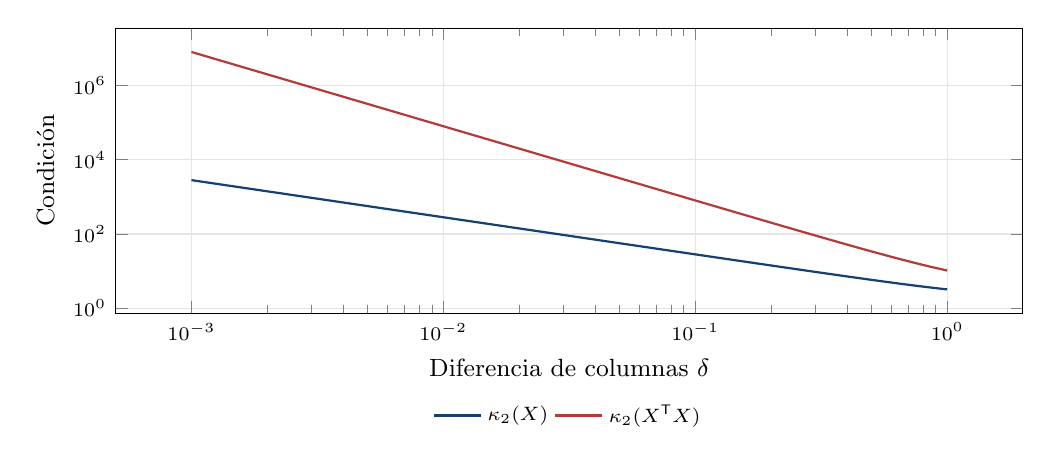
\begin{tikzpicture}
\begin{axis}[panelaxis,xlabel={Diferencia de columnas $\delta$},ylabel={Condición},xmode=log,ymode=log,xtick={0.001,0.01,0.1,1},ytick={1,100,10000,1000000,100000000}]
\addplot[azul,thick,no marks] coordinates {(0.001,2828.42748) (0.00110529514,2558.97945) (0.00122167735,2315.20021) (0.00135031404,2094.64442) (0.00149249555,1895.09974) (0.00164964807,1714.56454) (0.001823348,1551.22791) (0.00201533769,1403.45143) (0.00222754295,1269.75279) (0.0024620924,1148.79087) (0.00272133877,1039.35231) (0.00300788252,940.33936) (0.00332459793,850.758826) (0.00367466194,769.712138) (0.00406158599,696.386329) (0.00448925126,630.045878) (0.0049619476,570.025332) (0.00548441658,515.722633) (0.00606189899,466.593079) (0.0067001875,422.143857) (0.00740568469,381.929103) (0.00818546731,345.545429) (0.00904735724,312.627875) (0.01,282.846248) (0.0110529514,255.901814) (0.0122167735,231.524297) (0.0135031404,209.469169) (0.0149249555,189.515198) (0.0164964807,171.462228) (0.01823348,155.129173) (0.0201533769,140.352198) (0.0222754295,126.983076) (0.024620924,114.887705) (0.0272133877,103.944757) (0.0300788252,94.0444654) (0.0332459793,85.0875209) (0.0367466194,76.984078) (0.0406158599,69.6528522) (0.0448925126,63.020305) (0.049619476,57.0199063) (0.0548441658,51.5914671) (0.0606189899,46.6805355) (0.067001875,42.2378509) (0.0740568469,38.2188495) (0.0818546731,34.5832178) (0.0904735724,31.2944875) (0.1,28.3196708) (0.110529514,25.6289284) (0.122167735,23.1952712) (0.135031404,20.9942891) (0.149249555,19.0039067) (0.164964807,17.2041618) (0.1823348,15.5770056) (0.201533769,14.1061219) (0.222754295,12.776764) (0.24620924,11.5756076) (0.272133877,10.4906179) (0.300788252,9.5109302) (0.332459793,8.62674247) (0.367466194,7.82921957) (0.406158599,7.11040752) (0.448925126,6.46315778) (0.49619476,5.88106111) (0.548441658,5.35839056) (0.606189899,4.89005361) (0.67001875,4.47155377) (0.740568469,4.09896161) (0.818546731,3.76889558) (0.904735724,3.47851231) (1,3.22550493)};
\addlegendentry{$\kappa_2(X)$}
\addplot[rojo,thick,no marks] coordinates {(0.001,8000002) (0.00110529514,6548375.85) (0.00122167735,5360152) (0.00135031404,4387535.26) (0.00149249555,3591403.01) (0.00164964807,2939731.55) (0.001823348,2406308.01) (0.00201533769,1969675.92) (0.00222754295,1612272.15) (0.0024620924,1319720.46) (0.00272133877,1080253.23) (0.00300788252,884238.113) (0.00332459793,723790.579) (0.00367466194,592456.775) (0.00406158599,484953.919) (0.00448925126,396957.808) (0.0049619476,324928.879) (0.00548441658,265969.835) (0.00606189899,217709.101) (0.0067001875,178205.436) (0.00740568469,145869.84) (0.00818546731,119401.644) (0.00904735724,97736.188) (0.01,80002) (0.0110529514,65485.7385) (0.0122167735,53603.5001) (0.0135031404,43877.3327) (0.0149249555,35916.0101) (0.0164964807,29399.2956) (0.01823348,24065.0603) (0.0201533769,19698.7394) (0.0222754295,16124.7017) (0.024620924,13199.1848) (0.0272133877,10804.5126) (0.0300788252,8844.36147) (0.0332459793,7239.88621) (0.0367466194,5926.54826) (0.0406158599,4851.51981) (0.0448925126,3971.55884) (0.049619476,3251.26971) (0.0548441658,2661.67947) (0.0606189899,2179.07239) (0.067001875,1784.03605) (0.0740568469,1460.68046) (0.0818546731,1195.99895) (0.0904735724,979.344951) (0.1,802.003753) (0.110529514,656.841971) (0.122167735,538.020604) (0.135031404,440.760174) (0.149249555,361.148469) (0.164964807,295.983183) (0.1823348,242.643103) (0.201533769,198.982674) (0.222754295,163.245699) (0.24620924,133.994692) (0.272133877,110.053065) (0.300788252,90.4577932) (0.332459793,74.4206856) (0.367466194,61.2966791) (0.406158599,50.557895) (0.448925126,41.7724085) (0.49619476,34.5868798) (0.548441658,28.7123494) (0.606189899,23.9126243) (0.67001875,19.9947932) (0.740568469,16.8014863) (0.818546731,14.2045739) (0.904735724,12.1000479) (1,10.403882)};
\addlegendentry{$\kappa_2(X^{\mathsf T}X)$}
\end{axis}
\end{tikzpicture}
\caption{Las ecuaciones normales cuadran el número de condición. QR y SVD ayudan a preservar precisión, pero no añaden información estadística al diseño.}\label{fig:panel-20}
\end{figure}
% FIN PANELFIG
\section{Absorber dummies sin construir una matriz gigante}
La multiplicación $D\T y$ suma por entidad.
La multiplicación $(D\T D)^{-1}D\T y$ calcula medias.
La multiplicación por $D$ las repite en las filas originales.
Por eso $M_Dy$ requiere acumulaciones por grupo, no almacenar $nG$ entradas.
Para dos vías se alternan operaciones por grupos de entidad y fecha.
El costo de una pasada es proporcional al número de entradas de las variables utilizadas.

Si se usa un método iterativo para resolver el ajuste de efectos, conviene verificar
$\norm{D\T\widehat\eps}$ y $\norm{F\T\widehat\eps}$ con escalas apropiadas.
Una tolerancia pequeña de un paso iterativo no implica por sí sola que los coeficientes estén precisos si el diseño está muy mal condicionado.

\section{Ridge después de within}
Una penalización $\lambda\norm\beta^2$, $\lambda>0$, produce
\[
\widehat\beta_\lambda
=(\widetilde X\T\widetilde X+\lambda I_K)^{-1}\widetilde X\T\widetilde y.
\]
Condicionalmente al diseño y bajo media cero:
\[
\E(\widehat\beta_\lambda)-\beta
=-\lambda(Q+\lambda I)^{-1}\beta,
\]
\[
\Var(\widehat\beta_\lambda)
=\sigma^2(Q+\lambda I)^{-1}Q(Q+\lambda I)^{-1}.
\]
Disminuye variabilidad a cambio de sesgo. En una dirección de autovalor $q_j$ de $Q$, el coeficiente se contrae por $q_j/(q_j+\lambda)$.
La elección de escala de cada columna importa: sin estandarización o una penalización adaptada, cambiar unidades modifica la regularización.



% PANELFIG 19
\begin{figure}[htbp]\centering
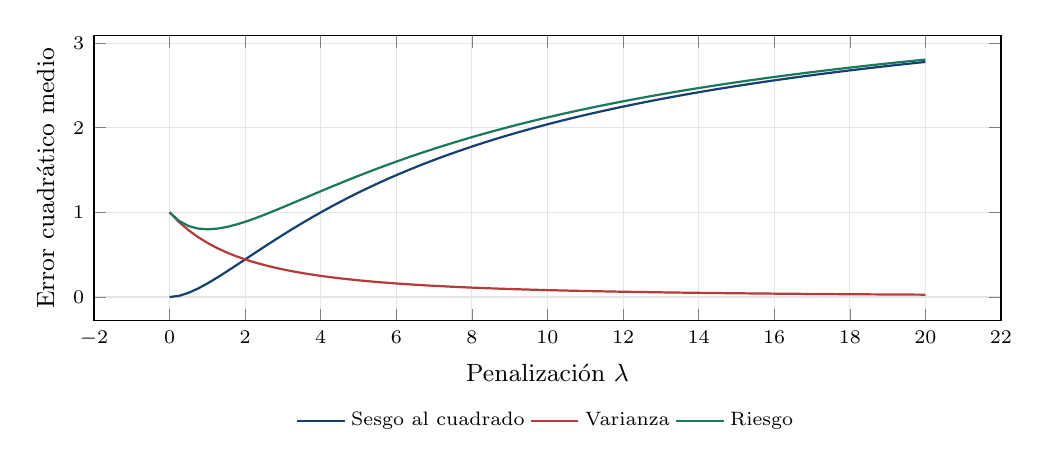
\begin{tikzpicture}
\begin{axis}[panelaxis,xlabel={Penalización $\lambda$},ylabel={Error cuadrático medio}]
\addplot[azul,thick,no marks] coordinates {(0,0) (0.253164557,0.0141723356) (0.506329114,0.0504986744) (0.759493671,0.101856043) (1.01265823,0.163248648) (1.26582278,0.231139053) (1.51898734,0.303004798) (1.7721519,0.377039089) (2.02531646,0.451945484) (2.27848101,0.526795005) (2.53164557,0.600925425) (2.78481013,0.673869459) (3.03797468,0.745303038) (3.29113924,0.815007716) (3.5443038,0.882843115) (3.79746835,0.948726598) (4.05063291,1.01261817) (4.30379747,1.07450922) (4.55696203,1.13441406) (4.81012658,1.19236359) (5.06329114,1.24840049) (5.3164557,1.30257561) (5.56962025,1.35494527) (5.82278481,1.40556914) (6.07594937,1.45450872) (6.32911392,1.50182622) (6.58227848,1.54758362) (6.83544304,1.59184208) (7.08860759,1.6346615) (7.34177215,1.67610013) (7.59493671,1.71621441) (7.84810127,1.75505881) (8.10126582,1.7926857) (8.35443038,1.82914539) (8.60759494,1.86448606) (8.86075949,1.8987538) (9.11392405,1.93199267) (9.36708861,1.96424472) (9.62025316,1.99555009) (9.87341772,2.02594704) (10.1265823,2.05547205) (10.3797468,2.08415989) (10.6329114,2.11204368) (10.8860759,2.13915498) (11.1392405,2.16552388) (11.3924051,2.19117902) (11.6455696,2.21614772) (11.8987342,2.240456) (12.1518987,2.26412869) (12.4050633,2.28718945) (12.6582278,2.30966085) (12.9113924,2.33156442) (13.164557,2.3529207) (13.4177215,2.37374932) (13.6708861,2.39406901) (13.9240506,2.41389767) (14.1772152,2.43325238) (14.4303797,2.4521495) (14.6835443,2.47060465) (14.9367089,2.48863279) (15.1898734,2.50624822) (15.443038,2.52346463) (15.6962025,2.54029513) (15.9493671,2.5567523) (16.2025316,2.57284816) (16.4556962,2.58859426) (16.7088608,2.60400165) (16.9620253,2.61908096) (17.2151899,2.63384237) (17.4683544,2.64829566) (17.721519,2.66245021) (17.9746835,2.67631506) (18.2278481,2.68989887) (18.4810127,2.70320997) (18.7341772,2.71625637) (18.9873418,2.72904578) (19.2405063,2.74158562) (19.4936709,2.75388303) (19.7468354,2.76594487) (20,2.77777778)};
\addlegendentry{Sesgo al cuadrado}
\addplot[rojo,thick,no marks] coordinates {(0,1) (0.253164557,0.884495465) (0.506329114,0.787905567) (0.759493671,0.706315075) (1.01265823,0.636771758) (1.26582278,0.577015533) (1.51898734,0.525292484) (1.7721519,0.480224685) (2.02531646,0.440717463) (2.27848101,0.4058923) (2.53164557,0.375037558) (2.78481013,0.347571842) (3.03797468,0.323016407) (3.29113924,0.300974151) (3.5443038,0.281113463) (3.79746835,0.263155675) (4.05063291,0.246865235) (4.30379747,0.232041939) (4.55696203,0.218514758) (4.81012658,0.206136874) (5.06329114,0.194781686) (5.3164557,0.184339556) (5.56962025,0.174715154) (5.82278481,0.165825274) (6.07594937,0.15759703) (6.32911392,0.149966359) (6.58227848,0.142876766) (6.83544304,0.136278278) (7.08860759,0.130126561) (7.34177215,0.124382175) (7.59493671,0.119009935) (7.84810127,0.113978377) (8.10126582,0.109259292) (8.35443038,0.104827331) (8.60759494,0.100659667) (8.86075949,0.0967356935) (9.11392405,0.0930367764) (9.36708861,0.0895460285) (9.62025316,0.0862481171) (9.87341772,0.0831290958) (10.1265823,0.0801762567) (10.3797468,0.0773780004) (10.6329114,0.0747237222) (10.8860759,0.0722037114) (11.1392405,0.0698090625) (11.3924051,0.0675315963) (11.6455696,0.0653637897) (11.8987342,0.0632987139) (12.1518987,0.0613299791) (12.4050633,0.0594516842) (12.6582278,0.0576583734) (12.9113924,0.0559449962) (13.164557,0.0543068717) (13.4177215,0.0527396566) (13.6708861,0.0512393166) (13.9240506,0.0498021003) (14.1772152,0.0484245156) (14.4303797,0.0471033088) (14.6835443,0.0458354448) (14.9367089,0.0446180903) (15.1898734,0.0434485975) (15.443038,0.04232449) (15.6962025,0.0412434494) (15.9493671,0.0402033034) (16.2025316,0.0392020151) (16.4556962,0.0382376728) (16.7088608,0.0373084809) (16.9620253,0.0364127518) (17.2151899,0.0355488975) (17.4683544,0.0347154236) (17.721519,0.033910922) (17.9746835,0.0331340653) (18.2278481,0.0323836012) (18.4810127,0.0316583475) (18.7341772,0.0309571877) (18.9873418,0.0302790662) (19.2405063,0.0296229845) (19.4936709,0.0289879979) (19.7468354,0.0283732116) (20,0.0277777778)};
\addlegendentry{Varianza}
\addplot[verde,thick,no marks] coordinates {(0,1) (0.253164557,0.8986678) (0.506329114,0.838404242) (0.759493671,0.808171118) (1.01265823,0.800020406) (1.26582278,0.808154586) (1.51898734,0.828297281) (1.7721519,0.857263773) (2.02531646,0.892662948) (2.27848101,0.932687305) (2.53164557,0.975962983) (2.78481013,1.0214413) (3.03797468,1.06831945) (3.29113924,1.11598187) (3.5443038,1.16395658) (3.79746835,1.21188227) (4.05063291,1.25948341) (4.30379747,1.30655116) (4.55696203,1.35292882) (4.81012658,1.39850046) (5.06329114,1.44318217) (5.3164557,1.48691517) (5.56962025,1.52966042) (5.82278481,1.57139441) (6.07594937,1.61210575) (6.32911392,1.65179258) (6.58227848,1.69046038) (6.83544304,1.72812036) (7.08860759,1.76478806) (7.34177215,1.8004823) (7.59493671,1.83522435) (7.84810127,1.86903718) (8.10126582,1.90194499) (8.35443038,1.93397272) (8.60759494,1.96514572) (8.86075949,1.99548949) (9.11392405,2.02502944) (9.36708861,2.05379075) (9.62025316,2.08179821) (9.87341772,2.10907614) (10.1265823,2.13564831) (10.3797468,2.16153789) (10.6329114,2.1867674) (10.8860759,2.21135869) (11.1392405,2.23533294) (11.3924051,2.25871061) (11.6455696,2.2815115) (11.8987342,2.30375472) (12.1518987,2.32545867) (12.4050633,2.34664114) (12.6582278,2.36731922) (12.9113924,2.38750941) (13.164557,2.40722757) (13.4177215,2.42648898) (13.6708861,2.44530833) (13.9240506,2.46369977) (14.1772152,2.4816769) (14.4303797,2.49925281) (14.6835443,2.5164401) (14.9367089,2.53325088) (15.1898734,2.54969681) (15.443038,2.56578912) (15.6962025,2.58153858) (15.9493671,2.5969556) (16.2025316,2.61205018) (16.4556962,2.62683193) (16.7088608,2.64131013) (16.9620253,2.65549371) (17.2151899,2.66939127) (17.4683544,2.68301108) (17.721519,2.69636114) (17.9746835,2.70944913) (18.2278481,2.72228247) (18.4810127,2.73486831) (18.7341772,2.74721356) (18.9873418,2.75932485) (19.2405063,2.7712086) (19.4936709,2.78287102) (19.7468354,2.79431808) (20,2.80555556)};
\addlegendentry{Riesgo}
\end{axis}
\end{tikzpicture}
\caption{Una dirección within con información $q=4$, pendiente verdadera $2$ y varianza de error $4$. La penalización reduce varianza y añade sesgo.}\label{fig:panel-19}
\end{figure}
% FIN PANELFIG
\section{Lasso y condiciones de optimalidad}
La función
$\tfrac12\norm{\widetilde y-\widetilde X\beta}^2+\lambda\sum_k|\beta_k|$
no es diferenciable en cero.
La condición de optimalidad es
\[
-\widetilde X\T(\widetilde y-\widetilde X\widehat\beta)+\lambda s=0,
\quad
s_k=\begin{cases}\sign(\widehat\beta_k),&\widehat\beta_k\ne0,\\
[-1,1],&\widehat\beta_k=0.\end{cases}
\]
Para una columna de norma cuadrada uno y ortogonal a las demás,
la solución es el umbral suave
$\widehat\beta_k=\sign(c_k)\max(|c_k|-\lambda,0)$,
$c_k=\widetilde x_k\T\widetilde y$.
La selección de controles en alta dimensión necesita condiciones adicionales para inferencia; una t clásica después de seleccionar no incorpora automáticamente esa selección.

\section{Predicción para una entidad existente}
Con FE y parámetros fijos,
$\widehat m_{it}=\widehat a_i+x_{it}\T\widehat\beta$.
Bajo errores esféricos del modelo estático,
\[
\Var(\widehat m_{it})
=\sigma^2/T_i+
(x_{it}-\bar x_i)\T V_{\rm FE}(x_{it}-\bar x_i).
\]
\begin{deduccion}
Expandimos $\Var(\widehat a_i+x_{it}\T\widehat\beta)$ y sustituimos
$\Var(\widehat a_i)=\sigma^2/T_i+\bar x_i\T V\bar x_i$ y
$\Cov(\widehat a_i,\widehat\beta)=-\bar x_i\T V$.
Los tres términos de pendiente forman el cuadrático de $x_{it}-\bar x_i$.
\end{deduccion}
Para una nueva observación, se añade la varianza del error futuro y las covarianzas pertinentes si está relacionado con errores usados para estimar.
Para una entidad nueva, FE no proporciona su intercepto; se requiere información adicional, un objetivo de población o un modelo aleatorio.

\section{Validación por entidad y por tiempo}
Dividir filas al azar puede colocar períodos de la misma entidad en entrenamiento y evaluación.
Si el objetivo es predecir entidades nuevas, se separan entidades completas.
Si es predecir el futuro de entidades conocidas, se separan fechas en orden y se evita usar medias calculadas con resultados futuros.
Promediar una trayectoria usando todo el panel antes de la partición puede filtrar información.
La partición debe imitar la pregunta predictiva, y una buena predicción no demuestra que una pendiente sea causal.

\section{Errores de predicción y descomposición de riesgo}
Para un estimador $\widehat\theta$ de un escalar $\theta$,
\[
\E[(\widehat\theta-\theta)^2]
=\Var(\widehat\theta)+[\E\widehat\theta-\theta]^2.
\]
Se obtiene sumando y restando $\E\widehat\theta$ y anulando el término cruzado.
En modelos regularizados, un sesgo deliberado puede reducir riesgo.
En inferencia causal, reducir error predictivo del resultado no garantiza reducir sesgo del efecto de tratamiento; son objetivos diferentes.

\section{Curiosidad: el espacio de efectos puede ser enorme y la pendiente pequeña}
Con un millón de entidades y cinco regresores, LSDV explícito contiene más de un millón de columnas.
El sistema within para pendientes es solo $5\times5$, aunque acumular sus entradas aún requiere procesar las filas.
Eliminar analíticamente parámetros de nuisance es una operación de álgebra lineal que convierte un problema de almacenamiento gigantesco en acumulaciones y una solución pequeña.



% MODULO 13_aplicacion.tex
\parte{XIII. Una aplicación salarial: lo que pooled y FE preguntan}
\section{Mincer con educación, experiencia e indicadores}
Un modelo sintético de salario horario $w_{it}>0$ es
\[
\log w_{it}=a_i+\lambda_t+\beta_e e_{it}
+\beta_r r_{it}+\beta_{rr}r_{it}^2+\gamma\ind\{\text{casado}_{it}\}
+\eps_{it}.
\]
$e$ son años de educación, $r$ experiencia potencial y $\lambda_t$ indicadores de fecha.
El efecto marginal de experiencia sobre log salario es
$\beta_r+2r\beta_{rr}$.
Para un cambio finito $h$,
\[
m(r+h)-m(r)=h\beta_r+(2rh+h^2)\beta_{rr}.
\]
El término $h^2$ no desaparece en un cambio de una unidad: una derivada y una diferencia finita son objetos distintos.

Una característica invariante, como una clasificación que permanece fija para una persona, queda colineal con su efecto FE. Una interacción de esa característica con experiencia puede variar y estimar diferencias de pendiente.
Si educación no cambia para nadie en los períodos observados, su retorno no es identificable por FE individual, aunque pooled produzca un coeficiente de educación.

\section{Edad, experiencia y calendario: una dependencia exacta}
Supongamos $r_{it}=t-b_i-e_i-c$, donde $b_i$ es fecha de nacimiento, $e_i$ educación constante y $c$ una constante de construcción.
Entonces $r_{it}=t+q_i$.
La columna de experiencia lineal es suma de un efecto temporal y uno individual:
$M_Cr=0$ en TWFE. No se identifica su coeficiente lineal separado.
El cuadrado
$r_{it}^2=t^2+2tq_i+q_i^2$
incluye una interacción $2tq_i$ que puede sobrevivir a efectos de dos vías.
Conocer la forma en que una variable fue construida permite detectar colinealidades antes de estimar.

\section{Pooled con controles no es automáticamente FE}
Agregar indicadores de año y mes a una regresión pooled controla choques comunes de calendario.
Agrupar errores por una etiqueta personal permite cierta dependencia del error dentro de esa etiqueta.
Ninguna operación introduce, por sí sola, una dummy para cada persona.
Por eso el modelo de medias continúa siendo pooled, aunque la matriz de covarianza sea agrupada.

Un comando de regresión con varias encuestas anuales puede describir cortes repetidos o un panel; esa clasificación requiere verificar el diseño y los identificadores.
No se deduce de que una variable se llame \texttt{id\_persona\_pool}.
Los cálculos de este tratado usan datos sintéticos para no atribuir continuidad ni resultados a una encuesta no examinada.

\section{Variables categóricas y categoría base}
Si sector tiene tres categorías, incluir tres indicadores y una constante crea
$\ind\{s=1\}+\ind\{s=2\}+\ind\{s=3\}=1$.
Se omite una base, por ejemplo sector 1. Los coeficientes de sectores 2 y 3 son diferencias respecto de esa base bajo el modelo.
Cambiar la base transforma coeficientes e inversas de covarianza, pero no cambia valores ajustados.
Si una persona nunca cambia de sector, sus indicadores quedan absorbidos por FE; si cambia, las transiciones aportan información.

Para una persona que pasa de sector 1 a 3, el cambio de predictor asociado es $\gamma_3$.
De sector 2 a 3, es $\gamma_3-\gamma_2$, cuya varianza es
$V_{33}+V_{22}-2V_{23}$.
No se usa únicamente el error estándar de $\gamma_3$.

\section{Un efecto marginal con números y covarianza}
Sean $\widehat\beta_r=0.06$, $\widehat\beta_{rr}=-0.001$ y
\[
V=\begin{pmatrix}0.0004&-0.000006\\-0.000006&0.00000016\end{pmatrix}.
\]
A $r=10$, la derivada estimada es $0.06+20(-0.001)=0.04$.
Su varianza es
\[
0.0004+400(0.00000016)+40(-0.000006)=0.000224,
\]
y su error estándar es $\sqrt{0.000224}\approx0.014967$.
Para pasar de $10$ a $11$, el cambio finito es
$0.06+21(-0.001)=0.039$, con vector de contraste $(1,21)\T$.
Su porcentaje exacto sobre la predicción exponenciada es
$100(e^{0.039}-1)\approx3.977\%$.
El efecto sobre la media aritmética salarial requiere además modelar la retransformación.

\section{Punto de giro y método delta}
Si $\beta_{rr}<0$, el máximo del predictor cuadrático aparece en
$r^*=-\beta_r/(2\beta_{rr})$.
Para los números anteriores, $\widehat r^*=30$.
El gradiente respecto de $(\beta_r,\beta_{rr})$ es
\[
\nabla r^*=\begin{pmatrix}-1/(2\beta_{rr})\\\beta_r/(2\beta_{rr}^2)\end{pmatrix}.
\]
La varianza delta es $(\nabla r^*)\T V\nabla r^*$ evaluada en estimaciones.
Si $\beta_{rr}$ es cercano a cero, el punto de giro puede ser extremadamente inestable; una estimación puntual dentro de un rango no garantiza que su incertidumbre también lo esté.
Extrapolar fuera de la experiencia observada añade una limitación de diseño.



% PANELFIG 21
\begin{figure}[htbp]\centering
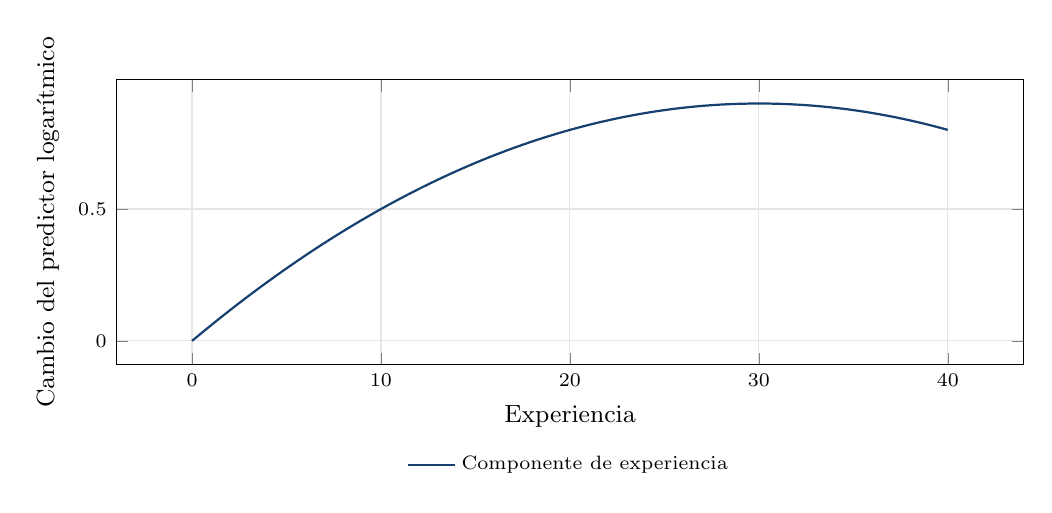
\begin{tikzpicture}
\begin{axis}[panelaxis,xlabel={Experiencia},ylabel={Cambio del predictor logarítmico},xtick={0,10,20,30,40}]
\addplot[azul,thick,no marks] coordinates {(0,0) (0.404040404,0.0240791756) (0.808080808,0.0478318539) (1.21212121,0.0712580349) (1.61616162,0.0943577186) (2.02020202,0.117130905) (2.42424242,0.139577594) (2.82828283,0.161697786) (3.23232323,0.18349148) (3.63636364,0.204958678) (4.04040404,0.226099378) (4.44444444,0.24691358) (4.84848485,0.267401286) (5.25252525,0.287562494) (5.65656566,0.307397204) (6.06060606,0.326905418) (6.46464646,0.346087134) (6.86868687,0.364942353) (7.27272727,0.383471074) (7.67676768,0.401673299) (8.08080808,0.419549026) (8.48484848,0.437098255) (8.88888889,0.454320988) (9.29292929,0.471217223) (9.6969697,0.487786961) (10.1010101,0.504030201) (10.5050505,0.519946944) (10.9090909,0.53553719) (11.3131313,0.550800939) (11.7171717,0.56573819) (12.1212121,0.580348944) (12.5252525,0.594633201) (12.9292929,0.60859096) (13.3333333,0.622222222) (13.7373737,0.635526987) (14.1414141,0.648505255) (14.5454545,0.661157025) (14.9494949,0.673482298) (15.3535354,0.685481073) (15.7575758,0.697153352) (16.1616162,0.708499133) (16.5656566,0.719518416) (16.969697,0.730211203) (17.3737374,0.740577492) (17.7777778,0.750617284) (18.1818182,0.760330579) (18.5858586,0.769717376) (18.989899,0.778777676) (19.3939394,0.787511478) (19.7979798,0.795918784) (20.2020202,0.803999592) (20.6060606,0.811753903) (21.010101,0.819181716) (21.4141414,0.826283032) (21.8181818,0.833057851) (22.2222222,0.839506173) (22.6262626,0.845627997) (23.030303,0.851423324) (23.4343434,0.856892154) (23.8383838,0.862034486) (24.2424242,0.866850321) (24.6464646,0.871339659) (25.0505051,0.8755025) (25.4545455,0.879338843) (25.8585859,0.882848689) (26.2626263,0.886032038) (26.6666667,0.888888889) (27.0707071,0.891419243) (27.4747475,0.8936231) (27.8787879,0.895500459) (28.2828283,0.897051321) (28.6868687,0.898275686) (29.0909091,0.899173554) (29.4949495,0.899744924) (29.8989899,0.899989797) (30.3030303,0.899908173) (30.7070707,0.899500051) (31.1111111,0.898765432) (31.5151515,0.897704316) (31.9191919,0.896316702) (32.3232323,0.894602592) (32.7272727,0.892561983) (33.1313131,0.890194878) (33.5353535,0.887501275) (33.9393939,0.884481175) (34.3434343,0.881134578) (34.7474747,0.877461484) (35.1515152,0.873461892) (35.5555556,0.869135802) (35.959596,0.864483216) (36.3636364,0.859504132) (36.7676768,0.854198551) (37.1717172,0.848566473) (37.5757576,0.842607897) (37.979798,0.836322824) (38.3838384,0.829711254) (38.7878788,0.822773186) (39.1919192,0.815508622) (39.5959596,0.807917559) (40,0.8)};
\addlegendentry{Componente de experiencia}
\end{axis}
\end{tikzpicture}
\caption{Con $\beta_r=0.06$ y $\beta_{rr}=-0.001$, el punto de giro del predictor es 30. La figura muestra una función especificada; su incertidumbre se calcula con la covarianza de ambos coeficientes.}\label{fig:panel-21}
\end{figure}
% FIN PANELFIG
\section{Una secuencia de análisis que conserva la pregunta}
Primero se define la unidad, el período y la población.
Después se verifica la variación temporal de cada variable y se especifica qué fuente de confusión controla cada efecto.
Se define la condición de exogeneidad, el estimador de pendiente y la unidad independiente para inferencia.
Finalmente se interpreta un contraste con su covarianza completa.
Esta secuencia conecta los números con un objeto económico identificable y evita sustituir la pregunta por una lista de comandos.



% MODULO 14_taller_fe.tex
\parte{XIV. Taller de FE: todos los números dentro de las matrices}
\section{Cómo usar las doce prácticas de efectos fijos}
Cada práctica tiene tres entidades, tres fechas y dos regresores; son nueve filas. Todos los datos son sintéticos. Se muestra el diseño completo por filas, cada desviación within, las ecuaciones normales y la matriz conjunta de covarianza. Para los momentos teóricos se adopta el modelo estático con errores independientes, media condicional cero y varianza conocida $\sigma^2=4$. La varianza residual estimada se calcula por separado. Las matrices decimales de covarianza se redondean a cinco cifras decimales; las expresiones con fracciones son exactas.

\section{Práctica FE 1: Tres fuentes de variación}
\begin{resuelto}{Tres fuentes de variación}
\textbf{Problema.} Distingue el nivel individual, la pendiente dentro y el error observado. Compara las pendientes pooled y FE; calcula la covarianza conjunta de pendientes e interceptos.

\begin{center}\small
\begin{tabular}{rrrrr}
\toprule
$i$&$t$&$x_{it,1}$&$x_{it,2}$&$y_{it}$\\
\midrule
1&1&3&2&2\\
1&2&8&3&6\\
1&3&2&1&1\\
2&1&5&1&7\\
2&2&8&-2&15\\
2&3&4&2&4\\
3&1&7&1&13\\
3&2&5&4&1\\
3&3&7&4&6\\
\bottomrule
\end{tabular}
\end{center}
\textbf{Modelo de construcción y modelo de incertidumbre.} Las pendientes generadoras de este conjunto son $\beta=\begin{pmatrix}
1\\-2
\end{pmatrix}$ y los interceptos $a=\begin{pmatrix}
2\\4\\6
\end{pmatrix}$. Los valores se construyeron agregando la siguiente realización sintética del error:
\[
\eps=\begin{pmatrix}
1\\2\\-1\\0\\-1\\0\\2\\-2\\1
\end{pmatrix}.
\]
La hipótesis de errores de media cero y varianza $4$ se adopta para calcular momentos teóricos; una única realización no permite verificarla.
\textbf{1. Medias individuales completas.}

\begin{center}\small
\begin{tabular}{rrrr}
\toprule
Entidad&$\bar x_{i,1}$&$\bar x_{i,2}$&$\bar y_i$\\
\midrule
1&$\frac{13}{3}$&2&3\\
2&$\frac{17}{3}$&$\frac{1}{3}$&$\frac{26}{3}$\\
3&$\frac{19}{3}$&3&$\frac{20}{3}$\\
\bottomrule
\end{tabular}
\end{center}
Cada media divide la suma de sus tres filas por $3$. Por ejemplo,
\[
\bar x_{1,1}=\frac{3+8+2}{3}=\frac{13}{3},\qquad \bar y_1=\frac{(2)+(6)+(1)}{3}=3.
\]
\textbf{2. Todas las filas transformadas.} Se resta la media de la entidad correspondiente, no la media global.

\begin{center}\small
\begin{tabular}{rrrrr}
\toprule
$i$&$t$&$\widetilde x_{it,1}$&$\widetilde x_{it,2}$&$\widetilde y_{it}$\\
\midrule
1&1&$-\frac{4}{3}$&$0$&$-1$\\
1&2&$\frac{11}{3}$&$1$&$3$\\
1&3&$-\frac{7}{3}$&$-1$&$-2$\\
2&1&$-\frac{2}{3}$&$\frac{2}{3}$&$-\frac{5}{3}$\\
2&2&$\frac{7}{3}$&$-\frac{7}{3}$&$\frac{19}{3}$\\
2&3&$-\frac{5}{3}$&$\frac{5}{3}$&$-\frac{14}{3}$\\
3&1&$\frac{2}{3}$&$-2$&$\frac{19}{3}$\\
3&2&$-\frac{4}{3}$&$1$&$-\frac{17}{3}$\\
3&3&$\frac{2}{3}$&$1$&$-\frac{2}{3}$\\
\bottomrule
\end{tabular}
\end{center}
\textbf{3. Sumatorias desplegadas.} El elemento cruzado de la matriz y el score de la primera columna son:
\[
\begin{aligned}
Q_{12}={}&(-\frac{4}{3})(0)+(\frac{11}{3})(1)+(-\frac{7}{3})(-1)\\{}&+(-\frac{2}{3})(\frac{2}{3})+(\frac{7}{3})(-\frac{7}{3})+(-\frac{5}{3})(\frac{5}{3})\\{}&+(\frac{2}{3})(-2)+(-\frac{4}{3})(1)+(\frac{2}{3})(1)\\{}={}&-\frac{14}{3}
\end{aligned}
\]
\[
\begin{aligned}
q_1={}&(-\frac{4}{3})(-1)+(\frac{11}{3})(3)+(-\frac{7}{3})(-2)\\{}&+(-\frac{2}{3})(-\frac{5}{3})+(\frac{7}{3})(\frac{19}{3})+(-\frac{5}{3})(-\frac{14}{3})\\{}&+(\frac{2}{3})(\frac{19}{3})+(-\frac{4}{3})(-\frac{17}{3})+(\frac{2}{3})(-\frac{2}{3})\\{}={}&52
\end{aligned}
\]
Los cuadrados de cada columna y el otro score completan el sistema:
\[
Q=\widetilde X\T\widetilde X=\begin{pmatrix}
32&-\frac{14}{3}\\-\frac{14}{3}&\frac{50}{3}
\end{pmatrix},\qquad q=\widetilde X\T\widetilde y=\begin{pmatrix}
52\\-\frac{113}{3}
\end{pmatrix}.
\]
\textbf{4. Inversa y pendientes.} El determinante es $\frac{4604}{9}>0$. Para una matriz simétrica de orden dos se intercambian las diagonales y se cambia el signo del cruzado:
\[
Q^{-1}=\begin{pmatrix}
\frac{75}{2302}&\frac{21}{2302}\\\frac{21}{2302}&\frac{72}{1151}
\end{pmatrix},\qquad
\widehat\beta=Q^{-1}q=\begin{pmatrix}
\frac{3109}{2302}\\-\frac{2166}{1151}
\end{pmatrix}.
\]
En la escala decimal, las pendientes son $1.35056$ y $-1.88184$. La diferencia realizada respecto de las pendientes generadoras es
\[
\widehat\beta-\beta=\begin{pmatrix}
\frac{807}{2302}\\\frac{136}{1151}
\end{pmatrix}=Q^{-1}\widetilde X\T\eps.
\]
\textbf{5. Interceptos y residuos completos.}
\[
\widehat a_{1}=3-(\frac{13}{3})(\frac{3109}{2302})-(2)(-\frac{2166}{1151})=\frac{6293}{6906}.
\]
\[
\widehat a_{2}=\frac{26}{3}-(\frac{17}{3})(\frac{3109}{2302})-(\frac{1}{3})(-\frac{2166}{1151})=\frac{3777}{2302}.
\]
\[
\widehat a_{3}=\frac{20}{3}-(\frac{19}{3})(\frac{3109}{2302})-(3)(-\frac{2166}{1151})=\frac{25957}{6906}.
\]

\begin{center}\small
\begin{tabular}{rrrrr}
\toprule
$i$&$t$&$\widehat y_{it}$&$\widehat\eps_{it}$&$\widehat\eps_{it}^{\,2}$\\
\midrule
1&1&1.19925&0.80075&0.64121\\
1&2&6.07023&-0.07023&0.00493\\
1&3&1.73052&-0.73052&0.53367\\
2&1&6.51173&0.48827&0.23841\\
2&2&16.20895&-1.20895&1.46156\\
2&3&3.27932&0.72068&0.51938\\
3&1&11.33073&1.66927&2.78647\\
3&2&2.98407&-1.98407&3.93654\\
3&3&5.6852&0.3148&0.0991\\
\bottomrule
\end{tabular}
\end{center}
Las ecuaciones normales dan $D\T\widehat\eps=0$ y $X\T\widehat\eps=0$. La suma de cuadrados es $\mathrm{SSE}\approx10.22126$; el rango del diseño completo es $3+2=5$, por lo que quedan $9-5=4$ grados de libertad y $s^2\approx2.55531$.
\textbf{6. Esperanzas y matriz completa de covarianza.} Bajo las hipótesis indicadas, $\E(\widehat\beta\mid X,a)=\beta$ y $\E(\widehat a\mid X,a)=a$. La covarianza de las pendientes, usando la varianza teórica $4$, es
\[
V_\beta=4Q^{-1}\approx\begin{pmatrix}
0.13032&0.03649\\0.03649&0.25022
\end{pmatrix}.
\]
En el orden $(\widehat a_1,\widehat a_2,\widehat a_3,\widehat\beta_1,\widehat\beta_2)$, la matriz conjunta es
\[
\Var\begin{pmatrix}\widehat a_1\\\widehat a_2\\\widehat a_3\\\widehat\beta_1\\\widehat\beta_2\end{pmatrix}
\approx\begin{pmatrix}
5.41384&3.83319&6.01448&-0.63771&-0.65856\\3.83319&5.68375&5.62467&-0.75065&-0.29018\\6.01448&5.62467&10.19925&-0.93484&-0.98175\\-0.63771&-0.75065&-0.93484&0.13032&0.03649\\-0.65856&-0.29018&-0.98175&0.03649&0.25022
\end{pmatrix}.
\]
Se obtuvo de $\Var(\widehat a)=4I_3/3+BV_\beta B\T$ y $\Cov(\widehat a,\widehat\beta)=-BV_\beta$, con $B$ formado por las medias. Es también $4([D,X]\T[D,X])^{-1}$; la equivalencia se verificó numéricamente.
\textbf{7. Contraste que necesita covarianza.} Para $l=\begin{pmatrix}
1\\1
\end{pmatrix}$, el efecto estimado es $l\T\widehat\beta\approx-0.53128$ y
\[
\Var(l\T\widehat\beta)=l\T V_\beta l\approx0.45352,\qquad \se(l\T\widehat\beta)\approx0.67344.
\]
La diferencia de interceptos $\widehat a_1-\widehat a_2\approx-0.72951$ tiene varianza $V_{a,11}+V_{a,22}-2V_{a,12}\approx3.43122$.
\textbf{8. Comparación y predicción.} Pooled con una constante produce pendientes aproximadamente $1.5856$ y $-1.59114$. FE produce las pendientes anteriores porque elimina los niveles individuales. La media ajustada de la primera fila es $\widehat a_1+x_{11}\T\widehat\beta\approx1.19925$; su varianza teórica es
\[
4/3+(x_{11}-\bar x_1)\T V_\beta(x_{11}-\bar x_1)\approx1.56502.
\]
Si se desea una covarianza clásica estimada, se reemplaza el $4$ por $s^2$ en todas las matrices esféricas: no se mezclan entradas provenientes de escalas distintas. Si se desea una covarianza agrupada, se construye otro meat con scores por entidad; no se obtiene cambiando solo ese escalar.
\end{resuelto}

\section{Práctica FE 2: Covarianza entre pendientes}
\begin{resuelto}{Covarianza entre pendientes}
\textbf{Problema.} Estudia dos regresores que no son ortogonales. Calcula la incertidumbre de la suma de sus pendientes utilizando el término fuera de diagonal.

\begin{center}\small
\begin{tabular}{rrrrr}
\toprule
$i$&$t$&$x_{it,1}$&$x_{it,2}$&$y_{it}$\\
\midrule
1&1&2&-1&9\\
1&2&3&-1&11\\
1&3&4&0&12\\
2&1&4&-1&13\\
2&2&3&1&9\\
2&3&7&0&20\\
3&1&2&3&10\\
3&2&6&4&16\\
3&3&1&-2&14\\
\bottomrule
\end{tabular}
\end{center}
\textbf{Modelo de construcción y modelo de incertidumbre.} Las pendientes generadoras de este conjunto son $\beta=\begin{pmatrix}
2\\-1
\end{pmatrix}$ y los interceptos $a=\begin{pmatrix}
2\\5\\8
\end{pmatrix}$. Los valores se construyeron agregando la siguiente realización sintética del error:
\[
\eps=\begin{pmatrix}
2\\2\\2\\-1\\-1\\1\\1\\0\\2
\end{pmatrix}.
\]
La hipótesis de errores de media cero y varianza $4$ se adopta para calcular momentos teóricos; una única realización no permite verificarla.
\textbf{1. Medias individuales completas.}

\begin{center}\small
\begin{tabular}{rrrr}
\toprule
Entidad&$\bar x_{i,1}$&$\bar x_{i,2}$&$\bar y_i$\\
\midrule
1&3&$-\frac{2}{3}$&$\frac{32}{3}$\\
2&$\frac{14}{3}$&0&14\\
3&3&$\frac{5}{3}$&$\frac{40}{3}$\\
\bottomrule
\end{tabular}
\end{center}
Cada media divide la suma de sus tres filas por $3$. Por ejemplo,
\[
\bar x_{1,1}=\frac{2+3+4}{3}=3,\qquad \bar y_1=\frac{(9)+(11)+(12)}{3}=\frac{32}{3}.
\]
\textbf{2. Todas las filas transformadas.} Se resta la media de la entidad correspondiente, no la media global.

\begin{center}\small
\begin{tabular}{rrrrr}
\toprule
$i$&$t$&$\widetilde x_{it,1}$&$\widetilde x_{it,2}$&$\widetilde y_{it}$\\
\midrule
1&1&$-1$&$-\frac{1}{3}$&$-\frac{5}{3}$\\
1&2&$0$&$-\frac{1}{3}$&$\frac{1}{3}$\\
1&3&$1$&$\frac{2}{3}$&$\frac{4}{3}$\\
2&1&$-\frac{2}{3}$&$-1$&$-1$\\
2&2&$-\frac{5}{3}$&$1$&$-5$\\
2&3&$\frac{7}{3}$&$0$&$6$\\
3&1&$-1$&$\frac{4}{3}$&$-\frac{10}{3}$\\
3&2&$3$&$\frac{7}{3}$&$\frac{8}{3}$\\
3&3&$-2$&$-\frac{11}{3}$&$\frac{2}{3}$\\
\bottomrule
\end{tabular}
\end{center}
\textbf{3. Sumatorias desplegadas.} El elemento cruzado de la matriz y el score de la primera columna son:
\[
\begin{aligned}
Q_{12}={}&(-1)(-\frac{1}{3})+(0)(-\frac{1}{3})+(1)(\frac{2}{3})\\{}&+(-\frac{2}{3})(-1)+(-\frac{5}{3})(1)+(\frac{7}{3})(0)\\{}&+(-1)(\frac{4}{3})+(3)(\frac{7}{3})+(-2)(-\frac{11}{3})\\{}={}&13
\end{aligned}
\]
\[
\begin{aligned}
q_1={}&(-1)(-\frac{5}{3})+(0)(\frac{1}{3})+(1)(\frac{4}{3})\\{}&+(-\frac{2}{3})(-1)+(-\frac{5}{3})(-5)+(\frac{7}{3})(6)\\{}&+(-1)(-\frac{10}{3})+(3)(\frac{8}{3})+(-2)(\frac{2}{3})\\{}={}&36
\end{aligned}
\]
Los cuadrados de cada columna y el otro score completan el sistema:
\[
Q=\widetilde X\T\widetilde X=\begin{pmatrix}
\frac{74}{3}&13\\13&\frac{70}{3}
\end{pmatrix},\qquad q=\widetilde X\T\widetilde y=\begin{pmatrix}
36\\-\frac{10}{3}
\end{pmatrix}.
\]
\textbf{4. Inversa y pendientes.} El determinante es $\frac{3659}{9}>0$. Para una matriz simétrica de orden dos se intercambian las diagonales y se cambia el signo del cruzado:
\[
Q^{-1}=\begin{pmatrix}
\frac{210}{3659}&-\frac{117}{3659}\\-\frac{117}{3659}&\frac{222}{3659}
\end{pmatrix},\qquad
\widehat\beta=Q^{-1}q=\begin{pmatrix}
\frac{7950}{3659}\\-\frac{4952}{3659}
\end{pmatrix}.
\]
En la escala decimal, las pendientes son $2.17272$ y $-1.35338$. La diferencia realizada respecto de las pendientes generadoras es
\[
\widehat\beta-\beta=\begin{pmatrix}
\frac{632}{3659}\\-\frac{1293}{3659}
\end{pmatrix}=Q^{-1}\widetilde X\T\eps.
\]
\textbf{5. Interceptos y residuos completos.}
\[
\widehat a_{1}=\frac{32}{3}-(3)(\frac{7950}{3659})-(-\frac{2}{3})(-\frac{4952}{3659})=\frac{11878}{3659}.
\]
\[
\widehat a_{2}=14-(\frac{14}{3})(\frac{7950}{3659})-(0)(-\frac{4952}{3659})=\frac{14126}{3659}.
\]
\[
\widehat a_{3}=\frac{40}{3}-(3)(\frac{7950}{3659})-(\frac{5}{3})(-\frac{4952}{3659})=\frac{33190}{3659}.
\]

\begin{center}\small
\begin{tabular}{rrrrr}
\toprule
$i$&$t$&$\widehat y_{it}$&$\widehat\eps_{it}$&$\widehat\eps_{it}^{\,2}$\\
\midrule
1&1&8.94507&0.05493&0.00302\\
1&2&11.11779&-0.11779&0.01387\\
1&3&11.93714&0.06286&0.00395\\
2&1&13.90489&-0.90489&0.81883\\
2&2&9.02542&-0.02542&0.00065\\
2&3&19.06969&0.93031&0.86547\\
3&1&9.35611&0.64389&0.4146\\
3&2&16.69363&-0.69363&0.48113\\
3&3&13.95026&0.04974&0.00247\\
\bottomrule
\end{tabular}
\end{center}
Las ecuaciones normales dan $D\T\widehat\eps=0$ y $X\T\widehat\eps=0$. La suma de cuadrados es $\mathrm{SSE}\approx2.60399$; el rango del diseño completo es $3+2=5$, por lo que quedan $9-5=4$ grados de libertad y $s^2\approx0.651$.
\textbf{6. Esperanzas y matriz completa de covarianza.} Bajo las hipótesis indicadas, $\E(\widehat\beta\mid X,a)=\beta$ y $\E(\widehat a\mid X,a)=a$. La covarianza de las pendientes, usando la varianza teórica $4$, es
\[
V_\beta=4Q^{-1}\approx\begin{pmatrix}
0.22957&-0.1279\\-0.1279&0.24269
\end{pmatrix}.
\]
En el orden $(\widehat a_1,\widehat a_2,\widehat a_3,\widehat\beta_1,\widehat\beta_2)$, la matriz conjunta es
\[
\Var\begin{pmatrix}\widehat a_1\\\widehat a_2\\\widehat a_3\\\widehat\beta_1\\\widehat\beta_2\end{pmatrix}
\approx\begin{pmatrix}
4.01895&3.61192&1.41277&-0.77398&0.5455\\3.61192&6.33288&2.21919&-1.07133&0.59688\\1.41277&2.21919&2.79457&-0.47554&-0.02077\\-0.77398&-1.07133&-0.47554&0.22957&-0.1279\\0.5455&0.59688&-0.02077&-0.1279&0.24269
\end{pmatrix}.
\]
Se obtuvo de $\Var(\widehat a)=4I_3/3+BV_\beta B\T$ y $\Cov(\widehat a,\widehat\beta)=-BV_\beta$, con $B$ formado por las medias. Es también $4([D,X]\T[D,X])^{-1}$; la equivalencia se verificó numéricamente.
\textbf{7. Contraste que necesita covarianza.} Para $l=\begin{pmatrix}
1\\-2
\end{pmatrix}$, el efecto estimado es $l\T\widehat\beta\approx4.87948$ y
\[
\Var(l\T\widehat\beta)=l\T V_\beta l\approx1.71194,\qquad \se(l\T\widehat\beta)\approx1.30841.
\]
La diferencia de interceptos $\widehat a_1-\widehat a_2\approx-0.61438$ tiene varianza $V_{a,11}+V_{a,22}-2V_{a,12}\approx3.12799$.
\textbf{8. Comparación y predicción.} Pooled con una constante produce pendientes aproximadamente $1.57393$ y $-0.43243$. FE produce las pendientes anteriores porque elimina los niveles individuales. La media ajustada de la primera fila es $\widehat a_1+x_{11}\T\widehat\beta\approx8.94507$; su varianza teórica es
\[
4/3+(x_{11}-\bar x_1)\T V_\beta(x_{11}-\bar x_1)\approx1.5046.
\]
Si se desea una covarianza clásica estimada, se reemplaza el $4$ por $s^2$ en todas las matrices esféricas: no se mezclan entradas provenientes de escalas distintas. Si se desea una covarianza agrupada, se construye otro meat con scores por entidad; no se obtiene cambiando solo ese escalar.
\end{resuelto}

\section{Práctica FE 3: Una pendiente negativa}
\begin{resuelto}{Una pendiente negativa}
\textbf{Problema.} Interpreta una columna cuyo coeficiente es negativo y verifica que restar medias no cambia el signo de la variable por una regla general.

\begin{center}\small
\begin{tabular}{rrrrr}
\toprule
$i$&$t$&$x_{it,1}$&$x_{it,2}$&$y_{it}$\\
\midrule
1&1&3&-1&15\\
1&2&7&-3&31\\
1&3&8&3&22\\
2&1&3&3&7\\
2&2&8&1&28\\
2&3&1&4&-1\\
3&1&4&0&21\\
3&2&2&-2&21\\
3&3&5&2&22\\
\bottomrule
\end{tabular}
\end{center}
\textbf{Modelo de construcción y modelo de incertidumbre.} Las pendientes generadoras de este conjunto son $\beta=\begin{pmatrix}
3\\-2
\end{pmatrix}$ y los interceptos $a=\begin{pmatrix}
2\\6\\10
\end{pmatrix}$. Los valores se construyeron agregando la siguiente realización sintética del error:
\[
\eps=\begin{pmatrix}
2\\2\\2\\-2\\0\\-2\\-1\\1\\1
\end{pmatrix}.
\]
La hipótesis de errores de media cero y varianza $4$ se adopta para calcular momentos teóricos; una única realización no permite verificarla.
\textbf{1. Medias individuales completas.}

\begin{center}\small
\begin{tabular}{rrrr}
\toprule
Entidad&$\bar x_{i,1}$&$\bar x_{i,2}$&$\bar y_i$\\
\midrule
1&6&$-\frac{1}{3}$&$\frac{68}{3}$\\
2&4&$\frac{8}{3}$&$\frac{34}{3}$\\
3&$\frac{11}{3}$&0&$\frac{64}{3}$\\
\bottomrule
\end{tabular}
\end{center}
Cada media divide la suma de sus tres filas por $3$. Por ejemplo,
\[
\bar x_{1,1}=\frac{3+7+8}{3}=6,\qquad \bar y_1=\frac{(15)+(31)+(22)}{3}=\frac{68}{3}.
\]
\textbf{2. Todas las filas transformadas.} Se resta la media de la entidad correspondiente, no la media global.

\begin{center}\small
\begin{tabular}{rrrrr}
\toprule
$i$&$t$&$\widetilde x_{it,1}$&$\widetilde x_{it,2}$&$\widetilde y_{it}$\\
\midrule
1&1&$-3$&$-\frac{2}{3}$&$-\frac{23}{3}$\\
1&2&$1$&$-\frac{8}{3}$&$\frac{25}{3}$\\
1&3&$2$&$\frac{10}{3}$&$-\frac{2}{3}$\\
2&1&$-1$&$\frac{1}{3}$&$-\frac{13}{3}$\\
2&2&$4$&$-\frac{5}{3}$&$\frac{50}{3}$\\
2&3&$-3$&$\frac{4}{3}$&$-\frac{37}{3}$\\
3&1&$\frac{1}{3}$&$0$&$-\frac{1}{3}$\\
3&2&$-\frac{5}{3}$&$-2$&$-\frac{1}{3}$\\
3&3&$\frac{4}{3}$&$2$&$\frac{2}{3}$\\
\bottomrule
\end{tabular}
\end{center}
\textbf{3. Sumatorias desplegadas.} El elemento cruzado de la matriz y el score de la primera columna son:
\[
\begin{aligned}
Q_{12}={}&(-3)(-\frac{2}{3})+(1)(-\frac{8}{3})+(2)(\frac{10}{3})\\{}&+(-1)(\frac{1}{3})+(4)(-\frac{5}{3})+(-3)(\frac{4}{3})\\{}&+(\frac{1}{3})(0)+(-\frac{5}{3})(-2)+(\frac{4}{3})(2)\\{}={}&1
\end{aligned}
\]
\[
\begin{aligned}
q_1={}&(-3)(-\frac{23}{3})+(1)(\frac{25}{3})+(2)(-\frac{2}{3})\\{}&+(-1)(-\frac{13}{3})+(4)(\frac{50}{3})+(-3)(-\frac{37}{3})\\{}&+(\frac{1}{3})(-\frac{1}{3})+(-\frac{5}{3})(-\frac{1}{3})+(\frac{4}{3})(\frac{2}{3})\\{}={}&\frac{418}{3}
\end{aligned}
\]
Los cuadrados de cada columna y el otro score completan el sistema:
\[
Q=\widetilde X\T\widetilde X=\begin{pmatrix}
\frac{134}{3}&1\\1&\frac{94}{3}
\end{pmatrix},\qquad q=\widetilde X\T\widetilde y=\begin{pmatrix}
\frac{418}{3}\\-63
\end{pmatrix}.
\]
\textbf{4. Inversa y pendientes.} El determinante es $\frac{12587}{9}>0$. Para una matriz simétrica de orden dos se intercambian las diagonales y se cambia el signo del cruzado:
\[
Q^{-1}=\begin{pmatrix}
\frac{282}{12587}&-\frac{9}{12587}\\-\frac{9}{12587}&\frac{402}{12587}
\end{pmatrix},\qquad
\widehat\beta=Q^{-1}q=\begin{pmatrix}
\frac{39859}{12587}\\-\frac{26580}{12587}
\end{pmatrix}.
\]
En la escala decimal, las pendientes son $3.16668$ y $-2.1117$. La diferencia realizada respecto de las pendientes generadoras es
\[
\widehat\beta-\beta=\begin{pmatrix}
\frac{2098}{12587}\\-\frac{1406}{12587}
\end{pmatrix}=Q^{-1}\widetilde X\T\eps.
\]
\textbf{5. Interceptos y residuos completos.}
\[
\widehat a_{1}=\frac{68}{3}-(6)(\frac{39859}{12587})-(-\frac{1}{3})(-\frac{26580}{12587})=\frac{111874}{37761}.
\]
\[
\widehat a_{2}=\frac{34}{3}-(4)(\frac{39859}{12587})-(\frac{8}{3})(-\frac{26580}{12587})=\frac{162290}{37761}.
\]
\[
\widehat a_{3}=\frac{64}{3}-(\frac{11}{3})(\frac{39859}{12587})-(0)(-\frac{26580}{12587})=\frac{122373}{12587}.
\]

\begin{center}\small
\begin{tabular}{rrrrr}
\toprule
$i$&$t$&$\widehat y_{it}$&$\widehat\eps_{it}$&$\widehat\eps_{it}^{\,2}$\\
\midrule
1&1&14.57443&0.42557&0.18111\\
1&2&31.46455&-0.46455&0.21581\\
1&3&21.96102&0.03898&0.00152\\
2&1&7.46275&-0.46275&0.21414\\
2&2&27.51956&0.48044&0.23083\\
2&3&-0.98231&-0.01769&0.00031\\
3&1&22.38889&-1.38889&1.92902\\
3&2&20.27894&0.72106&0.51993\\
3&3&21.33217&0.66783&0.446\\
\bottomrule
\end{tabular}
\end{center}
Las ecuaciones normales dan $D\T\widehat\eps=0$ y $X\T\widehat\eps=0$. La suma de cuadrados es $\mathrm{SSE}\approx3.73867$; el rango del diseño completo es $3+2=5$, por lo que quedan $9-5=4$ grados de libertad y $s^2\approx0.93467$.
\textbf{6. Esperanzas y matriz completa de covarianza.} Bajo las hipótesis indicadas, $\E(\widehat\beta\mid X,a)=\beta$ y $\E(\widehat a\mid X,a)=a$. La covarianza de las pendientes, usando la varianza teórica $4$, es
\[
V_\beta=4Q^{-1}\approx\begin{pmatrix}
0.08962&-0.00286\\-0.00286&0.12775
\end{pmatrix}.
\]
En el orden $(\widehat a_1,\widehat a_2,\widehat a_3,\widehat\beta_1,\widehat\beta_2)$, la matriz conjunta es
\[
\Var\begin{pmatrix}\widehat a_1\\\widehat a_2\\\widehat a_3\\\widehat\beta_1\\\widehat\beta_2\end{pmatrix}
\approx\begin{pmatrix}
4.58515&1.99529&1.97505&-0.53865&0.05974\\1.99529&3.61463&1.28641&-0.35084&-0.32923\\1.97505&1.28641&2.53817&-0.32859&0.01049\\-0.53865&-0.35084&-0.32859&0.08962&-0.00286\\0.05974&-0.32923&0.01049&-0.00286&0.12775
\end{pmatrix}.
\]
Se obtuvo de $\Var(\widehat a)=4I_3/3+BV_\beta B\T$ y $\Cov(\widehat a,\widehat\beta)=-BV_\beta$, con $B$ formado por las medias. Es también $4([D,X]\T[D,X])^{-1}$; la equivalencia se verificó numéricamente.
\textbf{7. Contraste que necesita covarianza.} Para $l=\begin{pmatrix}
2\\-1
\end{pmatrix}$, el efecto estimado es $l\T\widehat\beta\approx8.44506$ y
\[
\Var(l\T\widehat\beta)=l\T V_\beta l\approx0.49766,\qquad \se(l\T\widehat\beta)\approx0.70545.
\]
La diferencia de interceptos $\widehat a_1-\widehat a_2\approx-1.33513$ tiene varianza $V_{a,11}+V_{a,22}-2V_{a,12}\approx4.20921$.
\textbf{8. Comparación y predicción.} Pooled con una constante produce pendientes aproximadamente $2.77401$ y $-2.32463$. FE produce las pendientes anteriores porque elimina los niveles individuales. La media ajustada de la primera fila es $\widehat a_1+x_{11}\T\widehat\beta\approx14.57443$; su varianza teórica es
\[
4/3+(x_{11}-\bar x_1)\T V_\beta(x_{11}-\bar x_1)\approx2.18522.
\]
Si se desea una covarianza clásica estimada, se reemplaza el $4$ por $s^2$ en todas las matrices esféricas: no se mezclan entradas provenientes de escalas distintas. Si se desea una covarianza agrupada, se construye otro meat con scores por entidad; no se obtiene cambiando solo ese escalar.
\end{resuelto}

\section{Práctica FE 4: Un contraste de pendientes}
\begin{resuelto}{Un contraste de pendientes}
\textbf{Problema.} Calcula el contraste de la primera pendiente menos dos veces la segunda. Distingue la combinación del coeficiente y la combinación de sus varianzas.

\begin{center}\small
\begin{tabular}{rrrrr}
\toprule
$i$&$t$&$x_{it,1}$&$x_{it,2}$&$y_{it}$\\
\midrule
1&1&6&-3&12\\
1&2&5&1&7\\
1&3&8&-2&14\\
2&1&7&-1&11\\
2&2&2&-3&8\\
2&3&5&0&6\\
3&1&5&-1&11\\
3&2&2&3&1\\
3&3&4&4&2\\
\bottomrule
\end{tabular}
\end{center}
\textbf{Modelo de construcción y modelo de incertidumbre.} Las pendientes generadoras de este conjunto son $\beta=\begin{pmatrix}
1\\-1
\end{pmatrix}$ y los interceptos $a=\begin{pmatrix}
2\\3\\4
\end{pmatrix}$. Los valores se construyeron agregando la siguiente realización sintética del error:
\[
\eps=\begin{pmatrix}
1\\1\\2\\0\\0\\-2\\1\\-2\\-2
\end{pmatrix}.
\]
La hipótesis de errores de media cero y varianza $4$ se adopta para calcular momentos teóricos; una única realización no permite verificarla.
\textbf{1. Medias individuales completas.}

\begin{center}\small
\begin{tabular}{rrrr}
\toprule
Entidad&$\bar x_{i,1}$&$\bar x_{i,2}$&$\bar y_i$\\
\midrule
1&$\frac{19}{3}$&$-\frac{4}{3}$&11\\
2&$\frac{14}{3}$&$-\frac{4}{3}$&$\frac{25}{3}$\\
3&$\frac{11}{3}$&2&$\frac{14}{3}$\\
\bottomrule
\end{tabular}
\end{center}
Cada media divide la suma de sus tres filas por $3$. Por ejemplo,
\[
\bar x_{1,1}=\frac{6+5+8}{3}=\frac{19}{3},\qquad \bar y_1=\frac{(12)+(7)+(14)}{3}=11.
\]
\textbf{2. Todas las filas transformadas.} Se resta la media de la entidad correspondiente, no la media global.

\begin{center}\small
\begin{tabular}{rrrrr}
\toprule
$i$&$t$&$\widetilde x_{it,1}$&$\widetilde x_{it,2}$&$\widetilde y_{it}$\\
\midrule
1&1&$-\frac{1}{3}$&$-\frac{5}{3}$&$1$\\
1&2&$-\frac{4}{3}$&$\frac{7}{3}$&$-4$\\
1&3&$\frac{5}{3}$&$-\frac{2}{3}$&$3$\\
2&1&$\frac{7}{3}$&$\frac{1}{3}$&$\frac{8}{3}$\\
2&2&$-\frac{8}{3}$&$-\frac{5}{3}$&$-\frac{1}{3}$\\
2&3&$\frac{1}{3}$&$\frac{4}{3}$&$-\frac{7}{3}$\\
3&1&$\frac{4}{3}$&$-3$&$\frac{19}{3}$\\
3&2&$-\frac{5}{3}$&$1$&$-\frac{11}{3}$\\
3&3&$\frac{1}{3}$&$2$&$-\frac{8}{3}$\\
\bottomrule
\end{tabular}
\end{center}
\textbf{3. Sumatorias desplegadas.} El elemento cruzado de la matriz y el score de la primera columna son:
\[
\begin{aligned}
Q_{12}={}&(-\frac{1}{3})(-\frac{5}{3})+(-\frac{4}{3})(\frac{7}{3})+(\frac{5}{3})(-\frac{2}{3})\\{}&+(\frac{7}{3})(\frac{1}{3})+(-\frac{8}{3})(-\frac{5}{3})+(\frac{1}{3})(\frac{4}{3})\\{}&+(\frac{4}{3})(-3)+(-\frac{5}{3})(1)+(\frac{1}{3})(2)\\{}={}&-3
\end{aligned}
\]
\[
\begin{aligned}
q_1={}&(-\frac{1}{3})(1)+(-\frac{4}{3})(-4)+(\frac{5}{3})(3)\\{}&+(\frac{7}{3})(\frac{8}{3})+(-\frac{8}{3})(-\frac{1}{3})+(\frac{1}{3})(-\frac{7}{3})\\{}&+(\frac{4}{3})(\frac{19}{3})+(-\frac{5}{3})(-\frac{11}{3})+(\frac{1}{3})(-\frac{8}{3})\\{}={}&30
\end{aligned}
\]
Los cuadrados de cada columna y el otro score completan el sistema:
\[
Q=\widetilde X\T\widetilde X=\begin{pmatrix}
22&-3\\-3&\frac{82}{3}
\end{pmatrix},\qquad q=\widetilde X\T\widetilde y=\begin{pmatrix}
30\\-\frac{128}{3}
\end{pmatrix}.
\]
\textbf{4. Inversa y pendientes.} El determinante es $\frac{1777}{3}>0$. Para una matriz simétrica de orden dos se intercambian las diagonales y se cambia el signo del cruzado:
\[
Q^{-1}=\begin{pmatrix}
\frac{82}{1777}&\frac{9}{1777}\\\frac{9}{1777}&\frac{66}{1777}
\end{pmatrix},\qquad
\widehat\beta=Q^{-1}q=\begin{pmatrix}
\frac{2076}{1777}\\-\frac{2546}{1777}
\end{pmatrix}.
\]
En la escala decimal, las pendientes son $1.16826$ y $-1.43275$. La diferencia realizada respecto de las pendientes generadoras es
\[
\widehat\beta-\beta=\begin{pmatrix}
\frac{299}{1777}\\-\frac{769}{1777}
\end{pmatrix}=Q^{-1}\widetilde X\T\eps.
\]
\textbf{5. Interceptos y residuos completos.}
\[
\widehat a_{1}=11-(\frac{19}{3})(\frac{2076}{1777})-(-\frac{4}{3})(-\frac{2546}{1777})=\frac{9013}{5331}.
\]
\[
\widehat a_{2}=\frac{25}{3}-(\frac{14}{3})(\frac{2076}{1777})-(-\frac{4}{3})(-\frac{2546}{1777})=\frac{5177}{5331}.
\]
\[
\widehat a_{3}=\frac{14}{3}-(\frac{11}{3})(\frac{2076}{1777})-(2)(-\frac{2546}{1777})=\frac{17318}{5331}.
\]

\begin{center}\small
\begin{tabular}{rrrrr}
\toprule
$i$&$t$&$\widehat y_{it}$&$\widehat\eps_{it}$&$\widehat\eps_{it}^{\,2}$\\
\midrule
1&1&12.9985&-0.9985&0.997\\
1&2&6.09923&0.90077&0.81138\\
1&3&13.90227&0.09773&0.00955\\
2&1&10.58169&0.41831&0.17498\\
2&2&7.60589&0.39411&0.15532\\
2&3&6.81242&-0.81242&0.66002\\
3&1&10.5226&0.4774&0.22791\\
3&2&1.28681&-0.28681&0.08226\\
3&3&2.19058&-0.19058&0.03632\\
\bottomrule
\end{tabular}
\end{center}
Las ecuaciones normales dan $D\T\widehat\eps=0$ y $X\T\widehat\eps=0$. La suma de cuadrados es $\mathrm{SSE}\approx3.15476$; el rango del diseño completo es $3+2=5$, por lo que quedan $9-5=4$ grados de libertad y $s^2\approx0.78869$.
\textbf{6. Esperanzas y matriz completa de covarianza.} Bajo las hipótesis indicadas, $\E(\widehat\beta\mid X,a)=\beta$ y $\E(\widehat a\mid X,a)=a$. La covarianza de las pendientes, usando la varianza teórica $4$, es
\[
V_\beta=4Q^{-1}\approx\begin{pmatrix}
0.18458&0.02026\\0.02026&0.14856
\end{pmatrix}.
\]
En el orden $(\widehat a_1,\widehat a_2,\widehat a_3,\widehat\beta_1,\widehat\beta_2)$, la matriz conjunta es
\[
\Var\begin{pmatrix}\widehat a_1\\\widehat a_2\\\widehat a_3\\\widehat\beta_1\\\widehat\beta_2\end{pmatrix}
\approx\begin{pmatrix}
8.65904&5.42237&4.04777&-1.142&0.06978\\5.42237&5.3651&2.85225&-0.83437&0.10355\\4.04777&2.85225&4.70631&-0.71731&-0.37141\\-1.142&-0.83437&-0.71731&0.18458&0.02026\\0.06978&0.10355&-0.37141&0.02026&0.14856
\end{pmatrix}.
\]
Se obtuvo de $\Var(\widehat a)=4I_3/3+BV_\beta B\T$ y $\Cov(\widehat a,\widehat\beta)=-BV_\beta$, con $B$ formado por las medias. Es también $4([D,X]\T[D,X])^{-1}$; la equivalencia se verificó numéricamente.
\textbf{7. Contraste que necesita covarianza.} Para $l=\begin{pmatrix}
1\\1
\end{pmatrix}$, el efecto estimado es $l\T\widehat\beta\approx-0.26449$ y
\[
\Var(l\T\widehat\beta)=l\T V_\beta l\approx0.37366,\qquad \se(l\T\widehat\beta)\approx0.61128.
\]
La diferencia de interceptos $\widehat a_1-\widehat a_2\approx0.71956$ tiene varianza $V_{a,11}+V_{a,22}-2V_{a,12}\approx3.17939$.
\textbf{8. Comparación y predicción.} Pooled con una constante produce pendientes aproximadamente $1.12199$ y $-1.18899$. FE produce las pendientes anteriores porque elimina los niveles individuales. La media ajustada de la primera fila es $\widehat a_1+x_{11}\T\widehat\beta\approx12.9985$; su varianza teórica es
\[
4/3+(x_{11}-\bar x_1)\T V_\beta(x_{11}-\bar x_1)\approx1.78903.
\]
Si se desea una covarianza clásica estimada, se reemplaza el $4$ por $s^2$ en todas las matrices esféricas: no se mezclan entradas provenientes de escalas distintas. Si se desea una covarianza agrupada, se construye otro meat con scores por entidad; no se obtiene cambiando solo ese escalar.
\end{resuelto}

\section{Práctica FE 5: Medias alejadas de cero}
\begin{resuelto}{Medias alejadas de cero}
\textbf{Problema.} Examina por qué la incertidumbre del intercepto depende de las medias de los regresores, aun si la pendiente within es precisa.

\begin{center}\small
\begin{tabular}{rrrrr}
\toprule
$i$&$t$&$x_{it,1}$&$x_{it,2}$&$y_{it}$\\
\midrule
1&1&5&0&13\\
1&2&8&-1&22\\
1&3&5&-2&14\\
2&1&2&-1&12\\
2&2&4&0&12\\
2&3&7&1&17\\
3&1&8&-3&26\\
3&2&2&-2&14\\
3&3&1&0&8\\
\bottomrule
\end{tabular}
\end{center}
\textbf{Modelo de construcción y modelo de incertidumbre.} Las pendientes generadoras de este conjunto son $\beta=\begin{pmatrix}
2\\-2
\end{pmatrix}$ y los interceptos $a=\begin{pmatrix}
2\\4\\6
\end{pmatrix}$. Los valores se construyeron agregando la siguiente realización sintética del error:
\[
\eps=\begin{pmatrix}
1\\2\\-2\\2\\0\\1\\-2\\0\\0
\end{pmatrix}.
\]
La hipótesis de errores de media cero y varianza $4$ se adopta para calcular momentos teóricos; una única realización no permite verificarla.
\textbf{1. Medias individuales completas.}

\begin{center}\small
\begin{tabular}{rrrr}
\toprule
Entidad&$\bar x_{i,1}$&$\bar x_{i,2}$&$\bar y_i$\\
\midrule
1&6&-1&$\frac{49}{3}$\\
2&$\frac{13}{3}$&0&$\frac{41}{3}$\\
3&$\frac{11}{3}$&$-\frac{5}{3}$&16\\
\bottomrule
\end{tabular}
\end{center}
Cada media divide la suma de sus tres filas por $3$. Por ejemplo,
\[
\bar x_{1,1}=\frac{5+8+5}{3}=6,\qquad \bar y_1=\frac{(13)+(22)+(14)}{3}=\frac{49}{3}.
\]
\textbf{2. Todas las filas transformadas.} Se resta la media de la entidad correspondiente, no la media global.

\begin{center}\small
\begin{tabular}{rrrrr}
\toprule
$i$&$t$&$\widetilde x_{it,1}$&$\widetilde x_{it,2}$&$\widetilde y_{it}$\\
\midrule
1&1&$-1$&$1$&$-\frac{10}{3}$\\
1&2&$2$&$0$&$\frac{17}{3}$\\
1&3&$-1$&$-1$&$-\frac{7}{3}$\\
2&1&$-\frac{7}{3}$&$-1$&$-\frac{5}{3}$\\
2&2&$-\frac{1}{3}$&$0$&$-\frac{5}{3}$\\
2&3&$\frac{8}{3}$&$1$&$\frac{10}{3}$\\
3&1&$\frac{13}{3}$&$-\frac{4}{3}$&$10$\\
3&2&$-\frac{5}{3}$&$-\frac{1}{3}$&$-2$\\
3&3&$-\frac{8}{3}$&$\frac{5}{3}$&$-8$\\
\bottomrule
\end{tabular}
\end{center}
\textbf{3. Sumatorias desplegadas.} El elemento cruzado de la matriz y el score de la primera columna son:
\[
\begin{aligned}
Q_{12}={}&(-1)(1)+(2)(0)+(-1)(-1)\\{}&+(-\frac{7}{3})(-1)+(-\frac{1}{3})(0)+(\frac{8}{3})(1)\\{}&+(\frac{13}{3})(-\frac{4}{3})+(-\frac{5}{3})(-\frac{1}{3})+(-\frac{8}{3})(\frac{5}{3})\\{}={}&-\frac{14}{3}
\end{aligned}
\]
\[
\begin{aligned}
q_1={}&(-1)(-\frac{10}{3})+(2)(\frac{17}{3})+(-1)(-\frac{7}{3})\\{}&+(-\frac{7}{3})(-\frac{5}{3})+(-\frac{1}{3})(-\frac{5}{3})+(\frac{8}{3})(\frac{10}{3})\\{}&+(\frac{13}{3})(10)+(-\frac{5}{3})(-2)+(-\frac{8}{3})(-8)\\{}={}&\frac{295}{3}
\end{aligned}
\]
Los cuadrados de cada columna y el otro score completan el sistema:
\[
Q=\widetilde X\T\widetilde X=\begin{pmatrix}
\frac{142}{3}&-\frac{14}{3}\\-\frac{14}{3}&\frac{26}{3}
\end{pmatrix},\qquad q=\widetilde X\T\widetilde y=\begin{pmatrix}
\frac{295}{3}\\-22
\end{pmatrix}.
\]
\textbf{4. Inversa y pendientes.} El determinante es $\frac{3496}{9}>0$. Para una matriz simétrica de orden dos se intercambian las diagonales y se cambia el signo del cruzado:
\[
Q^{-1}=\begin{pmatrix}
\frac{39}{1748}&\frac{21}{1748}\\\frac{21}{1748}&\frac{213}{1748}
\end{pmatrix},\qquad
\widehat\beta=Q^{-1}q=\begin{pmatrix}
\frac{3373}{1748}\\-\frac{2621}{1748}
\end{pmatrix}.
\]
En la escala decimal, las pendientes son $1.92963$ y $-1.49943$. La diferencia realizada respecto de las pendientes generadoras es
\[
\widehat\beta-\beta=\begin{pmatrix}
-\frac{123}{1748}\\\frac{875}{1748}
\end{pmatrix}=Q^{-1}\widetilde X\T\eps.
\]
\textbf{5. Interceptos y residuos completos.}
\[
\widehat a_{1}=\frac{49}{3}-(6)(\frac{3373}{1748})-(-1)(-\frac{2621}{1748})=\frac{17075}{5244}.
\]
\[
\widehat a_{2}=\frac{41}{3}-(\frac{13}{3})(\frac{3373}{1748})-(0)(-\frac{2621}{1748})=\frac{9273}{1748}.
\]
\[
\widehat a_{3}=16-(\frac{11}{3})(\frac{3373}{1748})-(-\frac{5}{3})(-\frac{2621}{1748})=\frac{2808}{437}.
\]

\begin{center}\small
\begin{tabular}{rrrrr}
\toprule
$i$&$t$&$\widehat y_{it}$&$\widehat\eps_{it}$&$\widehat\eps_{it}^{\,2}$\\
\midrule
1&1&12.90427&0.09573&0.00916\\
1&2&20.1926&1.8074&3.26669\\
1&3&15.90313&-1.90313&3.62189\\
2&1&10.66362&1.33638&1.78592\\
2&2&13.02346&-1.02346&1.04746\\
2&3&17.31293&-0.31293&0.09792\\
3&1&26.36098&-0.36098&0.13031\\
3&2&13.28375&0.71625&0.51301\\
3&3&8.35526&-0.35526&0.12621\\
\bottomrule
\end{tabular}
\end{center}
Las ecuaciones normales dan $D\T\widehat\eps=0$ y $X\T\widehat\eps=0$. La suma de cuadrados es $\mathrm{SSE}\approx10.59859$; el rango del diseño completo es $3+2=5$, por lo que quedan $9-5=4$ grados de libertad y $s^2\approx2.64965$.
\textbf{6. Esperanzas y matriz completa de covarianza.} Bajo las hipótesis indicadas, $\E(\widehat\beta\mid X,a)=\beta$ y $\E(\widehat a\mid X,a)=a$. La covarianza de las pendientes, usando la varianza teórica $4$, es
\[
V_\beta=4Q^{-1}\approx\begin{pmatrix}
0.08924&0.04805\\0.04805&0.48741
\end{pmatrix}.
\]
En el orden $(\widehat a_1,\widehat a_2,\widehat a_3,\widehat\beta_1,\widehat\beta_2)$, la matriz conjunta es
\[
\Var\begin{pmatrix}\widehat a_1\\\widehat a_2\\\widehat a_3\\\widehat\beta_1\\\widehat\beta_2\end{pmatrix}
\approx\begin{pmatrix}
4.4569&2.11213&2.11899&-0.48741&0.19908\\2.11213&3.00915&1.07094&-0.38673&-0.20824\\2.11899&1.07094&3.29977&-0.24714&0.63616\\-0.48741&-0.38673&-0.24714&0.08924&0.04805\\0.19908&-0.20824&0.63616&0.04805&0.48741
\end{pmatrix}.
\]
Se obtuvo de $\Var(\widehat a)=4I_3/3+BV_\beta B\T$ y $\Cov(\widehat a,\widehat\beta)=-BV_\beta$, con $B$ formado por las medias. Es también $4([D,X]\T[D,X])^{-1}$; la equivalencia se verificó numéricamente.
\textbf{7. Contraste que necesita covarianza.} Para $l=\begin{pmatrix}
1\\-2
\end{pmatrix}$, el efecto estimado es $l\T\widehat\beta\approx4.92849$ y
\[
\Var(l\T\widehat\beta)=l\T V_\beta l\approx1.84668,\qquad \se(l\T\widehat\beta)\approx1.35893.
\]
La diferencia de interceptos $\widehat a_1-\widehat a_2\approx-2.04882$ tiene varianza $V_{a,11}+V_{a,22}-2V_{a,12}\approx3.2418$.
\textbf{8. Comparación y predicción.} Pooled con una constante produce pendientes aproximadamente $1.70933$ y $-1.712$. FE produce las pendientes anteriores porque elimina los niveles individuales. La media ajustada de la primera fila es $\widehat a_1+x_{11}\T\widehat\beta\approx12.90427$; su varianza teórica es
\[
4/3+(x_{11}-\bar x_1)\T V_\beta(x_{11}-\bar x_1)\approx1.81388.
\]
Si se desea una covarianza clásica estimada, se reemplaza el $4$ por $s^2$ en todas las matrices esféricas: no se mezclan entradas provenientes de escalas distintas. Si se desea una covarianza agrupada, se construye otro meat con scores por entidad; no se obtiene cambiando solo ese escalar.
\end{resuelto}

\section{Práctica FE 6: Recuperar niveles}
\begin{resuelto}{Recuperar niveles}
\textbf{Problema.} Construye las predicciones de una entidad existente y compara su varianza con la de su intercepto aislado.

\begin{center}\small
\begin{tabular}{rrrrr}
\toprule
$i$&$t$&$x_{it,1}$&$x_{it,2}$&$y_{it}$\\
\midrule
1&1&5&4&15\\
1&2&7&2&23\\
1&3&6&-3&22\\
2&1&4&-2&20\\
2&2&2&3&9\\
2&3&8&-3&34\\
3&1&1&3&7\\
3&2&3&4&15\\
3&3&7&2&28\\
\bottomrule
\end{tabular}
\end{center}
\textbf{Modelo de construcción y modelo de incertidumbre.} Las pendientes generadoras de este conjunto son $\beta=\begin{pmatrix}
3\\-1
\end{pmatrix}$ y los interceptos $a=\begin{pmatrix}
2\\5\\8
\end{pmatrix}$. Los valores se construyeron agregando la siguiente realización sintética del error:
\[
\eps=\begin{pmatrix}
2\\2\\-1\\1\\1\\2\\-1\\2\\1
\end{pmatrix}.
\]
La hipótesis de errores de media cero y varianza $4$ se adopta para calcular momentos teóricos; una única realización no permite verificarla.
\textbf{1. Medias individuales completas.}

\begin{center}\small
\begin{tabular}{rrrr}
\toprule
Entidad&$\bar x_{i,1}$&$\bar x_{i,2}$&$\bar y_i$\\
\midrule
1&6&1&20\\
2&$\frac{14}{3}$&$-\frac{2}{3}$&21\\
3&$\frac{11}{3}$&3&$\frac{50}{3}$\\
\bottomrule
\end{tabular}
\end{center}
Cada media divide la suma de sus tres filas por $3$. Por ejemplo,
\[
\bar x_{1,1}=\frac{5+7+6}{3}=6,\qquad \bar y_1=\frac{(15)+(23)+(22)}{3}=20.
\]
\textbf{2. Todas las filas transformadas.} Se resta la media de la entidad correspondiente, no la media global.

\begin{center}\small
\begin{tabular}{rrrrr}
\toprule
$i$&$t$&$\widetilde x_{it,1}$&$\widetilde x_{it,2}$&$\widetilde y_{it}$\\
\midrule
1&1&$-1$&$3$&$-5$\\
1&2&$1$&$1$&$3$\\
1&3&$0$&$-4$&$2$\\
2&1&$-\frac{2}{3}$&$-\frac{4}{3}$&$-1$\\
2&2&$-\frac{8}{3}$&$\frac{11}{3}$&$-12$\\
2&3&$\frac{10}{3}$&$-\frac{7}{3}$&$13$\\
3&1&$-\frac{8}{3}$&$0$&$-\frac{29}{3}$\\
3&2&$-\frac{2}{3}$&$1$&$-\frac{5}{3}$\\
3&3&$\frac{10}{3}$&$-1$&$\frac{34}{3}$\\
\bottomrule
\end{tabular}
\end{center}
\textbf{3. Sumatorias desplegadas.} El elemento cruzado de la matriz y el score de la primera columna son:
\[
\begin{aligned}
Q_{12}={}&(-1)(3)+(1)(1)+(0)(-4)\\{}&+(-\frac{2}{3})(-\frac{4}{3})+(-\frac{8}{3})(\frac{11}{3})+(\frac{10}{3})(-\frac{7}{3})\\{}&+(-\frac{8}{3})(0)+(-\frac{2}{3})(1)+(\frac{10}{3})(-1)\\{}={}&-\frac{68}{3}
\end{aligned}
\]
\[
\begin{aligned}
q_1={}&(-1)(-5)+(1)(3)+(0)(2)\\{}&+(-\frac{2}{3})(-1)+(-\frac{8}{3})(-12)+(\frac{10}{3})(13)\\{}&+(-\frac{8}{3})(-\frac{29}{3})+(-\frac{2}{3})(-\frac{5}{3})+(\frac{10}{3})(\frac{34}{3})\\{}={}&\frac{446}{3}
\end{aligned}
\]
Los cuadrados de cada columna y el otro score completan el sistema:
\[
Q=\widetilde X\T\widetilde X=\begin{pmatrix}
\frac{118}{3}&-\frac{68}{3}\\-\frac{68}{3}&\frac{146}{3}
\end{pmatrix},\qquad q=\widetilde X\T\widetilde y=\begin{pmatrix}
\frac{446}{3}\\-106
\end{pmatrix}.
\]
\textbf{4. Inversa y pendientes.} El determinante es $\frac{12604}{9}>0$. Para una matriz simétrica de orden dos se intercambian las diagonales y se cambia el signo del cruzado:
\[
Q^{-1}=\begin{pmatrix}
\frac{219}{6302}&\frac{51}{3151}\\\frac{51}{3151}&\frac{177}{6302}
\end{pmatrix},\qquad
\widehat\beta=Q^{-1}q=\begin{pmatrix}
\frac{10873}{3151}\\-\frac{1799}{3151}
\end{pmatrix}.
\]
En la escala decimal, las pendientes son $3.45065$ y $-0.57093$. La diferencia realizada respecto de las pendientes generadoras es
\[
\widehat\beta-\beta=\begin{pmatrix}
\frac{1420}{3151}\\\frac{1352}{3151}
\end{pmatrix}=Q^{-1}\widetilde X\T\eps.
\]
\textbf{5. Interceptos y residuos completos.}
\[
\widehat a_{1}=20-(6)(\frac{10873}{3151})-(1)(-\frac{1799}{3151})=-\frac{419}{3151}.
\]
\[
\widehat a_{2}=21-(\frac{14}{3})(\frac{10873}{3151})-(-\frac{2}{3})(-\frac{1799}{3151})=\frac{14231}{3151}.
\]
\[
\widehat a_{3}=\frac{50}{3}-(\frac{11}{3})(\frac{10873}{3151})-(3)(-\frac{1799}{3151})=\frac{18046}{3151}.
\]

\begin{center}\small
\begin{tabular}{rrrrr}
\toprule
$i$&$t$&$\widehat y_{it}$&$\widehat\eps_{it}$&$\widehat\eps_{it}^{\,2}$\\
\midrule
1&1&14.83656&0.16344&0.02671\\
1&2&22.87972&0.12028&0.01447\\
1&3&22.28372&-0.28372&0.0805\\
2&1&19.46081&0.53919&0.29073\\
2&2&9.70486&-0.70486&0.49682\\
2&3&33.83434&0.16566&0.02744\\
3&1&7.46493&-0.46493&0.21616\\
3&2&13.7953&1.2047&1.45129\\
3&3&28.73977&-0.73977&0.54725\\
\bottomrule
\end{tabular}
\end{center}
Las ecuaciones normales dan $D\T\widehat\eps=0$ y $X\T\widehat\eps=0$. La suma de cuadrados es $\mathrm{SSE}\approx3.15138$; el rango del diseño completo es $3+2=5$, por lo que quedan $9-5=4$ grados de libertad y $s^2\approx0.78785$.
\textbf{6. Esperanzas y matriz completa de covarianza.} Bajo las hipótesis indicadas, $\E(\widehat\beta\mid X,a)=\beta$ y $\E(\widehat a\mid X,a)=a$. La covarianza de las pendientes, usando la varianza teórica $4$, es
\[
V_\beta=4Q^{-1}\approx\begin{pmatrix}
0.139&0.06474\\0.06474&0.11235
\end{pmatrix}.
\]
En el orden $(\widehat a_1,\widehat a_2,\widehat a_3,\widehat\beta_1,\widehat\beta_2)$, la matriz conjunta es
\[
\Var\begin{pmatrix}\widehat a_1\\\widehat a_2\\\widehat a_3\\\widehat\beta_1\\\widehat\beta_2\end{pmatrix}
\approx\begin{pmatrix}
7.2267&3.86036&4.79784&-0.89876&-0.50079\\3.86036&4.00762&2.90194&-0.60552&-0.22723\\4.79784&2.90194&5.63758&-0.7039&-0.57442\\-0.89876&-0.60552&-0.7039&0.139&0.06474\\-0.50079&-0.22723&-0.57442&0.06474&0.11235
\end{pmatrix}.
\]
Se obtuvo de $\Var(\widehat a)=4I_3/3+BV_\beta B\T$ y $\Cov(\widehat a,\widehat\beta)=-BV_\beta$, con $B$ formado por las medias. Es también $4([D,X]\T[D,X])^{-1}$; la equivalencia se verificó numéricamente.
\textbf{7. Contraste que necesita covarianza.} Para $l=\begin{pmatrix}
2\\-1
\end{pmatrix}$, el efecto estimado es $l\T\widehat\beta\approx7.47223$ y
\[
\Var(l\T\widehat\beta)=l\T V_\beta l\approx0.40939,\qquad \se(l\T\widehat\beta)\approx0.63984.
\]
La diferencia de interceptos $\widehat a_1-\widehat a_2\approx-4.64932$ tiene varianza $V_{a,11}+V_{a,22}-2V_{a,12}\approx3.51359$.
\textbf{8. Comparación y predicción.} Pooled con una constante produce pendientes aproximadamente $2.9562$ y $-0.65539$. FE produce las pendientes anteriores porque elimina los niveles individuales. La media ajustada de la primera fila es $\widehat a_1+x_{11}\T\widehat\beta\approx14.83656$; su varianza teórica es
\[
4/3+(x_{11}-\bar x_1)\T V_\beta(x_{11}-\bar x_1)\approx2.095.
\]
Si se desea una covarianza clásica estimada, se reemplaza el $4$ por $s^2$ en todas las matrices esféricas: no se mezclan entradas provenientes de escalas distintas. Si se desea una covarianza agrupada, se construye otro meat con scores por entidad; no se obtiene cambiando solo ese escalar.
\end{resuelto}

\section{Práctica FE 7: Un cambio simultáneo}
\begin{resuelto}{Un cambio simultáneo}
\textbf{Problema.} Estudia un aumento de dos unidades en la primera variable y una disminución de una unidad en la segunda.

\begin{center}\small
\begin{tabular}{rrrrr}
\toprule
$i$&$t$&$x_{it,1}$&$x_{it,2}$&$y_{it}$\\
\midrule
1&1&1&3&-5\\
1&2&3&-1&9\\
1&3&3&0&6\\
2&1&4&1&8\\
2&2&7&3&9\\
2&3&8&0&14\\
3&1&7&-1&18\\
3&2&5&-3&22\\
3&3&6&2&14\\
\bottomrule
\end{tabular}
\end{center}
\textbf{Modelo de construcción y modelo de incertidumbre.} Las pendientes generadoras de este conjunto son $\beta=\begin{pmatrix}
1\\-2
\end{pmatrix}$ y los interceptos $a=\begin{pmatrix}
2\\6\\10
\end{pmatrix}$. Los valores se construyeron agregando la siguiente realización sintética del error:
\[
\eps=\begin{pmatrix}
-2\\2\\1\\0\\2\\0\\-1\\1\\2
\end{pmatrix}.
\]
La hipótesis de errores de media cero y varianza $4$ se adopta para calcular momentos teóricos; una única realización no permite verificarla.
\textbf{1. Medias individuales completas.}

\begin{center}\small
\begin{tabular}{rrrr}
\toprule
Entidad&$\bar x_{i,1}$&$\bar x_{i,2}$&$\bar y_i$\\
\midrule
1&$\frac{7}{3}$&$\frac{2}{3}$&$\frac{10}{3}$\\
2&$\frac{19}{3}$&$\frac{4}{3}$&$\frac{31}{3}$\\
3&6&$-\frac{2}{3}$&18\\
\bottomrule
\end{tabular}
\end{center}
Cada media divide la suma de sus tres filas por $3$. Por ejemplo,
\[
\bar x_{1,1}=\frac{1+3+3}{3}=\frac{7}{3},\qquad \bar y_1=\frac{(-5)+(9)+(6)}{3}=\frac{10}{3}.
\]
\textbf{2. Todas las filas transformadas.} Se resta la media de la entidad correspondiente, no la media global.

\begin{center}\small
\begin{tabular}{rrrrr}
\toprule
$i$&$t$&$\widetilde x_{it,1}$&$\widetilde x_{it,2}$&$\widetilde y_{it}$\\
\midrule
1&1&$-\frac{4}{3}$&$\frac{7}{3}$&$-\frac{25}{3}$\\
1&2&$\frac{2}{3}$&$-\frac{5}{3}$&$\frac{17}{3}$\\
1&3&$\frac{2}{3}$&$-\frac{2}{3}$&$\frac{8}{3}$\\
2&1&$-\frac{7}{3}$&$-\frac{1}{3}$&$-\frac{7}{3}$\\
2&2&$\frac{2}{3}$&$\frac{5}{3}$&$-\frac{4}{3}$\\
2&3&$\frac{5}{3}$&$-\frac{4}{3}$&$\frac{11}{3}$\\
3&1&$1$&$-\frac{1}{3}$&$0$\\
3&2&$-1$&$-\frac{7}{3}$&$4$\\
3&3&$0$&$\frac{8}{3}$&$-4$\\
\bottomrule
\end{tabular}
\end{center}
\textbf{3. Sumatorias desplegadas.} El elemento cruzado de la matriz y el score de la primera columna son:
\[
\begin{aligned}
Q_{12}={}&(-\frac{4}{3})(\frac{7}{3})+(\frac{2}{3})(-\frac{5}{3})+(\frac{2}{3})(-\frac{2}{3})\\{}&+(-\frac{7}{3})(-\frac{1}{3})+(\frac{2}{3})(\frac{5}{3})+(\frac{5}{3})(-\frac{4}{3})\\{}&+(1)(-\frac{1}{3})+(-1)(-\frac{7}{3})+(0)(\frac{8}{3})\\{}={}&-3
\end{aligned}
\]
\[
\begin{aligned}
q_1={}&(-\frac{4}{3})(-\frac{25}{3})+(\frac{2}{3})(\frac{17}{3})+(\frac{2}{3})(\frac{8}{3})\\{}&+(-\frac{7}{3})(-\frac{7}{3})+(\frac{2}{3})(-\frac{4}{3})+(\frac{5}{3})(\frac{11}{3})\\{}&+(1)(0)+(-1)(4)+(0)(-4)\\{}={}&\frac{70}{3}
\end{aligned}
\]
Los cuadrados de cada columna y el otro score completan el sistema:
\[
Q=\widetilde X\T\widetilde X=\begin{pmatrix}
\frac{40}{3}&-3\\-3&26
\end{pmatrix},\qquad q=\widetilde X\T\widetilde y=\begin{pmatrix}
\frac{70}{3}\\-57
\end{pmatrix}.
\]
\textbf{4. Inversa y pendientes.} El determinante es $\frac{1013}{3}>0$. Para una matriz simétrica de orden dos se intercambian las diagonales y se cambia el signo del cruzado:
\[
Q^{-1}=\begin{pmatrix}
\frac{78}{1013}&\frac{9}{1013}\\\frac{9}{1013}&\frac{40}{1013}
\end{pmatrix},\qquad
\widehat\beta=Q^{-1}q=\begin{pmatrix}
\frac{1307}{1013}\\-\frac{2070}{1013}
\end{pmatrix}.
\]
En la escala decimal, las pendientes son $1.29023$ y $-2.04344$. La diferencia realizada respecto de las pendientes generadoras es
\[
\widehat\beta-\beta=\begin{pmatrix}
\frac{294}{1013}\\-\frac{44}{1013}
\end{pmatrix}=Q^{-1}\widetilde X\T\eps.
\]
\textbf{5. Interceptos y residuos completos.}
\[
\widehat a_{1}=\frac{10}{3}-(\frac{7}{3})(\frac{1307}{1013})-(\frac{2}{3})(-\frac{2070}{1013})=\frac{1707}{1013}.
\]
\[
\widehat a_{2}=\frac{31}{3}-(\frac{19}{3})(\frac{1307}{1013})-(\frac{4}{3})(-\frac{2070}{1013})=\frac{4950}{1013}.
\]
\[
\widehat a_{3}=18-(6)(\frac{1307}{1013})-(-\frac{2}{3})(-\frac{2070}{1013})=\frac{9012}{1013}.
\]

\begin{center}\small
\begin{tabular}{rrrrr}
\toprule
$i$&$t$&$\widehat y_{it}$&$\widehat\eps_{it}$&$\widehat\eps_{it}^{\,2}$\\
\midrule
1&1&-3.15499&-1.84501&3.40408\\
1&2&7.59921&1.40079&1.96221\\
1&3&5.55577&0.44423&0.19734\\
2&1&8.00395&-0.00395&0.00002\\
2&2&7.78776&1.21224&1.46953\\
2&3&15.20829&-1.20829&1.45997\\
3&1&19.97137&-1.97137&3.88631\\
3&2&21.47779&0.52221&0.2727\\
3&3&12.55084&1.44916&2.10007\\
\bottomrule
\end{tabular}
\end{center}
Las ecuaciones normales dan $D\T\widehat\eps=0$ y $X\T\widehat\eps=0$. La suma de cuadrados es $\mathrm{SSE}\approx14.75222$; el rango del diseño completo es $3+2=5$, por lo que quedan $9-5=4$ grados de libertad y $s^2\approx3.68806$.
\textbf{6. Esperanzas y matriz completa de covarianza.} Bajo las hipótesis indicadas, $\E(\widehat\beta\mid X,a)=\beta$ y $\E(\widehat a\mid X,a)=a$. La covarianza de las pendientes, usando la varianza teórica $4$, es
\[
V_\beta=4Q^{-1}\approx\begin{pmatrix}
0.308&0.03554\\0.03554&0.15795
\end{pmatrix}.
\]
En el orden $(\widehat a_1,\widehat a_2,\widehat a_3,\widehat\beta_1,\widehat\beta_2)$, la matriz conjunta es
\[
\Var\begin{pmatrix}\widehat a_1\\\widehat a_2\\\widehat a_3\\\widehat\beta_1\\\widehat\beta_2\end{pmatrix}
\approx\begin{pmatrix}
3.19096&4.95251&4.32862&-0.74235&-0.18822\\4.95251&14.56839&11.69771&-1.99803&-0.43567\\4.32862&11.69771&12.20709&-1.82428&-0.10793\\-0.74235&-1.99803&-1.82428&0.308&0.03554\\-0.18822&-0.43567&-0.10793&0.03554&0.15795
\end{pmatrix}.
\]
Se obtuvo de $\Var(\widehat a)=4I_3/3+BV_\beta B\T$ y $\Cov(\widehat a,\widehat\beta)=-BV_\beta$, con $B$ formado por las medias. Es también $4([D,X]\T[D,X])^{-1}$; la equivalencia se verificó numéricamente.
\textbf{7. Contraste que necesita covarianza.} Para $l=\begin{pmatrix}
1\\1
\end{pmatrix}$, el efecto estimado es $l\T\widehat\beta\approx-0.75321$ y
\[
\Var(l\T\widehat\beta)=l\T V_\beta l\approx0.53702,\qquad \se(l\T\widehat\beta)\approx0.73282.
\]
La diferencia de interceptos $\widehat a_1-\widehat a_2\approx-3.20138$ tiene varianza $V_{a,11}+V_{a,22}-2V_{a,12}\approx7.85434$.
\textbf{8. Comparación y predicción.} Pooled con una constante produce pendientes aproximadamente $2.13574$ y $-2.40495$. FE produce las pendientes anteriores porque elimina los niveles individuales. La media ajustada de la primera fila es $\widehat a_1+x_{11}\T\widehat\beta\approx-3.15499$; su varianza teórica es
\[
4/3+(x_{11}-\bar x_1)\T V_\beta(x_{11}-\bar x_1)\approx2.51969.
\]
Si se desea una covarianza clásica estimada, se reemplaza el $4$ por $s^2$ en todas las matrices esféricas: no se mezclan entradas provenientes de escalas distintas. Si se desea una covarianza agrupada, se construye otro meat con scores por entidad; no se obtiene cambiando solo ese escalar.
\end{resuelto}

\section{Práctica FE 8: La matriz de efectos}
\begin{resuelto}{La matriz de efectos}
\textbf{Problema.} Verifica directamente la igualdad LSDV--within y cuenta todos los grados de libertad residuales.

\begin{center}\small
\begin{tabular}{rrrrr}
\toprule
$i$&$t$&$x_{it,1}$&$x_{it,2}$&$y_{it}$\\
\midrule
1&1&8&4&15\\
1&2&8&3&13\\
1&3&7&3&11\\
2&1&6&2&13\\
2&2&8&3&18\\
2&3&2&1&8\\
3&1&1&4&2\\
3&2&5&4&8\\
3&3&7&-1&21\\
\bottomrule
\end{tabular}
\end{center}
\textbf{Modelo de construcción y modelo de incertidumbre.} Las pendientes generadoras de este conjunto son $\beta=\begin{pmatrix}
2\\-1
\end{pmatrix}$ y los interceptos $a=\begin{pmatrix}
2\\3\\4
\end{pmatrix}$. Los valores se construyeron agregando la siguiente realización sintética del error:
\[
\eps=\begin{pmatrix}
1\\-2\\-2\\0\\2\\2\\0\\-2\\2
\end{pmatrix}.
\]
La hipótesis de errores de media cero y varianza $4$ se adopta para calcular momentos teóricos; una única realización no permite verificarla.
\textbf{1. Medias individuales completas.}

\begin{center}\small
\begin{tabular}{rrrr}
\toprule
Entidad&$\bar x_{i,1}$&$\bar x_{i,2}$&$\bar y_i$\\
\midrule
1&$\frac{23}{3}$&$\frac{10}{3}$&13\\
2&$\frac{16}{3}$&2&13\\
3&$\frac{13}{3}$&$\frac{7}{3}$&$\frac{31}{3}$\\
\bottomrule
\end{tabular}
\end{center}
Cada media divide la suma de sus tres filas por $3$. Por ejemplo,
\[
\bar x_{1,1}=\frac{8+8+7}{3}=\frac{23}{3},\qquad \bar y_1=\frac{(15)+(13)+(11)}{3}=13.
\]
\textbf{2. Todas las filas transformadas.} Se resta la media de la entidad correspondiente, no la media global.

\begin{center}\small
\begin{tabular}{rrrrr}
\toprule
$i$&$t$&$\widetilde x_{it,1}$&$\widetilde x_{it,2}$&$\widetilde y_{it}$\\
\midrule
1&1&$\frac{1}{3}$&$\frac{2}{3}$&$2$\\
1&2&$\frac{1}{3}$&$-\frac{1}{3}$&$0$\\
1&3&$-\frac{2}{3}$&$-\frac{1}{3}$&$-2$\\
2&1&$\frac{2}{3}$&$0$&$0$\\
2&2&$\frac{8}{3}$&$1$&$5$\\
2&3&$-\frac{10}{3}$&$-1$&$-5$\\
3&1&$-\frac{10}{3}$&$\frac{5}{3}$&$-\frac{25}{3}$\\
3&2&$\frac{2}{3}$&$\frac{5}{3}$&$-\frac{7}{3}$\\
3&3&$\frac{8}{3}$&$-\frac{10}{3}$&$\frac{32}{3}$\\
\bottomrule
\end{tabular}
\end{center}
\textbf{3. Sumatorias desplegadas.} El elemento cruzado de la matriz y el score de la primera columna son:
\[
\begin{aligned}
Q_{12}={}&(\frac{1}{3})(\frac{2}{3})+(\frac{1}{3})(-\frac{1}{3})+(-\frac{2}{3})(-\frac{1}{3})\\{}&+(\frac{2}{3})(0)+(\frac{8}{3})(1)+(-\frac{10}{3})(-1)\\{}&+(-\frac{10}{3})(\frac{5}{3})+(\frac{2}{3})(\frac{5}{3})+(\frac{8}{3})(-\frac{10}{3})\\{}={}&-7
\end{aligned}
\]
\[
\begin{aligned}
q_1={}&(\frac{1}{3})(2)+(\frac{1}{3})(0)+(-\frac{2}{3})(-2)\\{}&+(\frac{2}{3})(0)+(\frac{8}{3})(5)+(-\frac{10}{3})(-5)\\{}&+(-\frac{10}{3})(-\frac{25}{3})+(\frac{2}{3})(-\frac{7}{3})+(\frac{8}{3})(\frac{32}{3})\\{}={}&\frac{260}{3}
\end{aligned}
\]
Los cuadrados de cada columna y el otro score completan el sistema:
\[
Q=\widetilde X\T\widetilde X=\begin{pmatrix}
38&-7\\-7&\frac{58}{3}
\end{pmatrix},\qquad q=\widetilde X\T\widetilde y=\begin{pmatrix}
\frac{260}{3}\\-\frac{124}{3}
\end{pmatrix}.
\]
\textbf{4. Inversa y pendientes.} El determinante es $\frac{2057}{3}>0$. Para una matriz simétrica de orden dos se intercambian las diagonales y se cambia el signo del cruzado:
\[
Q^{-1}=\begin{pmatrix}
\frac{58}{2057}&\frac{21}{2057}\\\frac{21}{2057}&\frac{114}{2057}
\end{pmatrix},\qquad
\widehat\beta=Q^{-1}q=\begin{pmatrix}
\frac{12476}{6171}\\-\frac{2892}{2057}
\end{pmatrix}.
\]
En la escala decimal, las pendientes son $2.02171$ y $-1.40593$. La diferencia realizada respecto de las pendientes generadoras es
\[
\widehat\beta-\beta=\begin{pmatrix}
\frac{134}{6171}\\-\frac{835}{2057}
\end{pmatrix}=Q^{-1}\widetilde X\T\eps.
\]
\textbf{5. Interceptos y residuos completos.}
\[
\widehat a_{1}=13-(\frac{23}{3})(\frac{12476}{6171})-(\frac{10}{3})(-\frac{2892}{2057})=\frac{40481}{18513}.
\]
\[
\widehat a_{2}=13-(\frac{16}{3})(\frac{12476}{6171})-(2)(-\frac{2892}{2057})=\frac{5477}{1089}.
\]
\[
\widehat a_{3}=\frac{31}{3}-(\frac{13}{3})(\frac{12476}{6171})-(\frac{7}{3})(-\frac{2892}{2057})=\frac{5285}{1089}.
\]

\begin{center}\small
\begin{tabular}{rrrrr}
\toprule
$i$&$t$&$\widehat y_{it}$&$\widehat\eps_{it}$&$\widehat\eps_{it}^{\,2}$\\
\midrule
1&1&12.73662&2.26338&5.1229\\
1&2&14.14255&-1.14255&1.30542\\
1&3&12.12083&-1.12083&1.25627\\
2&1&14.34781&-1.34781&1.81659\\
2&2&16.98531&1.01469&1.0296\\
2&3&7.66688&0.33312&0.11097\\
3&1&1.25107&0.74893&0.5609\\
3&2&9.33792&-1.33792&1.79004\\
3&3&20.41101&0.58899&0.34691\\
\bottomrule
\end{tabular}
\end{center}
Las ecuaciones normales dan $D\T\widehat\eps=0$ y $X\T\widehat\eps=0$. La suma de cuadrados es $\mathrm{SSE}\approx13.3396$; el rango del diseño completo es $3+2=5$, por lo que quedan $9-5=4$ grados de libertad y $s^2\approx3.3349$.
\textbf{6. Esperanzas y matriz completa de covarianza.} Bajo las hipótesis indicadas, $\E(\widehat\beta\mid X,a)=\beta$ y $\E(\widehat a\mid X,a)=a$. La covarianza de las pendientes, usando la varianza teórica $4$, es
\[
V_\beta=4Q^{-1}\approx\begin{pmatrix}
0.11279&0.04084\\0.04084&0.22168
\end{pmatrix}.
\]
En el orden $(\widehat a_1,\widehat a_2,\widehat a_3,\widehat\beta_1,\widehat\beta_2)$, la matriz conjunta es
\[
\Var\begin{pmatrix}\widehat a_1\\\widehat a_2\\\widehat a_3\\\widehat\beta_1\\\widehat\beta_2\end{pmatrix}
\approx\begin{pmatrix}
12.51294&7.44169&6.79155&-1.00081&-1.05202\\7.44169&6.29936&4.50321&-0.6832&-0.66116\\6.79155&4.50321&5.48393&-0.58402&-0.69421\\-1.00081&-0.6832&-0.58402&0.11279&0.04084\\-1.05202&-0.66116&-0.69421&0.04084&0.22168
\end{pmatrix}.
\]
Se obtuvo de $\Var(\widehat a)=4I_3/3+BV_\beta B\T$ y $\Cov(\widehat a,\widehat\beta)=-BV_\beta$, con $B$ formado por las medias. Es también $4([D,X]\T[D,X])^{-1}$; la equivalencia se verificó numéricamente.
\textbf{7. Contraste que necesita covarianza.} Para $l=\begin{pmatrix}
1\\-2
\end{pmatrix}$, el efecto estimado es $l\T\widehat\beta\approx4.83358$ y
\[
\Var(l\T\widehat\beta)=l\T V_\beta l\approx0.83617,\qquad \se(l\T\widehat\beta)\approx0.91442.
\]
La diferencia de interceptos $\widehat a_1-\widehat a_2\approx-2.84276$ tiene varianza $V_{a,11}+V_{a,22}-2V_{a,12}\approx3.92891$.
\textbf{8. Comparación y predicción.} Pooled con una constante produce pendientes aproximadamente $1.74063$ y $-1.71037$. FE produce las pendientes anteriores porque elimina los niveles individuales. La media ajustada de la primera fila es $\widehat a_1+x_{11}\T\widehat\beta\approx12.73662$; su varianza teórica es
\[
4/3+(x_{11}-\bar x_1)\T V_\beta(x_{11}-\bar x_1)\approx1.46254.
\]
Si se desea una covarianza clásica estimada, se reemplaza el $4$ por $s^2$ en todas las matrices esféricas: no se mezclan entradas provenientes de escalas distintas. Si se desea una covarianza agrupada, se construye otro meat con scores por entidad; no se obtiene cambiando solo ese escalar.
\end{resuelto}

\section{Práctica FE 9: Una diferencia de interceptos}
\begin{resuelto}{Una diferencia de interceptos}
\textbf{Problema.} Calcula la incertidumbre de una diferencia de niveles individuales, reconociendo que los interceptos estimados comparten las pendientes.

\begin{center}\small
\begin{tabular}{rrrrr}
\toprule
$i$&$t$&$x_{it,1}$&$x_{it,2}$&$y_{it}$\\
\midrule
1&1&6&-2&22\\
1&2&3&2&6\\
1&3&5&2&15\\
2&1&5&3&15\\
2&2&4&3&12\\
2&3&6&-1&26\\
3&1&8&2&28\\
3&2&1&3&1\\
3&3&7&-3&35\\
\bottomrule
\end{tabular}
\end{center}
\textbf{Modelo de construcción y modelo de incertidumbre.} Las pendientes generadoras de este conjunto son $\beta=\begin{pmatrix}
3\\-2
\end{pmatrix}$ y los interceptos $a=\begin{pmatrix}
2\\4\\6
\end{pmatrix}$. Los valores se construyeron agregando la siguiente realización sintética del error:
\[
\eps=\begin{pmatrix}
-2\\-1\\2\\2\\2\\2\\2\\-2\\2
\end{pmatrix}.
\]
La hipótesis de errores de media cero y varianza $4$ se adopta para calcular momentos teóricos; una única realización no permite verificarla.
\textbf{1. Medias individuales completas.}

\begin{center}\small
\begin{tabular}{rrrr}
\toprule
Entidad&$\bar x_{i,1}$&$\bar x_{i,2}$&$\bar y_i$\\
\midrule
1&$\frac{14}{3}$&$\frac{2}{3}$&$\frac{43}{3}$\\
2&5&$\frac{5}{3}$&$\frac{53}{3}$\\
3&$\frac{16}{3}$&$\frac{2}{3}$&$\frac{64}{3}$\\
\bottomrule
\end{tabular}
\end{center}
Cada media divide la suma de sus tres filas por $3$. Por ejemplo,
\[
\bar x_{1,1}=\frac{6+3+5}{3}=\frac{14}{3},\qquad \bar y_1=\frac{(22)+(6)+(15)}{3}=\frac{43}{3}.
\]
\textbf{2. Todas las filas transformadas.} Se resta la media de la entidad correspondiente, no la media global.

\begin{center}\small
\begin{tabular}{rrrrr}
\toprule
$i$&$t$&$\widetilde x_{it,1}$&$\widetilde x_{it,2}$&$\widetilde y_{it}$\\
\midrule
1&1&$\frac{4}{3}$&$-\frac{8}{3}$&$\frac{23}{3}$\\
1&2&$-\frac{5}{3}$&$\frac{4}{3}$&$-\frac{25}{3}$\\
1&3&$\frac{1}{3}$&$\frac{4}{3}$&$\frac{2}{3}$\\
2&1&$0$&$\frac{4}{3}$&$-\frac{8}{3}$\\
2&2&$-1$&$\frac{4}{3}$&$-\frac{17}{3}$\\
2&3&$1$&$-\frac{8}{3}$&$\frac{25}{3}$\\
3&1&$\frac{8}{3}$&$\frac{4}{3}$&$\frac{20}{3}$\\
3&2&$-\frac{13}{3}$&$\frac{7}{3}$&$-\frac{61}{3}$\\
3&3&$\frac{5}{3}$&$-\frac{11}{3}$&$\frac{41}{3}$\\
\bottomrule
\end{tabular}
\end{center}
\textbf{3. Sumatorias desplegadas.} El elemento cruzado de la matriz y el score de la primera columna son:
\[
\begin{aligned}
Q_{12}={}&(\frac{4}{3})(-\frac{8}{3})+(-\frac{5}{3})(\frac{4}{3})+(\frac{1}{3})(\frac{4}{3})\\{}&+(0)(\frac{4}{3})+(-1)(\frac{4}{3})+(1)(-\frac{8}{3})\\{}&+(\frac{8}{3})(\frac{4}{3})+(-\frac{13}{3})(\frac{7}{3})+(\frac{5}{3})(-\frac{11}{3})\\{}={}&-22
\end{aligned}
\]
\[
\begin{aligned}
q_1={}&(\frac{4}{3})(\frac{23}{3})+(-\frac{5}{3})(-\frac{25}{3})+(\frac{1}{3})(\frac{2}{3})\\{}&+(0)(-\frac{8}{3})+(-1)(-\frac{17}{3})+(1)(\frac{25}{3})\\{}&+(\frac{8}{3})(\frac{20}{3})+(-\frac{13}{3})(-\frac{61}{3})+(\frac{5}{3})(\frac{41}{3})\\{}={}&167
\end{aligned}
\]
Los cuadrados de cada columna y el otro score completan el sistema:
\[
Q=\widetilde X\T\widetilde X=\begin{pmatrix}
\frac{106}{3}&-22\\-22&42
\end{pmatrix},\qquad q=\widetilde X\T\widetilde y=\begin{pmatrix}
167\\-\frac{458}{3}
\end{pmatrix}.
\]
\textbf{4. Inversa y pendientes.} El determinante es $1000>0$. Para una matriz simétrica de orden dos se intercambian las diagonales y se cambia el signo del cruzado:
\[
Q^{-1}=\begin{pmatrix}
\frac{21}{500}&\frac{11}{500}\\\frac{11}{500}&\frac{53}{1500}
\end{pmatrix},\qquad
\widehat\beta=Q^{-1}q=\begin{pmatrix}
\frac{5483}{1500}\\-\frac{7741}{4500}
\end{pmatrix}.
\]
En la escala decimal, las pendientes son $3.65533$ y $-1.72022$. La diferencia realizada respecto de las pendientes generadoras es
\[
\widehat\beta-\beta=\begin{pmatrix}
\frac{983}{1500}\\\frac{1259}{4500}
\end{pmatrix}=Q^{-1}\widetilde X\T\eps.
\]
\textbf{5. Interceptos y residuos completos.}
\[
\widehat a_{1}=\frac{43}{3}-(\frac{14}{3})(\frac{5483}{1500})-(\frac{2}{3})(-\frac{7741}{4500})=-\frac{5326}{3375}.
\]
\[
\widehat a_{2}=\frac{53}{3}-(5)(\frac{5483}{1500})-(\frac{5}{3})(-\frac{7741}{4500})=\frac{3047}{1350}.
\]
\[
\widehat a_{3}=\frac{64}{3}-(\frac{16}{3})(\frac{5483}{1500})-(\frac{2}{3})(-\frac{7741}{4500})=\frac{20149}{6750}.
\]

\begin{center}\small
\begin{tabular}{rrrrr}
\toprule
$i$&$t$&$\widehat y_{it}$&$\widehat\eps_{it}$&$\widehat\eps_{it}^{\,2}$\\
\midrule
1&1&23.79437&-1.79437&3.21977\\
1&2&5.94748&0.05252&0.00276\\
1&3&13.25815&1.74185&3.03405\\
2&1&15.37304&-0.37304&0.13916\\
2&2&11.7177&0.2823&0.07969\\
2&3&25.90926&0.09074&0.00823\\
3&1&28.78726&-0.78726&0.61978\\
3&2&1.4797&-0.4797&0.23012\\
3&3&33.73304&1.26696&1.6052\\
\bottomrule
\end{tabular}
\end{center}
Las ecuaciones normales dan $D\T\widehat\eps=0$ y $X\T\widehat\eps=0$. La suma de cuadrados es $\mathrm{SSE}\approx8.93874$; el rango del diseño completo es $3+2=5$, por lo que quedan $9-5=4$ grados de libertad y $s^2\approx2.23469$.
\textbf{6. Esperanzas y matriz completa de covarianza.} Bajo las hipótesis indicadas, $\E(\widehat\beta\mid X,a)=\beta$ y $\E(\widehat a\mid X,a)=a$. La covarianza de las pendientes, usando la varianza teórica $4$, es
\[
V_\beta=4Q^{-1}\approx\begin{pmatrix}
0.168&0.088\\0.088&0.14133
\end{pmatrix}.
\]
En el orden $(\widehat a_1,\widehat a_2,\widehat a_3,\widehat\beta_1,\widehat\beta_2)$, la matriz conjunta es
\[
\Var\begin{pmatrix}\widehat a_1\\\widehat a_2\\\widehat a_3\\\widehat\beta_1\\\widehat\beta_2\end{pmatrix}
\approx\begin{pmatrix}
5.60237&5.05481&4.83081&-0.84267&-0.50489\\5.05481&7.39259&5.71259&-0.98667&-0.67556\\4.83081&5.71259&6.80059&-0.95467&-0.56356\\-0.84267&-0.98667&-0.95467&0.168&0.088\\-0.50489&-0.67556&-0.56356&0.088&0.14133
\end{pmatrix}.
\]
Se obtuvo de $\Var(\widehat a)=4I_3/3+BV_\beta B\T$ y $\Cov(\widehat a,\widehat\beta)=-BV_\beta$, con $B$ formado por las medias. Es también $4([D,X]\T[D,X])^{-1}$; la equivalencia se verificó numéricamente.
\textbf{7. Contraste que necesita covarianza.} Para $l=\begin{pmatrix}
2\\-1
\end{pmatrix}$, el efecto estimado es $l\T\widehat\beta\approx9.03089$ y
\[
\Var(l\T\widehat\beta)=l\T V_\beta l\approx0.46133,\qquad \se(l\T\widehat\beta)\approx0.67922.
\]
La diferencia de interceptos $\widehat a_1-\widehat a_2\approx-3.83511$ tiene varianza $V_{a,11}+V_{a,22}-2V_{a,12}\approx2.88533$.
\textbf{8. Comparación y predicción.} Pooled con una constante produce pendientes aproximadamente $3.9$ y $-1.52727$. FE produce las pendientes anteriores porque elimina los niveles individuales. La media ajustada de la primera fila es $\widehat a_1+x_{11}\T\widehat\beta\approx23.79437$; su varianza teórica es
\[
4/3+(x_{11}-\bar x_1)\T V_\beta(x_{11}-\bar x_1)\approx2.01126.
\]
Si se desea una covarianza clásica estimada, se reemplaza el $4$ por $s^2$ en todas las matrices esféricas: no se mezclan entradas provenientes de escalas distintas. Si se desea una covarianza agrupada, se construye otro meat con scores por entidad; no se obtiene cambiando solo ese escalar.
\end{resuelto}

\section{Práctica FE 10: Escala del resultado}
\begin{resuelto}{Escala del resultado}
\textbf{Problema.} Distingue una varianza teórica especificada de una varianza estimada a partir de residuos.

\begin{center}\small
\begin{tabular}{rrrrr}
\toprule
$i$&$t$&$x_{it,1}$&$x_{it,2}$&$y_{it}$\\
\midrule
1&1&3&-3&10\\
1&2&6&-2&11\\
1&3&6&1&7\\
2&1&6&-3&13\\
2&2&5&0&8\\
2&3&4&3&8\\
3&1&7&0&13\\
3&2&5&1&14\\
3&3&1&3&7\\
\bottomrule
\end{tabular}
\end{center}
\textbf{Modelo de construcción y modelo de incertidumbre.} Las pendientes generadoras de este conjunto son $\beta=\begin{pmatrix}
1\\-1
\end{pmatrix}$ y los interceptos $a=\begin{pmatrix}
2\\5\\8
\end{pmatrix}$. Los valores se construyeron agregando la siguiente realización sintética del error:
\[
\eps=\begin{pmatrix}
2\\1\\0\\-1\\-2\\2\\-2\\2\\1
\end{pmatrix}.
\]
La hipótesis de errores de media cero y varianza $4$ se adopta para calcular momentos teóricos; una única realización no permite verificarla.
\textbf{1. Medias individuales completas.}

\begin{center}\small
\begin{tabular}{rrrr}
\toprule
Entidad&$\bar x_{i,1}$&$\bar x_{i,2}$&$\bar y_i$\\
\midrule
1&5&$-\frac{4}{3}$&$\frac{28}{3}$\\
2&5&0&$\frac{29}{3}$\\
3&$\frac{13}{3}$&$\frac{4}{3}$&$\frac{34}{3}$\\
\bottomrule
\end{tabular}
\end{center}
Cada media divide la suma de sus tres filas por $3$. Por ejemplo,
\[
\bar x_{1,1}=\frac{3+6+6}{3}=5,\qquad \bar y_1=\frac{(10)+(11)+(7)}{3}=\frac{28}{3}.
\]
\textbf{2. Todas las filas transformadas.} Se resta la media de la entidad correspondiente, no la media global.

\begin{center}\small
\begin{tabular}{rrrrr}
\toprule
$i$&$t$&$\widetilde x_{it,1}$&$\widetilde x_{it,2}$&$\widetilde y_{it}$\\
\midrule
1&1&$-2$&$-\frac{5}{3}$&$\frac{2}{3}$\\
1&2&$1$&$-\frac{2}{3}$&$\frac{5}{3}$\\
1&3&$1$&$\frac{7}{3}$&$-\frac{7}{3}$\\
2&1&$1$&$-3$&$\frac{10}{3}$\\
2&2&$0$&$0$&$-\frac{5}{3}$\\
2&3&$-1$&$3$&$-\frac{5}{3}$\\
3&1&$\frac{8}{3}$&$-\frac{4}{3}$&$\frac{5}{3}$\\
3&2&$\frac{2}{3}$&$-\frac{1}{3}$&$\frac{8}{3}$\\
3&3&$-\frac{10}{3}$&$\frac{5}{3}$&$-\frac{13}{3}$\\
\bottomrule
\end{tabular}
\end{center}
\textbf{3. Sumatorias desplegadas.} El elemento cruzado de la matriz y el score de la primera columna son:
\[
\begin{aligned}
Q_{12}={}&(-2)(-\frac{5}{3})+(1)(-\frac{2}{3})+(1)(\frac{7}{3})\\{}&+(1)(-3)+(0)(0)+(-1)(3)\\{}&+(\frac{8}{3})(-\frac{4}{3})+(\frac{2}{3})(-\frac{1}{3})+(-\frac{10}{3})(\frac{5}{3})\\{}={}&-\frac{31}{3}
\end{aligned}
\]
\[
\begin{aligned}
q_1={}&(-2)(\frac{2}{3})+(1)(\frac{5}{3})+(1)(-\frac{7}{3})\\{}&+(1)(\frac{10}{3})+(0)(-\frac{5}{3})+(-1)(-\frac{5}{3})\\{}&+(\frac{8}{3})(\frac{5}{3})+(\frac{2}{3})(\frac{8}{3})+(-\frac{10}{3})(-\frac{13}{3})\\{}={}&\frac{71}{3}
\end{aligned}
\]
Los cuadrados de cada columna y el otro score completan el sistema:
\[
Q=\widetilde X\T\widetilde X=\begin{pmatrix}
\frac{80}{3}&-\frac{31}{3}\\-\frac{31}{3}&\frac{94}{3}
\end{pmatrix},\qquad q=\widetilde X\T\widetilde y=\begin{pmatrix}
\frac{71}{3}\\-33
\end{pmatrix}.
\]
\textbf{4. Inversa y pendientes.} El determinante es $\frac{6559}{9}>0$. Para una matriz simétrica de orden dos se intercambian las diagonales y se cambia el signo del cruzado:
\[
Q^{-1}=\begin{pmatrix}
\frac{282}{6559}&\frac{93}{6559}\\\frac{93}{6559}&\frac{240}{6559}
\end{pmatrix},\qquad
\widehat\beta=Q^{-1}q=\begin{pmatrix}
\frac{515}{937}\\-\frac{817}{937}
\end{pmatrix}.
\]
En la escala decimal, las pendientes son $0.54963$ y $-0.87193$. La diferencia realizada respecto de las pendientes generadoras es
\[
\widehat\beta-\beta=\begin{pmatrix}
-\frac{422}{937}\\\frac{120}{937}
\end{pmatrix}=Q^{-1}\widetilde X\T\eps.
\]
\textbf{5. Interceptos y residuos completos.}
\[
\widehat a_{1}=\frac{28}{3}-(5)(\frac{515}{937})-(-\frac{4}{3})(-\frac{817}{937})=\frac{5081}{937}.
\]
\[
\widehat a_{2}=\frac{29}{3}-(5)(\frac{515}{937})-(0)(-\frac{817}{937})=\frac{19448}{2811}.
\]
\[
\widehat a_{3}=\frac{34}{3}-(\frac{13}{3})(\frac{515}{937})-(\frac{4}{3})(-\frac{817}{937})=\frac{9477}{937}.
\]

\begin{center}\small
\begin{tabular}{rrrrr}
\toprule
$i$&$t$&$\widehat y_{it}$&$\widehat\eps_{it}$&$\widehat\eps_{it}^{\,2}$\\
\midrule
1&1&9.6873&0.3127&0.09778\\
1&2&10.46425&0.53575&0.28703\\
1&3&7.84845&-0.84845&0.71987\\
2&1&12.83209&0.16791&0.02819\\
2&2&9.66667&-1.66667&2.77778\\
2&3&6.50125&1.49875&2.24627\\
3&1&13.96158&-0.96158&0.92464\\
3&2&11.99039&2.00961&4.03851\\
3&3&8.04803&-1.04803&1.09836\\
\bottomrule
\end{tabular}
\end{center}
Las ecuaciones normales dan $D\T\widehat\eps=0$ y $X\T\widehat\eps=0$. La suma de cuadrados es $\mathrm{SSE}\approx12.21843$; el rango del diseño completo es $3+2=5$, por lo que quedan $9-5=4$ grados de libertad y $s^2\approx3.05461$.
\textbf{6. Esperanzas y matriz completa de covarianza.} Bajo las hipótesis indicadas, $\E(\widehat\beta\mid X,a)=\beta$ y $\E(\widehat a\mid X,a)=a$. La covarianza de las pendientes, usando la varianza teórica $4$, es
\[
V_\beta=4Q^{-1}\approx\begin{pmatrix}
0.17198&0.05672\\0.05672&0.14636
\end{pmatrix}.
\]
En el orden $(\widehat a_1,\widehat a_2,\widehat a_3,\widehat\beta_1,\widehat\beta_2)$, la matriz conjunta es
\[
\Var\begin{pmatrix}\widehat a_1\\\widehat a_2\\\widehat a_3\\\widehat\beta_1\\\widehat\beta_2\end{pmatrix}
\approx\begin{pmatrix}
5.13676&3.92133&3.51639&-0.78427&-0.08843\\3.92133&5.63277&4.10428&-0.85989&-0.28358\\3.51639&4.10428&5.47827&-0.82086&-0.44092\\-0.78427&-0.85989&-0.82086&0.17198&0.05672\\-0.08843&-0.28358&-0.44092&0.05672&0.14636
\end{pmatrix}.
\]
Se obtuvo de $\Var(\widehat a)=4I_3/3+BV_\beta B\T$ y $\Cov(\widehat a,\widehat\beta)=-BV_\beta$, con $B$ formado por las medias. Es también $4([D,X]\T[D,X])^{-1}$; la equivalencia se verificó numéricamente.
\textbf{7. Contraste que necesita covarianza.} Para $l=\begin{pmatrix}
1\\1
\end{pmatrix}$, el efecto estimado es $l\T\widehat\beta\approx-0.32231$ y
\[
\Var(l\T\widehat\beta)=l\T V_\beta l\approx0.43177,\qquad \se(l\T\widehat\beta)\approx0.65709.
\]
La diferencia de interceptos $\widehat a_1-\widehat a_2\approx-1.49591$ tiene varianza $V_{a,11}+V_{a,22}-2V_{a,12}\approx2.92687$.
\textbf{8. Comparación y predicción.} Pooled con una constante produce pendientes aproximadamente $0.57302$ y $-0.41788$. FE produce las pendientes anteriores porque elimina los niveles individuales. La media ajustada de la primera fila es $\widehat a_1+x_{11}\T\widehat\beta\approx9.6873$; su varianza teórica es
\[
4/3+(x_{11}-\bar x_1)\T V_\beta(x_{11}-\bar x_1)\approx2.80592.
\]
Si se desea una covarianza clásica estimada, se reemplaza el $4$ por $s^2$ en todas las matrices esféricas: no se mezclan entradas provenientes de escalas distintas. Si se desea una covarianza agrupada, se construye otro meat con scores por entidad; no se obtiene cambiando solo ese escalar.
\end{resuelto}

\section{Práctica FE 11: Ortogonalidad muestral}
\begin{resuelto}{Ortogonalidad muestral}
\textbf{Problema.} Comprueba la suma de residuos por entidad y los productos cruzados con cada regresor; explica por qué no prueban exogeneidad.

\begin{center}\small
\begin{tabular}{rrrrr}
\toprule
$i$&$t$&$x_{it,1}$&$x_{it,2}$&$y_{it}$\\
\midrule
1&1&2&-1&10\\
1&2&4&0&11\\
1&3&1&4&-2\\
2&1&4&3&9\\
2&2&7&4&12\\
2&3&2&4&0\\
3&1&6&1&19\\
3&2&6&3&16\\
3&3&5&-3&28\\
\bottomrule
\end{tabular}
\end{center}
\textbf{Modelo de construcción y modelo de incertidumbre.} Las pendientes generadoras de este conjunto son $\beta=\begin{pmatrix}
2\\-2
\end{pmatrix}$ y los interceptos $a=\begin{pmatrix}
2\\6\\10
\end{pmatrix}$. Los valores se construyeron agregando la siguiente realización sintética del error:
\[
\eps=\begin{pmatrix}
2\\1\\2\\1\\0\\-2\\-1\\0\\2
\end{pmatrix}.
\]
La hipótesis de errores de media cero y varianza $4$ se adopta para calcular momentos teóricos; una única realización no permite verificarla.
\textbf{1. Medias individuales completas.}

\begin{center}\small
\begin{tabular}{rrrr}
\toprule
Entidad&$\bar x_{i,1}$&$\bar x_{i,2}$&$\bar y_i$\\
\midrule
1&$\frac{7}{3}$&1&$\frac{19}{3}$\\
2&$\frac{13}{3}$&$\frac{11}{3}$&7\\
3&$\frac{17}{3}$&$\frac{1}{3}$&21\\
\bottomrule
\end{tabular}
\end{center}
Cada media divide la suma de sus tres filas por $3$. Por ejemplo,
\[
\bar x_{1,1}=\frac{2+4+1}{3}=\frac{7}{3},\qquad \bar y_1=\frac{(10)+(11)+(-2)}{3}=\frac{19}{3}.
\]
\textbf{2. Todas las filas transformadas.} Se resta la media de la entidad correspondiente, no la media global.

\begin{center}\small
\begin{tabular}{rrrrr}
\toprule
$i$&$t$&$\widetilde x_{it,1}$&$\widetilde x_{it,2}$&$\widetilde y_{it}$\\
\midrule
1&1&$-\frac{1}{3}$&$-2$&$\frac{11}{3}$\\
1&2&$\frac{5}{3}$&$-1$&$\frac{14}{3}$\\
1&3&$-\frac{4}{3}$&$3$&$-\frac{25}{3}$\\
2&1&$-\frac{1}{3}$&$-\frac{2}{3}$&$2$\\
2&2&$\frac{8}{3}$&$\frac{1}{3}$&$5$\\
2&3&$-\frac{7}{3}$&$\frac{1}{3}$&$-7$\\
3&1&$\frac{1}{3}$&$\frac{2}{3}$&$-2$\\
3&2&$\frac{1}{3}$&$\frac{8}{3}$&$-5$\\
3&3&$-\frac{2}{3}$&$-\frac{10}{3}$&$7$\\
\bottomrule
\end{tabular}
\end{center}
\textbf{3. Sumatorias desplegadas.} El elemento cruzado de la matriz y el score de la primera columna son:
\[
\begin{aligned}
Q_{12}={}&(-\frac{1}{3})(-2)+(\frac{5}{3})(-1)+(-\frac{4}{3})(3)\\{}&+(-\frac{1}{3})(-\frac{2}{3})+(\frac{8}{3})(\frac{1}{3})+(-\frac{7}{3})(\frac{1}{3})\\{}&+(\frac{1}{3})(\frac{2}{3})+(\frac{1}{3})(\frac{8}{3})+(-\frac{2}{3})(-\frac{10}{3})\\{}={}&-\frac{4}{3}
\end{aligned}
\]
\[
\begin{aligned}
q_1={}&(-\frac{1}{3})(\frac{11}{3})+(\frac{5}{3})(\frac{14}{3})+(-\frac{4}{3})(-\frac{25}{3})\\{}&+(-\frac{1}{3})(2)+(\frac{8}{3})(5)+(-\frac{7}{3})(-7)\\{}&+(\frac{1}{3})(-2)+(\frac{1}{3})(-5)+(-\frac{2}{3})(7)\\{}={}&\frac{119}{3}
\end{aligned}
\]
Los cuadrados de cada columna y el otro score completan el sistema:
\[
Q=\widetilde X\T\widetilde X=\begin{pmatrix}
18&-\frac{4}{3}\\-\frac{4}{3}&\frac{100}{3}
\end{pmatrix},\qquad q=\widetilde X\T\widetilde y=\begin{pmatrix}
\frac{119}{3}\\-77
\end{pmatrix}.
\]
\textbf{4. Inversa y pendientes.} El determinante es $\frac{5384}{9}>0$. Para una matriz simétrica de orden dos se intercambian las diagonales y se cambia el signo del cruzado:
\[
Q^{-1}=\begin{pmatrix}
\frac{75}{1346}&\frac{3}{1346}\\\frac{3}{1346}&\frac{81}{2692}
\end{pmatrix},\qquad
\widehat\beta=Q^{-1}q=\begin{pmatrix}
\frac{1372}{673}\\-\frac{5999}{2692}
\end{pmatrix}.
\]
En la escala decimal, las pendientes son $2.03863$ y $-2.22845$. La diferencia realizada respecto de las pendientes generadoras es
\[
\widehat\beta-\beta=\begin{pmatrix}
\frac{26}{673}\\-\frac{615}{2692}
\end{pmatrix}=Q^{-1}\widetilde X\T\eps.
\]
\textbf{5. Interceptos y residuos completos.}
\[
\widehat a_{1}=\frac{19}{3}-(\frac{7}{3})(\frac{1372}{673})-(1)(-\frac{5999}{2692})=\frac{10243}{2692}.
\]
\[
\widehat a_{2}=7-(\frac{13}{3})(\frac{1372}{673})-(\frac{11}{3})(-\frac{5999}{2692})=\frac{17059}{2692}.
\]
\[
\widehat a_{3}=21-(\frac{17}{3})(\frac{1372}{673})-(\frac{1}{3})(-\frac{5999}{2692})=\frac{27433}{2692}.
\]

\begin{center}\small
\begin{tabular}{rrrrr}
\toprule
$i$&$t$&$\widehat y_{it}$&$\widehat\eps_{it}$&$\widehat\eps_{it}^{\,2}$\\
\midrule
1&1&10.1107&-0.1107&0.01225\\
1&2&11.95951&-0.95951&0.92066\\
1&3&-3.07021&1.07021&1.14535\\
2&1&7.80609&1.19391&1.42542\\
2&2&11.69354&0.30646&0.09392\\
2&3&1.50037&-1.50037&2.25111\\
3&1&20.19391&-1.19391&1.42542\\
3&2&15.737&0.263&0.06917\\
3&3&27.06909&0.93091&0.86659\\
\bottomrule
\end{tabular}
\end{center}
Las ecuaciones normales dan $D\T\widehat\eps=0$ y $X\T\widehat\eps=0$. La suma de cuadrados es $\mathrm{SSE}\approx8.20988$; el rango del diseño completo es $3+2=5$, por lo que quedan $9-5=4$ grados de libertad y $s^2\approx2.05247$.
\textbf{6. Esperanzas y matriz completa de covarianza.} Bajo las hipótesis indicadas, $\E(\widehat\beta\mid X,a)=\beta$ y $\E(\widehat a\mid X,a)=a$. La covarianza de las pendientes, usando la varianza teórica $4$, es
\[
V_\beta=4Q^{-1}\approx\begin{pmatrix}
0.22288&0.00892\\0.00892&0.12036
\end{pmatrix}.
\]
En el orden $(\widehat a_1,\widehat a_2,\widehat a_3,\widehat\beta_1,\widehat\beta_2)$, la matriz conjunta es
\[
\Var\begin{pmatrix}\widehat a_1\\\widehat a_2\\\widehat a_3\\\widehat\beta_1\\\widehat\beta_2\end{pmatrix}
\approx\begin{pmatrix}
2.70877&2.80981&3.04458&-0.52897&-0.14116\\2.80981&7.42001&5.81823&-0.99851&-0.47994\\3.04458&5.81823&8.53739&-1.26597&-0.09064\\-0.52897&-0.99851&-1.26597&0.22288&0.00892\\-0.14116&-0.47994&-0.09064&0.00892&0.12036
\end{pmatrix}.
\]
Se obtuvo de $\Var(\widehat a)=4I_3/3+BV_\beta B\T$ y $\Cov(\widehat a,\widehat\beta)=-BV_\beta$, con $B$ formado por las medias. Es también $4([D,X]\T[D,X])^{-1}$; la equivalencia se verificó numéricamente.
\textbf{7. Contraste que necesita covarianza.} Para $l=\begin{pmatrix}
1\\-2
\end{pmatrix}$, el efecto estimado es $l\T\widehat\beta\approx6.49554$ y
\[
\Var(l\T\widehat\beta)=l\T V_\beta l\approx0.66865,\qquad \se(l\T\widehat\beta)\approx0.81771.
\]
La diferencia de interceptos $\widehat a_1-\widehat a_2\approx-2.53195$ tiene varianza $V_{a,11}+V_{a,22}-2V_{a,12}\approx4.50916$.
\textbf{8. Comparación y predicción.} Pooled con una constante produce pendientes aproximadamente $2.92941$ y $-2.38182$. FE produce las pendientes anteriores porque elimina los niveles individuales. La media ajustada de la primera fila es $\widehat a_1+x_{11}\T\widehat\beta\approx10.1107$; su varianza teórica es
\[
4/3+(x_{11}-\bar x_1)\T V_\beta(x_{11}-\bar x_1)\approx1.85141.
\]
Si se desea una covarianza clásica estimada, se reemplaza el $4$ por $s^2$ en todas las matrices esféricas: no se mezclan entradas provenientes de escalas distintas. Si se desea una covarianza agrupada, se construye otro meat con scores por entidad; no se obtiene cambiando solo ese escalar.
\end{resuelto}

\section{Práctica FE 12: Error de estimación realizado}
\begin{resuelto}{Error de estimación realizado}
\textbf{Problema.} Descompone la diferencia entre pendiente estimada y pendiente generadora en el producto de una inversa por el score del error.

\begin{center}\small
\begin{tabular}{rrrrr}
\toprule
$i$&$t$&$x_{it,1}$&$x_{it,2}$&$y_{it}$\\
\midrule
1&1&1&-2&6\\
1&2&5&2&16\\
1&3&7&-2&23\\
2&1&3&4&10\\
2&2&3&4&9\\
2&3&4&-1&18\\
3&1&1&2&7\\
3&2&7&-2&27\\
3&3&5&-2&23\\
\bottomrule
\end{tabular}
\end{center}
\textbf{Modelo de construcción y modelo de incertidumbre.} Las pendientes generadoras de este conjunto son $\beta=\begin{pmatrix}
3\\-1
\end{pmatrix}$ y los interceptos $a=\begin{pmatrix}
2\\3\\4
\end{pmatrix}$. Los valores se construyeron agregando la siguiente realización sintética del error:
\[
\eps=\begin{pmatrix}
-1\\1\\-2\\2\\1\\2\\2\\0\\2
\end{pmatrix}.
\]
La hipótesis de errores de media cero y varianza $4$ se adopta para calcular momentos teóricos; una única realización no permite verificarla.
\textbf{1. Medias individuales completas.}

\begin{center}\small
\begin{tabular}{rrrr}
\toprule
Entidad&$\bar x_{i,1}$&$\bar x_{i,2}$&$\bar y_i$\\
\midrule
1&$\frac{13}{3}$&$-\frac{2}{3}$&15\\
2&$\frac{10}{3}$&$\frac{7}{3}$&$\frac{37}{3}$\\
3&$\frac{13}{3}$&$-\frac{2}{3}$&19\\
\bottomrule
\end{tabular}
\end{center}
Cada media divide la suma de sus tres filas por $3$. Por ejemplo,
\[
\bar x_{1,1}=\frac{1+5+7}{3}=\frac{13}{3},\qquad \bar y_1=\frac{(6)+(16)+(23)}{3}=15.
\]
\textbf{2. Todas las filas transformadas.} Se resta la media de la entidad correspondiente, no la media global.

\begin{center}\small
\begin{tabular}{rrrrr}
\toprule
$i$&$t$&$\widetilde x_{it,1}$&$\widetilde x_{it,2}$&$\widetilde y_{it}$\\
\midrule
1&1&$-\frac{10}{3}$&$-\frac{4}{3}$&$-9$\\
1&2&$\frac{2}{3}$&$\frac{8}{3}$&$1$\\
1&3&$\frac{8}{3}$&$-\frac{4}{3}$&$8$\\
2&1&$-\frac{1}{3}$&$\frac{5}{3}$&$-\frac{7}{3}$\\
2&2&$-\frac{1}{3}$&$\frac{5}{3}$&$-\frac{10}{3}$\\
2&3&$\frac{2}{3}$&$-\frac{10}{3}$&$\frac{17}{3}$\\
3&1&$-\frac{10}{3}$&$\frac{8}{3}$&$-12$\\
3&2&$\frac{8}{3}$&$-\frac{4}{3}$&$8$\\
3&3&$\frac{2}{3}$&$-\frac{4}{3}$&$4$\\
\bottomrule
\end{tabular}
\end{center}
\textbf{3. Sumatorias desplegadas.} El elemento cruzado de la matriz y el score de la primera columna son:
\[
\begin{aligned}
Q_{12}={}&(-\frac{10}{3})(-\frac{4}{3})+(\frac{2}{3})(\frac{8}{3})+(\frac{8}{3})(-\frac{4}{3})\\{}&+(-\frac{1}{3})(\frac{5}{3})+(-\frac{1}{3})(\frac{5}{3})+(\frac{2}{3})(-\frac{10}{3})\\{}&+(-\frac{10}{3})(\frac{8}{3})+(\frac{8}{3})(-\frac{4}{3})+(\frac{2}{3})(-\frac{4}{3})\\{}={}&-14
\end{aligned}
\]
\[
\begin{aligned}
q_1={}&(-\frac{10}{3})(-9)+(\frac{2}{3})(1)+(\frac{8}{3})(8)\\{}&+(-\frac{1}{3})(-\frac{7}{3})+(-\frac{1}{3})(-\frac{10}{3})+(\frac{2}{3})(\frac{17}{3})\\{}&+(-\frac{10}{3})(-12)+(\frac{8}{3})(8)+(\frac{2}{3})(4)\\{}={}&\frac{365}{3}
\end{aligned}
\]
Los cuadrados de cada columna y el otro score completan el sistema:
\[
Q=\widetilde X\T\widetilde X=\begin{pmatrix}
38&-14\\-14&38
\end{pmatrix},\qquad q=\widetilde X\T\widetilde y=\begin{pmatrix}
\frac{365}{3}\\-\frac{217}{3}
\end{pmatrix}.
\]
\textbf{4. Inversa y pendientes.} El determinante es $1248>0$. Para una matriz simétrica de orden dos se intercambian las diagonales y se cambia el signo del cruzado:
\[
Q^{-1}=\begin{pmatrix}
\frac{19}{624}&\frac{7}{624}\\\frac{7}{624}&\frac{19}{624}
\end{pmatrix},\qquad
\widehat\beta=Q^{-1}q=\begin{pmatrix}
\frac{677}{234}\\-\frac{98}{117}
\end{pmatrix}.
\]
En la escala decimal, las pendientes son $2.89316$ y $-0.83761$. La diferencia realizada respecto de las pendientes generadoras es
\[
\widehat\beta-\beta=\begin{pmatrix}
-\frac{25}{234}\\\frac{19}{117}
\end{pmatrix}=Q^{-1}\widetilde X\T\eps.
\]
\textbf{5. Interceptos y residuos completos.}
\[
\widehat a_{1}=15-(\frac{13}{3})(\frac{677}{234})-(-\frac{2}{3})(-\frac{98}{117})=\frac{1337}{702}.
\]
\[
\widehat a_{2}=\frac{37}{3}-(\frac{10}{3})(\frac{677}{234})-(\frac{7}{3})(-\frac{98}{117})=\frac{1630}{351}.
\]
\[
\widehat a_{3}=19-(\frac{13}{3})(\frac{677}{234})-(-\frac{2}{3})(-\frac{98}{117})=\frac{4145}{702}.
\]

\begin{center}\small
\begin{tabular}{rrrrr}
\toprule
$i$&$t$&$\widehat y_{it}$&$\widehat\eps_{it}$&$\widehat\eps_{it}^{\,2}$\\
\midrule
1&1&6.47293&-0.47293&0.22367\\
1&2&14.69516&1.30484&1.70262\\
1&3&23.83191&-0.83191&0.69207\\
2&1&9.97293&0.02707&0.00073\\
2&2&9.97293&-0.97293&0.9466\\
2&3&17.05413&0.94587&0.89467\\
3&1&7.12251&-0.12251&0.01501\\
3&2&27.83191&-0.83191&0.69207\\
3&3&22.04558&0.95442&0.91091\\
\bottomrule
\end{tabular}
\end{center}
Las ecuaciones normales dan $D\T\widehat\eps=0$ y $X\T\widehat\eps=0$. La suma de cuadrados es $\mathrm{SSE}\approx6.07835$; el rango del diseño completo es $3+2=5$, por lo que quedan $9-5=4$ grados de libertad y $s^2\approx1.51959$.
\textbf{6. Esperanzas y matriz completa de covarianza.} Bajo las hipótesis indicadas, $\E(\widehat\beta\mid X,a)=\beta$ y $\E(\widehat a\mid X,a)=a$. La covarianza de las pendientes, usando la varianza teórica $4$, es
\[
V_\beta=4Q^{-1}\approx\begin{pmatrix}
0.12179&0.04487\\0.04487&0.12179
\end{pmatrix}.
\]
En el orden $(\widehat a_1,\widehat a_2,\widehat a_3,\widehat\beta_1,\widehat\beta_2)$, la matriz conjunta es
\[
\Var\begin{pmatrix}\widehat a_1\\\widehat a_2\\\widehat a_3\\\widehat\beta_1\\\widehat\beta_2\end{pmatrix}
\approx\begin{pmatrix}
3.41524&1.92379&2.08191&-0.49786&-0.11325\\1.92379&4.04772&1.92379&-0.51068&-0.43376\\2.08191&1.92379&3.41524&-0.49786&-0.11325\\-0.49786&-0.51068&-0.49786&0.12179&0.04487\\-0.11325&-0.43376&-0.11325&0.04487&0.12179
\end{pmatrix}.
\]
Se obtuvo de $\Var(\widehat a)=4I_3/3+BV_\beta B\T$ y $\Cov(\widehat a,\widehat\beta)=-BV_\beta$, con $B$ formado por las medias. Es también $4([D,X]\T[D,X])^{-1}$; la equivalencia se verificó numéricamente.
\textbf{7. Contraste que necesita covarianza.} Para $l=\begin{pmatrix}
2\\-1
\end{pmatrix}$, el efecto estimado es $l\T\widehat\beta\approx6.62393$ y
\[
\Var(l\T\widehat\beta)=l\T V_\beta l\approx0.42949,\qquad \se(l\T\widehat\beta)\approx0.65535.
\]
La diferencia de interceptos $\widehat a_1-\widehat a_2\approx-2.73932$ tiene varianza $V_{a,11}+V_{a,22}-2V_{a,12}\approx3.61538$.
\textbf{8. Comparación y predicción.} Pooled con una constante produce pendientes aproximadamente $2.89638$ y $-0.75725$. FE produce las pendientes anteriores porque elimina los niveles individuales. La media ajustada de la primera fila es $\widehat a_1+x_{11}\T\widehat\beta\approx6.47293$; su varianza teórica es
\[
4/3+(x_{11}-\bar x_1)\T V_\beta(x_{11}-\bar x_1)\approx3.30199.
\]
Si se desea una covarianza clásica estimada, se reemplaza el $4$ por $s^2$ en todas las matrices esféricas: no se mezclan entradas provenientes de escalas distintas. Si se desea una covarianza agrupada, se construye otro meat con scores por entidad; no se obtiene cambiando solo ese escalar.
\end{resuelto}


% MODULO 15_taller_re.tex
\parte{XV. Taller de RE: bloques, transformación y predicción}
\section{Seis modelos con covarianza conocida}
Estas prácticas separan un cálculo GLS exacto con pesos conocidos de un cálculo FGLS con pesos estimados. Los valores son sintéticos. Para afirmar los momentos se supone $\E(a_i\mid X_i)=0$ y $\E(\eps_i\mid X_i,a_i)=0$, con entidades independientes y los componentes indicados. No se deduce esa condición de los resultados numéricos. Las matrices con decimales son aproximaciones redondeadas. Se transforma también la constante; en panel desbalanceado cada entidad tiene su propio $\theta_i$.

\section{Práctica RE 1: Sin componente individual}
\begin{resuelto}{Sin componente individual}
\textbf{Problema.} Comprueba que $\sigma_a^2=0$ reduce GLS a pooled.

\begin{center}\small
\begin{tabular}{rrrrr}
\toprule
$i$&$t$&$x_1$&$x_2$&$y$\\
\midrule
1&1&2&-1&10\\
1&2&5&4&7\\
1&3&1&-2&6\\
2&1&8&0&18\\
2&2&7&0&17\\
2&3&6&2&13\\
3&1&3&2&8\\
3&2&6&-3&18\\
3&3&1&0&5\\
\bottomrule
\end{tabular}
\end{center}
El orden de parámetros es $b=(c,\beta_1,\beta_2)\T$. Para calcular la esperanza y la covarianza se adopta $b=(3,2,-1)\T$, $\sigma_\eps^2=4$ y $\sigma_a^2=0$. La tabla representa una realización sintética; no identifica esos componentes por sí sola.
\textbf{1. Todos los bloques de covarianza.} Entidades distintas tienen covarianza cero; dentro de una entidad,
\[
\Omega_{1}=\begin{pmatrix}
4&0&0\\0&4&0\\0&0&4
\end{pmatrix},\quad \Omega_{1}^{-1}\approx\begin{pmatrix}
0.25&0&0\\0&0.25&0\\0&0&0.25
\end{pmatrix}.
\]
\[
\Omega_{2}=\begin{pmatrix}
4&0&0\\0&4&0\\0&0&4
\end{pmatrix},\quad \Omega_{2}^{-1}\approx\begin{pmatrix}
0.25&0&0\\0&0.25&0\\0&0&0.25
\end{pmatrix}.
\]
\[
\Omega_{3}=\begin{pmatrix}
4&0&0\\0&4&0\\0&0&4
\end{pmatrix},\quad \Omega_{3}^{-1}\approx\begin{pmatrix}
0.25&0&0\\0&0.25&0\\0&0&0.25
\end{pmatrix}.
\]
Estos bloques forman $\Omega=\diag(\Omega_1,\Omega_2,\Omega_3)$. No se añaden covarianzas cruzadas entre entidades bajo este modelo.
\textbf{2. Medias y parámetros de transformación.}

\begin{center}\small
\begin{tabular}{rrrrrr}
\toprule
$i$&$T_i$&$\bar x_{i,1}$&$\bar x_{i,2}$&$\bar y_i$&$\theta_i$\\
\midrule
1&3&2.66667&0.33333&7.66667&0\\
2&3&7&0.66667&16&0\\
3&3&3.33333&-0.33333&10.33333&0\\
\bottomrule
\end{tabular}
\end{center}
\[
\theta_{1}=1-\sqrt{\frac{4}{4+3(0)}}\approx0.
\]
\[
\theta_{2}=1-\sqrt{\frac{4}{4+3(0)}}\approx0.
\]
\[
\theta_{3}=1-\sqrt{\frac{4}{4+3(0)}}\approx0.
\]
\textbf{3. Diseño y resultado transformados completos.} Las cuatro columnas siguientes contienen la constante, los dos regresores y el resultado ya transformados:

\begin{center}\small
\begin{tabular}{rrrrrr}
\toprule
$i$&$t$&$1-\theta_i$&$x_1^*$&$x_2^*$&$y^*$\\
\midrule
1&1&1&2&-1&10\\
1&2&1&5&4&7\\
1&3&1&1&-2&6\\
2&1&1&8&0&18\\
2&2&1&7&0&17\\
2&3&1&6&2&13\\
3&1&1&3&2&8\\
3&2&1&6&-3&18\\
3&3&1&1&0&5\\
\bottomrule
\end{tabular}
\end{center}
Se verifica $A\Omega A\T=4I_{9}$, con $A=\diag(I_{T_i}-\theta_iJ_i)$. El factor de varianza común no cambia la solución MCO sobre estas columnas.
\textbf{4. Sistema GLS y covarianza completa.}
\[
Q_R=Z\T\Omega^{-1}Z\approx\begin{pmatrix}
2.25&9.75&0.5\\9.75&56.25&4\\0.5&4&9.5
\end{pmatrix},\qquad h_R=Z\T\Omega^{-1}y\approx\begin{pmatrix}
25.5\\134.75\\-1.5
\end{pmatrix}.
\]
\[
Q_R^{-1}\approx\begin{pmatrix}
1.79874&-0.31447&0.03774\\-0.31447&0.0733&-0.01431\\0.03774&-0.01431&0.1093
\end{pmatrix},\qquad \widehat b=Q_R^{-1}h_R\approx\begin{pmatrix}
3.43711\\1.88018\\-1.13045
\end{pmatrix}.
\]
Bajo los supuestos de media, $\E(\widehat b\mid X)=b$; la matriz $Q_R^{-1}$ anterior es $\Var(\widehat b\mid X)$ con los componentes conocidos. Sus tres diagonales corresponden a intercepto global y dos pendientes; sus cruzados son todas las covarianzas entre ellas.
La misma matriz se obtiene como $4((Z^*)\T Z^*)^{-1}$. Una vez que los componentes son estimados, esta igualdad algebraica del cálculo permanece, pero no garantiza una distribución exacta de FGLS.
\textbf{5. Residuos y criterio.}

\begin{center}\small
\begin{tabular}{rrrr}
\toprule
$i$&$t$&$y-Z\widehat b$&$A(y-Z\widehat b)$\\
\midrule
1&1&1.67209&1.67209\\
1&2&-1.3162&-1.3162\\
1&3&-1.57818&-1.57818\\
2&1&-0.47853&-0.47853\\
2&2&0.40165&0.40165\\
2&3&0.54272&0.54272\\
3&1&1.18326&1.18326\\
3&2&-0.10952&-0.10952\\
3&3&-0.31728&-0.31728\\
\bottomrule
\end{tabular}
\end{center}
La suma ponderada es $(y-Z\widehat b)\T\Omega^{-1}(y-Z\widehat b)\approx2.30414$. La suma de cuadrados transformados dividida por $4$ da el mismo número. Las ecuaciones son $Z\T\Omega^{-1}(y-Z\widehat b)=0$.
\textbf{6. Comparaciones que cambian pesos.}

\begin{center}\small
\begin{tabular}{rrr}
\toprule
Método&$\widehat\beta_1$&$\widehat\beta_2$\\
\midrule
Pooled&1.88018&-1.13045\\
FE&1.77001&-1.11259\\
RE&1.88018&-1.13045\\
\bottomrule
\end{tabular}
\end{center}
Cada estimador usa una geometría distinta. La cercanía numérica de coeficientes no demuestra exogeneidad RE; una diferencia tampoco determina por sí sola qué supuesto falla.
\textbf{7. Predicción del efecto individual.} En el cálculo con parámetros conocidos, $\gamma_i=T_i\sigma_a^2/(\sigma_\eps^2+T_i\sigma_a^2)$. Al sustituir las pendientes estimadas se obtiene el predictor empírico de la última columna:

\begin{center}\small
\begin{tabular}{rrrrr}
\toprule
$i$&$\bar r_i$&$\gamma_i$&$\widehat a_i^{\rm EB}$&$V_{a_i\mid y,b}$\\
\midrule
1&-0.40743&0&0&0\\
2&0.15528&0&0&0\\
3&0.25215&0&0&0\\
\bottomrule
\end{tabular}
\end{center}
La última varianza es la posterior con $b$ y componentes conocidos; omite incertidumbre adicional por sustituir $\widehat b$. Si $\sigma_a^2=0$, la distribución del efecto se concentra en cero y la contracción y su varianza son cero.
\textbf{8. Contraste y unidades.} El efecto de aumentar $x_1$ y reducir $x_2$ una unidad es $\widehat\beta_1-\widehat\beta_2\approx3.01063$, con varianza
\[
V_{22}+V_{33}-2V_{23}\approx0.21123,\qquad \se\approx0.4596.
\]
Los índices $2,3$ aquí incluyen la constante como primer coeficiente. Para una variable en logaritmos, exponenciar este cambio da una razón multiplicativa, pero no automáticamente una razón de medias aritméticas si cambia la distribución del error.
\end{resuelto}

\section{Práctica RE 2: Heterogeneidad moderada}
\begin{resuelto}{Heterogeneidad moderada}
\textbf{Problema.} Calcula los pesos relativos de medias y desviaciones.

\begin{center}\small
\begin{tabular}{rrrrr}
\toprule
$i$&$t$&$x_1$&$x_2$&$y$\\
\midrule
1&1&2&-1&9\\
1&2&5&4&11\\
1&3&1&-2&9\\
2&1&8&0&17\\
2&2&7&0&14\\
2&3&6&2&10\\
3&1&3&2&5\\
3&2&6&-3&17\\
3&3&1&0&4\\
\bottomrule
\end{tabular}
\end{center}
El orden de parámetros es $b=(c,\beta_1,\beta_2)\T$. Para calcular la esperanza y la covarianza se adopta $b=(3,2,-1)\T$, $\sigma_\eps^2=4$ y $\sigma_a^2=3$. La tabla representa una realización sintética; no identifica esos componentes por sí sola.
\textbf{1. Todos los bloques de covarianza.} Entidades distintas tienen covarianza cero; dentro de una entidad,
\[
\Omega_{1}=\begin{pmatrix}
7&3&3\\3&7&3\\3&3&7
\end{pmatrix},\quad \Omega_{1}^{-1}\approx\begin{pmatrix}
0.19231&-0.05769&-0.05769\\-0.05769&0.19231&-0.05769\\-0.05769&-0.05769&0.19231
\end{pmatrix}.
\]
\[
\Omega_{2}=\begin{pmatrix}
7&3&3\\3&7&3\\3&3&7
\end{pmatrix},\quad \Omega_{2}^{-1}\approx\begin{pmatrix}
0.19231&-0.05769&-0.05769\\-0.05769&0.19231&-0.05769\\-0.05769&-0.05769&0.19231
\end{pmatrix}.
\]
\[
\Omega_{3}=\begin{pmatrix}
7&3&3\\3&7&3\\3&3&7
\end{pmatrix},\quad \Omega_{3}^{-1}\approx\begin{pmatrix}
0.19231&-0.05769&-0.05769\\-0.05769&0.19231&-0.05769\\-0.05769&-0.05769&0.19231
\end{pmatrix}.
\]
Estos bloques forman $\Omega=\diag(\Omega_1,\Omega_2,\Omega_3)$. No se añaden covarianzas cruzadas entre entidades bajo este modelo.
\textbf{2. Medias y parámetros de transformación.}

\begin{center}\small
\begin{tabular}{rrrrrr}
\toprule
$i$&$T_i$&$\bar x_{i,1}$&$\bar x_{i,2}$&$\bar y_i$&$\theta_i$\\
\midrule
1&3&2.66667&0.33333&9.66667&0.4453\\
2&3&7&0.66667&13.66667&0.4453\\
3&3&3.33333&-0.33333&8.66667&0.4453\\
\bottomrule
\end{tabular}
\end{center}
\[
\theta_{1}=1-\sqrt{\frac{4}{4+3(3)}}\approx0.4453.
\]
\[
\theta_{2}=1-\sqrt{\frac{4}{4+3(3)}}\approx0.4453.
\]
\[
\theta_{3}=1-\sqrt{\frac{4}{4+3(3)}}\approx0.4453.
\]
\textbf{3. Diseño y resultado transformados completos.} Las cuatro columnas siguientes contienen la constante, los dos regresores y el resultado ya transformados:

\begin{center}\small
\begin{tabular}{rrrrrr}
\toprule
$i$&$t$&$1-\theta_i$&$x_1^*$&$x_2^*$&$y^*$\\
\midrule
1&1&0.5547&0.81253&-1.14843&4.69544\\
1&2&0.5547&3.81253&3.85157&6.69544\\
1&3&0.5547&-0.18747&-2.14843&4.69544\\
2&1&0.5547&4.8829&-0.29687&10.91424\\
2&2&0.5547&3.8829&-0.29687&7.91424\\
2&3&0.5547&2.8829&1.70313&3.91424\\
3&1&0.5547&1.51567&2.14843&1.14074\\
3&2&0.5547&4.51567&-2.85157&13.14074\\
3&3&0.5547&-0.48433&0.14843&0.14074\\
\bottomrule
\end{tabular}
\end{center}
Se verifica $A\Omega A\T=4I_{9}$, con $A=\diag(I_{T_i}-\theta_iJ_i)$. El factor de varianza común no cambia la solución MCO sobre estas columnas.
\textbf{4. Sistema GLS y covarianza completa.}
\[
Q_R=Z\T\Omega^{-1}Z\approx\begin{pmatrix}
0.69231&3&0.15385\\3&21.34615&1.69231\\0.15385&1.69231&9.15385
\end{pmatrix},\qquad h_R=Z\T\Omega^{-1}y\approx\begin{pmatrix}
7.38462\\46.19231\\-5.90385
\end{pmatrix}.
\]
\[
Q_R^{-1}\approx\begin{pmatrix}
3.70502&-0.52344&0.0345\\-0.52344&0.12149&-0.01366\\0.0345&-0.01366&0.11119
\end{pmatrix},\qquad \widehat b=Q_R^{-1}h_R\approx\begin{pmatrix}
2.97752\\1.82738\\-1.03284
\end{pmatrix}.
\]
Bajo los supuestos de media, $\E(\widehat b\mid X)=b$; la matriz $Q_R^{-1}$ anterior es $\Var(\widehat b\mid X)$ con los componentes conocidos. Sus tres diagonales corresponden a intercepto global y dos pendientes; sus cruzados son todas las covarianzas entre ellas.
La misma matriz se obtiene como $4((Z^*)\T Z^*)^{-1}$. Una vez que los componentes son estimados, esta igualdad algebraica del cálculo permanece, pero no garantiza una distribución exacta de FGLS.
\textbf{5. Residuos y criterio.}

\begin{center}\small
\begin{tabular}{rrrr}
\toprule
$i$&$t$&$y-Z\widehat b$&$A(y-Z\widehat b)$\\
\midrule
1&1&1.33487&0.37285\\
1&2&3.0169&2.05488\\
1&3&2.12942&1.1674\\
2&1&-0.59659&0.03305\\
2&2&-1.76921&-1.13956\\
2&3&-1.87615&-1.24651\\
3&1&-1.394&-1.06162\\
3&2&-0.04033&0.29204\\
3&3&-0.80491&-0.47253\\
\bottomrule
\end{tabular}
\end{center}
La suma ponderada es $(y-Z\widehat b)\T\Omega^{-1}(y-Z\widehat b)\approx2.50336$. La suma de cuadrados transformados dividida por $4$ da el mismo número. Las ecuaciones son $Z\T\Omega^{-1}(y-Z\widehat b)=0$.
\textbf{6. Comparaciones que cambian pesos.}

\begin{center}\small
\begin{tabular}{rrr}
\toprule
Método&$\widehat\beta_1$&$\widehat\beta_2$\\
\midrule
Pooled&1.57504&-0.98211\\
FE&2.09178&-1.05309\\
RE&1.82738&-1.03284\\
\bottomrule
\end{tabular}
\end{center}
Cada estimador usa una geometría distinta. La cercanía numérica de coeficientes no demuestra exogeneidad RE; una diferencia tampoco determina por sí sola qué supuesto falla.
\textbf{7. Predicción del efecto individual.} En el cálculo con parámetros conocidos, $\gamma_i=T_i\sigma_a^2/(\sigma_\eps^2+T_i\sigma_a^2)$. Al sustituir las pendientes estimadas se obtiene el predictor empírico de la última columna:

\begin{center}\small
\begin{tabular}{rrrrr}
\toprule
$i$&$\bar r_i$&$\gamma_i$&$\widehat a_i^{\rm EB}$&$V_{a_i\mid y,b}$\\
\midrule
1&2.1604&0.69231&1.49566&0.92308\\
2&-1.41399&0.69231&-0.97891&0.92308\\
3&-0.74641&0.69231&-0.51675&0.92308\\
\bottomrule
\end{tabular}
\end{center}
La última varianza es la posterior con $b$ y componentes conocidos; omite incertidumbre adicional por sustituir $\widehat b$. Si $\sigma_a^2=0$, la distribución del efecto se concentra en cero y la contracción y su varianza son cero.
\textbf{8. Contraste y unidades.} El efecto de aumentar $x_1$ y reducir $x_2$ una unidad es $\widehat\beta_1-\widehat\beta_2\approx2.86022$, con varianza
\[
V_{22}+V_{33}-2V_{23}\approx0.26001,\qquad \se\approx0.50991.
\]
Los índices $2,3$ aquí incluyen la constante como primer coeficiente. Para una variable en logaritmos, exponenciar este cambio da una razón multiplicativa, pero no automáticamente una razón de medias aritméticas si cambia la distribución del error.
\end{resuelto}

\section{Práctica RE 3: Heterogeneidad grande}
\begin{resuelto}{Heterogeneidad grande}
\textbf{Problema.} Observa cómo las pendientes RE se acercan a las pendientes FE cuando la media individual recibe poco peso.

\begin{center}\small
\begin{tabular}{rrrrr}
\toprule
$i$&$t$&$x_1$&$x_2$&$y$\\
\midrule
1&1&2&-1&9\\
1&2&5&4&11\\
1&3&1&-2&9\\
2&1&8&0&17\\
2&2&7&0&14\\
2&3&6&2&10\\
3&1&3&2&5\\
3&2&6&-3&17\\
3&3&1&0&4\\
\bottomrule
\end{tabular}
\end{center}
El orden de parámetros es $b=(c,\beta_1,\beta_2)\T$. Para calcular la esperanza y la covarianza se adopta $b=(3,2,-1)\T$, $\sigma_\eps^2=4$ y $\sigma_a^2=30$. La tabla representa una realización sintética; no identifica esos componentes por sí sola.
\textbf{1. Todos los bloques de covarianza.} Entidades distintas tienen covarianza cero; dentro de una entidad,
\[
\Omega_{1}=\begin{pmatrix}
34&30&30\\30&34&30\\30&30&34
\end{pmatrix},\quad \Omega_{1}^{-1}\approx\begin{pmatrix}
0.17021&-0.07979&-0.07979\\-0.07979&0.17021&-0.07979\\-0.07979&-0.07979&0.17021
\end{pmatrix}.
\]
\[
\Omega_{2}=\begin{pmatrix}
34&30&30\\30&34&30\\30&30&34
\end{pmatrix},\quad \Omega_{2}^{-1}\approx\begin{pmatrix}
0.17021&-0.07979&-0.07979\\-0.07979&0.17021&-0.07979\\-0.07979&-0.07979&0.17021
\end{pmatrix}.
\]
\[
\Omega_{3}=\begin{pmatrix}
34&30&30\\30&34&30\\30&30&34
\end{pmatrix},\quad \Omega_{3}^{-1}\approx\begin{pmatrix}
0.17021&-0.07979&-0.07979\\-0.07979&0.17021&-0.07979\\-0.07979&-0.07979&0.17021
\end{pmatrix}.
\]
Estos bloques forman $\Omega=\diag(\Omega_1,\Omega_2,\Omega_3)$. No se añaden covarianzas cruzadas entre entidades bajo este modelo.
\textbf{2. Medias y parámetros de transformación.}

\begin{center}\small
\begin{tabular}{rrrrrr}
\toprule
$i$&$T_i$&$\bar x_{i,1}$&$\bar x_{i,2}$&$\bar y_i$&$\theta_i$\\
\midrule
1&3&2.66667&0.33333&9.66667&0.79372\\
2&3&7&0.66667&13.66667&0.79372\\
3&3&3.33333&-0.33333&8.66667&0.79372\\
\bottomrule
\end{tabular}
\end{center}
\[
\theta_{1}=1-\sqrt{\frac{4}{4+3(30)}}\approx0.79372.
\]
\[
\theta_{2}=1-\sqrt{\frac{4}{4+3(30)}}\approx0.79372.
\]
\[
\theta_{3}=1-\sqrt{\frac{4}{4+3(30)}}\approx0.79372.
\]
\textbf{3. Diseño y resultado transformados completos.} Las cuatro columnas siguientes contienen la constante, los dos regresores y el resultado ya transformados:

\begin{center}\small
\begin{tabular}{rrrrrr}
\toprule
$i$&$t$&$1-\theta_i$&$x_1^*$&$x_2^*$&$y^*$\\
\midrule
1&1&0.20628&-0.11658&-1.26457&1.32741\\
1&2&0.20628&2.88342&3.73543&3.32741\\
1&3&0.20628&-1.11658&-2.26457&1.32741\\
2&1&0.20628&2.44399&-0.52914&6.15255\\
2&2&0.20628&1.44399&-0.52914&3.15255\\
2&3&0.20628&0.44399&1.47086&-0.84745\\
3&1&0.20628&0.35428&2.26457&-1.87887\\
3&2&0.20628&3.35428&-2.73543&10.12113\\
3&3&0.20628&-1.64572&0.26457&-2.87887\\
\bottomrule
\end{tabular}
\end{center}
Se verifica $A\Omega A\T=4I_{9}$, con $A=\diag(I_{T_i}-\theta_iJ_i)$. El factor de varianza común no cambia la solución MCO sobre estas columnas.
\textbf{4. Sistema GLS y covarianza completa.}
\[
Q_R=Z\T\Omega^{-1}Z\approx\begin{pmatrix}
0.09574&0.41489&0.02128\\0.41489&7.97872&0.80851\\0.02128&0.80851&9.02128
\end{pmatrix},\qquad h_R=Z\T\Omega^{-1}y\approx\begin{pmatrix}
1.02128\\16.29787\\-7.78191
\end{pmatrix}.
\]
\[
Q_R^{-1}\approx\begin{pmatrix}
13.49128&-0.70472&0.03134\\-0.70472&0.16329&-0.01297\\0.03134&-0.01297&0.11194
\end{pmatrix},\qquad \widehat b=Q_R^{-1}h_R\approx\begin{pmatrix}
2.04897\\2.04257\\-1.05051
\end{pmatrix}.
\]
Bajo los supuestos de media, $\E(\widehat b\mid X)=b$; la matriz $Q_R^{-1}$ anterior es $\Var(\widehat b\mid X)$ con los componentes conocidos. Sus tres diagonales corresponden a intercepto global y dos pendientes; sus cruzados son todas las covarianzas entre ellas.
La misma matriz se obtiene como $4((Z^*)\T Z^*)^{-1}$. Una vez que los componentes son estimados, esta igualdad algebraica del cálculo permanece, pero no garantiza una distribución exacta de FGLS.
\textbf{5. Residuos y criterio.}

\begin{center}\small
\begin{tabular}{rrrr}
\toprule
$i$&$t$&$y-Z\widehat b$&$A(y-Z\widehat b)$\\
\midrule
1&1&1.81538&-0.18559\\
1&2&2.94022&0.93925\\
1&3&2.80744&0.80647\\
2&1&-1.38954&0.18198\\
2&2&-2.34697&-0.77544\\
2&3&-2.20338&-0.63185\\
3&1&-1.07566&-0.64623\\
3&2&-0.45593&-0.0265\\
3&3&-0.09154&0.3379\\
\bottomrule
\end{tabular}
\end{center}
La suma ponderada es $(y-Z\widehat b)\T\Omega^{-1}(y-Z\widehat b)\approx0.78329$. La suma de cuadrados transformados dividida por $4$ da el mismo número. Las ecuaciones son $Z\T\Omega^{-1}(y-Z\widehat b)=0$.
\textbf{6. Comparaciones que cambian pesos.}

\begin{center}\small
\begin{tabular}{rrr}
\toprule
Método&$\widehat\beta_1$&$\widehat\beta_2$\\
\midrule
Pooled&1.57504&-0.98211\\
FE&2.09178&-1.05309\\
RE&2.04257&-1.05051\\
\bottomrule
\end{tabular}
\end{center}
Cada estimador usa una geometría distinta. La cercanía numérica de coeficientes no demuestra exogeneidad RE; una diferencia tampoco determina por sí sola qué supuesto falla.
\textbf{7. Predicción del efecto individual.} En el cálculo con parámetros conocidos, $\gamma_i=T_i\sigma_a^2/(\sigma_\eps^2+T_i\sigma_a^2)$. Al sustituir las pendientes estimadas se obtiene el predictor empírico de la última columna:

\begin{center}\small
\begin{tabular}{rrrrr}
\toprule
$i$&$\bar r_i$&$\gamma_i$&$\widehat a_i^{\rm EB}$&$V_{a_i\mid y,b}$\\
\midrule
1&2.52101&0.95745&2.41373&1.2766\\
2&-1.97997&0.95745&-1.89571&1.2766\\
3&-0.54105&0.95745&-0.51802&1.2766\\
\bottomrule
\end{tabular}
\end{center}
La última varianza es la posterior con $b$ y componentes conocidos; omite incertidumbre adicional por sustituir $\widehat b$. Si $\sigma_a^2=0$, la distribución del efecto se concentra en cero y la contracción y su varianza son cero.
\textbf{8. Contraste y unidades.} El efecto de aumentar $x_1$ y reducir $x_2$ una unidad es $\widehat\beta_1-\widehat\beta_2\approx3.09308$, con varianza
\[
V_{22}+V_{33}-2V_{23}\approx0.30118,\qquad \se\approx0.5488.
\]
Los índices $2,3$ aquí incluyen la constante como primer coeficiente. Para una variable en logaritmos, exponenciar este cambio da una razón multiplicativa, pero no automáticamente una razón de medias aritméticas si cambia la distribución del error.
\end{resuelto}

\section{Práctica RE 4: Dos, tres y cuatro períodos}
\begin{resuelto}{Dos, tres y cuatro períodos}
\textbf{Problema.} Transforma cada entidad con un theta diferente y conserva la constante transformada.

\begin{center}\small
\begin{tabular}{rrrrr}
\toprule
$i$&$t$&$x_1$&$x_2$&$y$\\
\midrule
1&1&4&-2&12\\
1&2&8&-2&19\\
2&1&6&-1&17\\
2&2&6&4&10\\
2&3&5&-1&15\\
3&1&7&0&21\\
3&2&6&-1&20\\
3&3&5&-1&16\\
3&4&7&4&16\\
\bottomrule
\end{tabular}
\end{center}
El orden de parámetros es $b=(c,\beta_1,\beta_2)\T$. Para calcular la esperanza y la covarianza se adopta $b=(3,2,-1)\T$, $\sigma_\eps^2=4$ y $\sigma_a^2=3$. La tabla representa una realización sintética; no identifica esos componentes por sí sola.
\textbf{1. Todos los bloques de covarianza.} Entidades distintas tienen covarianza cero; dentro de una entidad,
\[
\Omega_{1}=\begin{pmatrix}
7&3\\3&7
\end{pmatrix},\quad \Omega_{1}^{-1}\approx\begin{pmatrix}
0.175&-0.075\\-0.075&0.175
\end{pmatrix}.
\]
\[
\Omega_{2}=\begin{pmatrix}
7&3&3\\3&7&3\\3&3&7
\end{pmatrix},\quad \Omega_{2}^{-1}\approx\begin{pmatrix}
0.19231&-0.05769&-0.05769\\-0.05769&0.19231&-0.05769\\-0.05769&-0.05769&0.19231
\end{pmatrix}.
\]
\[
\Omega_{3}=\begin{pmatrix}
7&3&3&3\\3&7&3&3\\3&3&7&3\\3&3&3&7
\end{pmatrix},\quad \Omega_{3}^{-1}\approx\begin{pmatrix}
0.20312&-0.04688&-0.04687&-0.04688\\-0.04687&0.20312&-0.04687&-0.04688\\-0.04687&-0.04687&0.20312&-0.04688\\-0.04688&-0.04688&-0.04688&0.20312
\end{pmatrix}.
\]
Estos bloques forman $\Omega=\diag(\Omega_1,\Omega_2,\Omega_3)$. No se añaden covarianzas cruzadas entre entidades bajo este modelo.
\textbf{2. Medias y parámetros de transformación.}

\begin{center}\small
\begin{tabular}{rrrrrr}
\toprule
$i$&$T_i$&$\bar x_{i,1}$&$\bar x_{i,2}$&$\bar y_i$&$\theta_i$\\
\midrule
1&2&6&-2&15.5&0.36754\\
2&3&5.66667&0.66667&14&0.4453\\
3&4&6.25&0.5&18.25&0.5\\
\bottomrule
\end{tabular}
\end{center}
\[
\theta_{1}=1-\sqrt{\frac{4}{4+2(3)}}\approx0.36754.
\]
\[
\theta_{2}=1-\sqrt{\frac{4}{4+3(3)}}\approx0.4453.
\]
\[
\theta_{3}=1-\sqrt{\frac{4}{4+4(3)}}\approx0.5.
\]
\textbf{3. Diseño y resultado transformados completos.} Las cuatro columnas siguientes contienen la constante, los dos regresores y el resultado ya transformados:

\begin{center}\small
\begin{tabular}{rrrrrr}
\toprule
$i$&$t$&$1-\theta_i$&$x_1^*$&$x_2^*$&$y^*$\\
\midrule
1&1&0.63246&1.79473&-1.26491&6.30306\\
1&2&0.63246&5.79473&-1.26491&13.30306\\
2&1&0.5547&3.47663&-1.29687&10.7658\\
2&2&0.5547&3.47663&3.70313&3.7658\\
2&3&0.5547&2.47663&-1.29687&8.7658\\
3&1&0.5&3.875&-0.25&11.875\\
3&2&0.5&2.875&-1.25&10.875\\
3&3&0.5&1.875&-1.25&6.875\\
3&4&0.5&3.875&3.75&6.875\\
\bottomrule
\end{tabular}
\end{center}
Se verifica $A\Omega A\T=4I_{9}$, con $A=\diag(I_{T_i}-\theta_iJ_i)$. El factor de varianza común no cambia la solución MCO sobre estas columnas.
\textbf{4. Sistema GLS y covarianza completa.}
\[
Q_R=Z\T\Omega^{-1}Z\approx\begin{pmatrix}
0.68077&4.07019&-0.12115\\4.07019&27.23005&0.79471\\-0.12115&0.79471&9.38173
\end{pmatrix},\qquad h_R=Z\T\Omega^{-1}y\approx\begin{pmatrix}
10.89327\\69.36082\\-8.8899
\end{pmatrix}.
\]
\[
Q_R^{-1}\approx\begin{pmatrix}
15.0993&-2.26826&0.38713\\-2.26826&0.37756&-0.06127\\0.38713&-0.06127&0.11678
\end{pmatrix},\qquad \widehat b=Q_R^{-1}h_R\approx\begin{pmatrix}
3.71113\\2.02376\\-1.07108
\end{pmatrix}.
\]
Bajo los supuestos de media, $\E(\widehat b\mid X)=b$; la matriz $Q_R^{-1}$ anterior es $\Var(\widehat b\mid X)$ con los componentes conocidos. Sus tres diagonales corresponden a intercepto global y dos pendientes; sus cruzados son todas las covarianzas entre ellas.
La misma matriz se obtiene como $4((Z^*)\T Z^*)^{-1}$. Una vez que los componentes son estimados, esta igualdad algebraica del cálculo permanece, pero no garantiza una distribución exacta de FGLS.
\textbf{5. Residuos y criterio.}

\begin{center}\small
\begin{tabular}{rrrr}
\toprule
$i$&$t$&$y-Z\widehat b$&$A(y-Z\widehat b)$\\
\midrule
1&1&-1.94832&-1.03099\\
1&2&-3.04335&-2.12602\\
2&1&0.07525&0.28233\\
2&2&-1.56935&-1.36227\\
2&3&0.099&0.30608\\
3&1&3.12257&1.90961\\
3&2&3.07525&1.86228\\
3&3&1.099&-0.11396\\
3&4&2.40689&1.19393\\
\bottomrule
\end{tabular}
\end{center}
La suma ponderada es $(y-Z\widehat b)\T\Omega^{-1}(y-Z\widehat b)\approx4.0413$. La suma de cuadrados transformados dividida por $4$ da el mismo número. Las ecuaciones son $Z\T\Omega^{-1}(y-Z\widehat b)=0$.
\textbf{6. Comparaciones que cambian pesos.}

\begin{center}\small
\begin{tabular}{rrr}
\toprule
Método&$\widehat\beta_1$&$\widehat\beta_2$\\
\midrule
Pooled&2.10569&-0.87805\\
FE&2.0385&-1.21992\\
RE&2.02376&-1.07108\\
\bottomrule
\end{tabular}
\end{center}
Cada estimador usa una geometría distinta. La cercanía numérica de coeficientes no demuestra exogeneidad RE; una diferencia tampoco determina por sí sola qué supuesto falla.
\textbf{7. Predicción del efecto individual.} En el cálculo con parámetros conocidos, $\gamma_i=T_i\sigma_a^2/(\sigma_\eps^2+T_i\sigma_a^2)$. Al sustituir las pendientes estimadas se obtiene el predictor empírico de la última columna:

\begin{center}\small
\begin{tabular}{rrrrr}
\toprule
$i$&$\bar r_i$&$\gamma_i$&$\widehat a_i^{\rm EB}$&$V_{a_i\mid y,b}$\\
\midrule
1&-2.49583&0.6&-1.4975&1.2\\
2&-0.46503&0.69231&-0.32195&0.92308\\
3&2.42593&0.75&1.81945&0.75\\
\bottomrule
\end{tabular}
\end{center}
La última varianza es la posterior con $b$ y componentes conocidos; omite incertidumbre adicional por sustituir $\widehat b$. Si $\sigma_a^2=0$, la distribución del efecto se concentra en cero y la contracción y su varianza son cero.
\textbf{8. Contraste y unidades.} El efecto de aumentar $x_1$ y reducir $x_2$ una unidad es $\widehat\beta_1-\widehat\beta_2\approx3.09484$, con varianza
\[
V_{22}+V_{33}-2V_{23}\approx0.61689,\qquad \se\approx0.78542.
\]
Los índices $2,3$ aquí incluyen la constante como primer coeficiente. Para una variable en logaritmos, exponenciar este cambio da una razón multiplicativa, pero no automáticamente una razón de medias aritméticas si cambia la distribución del error.
\end{resuelto}

\section{Práctica RE 5: Una trayectoria corta}
\begin{resuelto}{Una trayectoria corta}
\textbf{Problema.} Compara la contracción de efectos individuales y su varianza posterior en trayectorias de distintas longitudes.

\begin{center}\small
\begin{tabular}{rrrrr}
\toprule
$i$&$t$&$x_1$&$x_2$&$y$\\
\midrule
1&1&6&1&15\\
1&2&7&2&17\\
2&1&1&4&1\\
2&2&8&-3&21\\
2&3&5&-3&13\\
2&4&3&2&5\\
3&1&3&3&9\\
3&2&6&0&17\\
3&3&1&4&4\\
3&4&8&-2&20\\
\bottomrule
\end{tabular}
\end{center}
El orden de parámetros es $b=(c,\beta_1,\beta_2)\T$. Para calcular la esperanza y la covarianza se adopta $b=(3,2,-1)\T$, $\sigma_\eps^2=9$ y $\sigma_a^2=1$. La tabla representa una realización sintética; no identifica esos componentes por sí sola.
\textbf{1. Todos los bloques de covarianza.} Entidades distintas tienen covarianza cero; dentro de una entidad,
\[
\Omega_{1}=\begin{pmatrix}
10&1\\1&10
\end{pmatrix},\quad \Omega_{1}^{-1}\approx\begin{pmatrix}
0.10101&-0.0101\\-0.0101&0.10101
\end{pmatrix}.
\]
\[
\Omega_{2}=\begin{pmatrix}
10&1&1&1\\1&10&1&1\\1&1&10&1\\1&1&1&10
\end{pmatrix},\quad \Omega_{2}^{-1}\approx\begin{pmatrix}
0.10256&-0.00855&-0.00855&-0.00855\\-0.00855&0.10256&-0.00855&-0.00855\\-0.00855&-0.00855&0.10256&-0.00855\\-0.00855&-0.00855&-0.00855&0.10256
\end{pmatrix}.
\]
\[
\Omega_{3}=\begin{pmatrix}
10&1&1&1\\1&10&1&1\\1&1&10&1\\1&1&1&10
\end{pmatrix},\quad \Omega_{3}^{-1}\approx\begin{pmatrix}
0.10256&-0.00855&-0.00855&-0.00855\\-0.00855&0.10256&-0.00855&-0.00855\\-0.00855&-0.00855&0.10256&-0.00855\\-0.00855&-0.00855&-0.00855&0.10256
\end{pmatrix}.
\]
Estos bloques forman $\Omega=\diag(\Omega_1,\Omega_2,\Omega_3)$. No se añaden covarianzas cruzadas entre entidades bajo este modelo.
\textbf{2. Medias y parámetros de transformación.}

\begin{center}\small
\begin{tabular}{rrrrrr}
\toprule
$i$&$T_i$&$\bar x_{i,1}$&$\bar x_{i,2}$&$\bar y_i$&$\theta_i$\\
\midrule
1&2&6.5&1.5&16&0.09547\\
2&4&4.25&0&10&0.16795\\
3&4&4.5&1.25&12.5&0.16795\\
\bottomrule
\end{tabular}
\end{center}
\[
\theta_{1}=1-\sqrt{\frac{9}{9+2(1)}}\approx0.09547.
\]
\[
\theta_{2}=1-\sqrt{\frac{9}{9+4(1)}}\approx0.16795.
\]
\[
\theta_{3}=1-\sqrt{\frac{9}{9+4(1)}}\approx0.16795.
\]
\textbf{3. Diseño y resultado transformados completos.} Las cuatro columnas siguientes contienen la constante, los dos regresores y el resultado ya transformados:

\begin{center}\small
\begin{tabular}{rrrrrr}
\toprule
$i$&$t$&$1-\theta_i$&$x_1^*$&$x_2^*$&$y^*$\\
\midrule
1&1&0.90453&5.37947&0.8568&13.47254\\
1&2&0.90453&6.37947&1.8568&15.47254\\
2&1&0.83205&0.28621&4&-0.6795\\
2&2&0.83205&7.28621&-3&19.3205\\
2&3&0.83205&4.28621&-3&11.3205\\
2&4&0.83205&2.28621&2&3.3205\\
3&1&0.83205&2.24423&2.79006&6.90063\\
3&2&0.83205&5.24423&-0.20994&14.90063\\
3&3&0.83205&0.24423&3.79006&1.90063\\
3&4&0.83205&7.24423&-2.20994&17.90063\\
\bottomrule
\end{tabular}
\end{center}
Se verifica $A\Omega A\T=9I_{10}$, con $A=\diag(I_{T_i}-\theta_iJ_i)$. El factor de varianza común no cambia la solución MCO sobre estas columnas.
\textbf{4. Sistema GLS y covarianza completa.}
\[
Q_R=Z\T\Omega^{-1}Z\approx\begin{pmatrix}
0.7972&3.87413&0.65734\\3.87413&25.72028&-2.4965\\0.65734&-2.4965&7.69542
\end{pmatrix},\qquad h_R=Z\T\Omega^{-1}y\approx\begin{pmatrix}
9.83217\\65.73815\\-7.10645
\end{pmatrix}.
\]
\[
Q_R^{-1}\approx\begin{pmatrix}
14.20814&-2.33132&-1.96997\\-2.33132&0.42267&0.33626\\-1.96997&0.33626&0.40731
\end{pmatrix},\qquad \widehat b=Q_R^{-1}h_R\approx\begin{pmatrix}
0.43975\\2.47428\\-0.15834
\end{pmatrix}.
\]
Bajo los supuestos de media, $\E(\widehat b\mid X)=b$; la matriz $Q_R^{-1}$ anterior es $\Var(\widehat b\mid X)$ con los componentes conocidos. Sus tres diagonales corresponden a intercepto global y dos pendientes; sus cruzados son todas las covarianzas entre ellas.
La misma matriz se obtiene como $9((Z^*)\T Z^*)^{-1}$. Una vez que los componentes son estimados, esta igualdad algebraica del cálculo permanece, pero no garantiza una distribución exacta de FGLS.
\textbf{5. Residuos y criterio.}

\begin{center}\small
\begin{tabular}{rrrr}
\toprule
$i$&$t$&$y-Z\widehat b$&$A(y-Z\widehat b)$\\
\midrule
1&1&-0.1271&-0.09989\\
1&2&-0.44305&-0.41583\\
2&1&-1.28069&-1.12022\\
2&2&0.29099&0.45145\\
2&3&-0.28617&-0.1257\\
2&4&-2.54592&-2.38546\\
3&1&1.61241&1.42365\\
3&2&1.71456&1.5258\\
3&3&1.71931&1.53055\\
3&4&-0.55068&-0.73943\\
\bottomrule
\end{tabular}
\end{center}
La suma ponderada es $(y-Z\widehat b)\T\Omega^{-1}(y-Z\widehat b)\approx1.62134$. La suma de cuadrados transformados dividida por $9$ da el mismo número. Las ecuaciones son $Z\T\Omega^{-1}(y-Z\widehat b)=0$.
\textbf{6. Comparaciones que cambian pesos.}

\begin{center}\small
\begin{tabular}{rrr}
\toprule
Método&$\widehat\beta_1$&$\widehat\beta_2$\\
\midrule
Pooled&2.52255&-0.09853\\
FE&2.18019&-0.46971\\
RE&2.47428&-0.15834\\
\bottomrule
\end{tabular}
\end{center}
Cada estimador usa una geometría distinta. La cercanía numérica de coeficientes no demuestra exogeneidad RE; una diferencia tampoco determina por sí sola qué supuesto falla.
\textbf{7. Predicción del efecto individual.} En el cálculo con parámetros conocidos, $\gamma_i=T_i\sigma_a^2/(\sigma_\eps^2+T_i\sigma_a^2)$. Al sustituir las pendientes estimadas se obtiene el predictor empírico de la última columna:

\begin{center}\small
\begin{tabular}{rrrrr}
\toprule
$i$&$\bar r_i$&$\gamma_i$&$\widehat a_i^{\rm EB}$&$V_{a_i\mid y,b}$\\
\midrule
1&-0.28508&0.18182&-0.05183&0.81818\\
2&-0.95545&0.30769&-0.29398&0.69231\\
3&1.1239&0.30769&0.34582&0.69231\\
\bottomrule
\end{tabular}
\end{center}
La última varianza es la posterior con $b$ y componentes conocidos; omite incertidumbre adicional por sustituir $\widehat b$. Si $\sigma_a^2=0$, la distribución del efecto se concentra en cero y la contracción y su varianza son cero.
\textbf{8. Contraste y unidades.} El efecto de aumentar $x_1$ y reducir $x_2$ una unidad es $\widehat\beta_1-\widehat\beta_2\approx2.63262$, con varianza
\[
V_{22}+V_{33}-2V_{23}\approx0.15746,\qquad \se\approx0.39681.
\]
Los índices $2,3$ aquí incluyen la constante como primer coeficiente. Para una variable en logaritmos, exponenciar este cambio da una razón multiplicativa, pero no automáticamente una razón de medias aritméticas si cambia la distribución del error.
\end{resuelto}

\section{Práctica RE 6: Menos ruido temporal}
\begin{resuelto}{Menos ruido temporal}
\textbf{Problema.} Calcula la información de las pendientes y el contraste de una combinación de ellas.

\begin{center}\small
\begin{tabular}{rrrrr}
\toprule
$i$&$t$&$x_1$&$x_2$&$y$\\
\midrule
1&1&1&0&7\\
1&2&8&3&15\\
1&3&4&-3&13\\
2&1&1&0&6\\
2&2&3&-1&15\\
2&3&8&4&18\\
2&4&6&0&19\\
3&1&5&-1&14\\
3&2&2&3&5\\
3&3&1&3&2\\
\bottomrule
\end{tabular}
\end{center}
El orden de parámetros es $b=(c,\beta_1,\beta_2)\T$. Para calcular la esperanza y la covarianza se adopta $b=(3,2,-1)\T$, $\sigma_\eps^2=1$ y $\sigma_a^2=5$. La tabla representa una realización sintética; no identifica esos componentes por sí sola.
\textbf{1. Todos los bloques de covarianza.} Entidades distintas tienen covarianza cero; dentro de una entidad,
\[
\Omega_{1}=\begin{pmatrix}
6&5&5\\5&6&5\\5&5&6
\end{pmatrix},\quad \Omega_{1}^{-1}\approx\begin{pmatrix}
0.6875&-0.3125&-0.3125\\-0.3125&0.6875&-0.3125\\-0.3125&-0.3125&0.6875
\end{pmatrix}.
\]
\[
\Omega_{2}=\begin{pmatrix}
6&5&5&5\\5&6&5&5\\5&5&6&5\\5&5&5&6
\end{pmatrix},\quad \Omega_{2}^{-1}\approx\begin{pmatrix}
0.7619&-0.2381&-0.2381&-0.2381\\-0.2381&0.7619&-0.2381&-0.2381\\-0.2381&-0.2381&0.7619&-0.2381\\-0.2381&-0.2381&-0.2381&0.7619
\end{pmatrix}.
\]
\[
\Omega_{3}=\begin{pmatrix}
6&5&5\\5&6&5\\5&5&6
\end{pmatrix},\quad \Omega_{3}^{-1}\approx\begin{pmatrix}
0.6875&-0.3125&-0.3125\\-0.3125&0.6875&-0.3125\\-0.3125&-0.3125&0.6875
\end{pmatrix}.
\]
Estos bloques forman $\Omega=\diag(\Omega_1,\Omega_2,\Omega_3)$. No se añaden covarianzas cruzadas entre entidades bajo este modelo.
\textbf{2. Medias y parámetros de transformación.}

\begin{center}\small
\begin{tabular}{rrrrrr}
\toprule
$i$&$T_i$&$\bar x_{i,1}$&$\bar x_{i,2}$&$\bar y_i$&$\theta_i$\\
\midrule
1&3&4.33333&0&11.66667&0.75\\
2&4&4.5&0.75&14.5&0.78178\\
3&3&2.66667&1.66667&7&0.75\\
\bottomrule
\end{tabular}
\end{center}
\[
\theta_{1}=1-\sqrt{\frac{1}{1+3(5)}}\approx0.75.
\]
\[
\theta_{2}=1-\sqrt{\frac{1}{1+4(5)}}\approx0.78178.
\]
\[
\theta_{3}=1-\sqrt{\frac{1}{1+3(5)}}\approx0.75.
\]
\textbf{3. Diseño y resultado transformados completos.} Las cuatro columnas siguientes contienen la constante, los dos regresores y el resultado ya transformados:

\begin{center}\small
\begin{tabular}{rrrrrr}
\toprule
$i$&$t$&$1-\theta_i$&$x_1^*$&$x_2^*$&$y^*$\\
\midrule
1&1&0.25&-2.25&0&-1.75\\
1&2&0.25&4.75&3&6.25\\
1&3&0.25&0.75&-3&4.25\\
2&1&0.21822&-2.51802&-0.58634&-5.33584\\
2&2&0.21822&-0.51802&-1.58634&3.66416\\
2&3&0.21822&4.48198&3.41366&6.66416\\
2&4&0.21822&2.48198&-0.58634&7.66416\\
3&1&0.25&3&-2.25&8.75\\
3&2&0.25&0&1.75&-0.25\\
3&3&0.25&-1&1.75&-3.25\\
\bottomrule
\end{tabular}
\end{center}
Se verifica $A\Omega A\T=1I_{10}$, con $A=\diag(I_{T_i}-\theta_iJ_i)$. El factor de varianza común no cambia la solución MCO sobre estas columnas.
\textbf{4. Sistema GLS y covarianza completa.}
\[
Q_R=Z\T\Omega^{-1}Z\approx\begin{pmatrix}
0.56548&2.16964&0.45536\\2.16964&71.04464&19.64286\\0.45536&19.64286&44.04464
\end{pmatrix},\qquad h_R=Z\T\Omega^{-1}y\approx\begin{pmatrix}
6.2619\\126.74107\\-4.24107
\end{pmatrix}.
\]
\[
Q_R^{-1}\approx\begin{pmatrix}
2.00531&-0.06332&0.00751\\-0.06332&0.01805&-0.0074\\0.00751&-0.0074&0.02593
\end{pmatrix},\qquad \widehat b=Q_R^{-1}h_R\approx\begin{pmatrix}
4.50055\\1.92314\\-1.0005
\end{pmatrix}.
\]
Bajo los supuestos de media, $\E(\widehat b\mid X)=b$; la matriz $Q_R^{-1}$ anterior es $\Var(\widehat b\mid X)$ con los componentes conocidos. Sus tres diagonales corresponden a intercepto global y dos pendientes; sus cruzados son todas las covarianzas entre ellas.
La misma matriz se obtiene como $1((Z^*)\T Z^*)^{-1}$. Una vez que los componentes son estimados, esta igualdad algebraica del cálculo permanece, pero no garantiza una distribución exacta de FGLS.
\textbf{5. Residuos y criterio.}

\begin{center}\small
\begin{tabular}{rrrr}
\toprule
$i$&$t$&$y-Z\widehat b$&$A(y-Z\widehat b)$\\
\midrule
1&1&0.57631&1.45194\\
1&2&-1.88421&-1.00858\\
1&3&-2.19461&-1.31898\\
2&1&-0.42369&-2.06205\\
2&2&3.72953&2.09116\\
2&3&2.11628&0.47792\\
2&4&2.96059&1.32223\\
3&1&-1.11676&-0.39568\\
3&2&-0.34535&0.37573\\
3&3&-1.4222&-0.70113\\
\bottomrule
\end{tabular}
\end{center}
La suma ponderada es $(y-Z\widehat b)\T\Omega^{-1}(y-Z\widehat b)\approx16.25611$. La suma de cuadrados transformados dividida por $1$ da el mismo número. Las ecuaciones son $Z\T\Omega^{-1}(y-Z\widehat b)=0$.
\textbf{6. Comparaciones que cambian pesos.}

\begin{center}\small
\begin{tabular}{rrr}
\toprule
Método&$\widehat\beta_1$&$\widehat\beta_2$\\
\midrule
Pooled&2.02693&-1.03302\\
FE&1.91643&-0.99766\\
RE&1.92314&-1.0005\\
\bottomrule
\end{tabular}
\end{center}
Cada estimador usa una geometría distinta. La cercanía numérica de coeficientes no demuestra exogeneidad RE; una diferencia tampoco determina por sí sola qué supuesto falla.
\textbf{7. Predicción del efecto individual.} En el cálculo con parámetros conocidos, $\gamma_i=T_i\sigma_a^2/(\sigma_\eps^2+T_i\sigma_a^2)$. Al sustituir las pendientes estimadas se obtiene el predictor empírico de la última columna:

\begin{center}\small
\begin{tabular}{rrrrr}
\toprule
$i$&$\bar r_i$&$\gamma_i$&$\widehat a_i^{\rm EB}$&$V_{a_i\mid y,b}$\\
\midrule
1&-1.1675&0.9375&-1.09453&0.3125\\
2&2.09568&0.95238&1.99588&0.2381\\
3&-0.96144&0.9375&-0.90135&0.3125\\
\bottomrule
\end{tabular}
\end{center}
La última varianza es la posterior con $b$ y componentes conocidos; omite incertidumbre adicional por sustituir $\widehat b$. Si $\sigma_a^2=0$, la distribución del efecto se concentra en cero y la contracción y su varianza son cero.
\textbf{8. Contraste y unidades.} El efecto de aumentar $x_1$ y reducir $x_2$ una unidad es $\widehat\beta_1-\widehat\beta_2\approx2.92364$, con varianza
\[
V_{22}+V_{33}-2V_{23}\approx0.05877,\qquad \se\approx0.24244.
\]
Los índices $2,3$ aquí incluyen la constante como primer coeficiente. Para una variable en logaritmos, exponenciar este cambio da una razón multiplicativa, pero no automáticamente una razón de medias aritméticas si cambia la distribución del error.
\end{resuelto}


% MODULO 16_taller_twoway.tex
\parte{XVI. Taller de dos vías: choques comunes y observaciones ausentes}
\section{Seis prácticas de doble proyección}
Se utilizan datos sintéticos, un modelo estático de entidad y tiempo y dos regresores. Para los momentos teóricos se adopta $\sigma^2=4$ con errores de media condicional cero y covarianza esférica. Los cuatro primeros paneles son balanceados; los dos últimos tienen huecos. En ellos la transformación correcta se obtiene de la proyección conjunta y se contrasta con proyecciones alternadas. Las covarianzas numéricas se redondean; la matriz completa se muestra en el orden de parámetros indicado.

\section{Práctica TWFE 1: Choque temporal creciente}
\begin{resuelto}{Choque temporal creciente}
\textbf{Problema.} Estima dos pendientes controlando cada nivel individual y cada choque de fecha. Despliega la transformación, cuenta el rango y calcula todas las covarianzas de los coeficientes.

\begin{center}\small
\begin{tabular}{rrrrr}
\toprule
$i$&$t$&$x_1$&$x_2$&$y$\\
\midrule
1&1&4&4&4\\
1&2&5&-1&15\\
1&3&2&2&3\\
2&1&3&1&11\\
2&2&7&3&18\\
2&3&1&-2&8\\
3&1&5&3&6\\
3&2&6&-1&13\\
3&3&4&1&3\\
\bottomrule
\end{tabular}
\end{center}
\textbf{1. Diseño de efectos sin redundancia.} Se mantiene una dummy por entidad y se omite la dummy de la primera fecha. Así $C$ contiene $5$ columnas y no incluye una constante extra:
\[
C=\begin{pmatrix}
1&0&0&0&0\\1&0&0&1&0\\1&0&0&0&1\\0&1&0&0&0\\0&1&0&1&0\\0&1&0&0&1\\0&0&1&0&0\\0&0&1&1&0\\0&0&1&0&1
\end{pmatrix}.
\]
El orden de sus coeficientes es $(a_1,a_2,a_3,\lambda_2,\lambda_3)$. Se normaliza $\lambda_1=0$. Una normalización diferente cambia el reparto de niveles, pero no las pendientes ni el ajuste.
\textbf{2. Medias del resultado y la transformación correcta.}

\begin{center}\small
\begin{tabular}{rr}
\toprule
Entidad&$\bar y_i$\\
\midrule
1&7.33333\\
2&12.33333\\
3&7.33333\\
\bottomrule
\end{tabular}
\end{center}

\begin{center}\small
\begin{tabular}{rr}
\toprule
Fecha&$\bar y_t$\\
\midrule
1&7\\
2&15.33333\\
3&4.66667\\
\bottomrule
\end{tabular}
\end{center}
Como el panel es balanceado, $y_{it}^{\circ}=y_{it}-\bar y_i-\bar y_t+\bar y$, con $\bar y=9$. La misma fórmula se aplica a ambas columnas de $X$.

\begin{center}\small
\begin{tabular}{rrrrr}
\toprule
$i$&$t$&$x_1^\circ$&$x_2^\circ$&$y^\circ$\\
\midrule
1&1&0.44444&0.77778&-1.33333\\
1&2&-0.55556&-1.88889&1.33333\\
1&3&0.11111&1.11111&0\\
2&1&-0.55556&-1.22222&0.66667\\
2&2&1.44444&3.11111&-0.66667\\
2&3&-0.88889&-1.88889&0\\
3&1&0.11111&0.44444&0.66667\\
3&2&-0.88889&-1.22222&-0.66667\\
3&3&0.77778&0.77778&0\\
\bottomrule
\end{tabular}
\end{center}
La suma de cada columna transformada por entidad y por fecha es cero. En un panel balanceado se verifica algebraicamente; con huecos se verifica con $C\T M_C=0$.
\textbf{3. Ecuaciones, inversa y pendientes.}
\[
Q=X\T M_CX\approx\begin{pmatrix}
5.11111&10.11111\\10.11111&22.44444
\end{pmatrix},\qquad q=X\T M_Cy\approx\begin{pmatrix}
-2\\-5.33333
\end{pmatrix}.
\]
\[
Q^{-1}\approx\begin{pmatrix}
1.79822&-0.81009\\-0.81009&0.4095
\end{pmatrix},\qquad \widehat\beta\approx\begin{pmatrix}
0.72404\\-0.5638
\end{pmatrix}.
\]
Las entradas se calculan con todas las filas transformadas: $Q_{11}=\sum (x_1^\circ)^2$, $Q_{12}=\sum x_1^\circ x_2^\circ$, $Q_{22}=\sum (x_2^\circ)^2$, y cada score con $y^\circ$. Se puede reconstruir cada suma directamente desde la tabla.
\textbf{4. Recuperar todos los efectos y todos los residuos.}
\[
\widehat\gamma=(C\T C)^{-1}C\T(y-X\widehat\beta)\approx\begin{pmatrix}
4.57567\\9.01187\\3.23442\\5.56973\\-2.44214
\end{pmatrix}.
\]

\begin{center}\small
\begin{tabular}{rrrr}
\toprule
$i$&$t$&$\widehat y$&$\widehat\eps$\\
\midrule
1&1&5.21662&-1.21662\\
1&2&14.32938&0.67062\\
1&3&2.45401&0.54599\\
2&1&10.62018&0.37982\\
2&2&17.95846&0.04154\\
2&3&8.42136&-0.42136\\
3&1&5.1632&0.8368\\
3&2&13.71217&-0.71217\\
3&3&3.12463&-0.12463\\
\bottomrule
\end{tabular}
\end{center}
El grafo de observación es conexo, de modo que $\rank(C)=G+T-1=5$. Al agregar dos pendientes, el rango es $7$. Quedan $9-7=2$ grados de libertad residuales. La SSE es aproximadamente $3.77448$ y $s^2\approx1.88724$.
\textbf{5. Esperanzas y covarianzas.} Bajo las condiciones estáticas, $\E(\widehat\beta\mid X,C)=\beta$ y $\E(\widehat\gamma\mid X,C)=\gamma$ en esta normalización. Para las pendientes,
\[
\Var(\widehat\beta\mid X,C)=4Q^{-1}\approx\begin{pmatrix}
7.19288&-3.24036\\-3.24036&1.63798
\end{pmatrix}.
\]
En el orden de efectos indicado, seguido de $(\beta_1,\beta_2)$, la covarianza completa es:
{\small
\[
4(Z\T Z)^{-1}\approx\begin{pmatrix}
35.913&40.8229&58.9199&43.5015&-11.9881&-15.1335&6.2433\\40.8229&50.0376&70.5757&53.8042&-13.5668&-18.3739&7.8813\\58.9199&70.5757&103.8694&79.632&-18.9436&-26.8843&11.6558\\43.5015&53.8042&79.632&70.5994&-11.2047&-21.9466&10.3027\\-11.9881&-13.5668&-18.9436&-11.2047&6.362&4.4273&-1.5786\\-15.1335&-18.3739&-26.8843&-21.9466&4.4273&7.1929&-3.2404\\6.2433&7.8813&11.6558&10.3027&-1.5786&-3.2404&1.638
\end{pmatrix}.
\]
}
La normalización temporal debe conservarse al interpretar entradas de interceptos y efectos de tiempo. Las covarianzas de las pendientes son invariantes frente a un cambio de base que preserve el espacio de efectos.
\textbf{6. Proyecciones alternadas observadas.} La siguiente tabla usa el máximo absoluto de medias restantes y el error frente al proyector conjunto; cada vuelta elimina primero medias de entidad y luego de fecha.

\begin{center}\small
\begin{tabular}{rrrr}
\toprule
Vuelta&$\max_i|\bar v_i|$&$\max_t|\bar v_t|$&$\max|v-M_Cy|$\\
\midrule
0&12.33333333&15.33333333&18.66666667\\
1&0&0&0\\
2&0&0&0\\
3&0&0&0\\
5&0&0&0\\
10&0&0&0\\
20&0&0&0\\
40&0&0&0\\
60&0&0&0\\
\bottomrule
\end{tabular}
\end{center}
En los paneles balanceados una vuelta basta salvo redondeo. Con huecos pueden requerirse varias vueltas. No se añade una constante después de absorber ambos espacios: su columna ya pertenece al espacio absorbido.
\textbf{7. Un contraste explícito.} La diferencia de pendientes es aproximadamente $1.28783$; su varianza $V_{11}+V_{22}-2V_{12}\approx15.31157$. Si se usa $s^2$ en lugar de $4$, toda esta covarianza esférica se multiplica por $s^2/4$. Si existe dependencia de entidades o fechas, se cambia la construcción de la covarianza, no solo ese factor.
\end{resuelto}

\section{Práctica TWFE 2: Choque temporal no monótono}
\begin{resuelto}{Choque temporal no monótono}
\textbf{Problema.} Estima dos pendientes controlando cada nivel individual y cada choque de fecha. Despliega la transformación, cuenta el rango y calcula todas las covarianzas de los coeficientes.

\begin{center}\small
\begin{tabular}{rrrrr}
\toprule
$i$&$t$&$x_1$&$x_2$&$y$\\
\midrule
1&1&6&4&12\\
1&2&2&-2&11\\
1&3&2&-2&4\\
2&1&7&4&16\\
2&2&7&-1&22\\
2&3&2&2&5\\
3&1&6&3&8\\
3&2&3&4&3\\
3&3&6&0&10\\
\bottomrule
\end{tabular}
\end{center}
\textbf{1. Diseño de efectos sin redundancia.} Se mantiene una dummy por entidad y se omite la dummy de la primera fecha. Así $C$ contiene $5$ columnas y no incluye una constante extra:
\[
C=\begin{pmatrix}
1&0&0&0&0\\1&0&0&1&0\\1&0&0&0&1\\0&1&0&0&0\\0&1&0&1&0\\0&1&0&0&1\\0&0&1&0&0\\0&0&1&1&0\\0&0&1&0&1
\end{pmatrix}.
\]
El orden de sus coeficientes es $(a_1,a_2,a_3,\lambda_2,\lambda_3)$. Se normaliza $\lambda_1=0$. Una normalización diferente cambia el reparto de niveles, pero no las pendientes ni el ajuste.
\textbf{2. Medias del resultado y la transformación correcta.}

\begin{center}\small
\begin{tabular}{rr}
\toprule
Entidad&$\bar y_i$\\
\midrule
1&9\\
2&14.33333\\
3&7\\
\bottomrule
\end{tabular}
\end{center}

\begin{center}\small
\begin{tabular}{rr}
\toprule
Fecha&$\bar y_t$\\
\midrule
1&12\\
2&12\\
3&6.33333\\
\bottomrule
\end{tabular}
\end{center}
Como el panel es balanceado, $y_{it}^{\circ}=y_{it}-\bar y_i-\bar y_t+\bar y$, con $\bar y=\frac{91}{9}$. La misma fórmula se aplica a ambas columnas de $X$.

\begin{center}\small
\begin{tabular}{rrrrr}
\toprule
$i$&$t$&$x_1^\circ$&$x_2^\circ$&$y^\circ$\\
\midrule
1&1&0.88889&1.66667&1.11111\\
1&2&-0.77778&-1&0.11111\\
1&3&-0.11111&-0.66667&-1.22222\\
2&1&-0.11111&0&-0.22222\\
2&2&2.22222&-1.66667&5.77778\\
2&3&-2.11111&1.66667&-5.55556\\
3&1&-0.77778&-1.66667&-0.88889\\
3&2&-1.44444&2.66667&-5.88889\\
3&3&2.22222&-1&6.77778\\
\bottomrule
\end{tabular}
\end{center}
La suma de cada columna transformada por entidad y por fecha es cero. En un panel balanceado se verifica algebraicamente; con huecos se verifica con $C\T M_C=0$.
\textbf{3. Ecuaciones, inversa y pendientes.}
\[
Q=X\T M_CX\approx\begin{pmatrix}
18.44444&-9.66667\\-9.66667&20.66667
\end{pmatrix},\qquad q=X\T M_Cy\approx\begin{pmatrix}
49.88889\\-37.33333
\end{pmatrix}.
\]
\[
Q^{-1}\approx\begin{pmatrix}
0.07182&0.0336\\0.0336&0.0641
\end{pmatrix},\qquad \widehat\beta\approx\begin{pmatrix}
2.329\\-0.71708
\end{pmatrix}.
\]
Las entradas se calculan con todas las filas transformadas: $Q_{11}=\sum (x_1^\circ)^2$, $Q_{12}=\sum x_1^\circ x_2^\circ$, $Q_{22}=\sum (x_2^\circ)^2$, y cada score con $y^\circ$. Se puede reconstruir cada suma directamente desde la tabla.
\textbf{4. Recuperar todos los efectos y todos los residuos.}
\[
\widehat\gamma=(C\T C)^{-1}C\T(y-X\widehat\beta)\approx\begin{pmatrix}
0.6583\\2.52877\\-3.55018\\3.04406\\-1.30896
\end{pmatrix}.
\]

\begin{center}\small
\begin{tabular}{rrrr}
\toprule
$i$&$t$&$\widehat y$&$\widehat\eps$\\
\midrule
1&1&11.76398&0.23602\\
1&2&9.79453&1.20547\\
1&3&5.4415&-1.4415\\
2&1&15.96344&0.03656\\
2&2&22.59291&-0.59291\\
2&3&4.44364&0.55636\\
3&1&8.27258&-0.27258\\
3&2&3.61256&-0.61256\\
3&3&9.11486&0.88514\\
\bottomrule
\end{tabular}
\end{center}
El grafo de observación es conexo, de modo que $\rank(C)=G+T-1=5$. Al agregar dos pendientes, el rango es $7$. Quedan $9-7=2$ grados de libertad residuales. La SSE es aproximadamente $5.48222$ y $s^2\approx2.74111$.
\textbf{5. Esperanzas y covarianzas.} Bajo las condiciones estáticas, $\E(\widehat\beta\mid X,C)=\beta$ y $\E(\widehat\gamma\mid X,C)=\gamma$ en esta normalización. Para las pendientes,
\[
\Var(\widehat\beta\mid X,C)=4Q^{-1}\approx\begin{pmatrix}
0.2873&0.13438\\0.13438&0.2564
\end{pmatrix}.
\]
En el orden de efectos indicado, seguido de $(\beta_1,\beta_2)$, la covarianza completa es:
{\small
\[
4(Z\T Z)^{-1}\approx\begin{pmatrix}
14.3286&18.701&18.9637&-9.7749&-11.3913&-1.782&-1.2851\\18.701&28.4974&27.6247&-13.9586&-16.3393&-2.5805&-1.9812\\18.9637&27.6247&29.5048&-14.3646&-16.7833&-2.5743&-2.1073\\-9.7749&-13.9586&-14.3646&9.1701&8.9717&1.1183&1.1682\\-11.3913&-16.3393&-16.7833&8.9717&11.6559&1.3546&1.3433\\-1.782&-2.5805&-2.5743&1.1183&1.3546&0.2873&0.1344\\-1.2851&-1.9812&-2.1073&1.1682&1.3433&0.1344&0.2564
\end{pmatrix}.
\]
}
La normalización temporal debe conservarse al interpretar entradas de interceptos y efectos de tiempo. Las covarianzas de las pendientes son invariantes frente a un cambio de base que preserve el espacio de efectos.
\textbf{6. Proyecciones alternadas observadas.} La siguiente tabla usa el máximo absoluto de medias restantes y el error frente al proyector conjunto; cada vuelta elimina primero medias de entidad y luego de fecha.

\begin{center}\small
\begin{tabular}{rrrr}
\toprule
Vuelta&$\max_i|\bar v_i|$&$\max_t|\bar v_t|$&$\max|v-M_Cy|$\\
\midrule
0&14.33333333&12&16.22222222\\
1&0&0&0\\
2&0&0&0\\
3&0&0&0\\
5&0&0&0\\
10&0&0&0\\
20&0&0&0\\
40&0&0&0\\
60&0&0&0\\
\bottomrule
\end{tabular}
\end{center}
En los paneles balanceados una vuelta basta salvo redondeo. Con huecos pueden requerirse varias vueltas. No se añade una constante después de absorber ambos espacios: su columna ya pertenece al espacio absorbido.
\textbf{7. Un contraste explícito.} La diferencia de pendientes es aproximadamente $3.04608$; su varianza $V_{11}+V_{22}-2V_{12}\approx0.27494$. Si se usa $s^2$ en lugar de $4$, toda esta covarianza esférica se multiplica por $s^2/4$. Si existe dependencia de entidades o fechas, se cambia la construcción de la covarianza, no solo ese factor.
\end{resuelto}

\section{Práctica TWFE 3: Variación distinta dentro de cada entidad}
\begin{resuelto}{Variación distinta dentro de cada entidad}
\textbf{Problema.} Estima dos pendientes controlando cada nivel individual y cada choque de fecha. Despliega la transformación, cuenta el rango y calcula todas las covarianzas de los coeficientes.

\begin{center}\small
\begin{tabular}{rrrrr}
\toprule
$i$&$t$&$x_1$&$x_2$&$y$\\
\midrule
1&1&5&2&12\\
1&2&2&3&5\\
1&3&1&0&1\\
2&1&7&-2&21\\
2&2&6&4&15\\
2&3&2&0&5\\
3&1&7&4&8\\
3&2&7&2&14\\
3&3&1&-2&3\\
\bottomrule
\end{tabular}
\end{center}
\textbf{1. Diseño de efectos sin redundancia.} Se mantiene una dummy por entidad y se omite la dummy de la primera fecha. Así $C$ contiene $5$ columnas y no incluye una constante extra:
\[
C=\begin{pmatrix}
1&0&0&0&0\\1&0&0&1&0\\1&0&0&0&1\\0&1&0&0&0\\0&1&0&1&0\\0&1&0&0&1\\0&0&1&0&0\\0&0&1&1&0\\0&0&1&0&1
\end{pmatrix}.
\]
El orden de sus coeficientes es $(a_1,a_2,a_3,\lambda_2,\lambda_3)$. Se normaliza $\lambda_1=0$. Una normalización diferente cambia el reparto de niveles, pero no las pendientes ni el ajuste.
\textbf{2. Medias del resultado y la transformación correcta.}

\begin{center}\small
\begin{tabular}{rr}
\toprule
Entidad&$\bar y_i$\\
\midrule
1&6\\
2&13.66667\\
3&8.33333\\
\bottomrule
\end{tabular}
\end{center}

\begin{center}\small
\begin{tabular}{rr}
\toprule
Fecha&$\bar y_t$\\
\midrule
1&13.66667\\
2&11.33333\\
3&3\\
\bottomrule
\end{tabular}
\end{center}
Como el panel es balanceado, $y_{it}^{\circ}=y_{it}-\bar y_i-\bar y_t+\bar y$, con $\bar y=\frac{28}{3}$. La misma fórmula se aplica a ambas columnas de $X$.

\begin{center}\small
\begin{tabular}{rrrrr}
\toprule
$i$&$t$&$x_1^\circ$&$x_2^\circ$&$y^\circ$\\
\midrule
1&1&0.22222&0.22222&1.66667\\
1&2&-1.44444&-0.44444&-3\\
1&3&1.22222&0.22222&1.33333\\
2&1&-0.11111&-2.77778&3\\
2&2&0.22222&1.55556&-0.66667\\
2&3&-0.11111&1.22222&-2.33333\\
3&1&-0.11111&2.55556&-4.66667\\
3&2&1.22222&-1.11111&3.66667\\
3&3&-1.11111&-1.44444&1\\
\bottomrule
\end{tabular}
\end{center}
La suma de cada columna transformada por entidad y por fecha es cero. En un panel balanceado se verifica algebraicamente; con huecos se verifica con $C\T M_C=0$.
\textbf{3. Ecuaciones, inversa y pendientes.}
\[
Q=X\T M_CX\approx\begin{pmatrix}
6.44444&1.44444\\1.44444&21.77778
\end{pmatrix},\qquad q=X\T M_Cy\approx\begin{pmatrix}
10\\-27.66667
\end{pmatrix}.
\]
\[
Q^{-1}\approx\begin{pmatrix}
0.15751&-0.01045\\-0.01045&0.04661
\end{pmatrix},\qquad \widehat\beta\approx\begin{pmatrix}
1.86418\\-1.39405
\end{pmatrix}.
\]
Las entradas se calculan con todas las filas transformadas: $Q_{11}=\sum (x_1^\circ)^2$, $Q_{12}=\sum x_1^\circ x_2^\circ$, $Q_{22}=\sum (x_2^\circ)^2$, y cada score con $y^\circ$. Se puede reconstruir cada suma directamente desde la tabla.
\textbf{4. Recuperar todos los efectos y todos los residuos.}
\[
\widehat\gamma=(C\T C)^{-1}C\T(y-X\widehat\beta)\approx\begin{pmatrix}
3.90499\\5.82784\\1.42388\\2.47567\\-4.13385
\end{pmatrix}.
\]

\begin{center}\small
\begin{tabular}{rrrr}
\toprule
$i$&$t$&$\widehat y$&$\widehat\eps$\\
\midrule
1&1&10.43781&1.56219\\
1&2&5.92687&-0.92687\\
1&3&1.63532&-0.63532\\
2&1&21.66524&-0.66524\\
2&2&13.9124&1.0876\\
2&3&5.42236&-0.42236\\
3&1&8.89696&-0.89696\\
3&2&14.16073&-0.16073\\
3&3&1.94232&1.05768\\
\bottomrule
\end{tabular}
\end{center}
El grafo de observación es conexo, de modo que $\rank(C)=G+T-1=5$. Al agregar dos pendientes, el rango es $7$. Quedan $9-7=2$ grados de libertad residuales. La SSE es aproximadamente $7.45602$ y $s^2\approx3.72801$.
\textbf{5. Esperanzas y covarianzas.} Bajo las condiciones estáticas, $\E(\widehat\beta\mid X,C)=\beta$ y $\E(\widehat\gamma\mid X,C)=\gamma$ en esta normalización. Para las pendientes,
\[
\Var(\widehat\beta\mid X,C)=4Q^{-1}\approx\begin{pmatrix}
0.63006&-0.04179\\-0.04179&0.18645
\end{pmatrix}.
\]
En el orden de efectos indicado, seguido de $(\beta_1,\beta_2)$, la covarianza completa es:
{\small
\[
4(Z\T Z)^{-1}\approx\begin{pmatrix}
16.484&21.8695&21.9573&-5.0283&-16.2768&-2.936&-0.1318\\21.8695&33.7334&32.2986&-7.5175&-23.2685&-4.4479&0.1522\\21.9573&32.2986&33.6134&-7.2731&-23.3778&-4.42&0.0279\\-5.0283&-7.5175&-7.2731&4.4904&5.149&0.9097&-0.3665\\-16.2768&-23.2685&-23.3778&5.149&18.3281&3.0667&0.1639\\-2.936&-4.4479&-4.42&0.9097&3.0667&0.6301&-0.0418\\-0.1318&0.1522&0.0279&-0.3665&0.1639&-0.0418&0.1864
\end{pmatrix}.
\]
}
La normalización temporal debe conservarse al interpretar entradas de interceptos y efectos de tiempo. Las covarianzas de las pendientes son invariantes frente a un cambio de base que preserve el espacio de efectos.
\textbf{6. Proyecciones alternadas observadas.} La siguiente tabla usa el máximo absoluto de medias restantes y el error frente al proyector conjunto; cada vuelta elimina primero medias de entidad y luego de fecha.

\begin{center}\small
\begin{tabular}{rrrr}
\toprule
Vuelta&$\max_i|\bar v_i|$&$\max_t|\bar v_t|$&$\max|v-M_Cy|$\\
\midrule
0&13.66666667&13.66666667&18\\
1&0&0&0\\
2&0&0&0\\
3&0&0&0\\
5&0&0&0\\
10&0&0&0\\
20&0&0&0\\
40&0&0&0\\
60&0&0&0\\
\bottomrule
\end{tabular}
\end{center}
En los paneles balanceados una vuelta basta salvo redondeo. Con huecos pueden requerirse varias vueltas. No se añade una constante después de absorber ambos espacios: su columna ya pertenece al espacio absorbido.
\textbf{7. Un contraste explícito.} La diferencia de pendientes es aproximadamente $3.25824$; su varianza $V_{11}+V_{22}-2V_{12}\approx0.90008$. Si se usa $s^2$ en lugar de $4$, toda esta covarianza esférica se multiplica por $s^2/4$. Si existe dependencia de entidades o fechas, se cambia la construcción de la covarianza, no solo ese factor.
\end{resuelto}

\section{Práctica TWFE 4: Pendientes de signos diferentes}
\begin{resuelto}{Pendientes de signos diferentes}
\textbf{Problema.} Estima dos pendientes controlando cada nivel individual y cada choque de fecha. Despliega la transformación, cuenta el rango y calcula todas las covarianzas de los coeficientes.

\begin{center}\small
\begin{tabular}{rrrrr}
\toprule
$i$&$t$&$x_1$&$x_2$&$y$\\
\midrule
1&1&7&0&-13\\
1&2&3&-2&-5\\
1&3&5&0&-8\\
2&1&4&4&-2\\
2&2&6&-2&-7\\
2&3&3&4&2\\
3&1&6&1&-13\\
3&2&4&3&-1\\
3&3&1&-2&-9\\
\bottomrule
\end{tabular}
\end{center}
\textbf{1. Diseño de efectos sin redundancia.} Se mantiene una dummy por entidad y se omite la dummy de la primera fecha. Así $C$ contiene $5$ columnas y no incluye una constante extra:
\[
C=\begin{pmatrix}
1&0&0&0&0\\1&0&0&1&0\\1&0&0&0&1\\0&1&0&0&0\\0&1&0&1&0\\0&1&0&0&1\\0&0&1&0&0\\0&0&1&1&0\\0&0&1&0&1
\end{pmatrix}.
\]
El orden de sus coeficientes es $(a_1,a_2,a_3,\lambda_2,\lambda_3)$. Se normaliza $\lambda_1=0$. Una normalización diferente cambia el reparto de niveles, pero no las pendientes ni el ajuste.
\textbf{2. Medias del resultado y la transformación correcta.}

\begin{center}\small
\begin{tabular}{rr}
\toprule
Entidad&$\bar y_i$\\
\midrule
1&-8.66667\\
2&-2.33333\\
3&-7.66667\\
\bottomrule
\end{tabular}
\end{center}

\begin{center}\small
\begin{tabular}{rr}
\toprule
Fecha&$\bar y_t$\\
\midrule
1&-9.33333\\
2&-4.33333\\
3&-5\\
\bottomrule
\end{tabular}
\end{center}
Como el panel es balanceado, $y_{it}^{\circ}=y_{it}-\bar y_i-\bar y_t+\bar y$, con $\bar y=-\frac{56}{9}$. La misma fórmula se aplica a ambas columnas de $X$.

\begin{center}\small
\begin{tabular}{rrrrr}
\toprule
$i$&$t$&$x_1^\circ$&$x_2^\circ$&$y^\circ$\\
\midrule
1&1&0.66667&-0.33333&-1.22222\\
1&2&-2&-0.33333&1.77778\\
1&3&1.33333&0.66667&-0.55556\\
2&1&-1.66667&1&3.44444\\
2&2&1.66667&-3&-6.55556\\
2&3&0&2&3.11111\\
3&1&1&-0.66667&-2.22222\\
3&2&0.33333&3.33333&4.77778\\
3&3&-1.33333&-2.66667&-2.55556\\
\bottomrule
\end{tabular}
\end{center}
La suma de cada columna transformada por entidad y por fecha es cero. En un panel balanceado se verifica algebraicamente; con huecos se verifica con $C\T M_C=0$.
\textbf{3. Ecuaciones, inversa y pendientes.}
\[
Q=X\T M_CX\approx\begin{pmatrix}
14.66667&-1.33333\\-1.33333&33.33333
\end{pmatrix},\qquad q=X\T M_Cy\approx\begin{pmatrix}
-19\\53
\end{pmatrix}.
\]
\[
Q^{-1}\approx\begin{pmatrix}
0.06843&0.00274\\0.00274&0.03011
\end{pmatrix},\qquad \widehat\beta\approx\begin{pmatrix}
-1.15511\\1.5438
\end{pmatrix}.
\]
Las entradas se calculan con todas las filas transformadas: $Q_{11}=\sum (x_1^\circ)^2$, $Q_{12}=\sum x_1^\circ x_2^\circ$, $Q_{22}=\sum (x_2^\circ)^2$, y cada score con $y^\circ$. Se puede reconstruir cada suma directamente desde la tabla.
\textbf{4. Recuperar todos los efectos y todos los residuos.}
\[
\widehat\gamma=(C\T C)^{-1}C\T(y-X\widehat\beta)\approx\begin{pmatrix}
-4.97668\\-3.53021\\-7.57522\\6.54745\\2.79684
\end{pmatrix}.
\]

\begin{center}\small
\begin{tabular}{rrrr}
\toprule
$i$&$t$&$\widehat y$&$\widehat\eps$\\
\midrule
1&1&-13.06245&0.06245\\
1&2&-4.98216&-0.01784\\
1&3&-7.95539&-0.04461\\
2&1&-1.97547&-0.02453\\
2&2&-7.00101&0.00101\\
2&3&1.97648&0.02352\\
3&1&-12.96208&-0.03792\\
3&2&-1.01683&0.01683\\
3&3&-9.02109&0.02109\\
\bottomrule
\end{tabular}
\end{center}
El grafo de observación es conexo, de modo que $\rank(C)=G+T-1=5$. Al agregar dos pendientes, el rango es $7$. Quedan $9-7=2$ grados de libertad residuales. La SSE es aproximadamente $0.00953$ y $s^2\approx0.00476$.
\textbf{5. Esperanzas y covarianzas.} Bajo las condiciones estáticas, $\E(\widehat\beta\mid X,C)=\beta$ y $\E(\widehat\gamma\mid X,C)=\gamma$ en esta normalización. Para las pendientes,
\[
\Var(\widehat\beta\mid X,C)=4Q^{-1}\approx\begin{pmatrix}
0.27372&0.01095\\0.01095&0.12044
\end{pmatrix}.
\]
En el orden de efectos indicado, seguido de $(\beta_1,\beta_2)$, la covarianza completa es:
{\small
\[
4(Z\T Z)^{-1}\approx\begin{pmatrix}
13.2612&11.0616&9.7575&-3.8686&-6.0754&-1.7372&-0.1095\\11.0616&12.468&9.5142&-4.292&-5.9805&-1.5839&-0.4234\\9.7575&9.5142&9.5823&-3.6934&-5.2871&-1.3869&-0.2555\\-3.8686&-4.292&-3.6934&3.6934&2.6204&0.3869&0.2555\\-6.0754&-5.9805&-5.2871&2.6204&4.792&0.7409&0.1496\\-1.7372&-1.5839&-1.3869&0.3869&0.7409&0.2737&0.0109\\-0.1095&-0.4234&-0.2555&0.2555&0.1496&0.0109&0.1204
\end{pmatrix}.
\]
}
La normalización temporal debe conservarse al interpretar entradas de interceptos y efectos de tiempo. Las covarianzas de las pendientes son invariantes frente a un cambio de base que preserve el espacio de efectos.
\textbf{6. Proyecciones alternadas observadas.} La siguiente tabla usa el máximo absoluto de medias restantes y el error frente al proyector conjunto; cada vuelta elimina primero medias de entidad y luego de fecha.

\begin{center}\small
\begin{tabular}{rrrr}
\toprule
Vuelta&$\max_i|\bar v_i|$&$\max_t|\bar v_t|$&$\max|v-M_Cy|$\\
\midrule
0&8.66666667&9.33333333&11.77777778\\
1&0&0&0\\
2&0&0&0\\
3&0&0&0\\
5&0&0&0\\
10&0&0&0\\
20&0&0&0\\
40&0&0&0\\
60&0&0&0\\
\bottomrule
\end{tabular}
\end{center}
En los paneles balanceados una vuelta basta salvo redondeo. Con huecos pueden requerirse varias vueltas. No se añade una constante después de absorber ambos espacios: su columna ya pertenece al espacio absorbido.
\textbf{7. Un contraste explícito.} La diferencia de pendientes es aproximadamente $-2.69891$; su varianza $V_{11}+V_{22}-2V_{12}\approx0.37226$. Si se usa $s^2$ en lugar de $4$, toda esta covarianza esférica se multiplica por $s^2/4$. Si existe dependencia de entidades o fechas, se cambia la construcción de la covarianza, no solo ese factor.
\end{resuelto}

\section{Práctica TWFE 5: Falta una combinación entidad--fecha}
\begin{resuelto}{Falta una combinación entidad--fecha}
\textbf{Problema.} Estima dos pendientes controlando cada nivel individual y cada choque de fecha. Despliega la transformación, cuenta el rango y calcula todas las covarianzas de los coeficientes.

\begin{center}\small
\begin{tabular}{rrrrr}
\toprule
$i$&$t$&$x_1$&$x_2$&$y$\\
\midrule
1&1&3&1&9\\
1&2&7&1&20\\
1&3&2&-1&5\\
1&4&2&0&13\\
2&1&2&1&6\\
2&3&5&-2&13\\
2&4&5&-2&23\\
3&1&7&-2&14\\
3&2&4&-2&12\\
3&3&5&3&6\\
3&4&3&2&9\\
\bottomrule
\end{tabular}
\end{center}
\textbf{1. Diseño de efectos sin redundancia.} Se mantiene una dummy por entidad y se omite la dummy de la primera fecha. Así $C$ contiene $6$ columnas y no incluye una constante extra:
\[
C=\begin{pmatrix}
1&0&0&0&0&0\\1&0&0&1&0&0\\1&0&0&0&1&0\\1&0&0&0&0&1\\0&1&0&0&0&0\\0&1&0&0&1&0\\0&1&0&0&0&1\\0&0&1&0&0&0\\0&0&1&1&0&0\\0&0&1&0&1&0\\0&0&1&0&0&1
\end{pmatrix}.
\]
El orden de sus coeficientes es $(a_1,a_2,a_3,\lambda_2,\lambda_3,\lambda_4)$. Se normaliza $\lambda_1=0$. Una normalización diferente cambia el reparto de niveles, pero no las pendientes ni el ajuste.
\textbf{2. Medias del resultado y la transformación correcta.}

\begin{center}\small
\begin{tabular}{rr}
\toprule
Entidad&$\bar y_i$\\
\midrule
1&11.75\\
2&14\\
3&10.25\\
\bottomrule
\end{tabular}
\end{center}

\begin{center}\small
\begin{tabular}{rr}
\toprule
Fecha&$\bar y_t$\\
\midrule
1&9.66667\\
2&16\\
3&8\\
4&15\\
\bottomrule
\end{tabular}
\end{center}
El panel tiene huecos. El doble centrado de una sola fórmula deja un error máximo de $0.92929$ respecto de la proyección correcta; se utiliza $M_C=I-C(C\T C)^{-1}C\T$.

\begin{center}\small
\begin{tabular}{rrrrr}
\toprule
$i$&$t$&$x_1^\circ$&$x_2^\circ$&$y^\circ$\\
\midrule
1&1&-0.26389&0.5&0.13889\\
1&2&2.125&1.5&3.25\\
1&3&-1.26389&-1.5&-2.19444\\
1&4&-0.59722&-0.5&-1.19444\\
2&1&-2.22222&2&-6.77778\\
2&3&0.77778&-1&1.88889\\
2&4&1.44444&-1&4.88889\\
3&1&2.48611&-2.5&6.63889\\
3&2&-2.125&-1.5&-3.25\\
3&3&0.48611&2.5&0.30556\\
3&4&-0.84722&1.5&-3.69444\\
\bottomrule
\end{tabular}
\end{center}
La suma de cada columna transformada por entidad y por fecha es cero. En un panel balanceado se verifica algebraicamente; con huecos se verifica con $C\T M_C=0$.
\textbf{3. Ecuaciones, inversa y pendientes.}
\[
Q=X\T M_CX\approx\begin{pmatrix}
25.81944&-4.5\\-4.5&28
\end{pmatrix},\qquad q=X\T M_Cy\approx\begin{pmatrix}
60.63889\\-28
\end{pmatrix}.
\]
\[
Q^{-1}\approx\begin{pmatrix}
0.03985&0.0064\\0.0064&0.03674
\end{pmatrix},\qquad \widehat\beta\approx\begin{pmatrix}
2.23695\\-0.64049
\end{pmatrix}.
\]
Las entradas se calculan con todas las filas transformadas: $Q_{11}=\sum (x_1^\circ)^2$, $Q_{12}=\sum x_1^\circ x_2^\circ$, $Q_{22}=\sum (x_2^\circ)^2$, y cada score con $y^\circ$. Se puede reconstruir cada suma directamente desde la tabla.
\textbf{4. Recuperar todos los efectos y todos los residuos.}
\[
\widehat\gamma=(C\T C)^{-1}C\T(y-X\widehat\beta)\approx\begin{pmatrix}
1.88022\\2.69241\\-2.41597\\3.64443\\-1.66667\\6.82463
\end{pmatrix}.
\]

\begin{center}\small
\begin{tabular}{rrrr}
\toprule
$i$&$t$&$\widehat y$&$\widehat\eps$\\
\midrule
1&1&7.95056&1.04944\\
1&2&20.54277&-0.54277\\
1&3&5.32793&-0.32793\\
1&4&13.17874&-0.17874\\
2&1&6.52581&-0.52581\\
2&3&13.49145&-0.49145\\
2&4&21.98274&1.01726\\
3&1&14.52363&-0.52363\\
3&2&11.45723&0.54277\\
3&3&5.18062&0.81938\\
3&4&9.83852&-0.83852\\
\bottomrule
\end{tabular}
\end{center}
El grafo de observación es conexo, de modo que $\rank(C)=G+T-1=6$. Al agregar dos pendientes, el rango es $8$. Quedan $11-8=3$ grados de libertad residuales. La SSE es aproximadamente $5.0315$ y $s^2\approx1.67717$.
\textbf{5. Esperanzas y covarianzas.} Bajo las condiciones estáticas, $\E(\widehat\beta\mid X,C)=\beta$ y $\E(\widehat\gamma\mid X,C)=\gamma$ en esta normalización. Para las pendientes,
\[
\Var(\widehat\beta\mid X,C)=4Q^{-1}\approx\begin{pmatrix}
0.15939&0.02562\\0.02562&0.14697
\end{pmatrix}.
\]
En el orden de efectos indicado, seguido de $(\beta_1,\beta_2)$, la covarianza completa es:
{\small
\[
4(Z\T Z)^{-1}\approx\begin{pmatrix}
3.8738&2.9824&3.5401&-0.8539&-1.3333&-1.6887&-0.533&-0.1571\\2.9824&4.9943&3.7915&0.1929&-1.3333&-1.7649&-0.6473&0.0388\\3.5401&3.7915&5.4555&-0.5649&-1.3333&-1.8215&-0.7323&-0.1891\\-0.8539&0.1929&-0.5649&4.0337&1.3333&1.1792&-0.2312&0.1057\\-1.3333&-1.3333&-1.3333&1.3333&2.6667&1.3333&0&0\\-1.6887&-1.7649&-1.8215&1.1792&1.3333&2.7375&0.1063&0.0171\\-0.533&-0.6473&-0.7323&-0.2312&0&0.1063&0.1594&0.0256\\-0.1571&0.0388&-0.1891&0.1057&0&0.0171&0.0256&0.147
\end{pmatrix}.
\]
}
La normalización temporal debe conservarse al interpretar entradas de interceptos y efectos de tiempo. Las covarianzas de las pendientes son invariantes frente a un cambio de base que preserve el espacio de efectos.
\textbf{6. Proyecciones alternadas observadas.} La siguiente tabla usa el máximo absoluto de medias restantes y el error frente al proyector conjunto; cada vuelta elimina primero medias de entidad y luego de fecha.

\begin{center}\small
\begin{tabular}{rrrr}
\toprule
Vuelta&$\max_i|\bar v_i|$&$\max_t|\bar v_t|$&$\max|v-M_Cy|$\\
\midrule
0&14&16&18.11111111\\
1&1.11111111&0&1.11111111\\
2&0.09259259&0&0.09259259\\
3&0.00771605&0&0.00771605\\
5&0.00005358&0&0.00005358\\
10&0&0&0\\
20&0&0&0\\
40&0&0&0\\
60&0&0&0\\
\bottomrule
\end{tabular}
\end{center}
En los paneles balanceados una vuelta basta salvo redondeo. Con huecos pueden requerirse varias vueltas. No se añade una constante después de absorber ambos espacios: su columna ya pertenece al espacio absorbido.
\textbf{7. Un contraste explícito.} La diferencia de pendientes es aproximadamente $2.87744$; su varianza $V_{11}+V_{22}-2V_{12}\approx0.25513$. Si se usa $s^2$ en lugar de $4$, toda esta covarianza esférica se multiplica por $s^2/4$. Si existe dependencia de entidades o fechas, se cambia la construcción de la covarianza, no solo ese factor.
\end{resuelto}

\section{Práctica TWFE 6: Dos huecos y medias que no conmutan}
\begin{resuelto}{Dos huecos y medias que no conmutan}
\textbf{Problema.} Estima dos pendientes controlando cada nivel individual y cada choque de fecha. Despliega la transformación, cuenta el rango y calcula todas las covarianzas de los coeficientes.

\begin{center}\small
\begin{tabular}{rrrrr}
\toprule
$i$&$t$&$x_1$&$x_2$&$y$\\
\midrule
1&1&6&-2&17\\
1&3&1&3&-1\\
1&4&6&1&18\\
2&1&1&4&1\\
2&2&4&3&10\\
2&3&7&4&13\\
2&4&3&4&10\\
3&1&4&2&5\\
3&2&1&2&0\\
3&4&7&0&19\\
\bottomrule
\end{tabular}
\end{center}
\textbf{1. Diseño de efectos sin redundancia.} Se mantiene una dummy por entidad y se omite la dummy de la primera fecha. Así $C$ contiene $6$ columnas y no incluye una constante extra:
\[
C=\begin{pmatrix}
1&0&0&0&0&0\\1&0&0&0&1&0\\1&0&0&0&0&1\\0&1&0&0&0&0\\0&1&0&1&0&0\\0&1&0&0&1&0\\0&1&0&0&0&1\\0&0&1&0&0&0\\0&0&1&1&0&0\\0&0&1&0&0&1
\end{pmatrix}.
\]
El orden de sus coeficientes es $(a_1,a_2,a_3,\lambda_2,\lambda_3,\lambda_4)$. Se normaliza $\lambda_1=0$. Una normalización diferente cambia el reparto de niveles, pero no las pendientes ni el ajuste.
\textbf{2. Medias del resultado y la transformación correcta.}

\begin{center}\small
\begin{tabular}{rr}
\toprule
Entidad&$\bar y_i$\\
\midrule
1&11.33333\\
2&8.5\\
3&8\\
\bottomrule
\end{tabular}
\end{center}

\begin{center}\small
\begin{tabular}{rr}
\toprule
Fecha&$\bar y_t$\\
\midrule
1&7.66667\\
2&5\\
3&6\\
4&15.66667\\
\bottomrule
\end{tabular}
\end{center}
El panel tiene huecos. El doble centrado de una sola fórmula deja un error máximo de $1.52857$ respecto de la proyección correcta; se utiliza $M_C=I-C(C\T C)^{-1}C\T$.

\begin{center}\small
\begin{tabular}{rrrrr}
\toprule
$i$&$t$&$x_1^\circ$&$x_2^\circ$&$y^\circ$\\
\midrule
1&1&2.3619&-1.87619&7.48571\\
1&3&-3.05714&1.08571&-7.97143\\
1&4&0.69524&0.79048&0.48571\\
2&1&-2.52381&0.95238&-6.57143\\
2&2&1.65714&-0.48571&4.17143\\
2&3&3.05714&-1.08571&7.97143\\
2&4&-2.19048&0.61905&-5.57143\\
3&1&0.1619&0.92381&-0.91429\\
3&2&-1.65714&0.48571&-4.17143\\
3&4&1.49524&-1.40952&5.08571\\
\bottomrule
\end{tabular}
\end{center}
La suma de cada columna transformada por entidad y por fecha es cero. En un panel balanceado se verifica algebraicamente; con huecos se verifica con $C\T M_C=0$.
\textbf{3. Ecuaciones, inversa y pendientes.}
\[
Q=X\T M_CX\approx\begin{pmatrix}
43.67619&-17.84762\\-17.84762&11.10476
\end{pmatrix},\qquad q=X\T M_Cy\approx\begin{pmatrix}
116.82857\\-52.74286
\end{pmatrix}.
\]
\[
Q^{-1}\approx\begin{pmatrix}
0.0667&0.10721\\0.10721&0.26236
\end{pmatrix},\qquad \widehat\beta\approx\begin{pmatrix}
2.13856\\-1.31247
\end{pmatrix}.
\]
Las entradas se calculan con todas las filas transformadas: $Q_{11}=\sum (x_1^\circ)^2$, $Q_{12}=\sum x_1^\circ x_2^\circ$, $Q_{22}=\sum (x_2^\circ)^2$, y cada score con $y^\circ$. Se puede reconstruir cada suma directamente desde la tabla.
\textbf{4. Recuperar todos los efectos y todos los residuos.}
\[
\widehat\gamma=(C\T C)^{-1}C\T(y-X\widehat\beta)\approx\begin{pmatrix}
1.57151\\4.03547\\-0.88124\\1.35767\\-0.76407\\4.87323
\end{pmatrix}.
\]

\begin{center}\small
\begin{tabular}{rrrr}
\toprule
$i$&$t$&$\widehat y$&$\widehat\eps$\\
\midrule
1&1&17.0278&-0.0278\\
1&3&-0.99142&-0.00858\\
1&4&17.96362&0.03638\\
2&1&0.92414&0.07586\\
2&2&10.00995&-0.00995\\
2&3&12.99142&0.00858\\
2&4&10.07449&-0.07449\\
3&1&5.04805&-0.04805\\
3&2&-0.00995&0.00995\\
3&4&18.9619&0.0381\\
\bottomrule
\end{tabular}
\end{center}
El grafo de observación es conexo, de modo que $\rank(C)=G+T-1=6$. Al agregar dos pendientes, el rango es $8$. Quedan $10-8=2$ grados de libertad residuales. La SSE es aproximadamente $0.01751$ y $s^2\approx0.00875$.
\textbf{5. Esperanzas y covarianzas.} Bajo las condiciones estáticas, $\E(\widehat\beta\mid X,C)=\beta$ y $\E(\widehat\gamma\mid X,C)=\gamma$ en esta normalización. Para las pendientes,
\[
\Var(\widehat\beta\mid X,C)=4Q^{-1}\approx\begin{pmatrix}
0.26682&0.42883\\0.42883&1.04943
\end{pmatrix}.
\]
En el orden de efectos indicado, seguido de $(\beta_1,\beta_2)$, la covarianza completa es:
{\small
\[
4(Z\T Z)^{-1}\approx\begin{pmatrix}
5.4851&8.5446&5.7849&-1.2952&1.6613&0.6728&-0.9176&-1.4302\\8.5446&24.3661&14.6453&-2.1144&9.016&3.9817&-2.2471&-4.7094\\5.7849&14.6453&11.0124&-2.1767&5.4407&2.0677&-1.4856&-2.7753\\-1.2952&-2.1144&-2.1767&3.7108&1.0325&1.1057&0.1272&0.0467\\1.6613&9.016&5.4407&1.0325&8.7195&3.7492&-0.9858&-2.3185\\0.6728&3.9817&2.0677&1.1057&3.7492&4.0009&-0.5876&-1.0645\\-0.9176&-2.2471&-1.4856&0.1272&-0.9858&-0.5876&0.2668&0.4288\\-1.4302&-4.7094&-2.7753&0.0467&-2.3185&-1.0645&0.4288&1.0494
\end{pmatrix}.
\]
}
La normalización temporal debe conservarse al interpretar entradas de interceptos y efectos de tiempo. Las covarianzas de las pendientes son invariantes frente a un cambio de base que preserve el espacio de efectos.
\textbf{6. Proyecciones alternadas observadas.} La siguiente tabla usa el máximo absoluto de medias restantes y el error frente al proyector conjunto; cada vuelta elimina primero medias de entidad y luego de fecha.

\begin{center}\small
\begin{tabular}{rrrr}
\toprule
Vuelta&$\max_i|\bar v_i|$&$\max_t|\bar v_t|$&$\max|v-M_Cy|$\\
\midrule
0&11.33333333&15.66666667&17.51428571\\
1&0.59722222&0&0.68253968\\
2&0.02957819&0&0.03170194\\
3&0.00339363&0&0.00396703\\
5&0.00008597&0&0.00010308\\
10&0.00000001&0&0.00000001\\
20&0&0&0\\
40&0&0&0\\
60&0&0&0\\
\bottomrule
\end{tabular}
\end{center}
En los paneles balanceados una vuelta basta salvo redondeo. Con huecos pueden requerirse varias vueltas. No se añade una constante después de absorber ambos espacios: su columna ya pertenece al espacio absorbido.
\textbf{7. Un contraste explícito.} La diferencia de pendientes es aproximadamente $3.45103$; su varianza $V_{11}+V_{22}-2V_{12}\approx0.45858$. Si se usa $s^2$ en lugar de $4$, toda esta covarianza esférica se multiplica por $s^2/4$. Si existe dependencia de entidades o fechas, se cambia la construcción de la covarianza, no solo ese factor.
\end{resuelto}


% MODULO 17_taller_cluster.tex
\parte{XVII. Taller de inferencia: construir cada score}
\section{Seis matrices sandwich sin omitir productos temporales}
Los siguientes paneles sintéticos tienen dos regresores y tres fechas por entidad. Se calculan FE, residuos, scores por fila, scores por entidad y covarianzas HC0, CR0 y una CR1 definida aquí. Se incluye una covarianza teórica bajo bloques de error especificados, para distinguir un modelo conocido de una estimación robusta. Los pocos grupos sirven para aprender el cálculo, no para demostrar buena cobertura de una aproximación asintótica.

\section{Práctica de inferencia 1: Heterocedasticidad de entidades}
\begin{resuelto}{Heterocedasticidad de entidades}
\textbf{Problema.} Calcula una matriz agrupada desde los productos de sus filas y compárala con HC por observación y con una covarianza teórica serial. Usa el mismo estimador FE para las tres comparaciones.

\begin{center}\small
\begin{tabular}{rrrrr}
\toprule
$i$&$t$&$x_1$&$x_2$&$y$\\
\midrule
1&1&7&3&11\\
1&2&7&0&18\\
1&3&4&4&7\\
2&1&5&-1&15\\
2&2&4&-3&18\\
2&3&3&-2&14\\
3&1&1&3&6\\
3&2&4&0&13\\
3&3&6&-2&20\\
\bottomrule
\end{tabular}
\end{center}
\textbf{1. Pendientes y bread.}
\[
Q=\widetilde X\T\widetilde X\approx\begin{pmatrix}
20.66667&-16.66667\\-16.66667&23.33333
\end{pmatrix},\quad Q^{-1}\approx\begin{pmatrix}
0.11413&0.08152\\0.08152&0.10109
\end{pmatrix},\quad \widehat\beta\approx\begin{pmatrix}
0.84783\\-2.0087
\end{pmatrix}.
\]
Los interceptos se recuperan con $\widehat a_i=\bar y_i-\bar x_i\T\widehat\beta$. En el orden de entidades:
\[
\widehat a\approx\begin{pmatrix}
11.6\\8.25797\\10.56087
\end{pmatrix}.
\]
\textbf{2. Cada score de fila.} Para $k=1,2$, $r_{it,k}=\widetilde x_{it,k}\widehat\eps_{it}$.

\begin{center}\small
\begin{tabular}{rrrrrrr}
\toprule
$i$&$t$&$\widetilde x_1$&$\widetilde x_2$&$\widehat\eps$&$r_1$&$r_2$\\
\midrule
1&1&1&0.66667&-0.5087&-0.5087&-0.33913\\
1&2&1&-2.33333&0.46522&0.46522&-1.08551\\
1&3&-2&1.66667&0.04348&-0.08696&0.07246\\
2&1&1&1&0.4942&0.4942&0.4942\\
2&2&0&-1&0.32464&0&-0.32464\\
2&3&-1&0&-0.81884&0.81884&0\\
3&1&-2.66667&2.66667&0.61739&-1.64638&1.64638\\
3&2&0.33333&-0.33333&-0.95217&-0.31739&0.31739\\
3&3&2.33333&-2.33333&0.33478&0.78116&-0.78116\\
\bottomrule
\end{tabular}
\end{center}
La suma de scores de todas las filas es cero por las ecuaciones normales. Eso no obliga a que el score de cada entidad sea cero.
\textbf{3. Sumar antes de multiplicar.} El score de la entidad es $s_i=\sum_t r_{it}$. Para la primera entidad, los dos componentes se calculan sin omitir filas:
\[
s_{1,1}=(-0.5087)+(0.46522)+(-0.08696)\approx-0.13043.
\]
\[
s_{1,2}=(-0.33913)+(-1.08551)+(0.07246)\approx-1.35217.
\]

\begin{center}\small
\begin{tabular}{rrrrrr}
\toprule
$i$&$s_{i,1}$&$s_{i,2}$&$s_{i,1}^2$&$s_{i,1}s_{i,2}$&$s_{i,2}^2$\\
\midrule
1&-0.13043&-1.35217&0.01701&0.17637&1.82837\\
2&1.31304&0.16957&1.72408&0.22265&0.02875\\
3&-1.18261&1.18261&1.39856&-1.39856&1.39856\\
\bottomrule
\end{tabular}
\end{center}
\[
S=\sum_i s_is_i\T\approx\begin{pmatrix}
3.13966&-0.99955\\-0.99955&3.25569
\end{pmatrix},\qquad \widehat V_{\rm CR0}=Q^{-1}SQ^{-1}\approx\begin{pmatrix}
0.04393&0.03787\\0.03787&0.03766
\end{pmatrix}.
\]
Cada cuadrado de una suma incluye productos entre fechas. Para la primera columna de una entidad con tres fechas,
\[
(r_{i1,1}+r_{i2,1}+r_{i3,1})^2
=r_{i1,1}^2+r_{i2,1}^2+r_{i3,1}^2
+2r_{i1,1}r_{i2,1}+2r_{i1,1}r_{i3,1}+2r_{i2,1}r_{i3,1}.
\]
\textbf{4. HC0 conserva solamente productos de la misma fila.}
\[
S_{\rm HC0}=\sum_{it}r_{it}r_{it}\T\approx\begin{pmatrix}
4.819&-3.51605\\-3.51605&5.06972
\end{pmatrix},\quad
\widehat V_{\rm HC0}\approx\begin{pmatrix}
0.03104&0.02268\\0.02268&0.02588
\end{pmatrix}.
\]
Aunque comparte el mismo bread, su meat es distinto. HC0 no permite correlación temporal arbitraria. Una diferencia entre estas matrices no cambia $\widehat\beta$.
\textbf{5. Corrección CR1 definida para esta práctica.} Contamos el rango completo $p=G+2=5$ y usamos
\[
c=\frac{3}{2}\frac{8}{4}\approx3,\quad \widehat V_{\rm CR1}=c\widehat V_{\rm CR0}\approx\begin{pmatrix}
0.1318&0.1136\\0.1136&0.11298
\end{pmatrix}.
\]
Otros programas pueden ajustar de otra forma el conteo de efectos absorbidos anidados en clusters. La cifra se interpreta con la convención explícita anterior, no como una corrección única universal.
\textbf{6. Covarianza verdadera bajo un modelo especificado.} Adoptamos $\Cov(\eps_{it},\eps_{is})=4i\rho^{|t-s|}$, $\rho=0$, y entidades independientes. Los bloques son:
\[
\Omega_{1}=\begin{pmatrix}
4&0&0\\0&4&0\\0&0&4
\end{pmatrix}.
\]
\[
\Omega_{2}=\begin{pmatrix}
8&0&0\\0&8&0\\0&0&8
\end{pmatrix}.
\]
\[
\Omega_{3}=\begin{pmatrix}
12&0&0\\0&12&0\\0&0&12
\end{pmatrix}.
\]
La covarianza teórica, condicionando en el diseño, es
\[
V_{\rm verdadero}=Q^{-1}\left(\sum_i\widetilde X_i\T\Omega_i\widetilde X_i\right)Q^{-1}\approx\begin{pmatrix}
0.79608&0.47453\\0.47453&0.64398
\end{pmatrix}.
\]
No se espera igualdad exacta entre esta matriz y la estimación agrupada de una única muestra con pocos grupos. La consistencia CR requiere un régimen con muchos conglomerados y condiciones sobre su tamaño e influencia.
\textbf{7. Errores estándar y un contraste.}

\begin{center}\small
\begin{tabular}{rrrr}
\toprule
Covarianza&$\se(\widehat\beta_1)$&$\se(\widehat\beta_2)$&$\se(\widehat\beta_1-2\widehat\beta_2)$\\
\midrule
HC0&0.17617&0.16088&0.20935\\
CR0&0.2096&0.19406&0.20762\\
CR1&0.36304&0.33612&0.35961\\
Teórica&0.89223&0.80248&1.21404\\
\bottomrule
\end{tabular}
\end{center}
La combinación estimada es $\widehat\beta_1-2\widehat\beta_2\approx4.86522$. Su varianza es $V_{11}+4V_{22}-4V_{12}$; el cruzado puede ser decisivo. No se presenta un intervalo robusto de cobertura garantizada con estos pocos grupos.
\textbf{8. Rango de la estimación.} Como $\sum_i s_i=0$, el meat tiene rango a lo sumo $G-1$. Si hay más pendientes que esa dimensión, la covarianza agrupada puede ser singular. El contraste conjunto debe reconocer el rango y la escasez de unidades independientes.
\end{resuelto}

\section{Práctica de inferencia 2: Correlación temporal positiva}
\begin{resuelto}{Correlación temporal positiva}
\textbf{Problema.} Calcula una matriz agrupada desde los productos de sus filas y compárala con HC por observación y con una covarianza teórica serial. Usa el mismo estimador FE para las tres comparaciones.

\begin{center}\small
\begin{tabular}{rrrrr}
\toprule
$i$&$t$&$x_1$&$x_2$&$y$\\
\midrule
1&1&2&0&6\\
1&2&1&-2&5\\
1&3&3&-3&14\\
2&1&3&0&8\\
2&2&7&2&18\\
2&3&6&-3&19\\
3&1&4&4&12\\
3&2&4&4&9\\
3&3&3&1&14\\
\bottomrule
\end{tabular}
\end{center}
\textbf{1. Pendientes y bread.}
\[
Q=\widetilde X\T\widetilde X\approx\begin{pmatrix}
11.33333&2.33333\\2.33333&23.33333
\end{pmatrix},\quad Q^{-1}\approx\begin{pmatrix}
0.09009&-0.00901\\-0.00901&0.04376
\end{pmatrix},\quad \widehat\beta\approx\begin{pmatrix}
2.97297\\-1.2973
\end{pmatrix}.
\]
Los interceptos se recuperan con $\widehat a_i=\bar y_i-\bar x_i\T\widehat\beta$. En el orden de entidades:
\[
\widehat a\approx\begin{pmatrix}
0.22523\\-1.28829\\4.65766
\end{pmatrix}.
\]
\textbf{2. Cada score de fila.} Para $k=1,2$, $r_{it,k}=\widetilde x_{it,k}\widehat\eps_{it}$.

\begin{center}\small
\begin{tabular}{rrrrrrr}
\toprule
$i$&$t$&$\widetilde x_1$&$\widetilde x_2$&$\widehat\eps$&$r_1$&$r_2$\\
\midrule
1&1&0&1.66667&-0.17117&0&-0.28529\\
1&2&-1&-0.33333&-0.79279&0.79279&0.26426\\
1&3&1&-1.33333&0.96396&0.96396&-1.28529\\
2&1&-2.33333&0.33333&0.36937&-0.86186&0.12312\\
2&2&1.66667&2.33333&1.07207&1.78679&2.5015\\
2&3&0.66667&-2.66667&-1.44144&-0.96096&3.84384\\
3&1&0.33333&1&0.63964&0.21321&0.63964\\
3&2&0.33333&1&-2.36036&-0.78679&-2.36036\\
3&3&-0.66667&-2&1.72072&-1.14715&-3.44144\\
\bottomrule
\end{tabular}
\end{center}
La suma de scores de todas las filas es cero por las ecuaciones normales. Eso no obliga a que el score de cada entidad sea cero.
\textbf{3. Sumar antes de multiplicar.} El score de la entidad es $s_i=\sum_t r_{it}$. Para la primera entidad, los dos componentes se calculan sin omitir filas:
\[
s_{1,1}=(0)+(0.79279)+(0.96396)\approx1.75676.
\]
\[
s_{1,2}=(-0.28529)+(0.26426)+(-1.28529)\approx-1.30631.
\]

\begin{center}\small
\begin{tabular}{rrrrrr}
\toprule
$i$&$s_{i,1}$&$s_{i,2}$&$s_{i,1}^2$&$s_{i,1}s_{i,2}$&$s_{i,2}^2$\\
\midrule
1&1.75676&-1.30631&3.08619&-2.29486&1.70644\\
2&-0.03604&6.46847&0.0013&-0.2331&41.84108\\
3&-1.72072&-5.16216&2.96088&8.88264&26.64792\\
\bottomrule
\end{tabular}
\end{center}
\[
S=\sum_i s_is_i\T\approx\begin{pmatrix}
6.04837&6.35468\\6.35468&70.19544
\end{pmatrix},\qquad \widehat V_{\rm CR0}=Q^{-1}SQ^{-1}\approx\begin{pmatrix}
0.04447&-0.00701\\-0.00701&0.12989
\end{pmatrix}.
\]
Cada cuadrado de una suma incluye productos entre fechas. Para la primera columna de una entidad con tres fechas,
\[
(r_{i1,1}+r_{i2,1}+r_{i3,1})^2
=r_{i1,1}^2+r_{i2,1}^2+r_{i3,1}^2
+2r_{i1,1}r_{i2,1}+2r_{i1,1}r_{i3,1}+2r_{i2,1}r_{i3,1}.
\]
\textbf{4. HC0 conserva solamente productos de la misma fila.}
\[
S_{\rm HC0}=\sum_{it}r_{it}r_{it}\T\approx\begin{pmatrix}
8.39705&5.58161\\5.58161&40.67495
\end{pmatrix},\quad
\widehat V_{\rm HC0}\approx\begin{pmatrix}
0.06239&-0.00039\\-0.00039&0.07416
\end{pmatrix}.
\]
Aunque comparte el mismo bread, su meat es distinto. HC0 no permite correlación temporal arbitraria. Una diferencia entre estas matrices no cambia $\widehat\beta$.
\textbf{5. Corrección CR1 definida para esta práctica.} Contamos el rango completo $p=G+2=5$ y usamos
\[
c=\frac{3}{2}\frac{8}{4}\approx3,\quad \widehat V_{\rm CR1}=c\widehat V_{\rm CR0}\approx\begin{pmatrix}
0.13342&-0.02104\\-0.02104&0.38967
\end{pmatrix}.
\]
Otros programas pueden ajustar de otra forma el conteo de efectos absorbidos anidados en clusters. La cifra se interpreta con la convención explícita anterior, no como una corrección única universal.
\textbf{6. Covarianza verdadera bajo un modelo especificado.} Adoptamos $\Cov(\eps_{it},\eps_{is})=4i\rho^{|t-s|}$, $\rho=0.5$, y entidades independientes. Los bloques son:
\[
\Omega_{1}=\begin{pmatrix}
4&2&1\\2&4&2\\1&2&4
\end{pmatrix}.
\]
\[
\Omega_{2}=\begin{pmatrix}
8&4&2\\4&8&4\\2&4&8
\end{pmatrix}.
\]
\[
\Omega_{3}=\begin{pmatrix}
12&6&3\\6&12&6\\3&6&12
\end{pmatrix}.
\]
La covarianza teórica, condicionando en el diseño, es
\[
V_{\rm verdadero}=Q^{-1}\left(\sum_i\widetilde X_i\T\Omega_i\widetilde X_i\right)Q^{-1}\approx\begin{pmatrix}
0.40927&-0.06727\\-0.06727&0.22242
\end{pmatrix}.
\]
No se espera igualdad exacta entre esta matriz y la estimación agrupada de una única muestra con pocos grupos. La consistencia CR requiere un régimen con muchos conglomerados y condiciones sobre su tamaño e influencia.
\textbf{7. Errores estándar y un contraste.}

\begin{center}\small
\begin{tabular}{rrrr}
\toprule
Covarianza&$\se(\widehat\beta_1)$&$\se(\widehat\beta_2)$&$\se(\widehat\beta_1-2\widehat\beta_2)$\\
\midrule
HC0&0.24979&0.27233&0.60052\\
CR0&0.21088&0.3604&0.76947\\
CR1&0.36526&0.62423&1.33276\\
Teórica&0.63975&0.47162&1.25221\\
\bottomrule
\end{tabular}
\end{center}
La combinación estimada es $\widehat\beta_1-2\widehat\beta_2\approx5.56757$. Su varianza es $V_{11}+4V_{22}-4V_{12}$; el cruzado puede ser decisivo. No se presenta un intervalo robusto de cobertura garantizada con estos pocos grupos.
\textbf{8. Rango de la estimación.} Como $\sum_i s_i=0$, el meat tiene rango a lo sumo $G-1$. Si hay más pendientes que esa dimensión, la covarianza agrupada puede ser singular. El contraste conjunto debe reconocer el rango y la escasez de unidades independientes.
\end{resuelto}

\section{Práctica de inferencia 3: Correlación temporal negativa}
\begin{resuelto}{Correlación temporal negativa}
\textbf{Problema.} Calcula una matriz agrupada desde los productos de sus filas y compárala con HC por observación y con una covarianza teórica serial. Usa el mismo estimador FE para las tres comparaciones.

\begin{center}\small
\begin{tabular}{rrrrr}
\toprule
$i$&$t$&$x_1$&$x_2$&$y$\\
\midrule
1&1&2&4&5\\
1&2&3&3&6\\
1&3&6&-2&18\\
2&1&2&-1&8\\
2&2&2&3&3\\
2&3&5&3&12\\
3&1&5&-1&20\\
3&2&4&0&17\\
3&3&3&4&5\\
\bottomrule
\end{tabular}
\end{center}
\textbf{1. Pendientes y bread.}
\[
Q=\widetilde X\T\widetilde X\approx\begin{pmatrix}
16.66667&-14.33333\\-14.33333&45.33333
\end{pmatrix},\quad Q^{-1}\approx\begin{pmatrix}
0.08241&0.02606\\0.02606&0.0303
\end{pmatrix},\quad \widehat\beta\approx\begin{pmatrix}
2.41588\\-1.2141
\end{pmatrix}.
\]
Los interceptos se recuperan con $\widehat a_i=\bar y_i-\bar x_i\T\widehat\beta$. En el orden de entidades:
\[
\widehat a\approx\begin{pmatrix}
2.83195\\2.44254\\5.5506
\end{pmatrix}.
\]
\textbf{2. Cada score de fila.} Para $k=1,2$, $r_{it,k}=\widetilde x_{it,k}\widehat\eps_{it}$.

\begin{center}\small
\begin{tabular}{rrrrrrr}
\toprule
$i$&$t$&$\widetilde x_1$&$\widetilde x_2$&$\widehat\eps$&$r_1$&$r_2$\\
\midrule
1&1&-1.66667&2.33333&2.19269&-3.65448&5.11627\\
1&2&-0.66667&1.33333&-0.43729&0.29152&-0.58305\\
1&3&2.33333&-3.66667&-1.7554&-4.09594&6.43648\\
2&1&-1&-2.66667&-0.48839&0.48839&1.30236\\
2&2&-1&1.33333&-0.63199&0.63199&-0.84266\\
2&3&2&1.33333&1.12038&2.24076&1.49384\\
3&1&1&-2&1.15593&1.15593&-2.31186\\
3&2&0&-1&1.7859&0&-1.7859\\
3&3&-1&3&-2.94183&2.94183&-8.82549\\
\bottomrule
\end{tabular}
\end{center}
La suma de scores de todas las filas es cero por las ecuaciones normales. Eso no obliga a que el score de cada entidad sea cero.
\textbf{3. Sumar antes de multiplicar.} El score de la entidad es $s_i=\sum_t r_{it}$. Para la primera entidad, los dos componentes se calculan sin omitir filas:
\[
s_{1,1}=(-3.65448)+(0.29152)+(-4.09594)\approx-7.4589.
\]
\[
s_{1,2}=(5.11627)+(-0.58305)+(6.43648)\approx10.9697.
\]

\begin{center}\small
\begin{tabular}{rrrrrr}
\toprule
$i$&$s_{i,1}$&$s_{i,2}$&$s_{i,1}^2$&$s_{i,1}s_{i,2}$&$s_{i,2}^2$\\
\midrule
1&-7.4589&10.9697&55.63515&-81.82189&120.33439\\
2&3.36114&1.95354&11.29726&6.56614&3.81634\\
3&4.09776&-12.92325&16.79162&-52.95634&167.01033\\
\bottomrule
\end{tabular}
\end{center}
\[
S=\sum_i s_is_i\T\approx\begin{pmatrix}
83.72402&-128.21209\\-128.21209&291.16106
\end{pmatrix},\qquad \widehat V_{\rm CR0}=Q^{-1}SQ^{-1}\approx\begin{pmatrix}
0.21565&0.00246\\0.00246&0.12168
\end{pmatrix}.
\]
Cada cuadrado de una suma incluye productos entre fechas. Para la primera columna de una entidad con tres fechas,
\[
(r_{i1,1}+r_{i2,1}+r_{i3,1})^2
=r_{i1,1}^2+r_{i2,1}^2+r_{i3,1}^2
+2r_{i1,1}r_{i2,1}+2r_{i1,1}r_{i3,1}+2r_{i2,1}r_{i3,1}.
\]
\textbf{4. HC0 conserva solamente productos de la misma fila.}
\[
S_{\rm HC0}=\sum_{it}r_{it}r_{it}\T\approx\begin{pmatrix}
45.86641&-70.41531\\-70.41531&159.00561
\end{pmatrix},\quad
\widehat V_{\rm HC0}\approx\begin{pmatrix}
0.11704&0.00039\\0.00039&0.06592
\end{pmatrix}.
\]
Aunque comparte el mismo bread, su meat es distinto. HC0 no permite correlación temporal arbitraria. Una diferencia entre estas matrices no cambia $\widehat\beta$.
\textbf{5. Corrección CR1 definida para esta práctica.} Contamos el rango completo $p=G+2=5$ y usamos
\[
c=\frac{3}{2}\frac{8}{4}\approx3,\quad \widehat V_{\rm CR1}=c\widehat V_{\rm CR0}\approx\begin{pmatrix}
0.64695&0.00739\\0.00739&0.36503
\end{pmatrix}.
\]
Otros programas pueden ajustar de otra forma el conteo de efectos absorbidos anidados en clusters. La cifra se interpreta con la convención explícita anterior, no como una corrección única universal.
\textbf{6. Covarianza verdadera bajo un modelo especificado.} Adoptamos $\Cov(\eps_{it},\eps_{is})=4i\rho^{|t-s|}$, $\rho=-0.4$, y entidades independientes. Los bloques son:
\[
\Omega_{1}=\begin{pmatrix}
4&-1.6&0.64\\-1.6&4&-1.6\\0.64&-1.6&4
\end{pmatrix}.
\]
\[
\Omega_{2}=\begin{pmatrix}
8&-3.2&1.28\\-3.2&8&-3.2\\1.28&-3.2&8
\end{pmatrix}.
\]
\[
\Omega_{3}=\begin{pmatrix}
12&-4.8&1.92\\-4.8&12&-4.8\\1.92&-4.8&12
\end{pmatrix}.
\]
La covarianza teórica, condicionando en el diseño, es
\[
V_{\rm verdadero}=Q^{-1}\left(\sum_i\widetilde X_i\T\Omega_i\widetilde X_i\right)Q^{-1}\approx\begin{pmatrix}
0.538&0.20063\\0.20063&0.22859
\end{pmatrix}.
\]
No se espera igualdad exacta entre esta matriz y la estimación agrupada de una única muestra con pocos grupos. La consistencia CR requiere un régimen con muchos conglomerados y condiciones sobre su tamaño e influencia.
\textbf{7. Errores estándar y un contraste.}

\begin{center}\small
\begin{tabular}{rrrr}
\toprule
Covarianza&$\se(\widehat\beta_1)$&$\se(\widehat\beta_2)$&$\se(\widehat\beta_1-2\widehat\beta_2)$\\
\midrule
HC0&0.34211&0.25675&0.61575\\
CR0&0.46438&0.34882&0.83217\\
CR1&0.80433&0.60418&1.44136\\
Teórica&0.73349&0.47811&0.80612\\
\bottomrule
\end{tabular}
\end{center}
La combinación estimada es $\widehat\beta_1-2\widehat\beta_2\approx4.84407$. Su varianza es $V_{11}+4V_{22}-4V_{12}$; el cruzado puede ser decisivo. No se presenta un intervalo robusto de cobertura garantizada con estos pocos grupos.
\textbf{8. Rango de la estimación.} Como $\sum_i s_i=0$, el meat tiene rango a lo sumo $G-1$. Si hay más pendientes que esa dimensión, la covarianza agrupada puede ser singular. El contraste conjunto debe reconocer el rango y la escasez de unidades independientes.
\end{resuelto}

\section{Práctica de inferencia 4: Un score de signo opuesto}
\begin{resuelto}{Un score de signo opuesto}
\textbf{Problema.} Calcula una matriz agrupada desde los productos de sus filas y compárala con HC por observación y con una covarianza teórica serial. Usa el mismo estimador FE para las tres comparaciones.

\begin{center}\small
\begin{tabular}{rrrrr}
\toprule
$i$&$t$&$x_1$&$x_2$&$y$\\
\midrule
1&1&7&4&12\\
1&2&1&1&6\\
1&3&1&4&2\\
2&1&1&4&4\\
2&2&4&3&7\\
2&3&5&0&15\\
3&1&2&4&8\\
3&2&6&2&16\\
3&3&6&3&16\\
\bottomrule
\end{tabular}
\end{center}
\textbf{1. Pendientes y bread.}
\[
Q=\widetilde X\T\widetilde X\approx\begin{pmatrix}
43.33333&-5.33333\\-5.33333&16.66667
\end{pmatrix},\quad Q^{-1}\approx\begin{pmatrix}
0.02402&0.00769\\0.00769&0.06246
\end{pmatrix},\quad \widehat\beta\approx\begin{pmatrix}
1.54164\\-1.28668
\end{pmatrix}.
\]
Los interceptos se recuperan con $\widehat a_i=\bar y_i-\bar x_i\T\widehat\beta$. En el orden de entidades:
\[
\widehat a\approx\begin{pmatrix}
5.90177\\6.53011\\9.99904
\end{pmatrix}.
\]
\textbf{2. Cada score de fila.} Para $k=1,2$, $r_{it,k}=\widetilde x_{it,k}\widehat\eps_{it}$.

\begin{center}\small
\begin{tabular}{rrrrrrr}
\toprule
$i$&$t$&$\widetilde x_1$&$\widetilde x_2$&$\widehat\eps$&$r_1$&$r_2$\\
\midrule
1&1&4&1&0.45345&1.81379&0.45345\\
1&2&-2&-2&-0.15674&0.31347&0.31347\\
1&3&-2&1&-0.29671&0.59342&-0.29671\\
2&1&-2.33333&1.66667&1.07495&-2.50822&1.79159\\
2&2&0.66667&0.66667&-1.83664&-1.22443&-1.22443\\
2&3&1.66667&-2.33333&0.76169&1.26949&-1.77728\\
3&1&-2.66667&1&0.06438&-0.17168&0.06438\\
3&2&1.33333&-1&-0.67553&-0.9007&0.67553\\
3&3&1.33333&0&0.61115&0.81486&0\\
\bottomrule
\end{tabular}
\end{center}
La suma de scores de todas las filas es cero por las ecuaciones normales. Eso no obliga a que el score de cada entidad sea cero.
\textbf{3. Sumar antes de multiplicar.} El score de la entidad es $s_i=\sum_t r_{it}$. Para la primera entidad, los dos componentes se calculan sin omitir filas:
\[
s_{1,1}=(1.81379)+(0.31347)+(0.59342)\approx2.72069.
\]
\[
s_{1,2}=(0.45345)+(0.31347)+(-0.29671)\approx0.47021.
\]

\begin{center}\small
\begin{tabular}{rrrrrr}
\toprule
$i$&$s_{i,1}$&$s_{i,2}$&$s_{i,1}^2$&$s_{i,1}s_{i,2}$&$s_{i,2}^2$\\
\midrule
1&2.72069&0.47021&7.40216&1.2793&0.2211\\
2&-2.46316&-1.21012&6.06718&2.98073&1.46439\\
3&-0.25753&0.73991&0.06632&-0.19055&0.54747\\
\bottomrule
\end{tabular}
\end{center}
\[
S=\sum_i s_is_i\T\approx\begin{pmatrix}
13.53566&4.06948\\4.06948&2.23296
\end{pmatrix},\qquad \widehat V_{\rm CR0}=Q^{-1}SQ^{-1}\approx\begin{pmatrix}
0.00945&0.00992\\0.00992&0.01342
\end{pmatrix}.
\]
Cada cuadrado de una suma incluye productos entre fechas. Para la primera columna de una entidad con tres fechas,
\[
(r_{i1,1}+r_{i2,1}+r_{i3,1})^2
=r_{i1,1}^2+r_{i2,1}^2+r_{i3,1}^2
+2r_{i1,1}r_{i2,1}+2r_{i1,1}r_{i3,1}+2r_{i2,1}r_{i3,1}.
\]
\textbf{4. HC0 conserva solamente productos de la misma fila.}
\[
S_{\rm HC0}=\sum_{it}r_{it}r_{it}\T\approx\begin{pmatrix}
14.64701&-5.12555\\-5.12555&8.72013
\end{pmatrix},\quad
\widehat V_{\rm HC0}\approx\begin{pmatrix}
0.00708&-0.0011\\-0.0011&0.02996
\end{pmatrix}.
\]
Aunque comparte el mismo bread, su meat es distinto. HC0 no permite correlación temporal arbitraria. Una diferencia entre estas matrices no cambia $\widehat\beta$.
\textbf{5. Corrección CR1 definida para esta práctica.} Contamos el rango completo $p=G+2=5$ y usamos
\[
c=\frac{3}{2}\frac{8}{4}\approx3,\quad \widehat V_{\rm CR1}=c\widehat V_{\rm CR0}\approx\begin{pmatrix}
0.02834&0.02976\\0.02976&0.04026
\end{pmatrix}.
\]
Otros programas pueden ajustar de otra forma el conteo de efectos absorbidos anidados en clusters. La cifra se interpreta con la convención explícita anterior, no como una corrección única universal.
\textbf{6. Covarianza verdadera bajo un modelo especificado.} Adoptamos $\Cov(\eps_{it},\eps_{is})=4i\rho^{|t-s|}$, $\rho=0.8$, y entidades independientes. Los bloques son:
\[
\Omega_{1}=\begin{pmatrix}
4&3.2&2.56\\3.2&4&3.2\\2.56&3.2&4
\end{pmatrix}.
\]
\[
\Omega_{2}=\begin{pmatrix}
8&6.4&5.12\\6.4&8&6.4\\5.12&6.4&8
\end{pmatrix}.
\]
\[
\Omega_{3}=\begin{pmatrix}
12&9.6&7.68\\9.6&12&9.6\\7.68&9.6&12
\end{pmatrix}.
\]
La covarianza teórica, condicionando en el diseño, es
\[
V_{\rm verdadero}=Q^{-1}\left(\sum_i\widetilde X_i\T\Omega_i\widetilde X_i\right)Q^{-1}\approx\begin{pmatrix}
0.04388&-0.01567\\-0.01567&0.10119
\end{pmatrix}.
\]
No se espera igualdad exacta entre esta matriz y la estimación agrupada de una única muestra con pocos grupos. La consistencia CR requiere un régimen con muchos conglomerados y condiciones sobre su tamaño e influencia.
\textbf{7. Errores estándar y un contraste.}

\begin{center}\small
\begin{tabular}{rrrr}
\toprule
Covarianza&$\se(\widehat\beta_1)$&$\se(\widehat\beta_2)$&$\se(\widehat\beta_1-2\widehat\beta_2)$\\
\midrule
HC0&0.08411&0.1731&0.3624\\
CR0&0.09719&0.11584&0.15313\\
CR1&0.16834&0.20064&0.26523\\
Teórica&0.20947&0.3181&0.71506\\
\bottomrule
\end{tabular}
\end{center}
La combinación estimada es $\widehat\beta_1-2\widehat\beta_2\approx4.11499$. Su varianza es $V_{11}+4V_{22}-4V_{12}$; el cruzado puede ser decisivo. No se presenta un intervalo robusto de cobertura garantizada con estos pocos grupos.
\textbf{8. Rango de la estimación.} Como $\sum_i s_i=0$, el meat tiene rango a lo sumo $G-1$. Si hay más pendientes que esa dimensión, la covarianza agrupada puede ser singular. El contraste conjunto debe reconocer el rango y la escasez de unidades independientes.
\end{resuelto}

\section{Práctica de inferencia 5: Dos pendientes correlacionadas}
\begin{resuelto}{Dos pendientes correlacionadas}
\textbf{Problema.} Calcula una matriz agrupada desde los productos de sus filas y compárala con HC por observación y con una covarianza teórica serial. Usa el mismo estimador FE para las tres comparaciones.

\begin{center}\small
\begin{tabular}{rrrrr}
\toprule
$i$&$t$&$x_1$&$x_2$&$y$\\
\midrule
1&1&6&3&14\\
1&2&6&0&15\\
1&3&3&1&5\\
2&1&5&2&14\\
2&2&6&-3&18\\
2&3&1&-2&11\\
3&1&3&-1&15\\
3&2&7&-1&22\\
3&3&2&3&8\\
\bottomrule
\end{tabular}
\end{center}
\textbf{1. Pendientes y bread.}
\[
Q=\widetilde X\T\widetilde X\approx\begin{pmatrix}
34&-5\\-5&29.33333
\end{pmatrix},\quad Q^{-1}\approx\begin{pmatrix}
0.03017&0.00514\\0.00514&0.03497
\end{pmatrix},\quad \widehat\beta\approx\begin{pmatrix}
1.9808\\-0.73055
\end{pmatrix}.
\]
Los interceptos se recuperan con $\widehat a_i=\bar y_i-\bar x_i\T\widehat\beta$. En el orden de entidades:
\[
\widehat a\approx\begin{pmatrix}
2.40338\\5.67958\\7.32031
\end{pmatrix}.
\]
\textbf{2. Cada score de fila.} Para $k=1,2$, $r_{it,k}=\widetilde x_{it,k}\widehat\eps_{it}$.

\begin{center}\small
\begin{tabular}{rrrrrrr}
\toprule
$i$&$t$&$\widetilde x_1$&$\widetilde x_2$&$\widehat\eps$&$r_1$&$r_2$\\
\midrule
1&1&1&1.66667&1.90344&1.90344&3.1724\\
1&2&1&-1.33333&0.7118&0.7118&-0.94907\\
1&3&-2&-0.33333&-2.61524&5.23049&0.87175\\
2&1&1&3&-0.1225&-0.1225&-0.3675\\
2&2&2&-2&-1.75603&-3.51206&3.51206\\
2&3&-3&-1&1.87853&-5.63558&-1.87853\\
3&1&-1&-1.33333&1.00674&-1.00674&-1.34232\\
3&2&3&-1.33333&0.08353&0.2506&-0.11138\\
3&3&-2&2.66667&-1.09028&2.18055&-2.9074\\
\bottomrule
\end{tabular}
\end{center}
La suma de scores de todas las filas es cero por las ecuaciones normales. Eso no obliga a que el score de cada entidad sea cero.
\textbf{3. Sumar antes de multiplicar.} El score de la entidad es $s_i=\sum_t r_{it}$. Para la primera entidad, los dos componentes se calculan sin omitir filas:
\[
s_{1,1}=(1.90344)+(0.7118)+(5.23049)\approx7.84573.
\]
\[
s_{1,2}=(3.1724)+(-0.94907)+(0.87175)\approx3.09507.
\]

\begin{center}\small
\begin{tabular}{rrrrrr}
\toprule
$i$&$s_{i,1}$&$s_{i,2}$&$s_{i,1}^2$&$s_{i,1}s_{i,2}$&$s_{i,2}^2$\\
\midrule
1&7.84573&3.09507&61.55551&24.28313&9.57949\\
2&-9.27014&1.26603&85.93551&-11.73625&1.60282\\
3&1.42441&-4.3611&2.02894&-6.21199&19.01921\\
\bottomrule
\end{tabular}
\end{center}
\[
S=\sum_i s_is_i\T\approx\begin{pmatrix}
149.51996&6.33489\\6.33489&30.20152
\end{pmatrix},\qquad \widehat V_{\rm CR0}=Q^{-1}SQ^{-1}\approx\begin{pmatrix}
0.13884&0.03548\\0.03548&0.04316
\end{pmatrix}.
\]
Cada cuadrado de una suma incluye productos entre fechas. Para la primera columna de una entidad con tres fechas,
\[
(r_{i1,1}+r_{i2,1}+r_{i3,1})^2
=r_{i1,1}^2+r_{i2,1}^2+r_{i3,1}^2
+2r_{i1,1}r_{i2,1}+2r_{i1,1}r_{i3,1}+2r_{i2,1}r_{i3,1}.
\]
\textbf{4. HC0 conserva solamente productos de la misma fila.}
\[
S_{\rm HC0}=\sum_{it}r_{it}r_{it}\T\approx\begin{pmatrix}
81.42824&3.2034\\3.2034&37.99048
\end{pmatrix},\quad
\widehat V_{\rm HC0}\approx\begin{pmatrix}
0.07611&0.02293\\0.02293&0.04976
\end{pmatrix}.
\]
Aunque comparte el mismo bread, su meat es distinto. HC0 no permite correlación temporal arbitraria. Una diferencia entre estas matrices no cambia $\widehat\beta$.
\textbf{5. Corrección CR1 definida para esta práctica.} Contamos el rango completo $p=G+2=5$ y usamos
\[
c=\frac{3}{2}\frac{8}{4}\approx3,\quad \widehat V_{\rm CR1}=c\widehat V_{\rm CR0}\approx\begin{pmatrix}
0.41653&0.10643\\0.10643&0.12948
\end{pmatrix}.
\]
Otros programas pueden ajustar de otra forma el conteo de efectos absorbidos anidados en clusters. La cifra se interpreta con la convención explícita anterior, no como una corrección única universal.
\textbf{6. Covarianza verdadera bajo un modelo especificado.} Adoptamos $\Cov(\eps_{it},\eps_{is})=4i\rho^{|t-s|}$, $\rho=0.3$, y entidades independientes. Los bloques son:
\[
\Omega_{1}=\begin{pmatrix}
4&1.2&0.36\\1.2&4&1.2\\0.36&1.2&4
\end{pmatrix}.
\]
\[
\Omega_{2}=\begin{pmatrix}
8&2.4&0.72\\2.4&8&2.4\\0.72&2.4&8
\end{pmatrix}.
\]
\[
\Omega_{3}=\begin{pmatrix}
12&3.6&1.08\\3.6&12&3.6\\1.08&3.6&12
\end{pmatrix}.
\]
La covarianza teórica, condicionando en el diseño, es
\[
V_{\rm verdadero}=Q^{-1}\left(\sum_i\widetilde X_i\T\Omega_i\widetilde X_i\right)Q^{-1}\approx\begin{pmatrix}
0.19194&0.03526\\0.03526&0.2505
\end{pmatrix}.
\]
No se espera igualdad exacta entre esta matriz y la estimación agrupada de una única muestra con pocos grupos. La consistencia CR requiere un régimen con muchos conglomerados y condiciones sobre su tamaño e influencia.
\textbf{7. Errores estándar y un contraste.}

\begin{center}\small
\begin{tabular}{rrrr}
\toprule
Covarianza&$\se(\widehat\beta_1)$&$\se(\widehat\beta_2)$&$\se(\widehat\beta_1-2\widehat\beta_2)$\\
\midrule
HC0&0.27587&0.22306&0.42828\\
CR0&0.37262&0.20775&0.4118\\
CR1&0.64539&0.35983&0.71326\\
Teórica&0.43811&0.5005&1.02611\\
\bottomrule
\end{tabular}
\end{center}
La combinación estimada es $\widehat\beta_1-2\widehat\beta_2\approx3.44189$. Su varianza es $V_{11}+4V_{22}-4V_{12}$; el cruzado puede ser decisivo. No se presenta un intervalo robusto de cobertura garantizada con estos pocos grupos.
\textbf{8. Rango de la estimación.} Como $\sum_i s_i=0$, el meat tiene rango a lo sumo $G-1$. Si hay más pendientes que esa dimensión, la covarianza agrupada puede ser singular. El contraste conjunto debe reconocer el rango y la escasez de unidades independientes.
\end{resuelto}

\section{Práctica de inferencia 6: Cuatro grupos y un contraste}
\begin{resuelto}{Cuatro grupos y un contraste}
\textbf{Problema.} Calcula una matriz agrupada desde los productos de sus filas y compárala con HC por observación y con una covarianza teórica serial. Usa el mismo estimador FE para las tres comparaciones.

\begin{center}\small
\begin{tabular}{rrrrr}
\toprule
$i$&$t$&$x_1$&$x_2$&$y$\\
\midrule
1&1&5&3&8\\
1&2&3&4&7\\
1&3&4&-3&12\\
2&1&3&-2&11\\
2&2&7&2&19\\
2&3&4&1&12\\
3&1&5&4&10\\
3&2&3&0&14\\
3&3&2&-1&8\\
4&1&4&1&15\\
4&2&3&3&10\\
4&3&4&1&16\\
\bottomrule
\end{tabular}
\end{center}
\textbf{1. Pendientes y bread.}
\[
Q=\widetilde X\T\widetilde X\approx\begin{pmatrix}
16&13\\13&54
\end{pmatrix},\quad Q^{-1}\approx\begin{pmatrix}
0.0777&-0.01871\\-0.01871&0.02302
\end{pmatrix},\quad \widehat\beta\approx\begin{pmatrix}
2.11415\\-0.75588
\end{pmatrix}.
\]
Los interceptos se recuperan con $\widehat a_i=\bar y_i-\bar x_i\T\widehat\beta$. En el orden de entidades:
\[
\widehat a\approx\begin{pmatrix}
1.55124\\4.38593\\4.37538\\7.17458
\end{pmatrix}.
\]
\textbf{2. Cada score de fila.} Para $k=1,2$, $r_{it,k}=\widetilde x_{it,k}\widehat\eps_{it}$.

\begin{center}\small
\begin{tabular}{rrrrrrr}
\toprule
$i$&$t$&$\widetilde x_1$&$\widetilde x_2$&$\widehat\eps$&$r_1$&$r_2$\\
\midrule
1&1&1&1.66667&-1.85436&-1.85436&-3.09059\\
1&2&-1&2.66667&2.12982&-2.12982&5.67951\\
1&3&0&-4.33333&-0.27546&0&1.19366\\
2&1&-1.66667&-2.33333&-1.24013&2.06688&2.89363\\
2&2&2.33333&1.66667&1.32678&3.09582&2.2113\\
2&3&-0.66667&0.66667&-0.08665&0.05777&-0.05777\\
3&1&1.66667&3&-1.92262&-3.20437&-5.76787\\
3&2&-0.33333&-1&3.28217&-1.09406&-3.28217\\
3&3&-1.33333&-2&-1.35955&1.81274&2.7191\\
4&1&0.33333&-0.66667&0.1247&0.04157&-0.08313\\
4&2&-0.66667&1.33333&-1.2494&0.83293&-1.66587\\
4&3&0.33333&-0.66667&1.1247&0.3749&-0.7498\\
\bottomrule
\end{tabular}
\end{center}
La suma de scores de todas las filas es cero por las ecuaciones normales. Eso no obliga a que el score de cada entidad sea cero.
\textbf{3. Sumar antes de multiplicar.} El score de la entidad es $s_i=\sum_t r_{it}$. Para la primera entidad, los dos componentes se calculan sin omitir filas:
\[
s_{1,1}=(-1.85436)+(-2.12982)+(0)\approx-3.98417.
\]
\[
s_{1,2}=(-3.09059)+(5.67951)+(1.19366)\approx3.78257.
\]

\begin{center}\small
\begin{tabular}{rrrrrr}
\toprule
$i$&$s_{i,1}$&$s_{i,2}$&$s_{i,1}^2$&$s_{i,1}s_{i,2}$&$s_{i,2}^2$\\
\midrule
1&-3.98417&3.78257&15.87363&-15.07043&14.30787\\
2&5.22046&5.04716&27.25324&26.34853&25.47385\\
3&-2.48569&-6.33094&6.17866&15.73675&40.08074\\
4&1.2494&-2.4988&1.561&-3.122&6.24401\\
\bottomrule
\end{tabular}
\end{center}
\[
S=\sum_i s_is_i\T\approx\begin{pmatrix}
50.86654&23.89285\\23.89285&86.10646
\end{pmatrix},\qquad \widehat V_{\rm CR0}=Q^{-1}SQ^{-1}\approx\begin{pmatrix}
0.26776&-0.05991\\-0.05991&0.04286
\end{pmatrix}.
\]
Cada cuadrado de una suma incluye productos entre fechas. Para la primera columna de una entidad con tres fechas,
\[
(r_{i1,1}+r_{i2,1}+r_{i3,1})^2
=r_{i1,1}^2+r_{i2,1}^2+r_{i3,1}^2
+2r_{i1,1}r_{i2,1}+2r_{i1,1}r_{i3,1}+2r_{i2,1}r_{i3,1}.
\]
\textbf{4. HC0 conserva solamente productos de la misma fila.}
\[
S_{\rm HC0}=\sum_{it}r_{it}r_{it}\T\approx\begin{pmatrix}
37.42118&31.78815\\31.78815&111.2784
\end{pmatrix},\quad
\widehat V_{\rm HC0}\approx\begin{pmatrix}
0.17245&-0.03432\\-0.03432&0.04469
\end{pmatrix}.
\]
Aunque comparte el mismo bread, su meat es distinto. HC0 no permite correlación temporal arbitraria. Una diferencia entre estas matrices no cambia $\widehat\beta$.
\textbf{5. Corrección CR1 definida para esta práctica.} Contamos el rango completo $p=G+2=6$ y usamos
\[
c=\frac{4}{3}\frac{11}{6}\approx2.44444,\quad \widehat V_{\rm CR1}=c\widehat V_{\rm CR0}\approx\begin{pmatrix}
0.65452&-0.14644\\-0.14644&0.10476
\end{pmatrix}.
\]
Otros programas pueden ajustar de otra forma el conteo de efectos absorbidos anidados en clusters. La cifra se interpreta con la convención explícita anterior, no como una corrección única universal.
\textbf{6. Covarianza verdadera bajo un modelo especificado.} Adoptamos $\Cov(\eps_{it},\eps_{is})=4i\rho^{|t-s|}$, $\rho=0.6$, y entidades independientes. Los bloques son:
\[
\Omega_{1}=\begin{pmatrix}
4&2.4&1.44\\2.4&4&2.4\\1.44&2.4&4
\end{pmatrix}.
\]
\[
\Omega_{2}=\begin{pmatrix}
8&4.8&2.88\\4.8&8&4.8\\2.88&4.8&8
\end{pmatrix}.
\]
\[
\Omega_{3}=\begin{pmatrix}
12&7.2&4.32\\7.2&12&7.2\\4.32&7.2&12
\end{pmatrix}.
\]
\[
\Omega_{4}=\begin{pmatrix}
16&9.6&5.76\\9.6&16&9.6\\5.76&9.6&16
\end{pmatrix}.
\]
La covarianza teórica, condicionando en el diseño, es
\[
V_{\rm verdadero}=Q^{-1}\left(\sum_i\widetilde X_i\T\Omega_i\widetilde X_i\right)Q^{-1}\approx\begin{pmatrix}
0.24083&-0.01828\\-0.01828&0.06647
\end{pmatrix}.
\]
No se espera igualdad exacta entre esta matriz y la estimación agrupada de una única muestra con pocos grupos. La consistencia CR requiere un régimen con muchos conglomerados y condiciones sobre su tamaño e influencia.
\textbf{7. Errores estándar y un contraste.}

\begin{center}\small
\begin{tabular}{rrrr}
\toprule
Covarianza&$\se(\widehat\beta_1)$&$\se(\widehat\beta_2)$&$\se(\widehat\beta_1-2\widehat\beta_2)$\\
\midrule
HC0&0.41527&0.21141&0.69893\\
CR0&0.51745&0.20702&0.8239\\
CR1&0.80902&0.32366&1.28814\\
Teórica&0.49075&0.25782&0.76148\\
\bottomrule
\end{tabular}
\end{center}
La combinación estimada es $\widehat\beta_1-2\widehat\beta_2\approx3.6259$. Su varianza es $V_{11}+4V_{22}-4V_{12}$; el cruzado puede ser decisivo. No se presenta un intervalo robusto de cobertura garantizada con estos pocos grupos.
\textbf{8. Rango de la estimación.} Como $\sum_i s_i=0$, el meat tiene rango a lo sumo $G-1$. Si hay más pendientes que esa dimensión, la covarianza agrupada puede ser singular. El contraste conjunto debe reconocer el rango y la escasez de unidades independientes.
\end{resuelto}


% MODULO 18_taller_iv.tex
\parte{XVIII. Taller de IV: primera etapa, momentos y sandwiches}
\section{Seis prácticas instrumentales reproducibles}
Cada práctica comienza con datos sintéticos en niveles de tres entidades y tres fechas. El primer regresor es endógeno en el mecanismo de construcción, porque comparte una parte del error; el segundo se usa también como instrumento incluido. Se eliminan efectos individuales antes de estimar. Las primeras cinco prácticas usan within y la sexta usa primeras diferencias. Los instrumentos adicionales son $z_1,z_2$; su validez exige condiciones poblacionales, no se demuestra por un momento muestral pequeño. Todas las matrices decimales están redondeadas.

\section{Práctica IV 1: Un instrumento excluido y una variable exógena}
\begin{resuelto}{Un instrumento excluido y una variable exógena}
\textbf{Problema.} Construye la primera etapa, estima dos pendientes, calcula residuos estructurales y compara momentos y covarianzas. El modelo de construcción es $y_{it}=a_i+2x_{it,1}-x_{it,2}+u_{it}$; $x_{it,1}$ contiene $u_{it}$.

\begin{center}\small
\begin{tabular}{rrrrrrr}
\toprule
$i$&$t$&$x_1$&$x_2$&$z_1$&$z_2$&$y$\\
\midrule
1&1&1.5&5&-1&3&1\\
1&2&2.5&5&2&-1&3\\
1&3&1.5&5&2&1&-1\\
2&1&-4.5&2&-3&1&-8\\
2&2&1.5&3&1&1&5\\
2&3&0.5&2&1&1&3\\
3&1&2.5&0&0&3&5\\
3&2&3&5&2&-2&2\\
3&3&-1.5&2&-3&-1&-4\\
\bottomrule
\end{tabular}
\end{center}
\textbf{1. Transformación e instrumentos.} Se usa $M_3=I_3-\ones_3\ones_3\T/3$ para cada entidad. Hay nueve filas transformadas, aunque cada terna tiene suma cero.
El orden de instrumentos es $(z_1,x_2)$. La tabla muestra cada fila transformada de los dos regresores y el resultado:

\begin{center}\small
\begin{tabular}{rrrrr}
\toprule
$i$&Fila&$x_1^*$&$x_2^*$&$y^*$\\
\midrule
1&1&-0.33333&0&0\\
1&2&0.66667&0&2\\
1&3&-0.33333&0&-2\\
2&1&-3.66667&-0.33333&-8\\
2&2&2.33333&0.66667&5\\
2&3&1.33333&-0.33333&3\\
3&1&1.16667&-2.33333&4\\
3&2&1.66667&2.66667&1\\
3&3&-2.83333&-0.33333&-5\\
\bottomrule
\end{tabular}
\end{center}
La matriz de instrumentos transformados completa es
\[
Z^*\approx\begin{pmatrix}
-2&0\\1&0\\1&0\\-2.66667&-0.33333\\1.33333&0.66667\\1.33333&-0.33333\\0.33333&-2.33333\\2.33333&2.66667\\-2.66667&-0.33333
\end{pmatrix}.
\]
\textbf{2. Primera etapa completa.}
\[
R=(Z^*)\T Z^*\approx\begin{pmatrix}
29.33333&7.66667\\7.66667&13.33333
\end{pmatrix},\quad (Z^*)\T X^*\approx\begin{pmatrix}
27.5&7.66667\\5&13.33333
\end{pmatrix}.
\]
\[
\widehat\Pi=R^{-1}(Z^*)\T X^*\approx\begin{pmatrix}
0.98796&0\\-0.19308&1
\end{pmatrix},\qquad \widehat X=Z^*\widehat\Pi\approx\begin{pmatrix}
-1.97593&0\\0.98796&0\\0.98796&0\\-2.57021&-0.33333\\1.18857&0.66667\\1.38164&-0.33333\\0.77984&-2.33333\\1.79037&2.66667\\-2.57021&-0.33333
\end{pmatrix}.
\]
Las columnas de $\widehat\Pi$ corresponden a cada regresor, no a cada instrumento. La variable exógena incluida se proyecta sobre un espacio que ya la contiene.
\textbf{3. Segunda etapa y pendientes.}
\[
B=(X^*)\T P_{Z^*}X^*\approx\begin{pmatrix}
26.20361&5\\5&13.33333
\end{pmatrix},\quad B^{-1}\approx\begin{pmatrix}
0.0411&-0.01541\\-0.01541&0.08078
\end{pmatrix}.
\]
\[
(X^*)\T P_{Z^*}y^*\approx\begin{pmatrix}
48.41023\\0
\end{pmatrix},\quad
\widehat\beta_{\rm IV}\approx\begin{pmatrix}
1.98985\\-0.74619
\end{pmatrix},\quad
\widehat\beta_{\rm MCO}\approx\begin{pmatrix}
2.13439\\-0.8004
\end{pmatrix}.
\]
Se comprueba $(\widehat X)\T\widehat\eps=0$, donde $\widehat\eps=y^*-X^*\widehat\beta$. Una segunda etapa manual debe usar ese residuo estructural para inferencia, no $y^*-\widehat X\widehat\beta$.
\textbf{4. Cada residuo y cada score instrumental.}

\begin{center}\small
\begin{tabular}{rrrrr}
\toprule
$i$&Fila&$\widehat\eps$&$\widehat x_1$&$x_1^*-\widehat x_1$\\
\midrule
1&1&0.66328&-1.97593&1.64259\\
1&2&0.67343&0.98796&-0.3213\\
1&3&-1.33672&0.98796&-1.3213\\
2&1&-0.95262&-2.57021&-1.09646\\
2&2&0.85448&1.18857&1.14477\\
2&3&0.09814&1.38164&-0.04831\\
3&1&-0.06261&0.77984&0.38683\\
3&2&-0.32657&1.79037&-0.1237\\
3&3&0.38917&-2.57021&-0.26312\\
\bottomrule
\end{tabular}
\end{center}
Los momentos por entidad, $g_i=(Z_i^*)\T\widehat\eps_i$, son las filas de la siguiente matriz:
\[
\begin{pmatrix}g_1\T\\g_2\T\\g_3\T\end{pmatrix}\approx\begin{pmatrix}
-1.98985&0\\3.81049&0.85448\\-1.82064&-0.85448
\end{pmatrix},\qquad \sum_i g_i\approx\begin{pmatrix}
0\\0
\end{pmatrix}.
\]
Con identificación exacta todos los momentos globales se anulan. Con instrumentos adicionales se anulan las combinaciones requeridas por las ecuaciones 2SLS, pero no necesariamente cada momento.
\textbf{5. Covarianza agrupada y covarianza de diseño fijo.}
\[
S=\sum_i g_ig_i\T\approx\begin{pmatrix}
21.79407&4.81171\\4.81171&1.46029
\end{pmatrix}.
\]
Con $L_B=B^{-1}(X^*)\T Z^*R^{-1}$, la matriz agrupada sin corrección es
\[
\widehat V_{\rm IV,CR0}=L_BSL_B\T\approx\begin{pmatrix}
0.02761&0.00174\\0.00174&0.00302
\end{pmatrix}.
\]
La covarianza de la transformación con matrices fijas y error original esférico de varianza $4$ es
\[
V_{\rm fijo}=4A_{\rm IV}A_{\rm IV}\T\approx\begin{pmatrix}
0.16442&-0.06166\\-0.06166&0.32312
\end{pmatrix},\quad A_{\rm IV}=B^{-1}(X^*)\T P_{Z^*}A.
\]
Esta identidad de covarianza no implica insesgadez IV bajo la sola condición de momento $\E(Z\T u)=0$. Condicionar en el regresor endógeno puede cambiar la media del error. Para IV ordinario son apropiadas propiedades asintóticas bajo instrumentos válidos, identificación y momentos suficientes.
\textbf{6. Una etapa GMM adicional.} Usando el peso estimado $S^+$ de estos scores, de rango $2$, se obtiene
\[
\widehat\beta_{\rm GMM}\approx\begin{pmatrix}
1.98985\\-0.74619
\end{pmatrix},\qquad
(Z^*)\T(y^*-X^*\widehat\beta_{\rm GMM})\approx\begin{pmatrix}
0\\0
\end{pmatrix}.
\]
El objetivo cuadrático en escala de sumas es aproximadamente $0$. Tiene 0 restricción adicional en este diseño si los momentos son independientes. Con solo tres grupos no se afirma una calibración chi-cuadrado fiable; el cálculo ilustra la construcción. Un peso singular requiere reconocer el rango, no inventar información ausente.
\textbf{7. Un contraste con covarianza.} La diferencia de pendientes IV es aproximadamente $2.73604$; su varianza agrupada $V_{11}+V_{22}-2V_{12}\approx0.02715$. La relevancia instrumental se evalúa sobre $X^*$ y $Z^*$; la variación original eliminada por efectos no ayuda a identificar esta ecuación.
\end{resuelto}

\section{Práctica IV 2: Dos instrumentos excluidos}
\begin{resuelto}{Dos instrumentos excluidos}
\textbf{Problema.} Construye la primera etapa, estima dos pendientes, calcula residuos estructurales y compara momentos y covarianzas. El modelo de construcción es $y_{it}=a_i+2x_{it,1}-x_{it,2}+u_{it}$; $x_{it,1}$ contiene $u_{it}$.

\begin{center}\small
\begin{tabular}{rrrrrrr}
\toprule
$i$&$t$&$x_1$&$x_2$&$z_1$&$z_2$&$y$\\
\midrule
1&1&-3.5&5&-2&-3&-10\\
1&2&-3.5&2&-2&1&-9\\
1&3&1.5&2&3&1&1\\
2&1&0.5&2&3&-1&2\\
2&2&5.5&0&3&3&17\\
2&3&2.5&3&2&3&6\\
3&1&1&1&0&0&1\\
3&2&-1.5&3&0&-1&-8\\
3&3&0.5&2&1&1&-3\\
\bottomrule
\end{tabular}
\end{center}
\textbf{1. Transformación e instrumentos.} Se usa $M_3=I_3-\ones_3\ones_3\T/3$ para cada entidad. Hay nueve filas transformadas, aunque cada terna tiene suma cero.
El orden de instrumentos es $(z_1,z_2,x_2)$. La tabla muestra cada fila transformada de los dos regresores y el resultado:

\begin{center}\small
\begin{tabular}{rrrrr}
\toprule
$i$&Fila&$x_1^*$&$x_2^*$&$y^*$\\
\midrule
1&1&-1.66667&2&-4\\
1&2&-1.66667&-1&-3\\
1&3&3.33333&-1&7\\
2&1&-2.33333&0.33333&-6.33333\\
2&2&2.66667&-1.66667&8.66667\\
2&3&-0.33333&1.33333&-2.33333\\
3&1&1&-1&4.33333\\
3&2&-1.5&1&-4.66667\\
3&3&0.5&0&0.33333\\
\bottomrule
\end{tabular}
\end{center}
La matriz de instrumentos transformados completa es
\[
Z^*\approx\begin{pmatrix}
-1.66667&-2.66667&2\\-1.66667&1.33333&-1\\3.33333&1.33333&-1\\0.33333&-2.66667&0.33333\\0.33333&1.33333&-1.66667\\-0.66667&1.33333&1.33333\\-0.33333&0&-1\\-0.33333&-1&1\\0.66667&1&0
\end{pmatrix}.
\]
\textbf{2. Primera etapa completa.}
\[
R=(Z^*)\T Z^*\approx\begin{pmatrix}
18&6.33333&-6.33333\\6.33333&23.33333&-10.33333\\-6.33333&-10.33333&12.66667
\end{pmatrix},\quad (Z^*)\T X^*\approx\begin{pmatrix}
17.5&-6.33333\\18&-10.33333\\-13.16667&12.66667
\end{pmatrix}.
\]
\[
\widehat\Pi=R^{-1}(Z^*)\T X^*\approx\begin{pmatrix}
0.70197&0\\0.4321&0\\-0.33599&1
\end{pmatrix},\qquad \widehat X=Z^*\widehat\Pi\approx\begin{pmatrix}
-2.99419&2\\-0.25783&-1\\3.25202&-1\\-1.03027&0.33333\\1.3701&-1.66667\\-0.33983&1.33333\\0.102&-1\\-1.00208&1\\0.90008&0
\end{pmatrix}.
\]
Las columnas de $\widehat\Pi$ corresponden a cada regresor, no a cada instrumento. La variable exógena incluida se proyecta sobre un espacio que ya la contiene.
\textbf{3. Segunda etapa y pendientes.}
\[
B=(X^*)\T P_{Z^*}X^*\approx\begin{pmatrix}
24.48609&-13.16667\\-13.16667&12.66667
\end{pmatrix},\quad B^{-1}\approx\begin{pmatrix}
0.0926&0.09625\\0.09625&0.179
\end{pmatrix}.
\]
\[
(X^*)\T P_{Z^*}y^*\approx\begin{pmatrix}
60.12493\\-40.66667
\end{pmatrix},\quad
\widehat\beta_{\rm IV}\approx\begin{pmatrix}
1.6531\\-1.49217
\end{pmatrix},\quad
\widehat\beta_{\rm MCO}\approx\begin{pmatrix}
2.24029\\-0.8818
\end{pmatrix}.
\]
Se comprueba $(\widehat X)\T\widehat\eps=0$, donde $\widehat\eps=y^*-X^*\widehat\beta$. Una segunda etapa manual debe usar ese residuo estructural para inferencia, no $y^*-\widehat X\widehat\beta$.
\textbf{4. Cada residuo y cada score instrumental.}

\begin{center}\small
\begin{tabular}{rrrrr}
\toprule
$i$&Fila&$\widehat\eps$&$\widehat x_1$&$x_1^*-\widehat x_1$\\
\midrule
1&1&1.73951&-2.99419&1.32752\\
1&2&-1.737&-0.25783&-1.40884\\
1&3&-0.00251&3.25202&0.08131\\
2&1&-1.9787&-1.03027&-1.30306\\
2&2&1.77144&1.3701&1.29657\\
2&3&0.20726&-0.33983&0.00649\\
3&1&1.18806&0.102&0.898\\
3&2&-0.69484&-1.00208&-0.49792\\
3&3&-0.49322&0.90008&-0.40008\\
\bottomrule
\end{tabular}
\end{center}
Los momentos por entidad, $g_i=(Z_i^*)\T\widehat\eps_i$, son las filas de la siguiente matriz:
\[
\begin{pmatrix}g_1\T\\g_2\T\\g_3\T\end{pmatrix}\approx\begin{pmatrix}
-0.01257&-6.95804&5.21853\\-0.20726&7.91481&-3.33563\\-0.49322&0.20162&-1.8829
\end{pmatrix},\qquad \sum_i g_i\approx\begin{pmatrix}
-0.71305\\1.15839\\0
\end{pmatrix}.
\]
Con identificación exacta todos los momentos globales se anulan. Con instrumentos adicionales se anulan las combinaciones requeridas por las ecuaciones 2SLS, pero no necesariamente cada momento.
\textbf{5. Covarianza agrupada y covarianza de diseño fijo.}
\[
S=\sum_i g_ig_i\T\approx\begin{pmatrix}
0.28638&-1.65237&1.5544\\-1.65237&111.09911&-63.0912\\1.5544&-63.0912&41.90477
\end{pmatrix}.
\]
Con $L_B=B^{-1}(X^*)\T Z^*R^{-1}$, la matriz agrupada sin corrección es
\[
\widehat V_{\rm IV,CR0}=L_BSL_B\T\approx\begin{pmatrix}
0.03257&0.05805\\0.05805&0.34666
\end{pmatrix}.
\]
La covarianza de la transformación con matrices fijas y error original esférico de varianza $4$ es
\[
V_{\rm fijo}=4A_{\rm IV}A_{\rm IV}\T\approx\begin{pmatrix}
0.37038&0.385\\0.385&0.71599
\end{pmatrix},\quad A_{\rm IV}=B^{-1}(X^*)\T P_{Z^*}A.
\]
Esta identidad de covarianza no implica insesgadez IV bajo la sola condición de momento $\E(Z\T u)=0$. Condicionar en el regresor endógeno puede cambiar la media del error. Para IV ordinario son apropiadas propiedades asintóticas bajo instrumentos válidos, identificación y momentos suficientes.
\textbf{6. Una etapa GMM adicional.} Usando el peso estimado $S^+$ de estos scores, de rango $3$, se obtiene
\[
\widehat\beta_{\rm GMM}\approx\begin{pmatrix}
1.64403\\-1.40925
\end{pmatrix},\qquad
(Z^*)\T(y^*-X^*\widehat\beta_{\rm GMM})\approx\begin{pmatrix}
-0.0291\\2.17855\\-1.16977
\end{pmatrix}.
\]
El objetivo cuadrático en escala de sumas es aproximadamente $0.04353$. Tiene 1 restricción adicional en este diseño si los momentos son independientes. Con solo tres grupos no se afirma una calibración chi-cuadrado fiable; el cálculo ilustra la construcción. Un peso singular requiere reconocer el rango, no inventar información ausente.
\textbf{7. Un contraste con covarianza.} La diferencia de pendientes IV es aproximadamente $3.14527$; su varianza agrupada $V_{11}+V_{22}-2V_{12}\approx0.26314$. La relevancia instrumental se evalúa sobre $X^*$ y $Z^*$; la variación original eliminada por efectos no ayuda a identificar esta ecuación.
\end{resuelto}

\section{Práctica IV 3: Primera etapa menos informativa}
\begin{resuelto}{Primera etapa menos informativa}
\textbf{Problema.} Construye la primera etapa, estima dos pendientes, calcula residuos estructurales y compara momentos y covarianzas. El modelo de construcción es $y_{it}=a_i+2x_{it,1}-x_{it,2}+u_{it}$; $x_{it,1}$ contiene $u_{it}$.

\begin{center}\small
\begin{tabular}{rrrrrrr}
\toprule
$i$&$t$&$x_1$&$x_2$&$z_1$&$z_2$&$y$\\
\midrule
1&1&0.55&0&-3&-3&4.1\\
1&2&0.75&2&-2&-1&2.5\\
1&3&0.15&2&0&3&0.3\\
2&1&-2.2&3&-1&-2&-4.4\\
2&2&-1.9&1&0&2&-1.8\\
2&3&1.65&1&-2&-3&9.3\\
3&1&-0.8&3&3&-2&-6.6\\
3&2&2.05&1&-1&3&4.1\\
3&3&-0.4&0&-3&-2&-1.8\\
\bottomrule
\end{tabular}
\end{center}
\textbf{1. Transformación e instrumentos.} Se usa $M_3=I_3-\ones_3\ones_3\T/3$ para cada entidad. Hay nueve filas transformadas, aunque cada terna tiene suma cero.
El orden de instrumentos es $(z_1,z_2,x_2)$. La tabla muestra cada fila transformada de los dos regresores y el resultado:

\begin{center}\small
\begin{tabular}{rrrrr}
\toprule
$i$&Fila&$x_1^*$&$x_2^*$&$y^*$\\
\midrule
1&1&0.06667&-1.33333&1.8\\
1&2&0.26667&0.66667&0.2\\
1&3&-0.33333&0.66667&-2\\
2&1&-1.38333&1.33333&-5.43333\\
2&2&-1.08333&-0.66667&-2.83333\\
2&3&2.46667&-0.66667&8.26667\\
3&1&-1.08333&1.66667&-5.16667\\
3&2&1.76667&-0.33333&5.53333\\
3&3&-0.68333&-1.33333&-0.36667\\
\bottomrule
\end{tabular}
\end{center}
La matriz de instrumentos transformados completa es
\[
Z^*\approx\begin{pmatrix}
-1.33333&-2.66667&-1.33333\\-0.33333&-0.66667&0.66667\\1.66667&3.33333&0.66667\\0&-1&1.33333\\1&3&-0.66667\\-1&-2&-0.66667\\3.33333&-1.66667&1.66667\\-0.66667&3.33333&-0.33333\\-2.66667&-1.66667&-1.33333
\end{pmatrix}.
\]
\textbf{2. Primera etapa completa.}
\[
R=(Z^*)\T Z^*\approx\begin{pmatrix}
25.33333&11&12\\11&49.33333&1.66667\\12&1.66667&10
\end{pmatrix},\quad (Z^*)\T X^*\approx\begin{pmatrix}
-7.25&12\\0.56667&1.66667\\-4.38333&10
\end{pmatrix}.
\]
\[
\widehat\Pi=R^{-1}(Z^*)\T X^*\approx\begin{pmatrix}
-0.24003&0\\0.07048&0\\-0.16204&1
\end{pmatrix},\qquad \widehat X=Z^*\widehat\Pi\approx\begin{pmatrix}
0.34815&-1.33333\\-0.07501&0.66667\\-0.27314&0.66667\\-0.28654&1.33333\\0.07944&-0.66667\\0.2071&-0.66667\\-1.18764&1.66667\\0.44897&-0.33333\\0.73867&-1.33333
\end{pmatrix}.
\]
Las columnas de $\widehat\Pi$ corresponden a cada regresor, no a cada instrumento. La variable exógena incluida se proyecta sobre un espacio que ya la contiene.
\textbf{3. Segunda etapa y pendientes.}
\[
B=(X^*)\T P_{Z^*}X^*\approx\begin{pmatrix}
2.49045&-4.38333\\-4.38333&10
\end{pmatrix},\quad B^{-1}\approx\begin{pmatrix}
1.75719&0.77024\\0.77024&0.43762
\end{pmatrix}.
\]
\[
(X^*)\T P_{Z^*}y^*\approx\begin{pmatrix}
12.55135\\-24.43333
\end{pmatrix},\quad
\widehat\beta_{\rm IV}\approx\begin{pmatrix}
3.23571\\-1.02501
\end{pmatrix},\quad
\widehat\beta_{\rm MCO}\approx\begin{pmatrix}
3.011\\-1.12351
\end{pmatrix}.
\]
Se comprueba $(\widehat X)\T\widehat\eps=0$, donde $\widehat\eps=y^*-X^*\widehat\beta$. Una segunda etapa manual debe usar ese residuo estructural para inferencia, no $y^*-\widehat X\widehat\beta$.
\textbf{4. Cada residuo y cada score instrumental.}

\begin{center}\small
\begin{tabular}{rrrrr}
\toprule
$i$&Fila&$\widehat\eps$&$\widehat x_1$&$x_1^*-\widehat x_1$\\
\midrule
1&1&0.2176&0.34815&-0.28148\\
1&2&0.02049&-0.07501&0.34167\\
1&3&-0.23809&-0.27314&-0.06019\\
2&1&0.40942&-0.28654&-1.09679\\
2&2&-0.01133&0.07944&-1.16278\\
2&3&-0.39809&0.2071&2.25957\\
3&1&0.04704&-1.18764&0.10431\\
3&2&-0.52476&0.44897&1.31769\\
3&3&0.47771&0.73867&-1.422\\
\bottomrule
\end{tabular}
\end{center}
Los momentos por entidad, $g_i=(Z_i^*)\T\widehat\eps_i$, son las filas de la siguiente matriz:
\[
\begin{pmatrix}g_1\T\\g_2\T\\g_3\T\end{pmatrix}\approx\begin{pmatrix}
-0.69377&-1.38755&-0.4352\\0.38676&0.35278&0.81883\\-0.76726&-2.62378&-0.38363
\end{pmatrix},\qquad \sum_i g_i\approx\begin{pmatrix}
-1.07428\\-3.65854\\0
\end{pmatrix}.
\]
Con identificación exacta todos los momentos globales se anulan. Con instrumentos adicionales se anulan las combinaciones requeridas por las ecuaciones 2SLS, pero no necesariamente cada momento.
\textbf{5. Covarianza agrupada y covarianza de diseño fijo.}
\[
S=\sum_i g_ig_i\T\approx\begin{pmatrix}
1.2196&3.11221&0.91297\\3.11221&8.93395&1.89929\\0.91297&1.89929&1.00706
\end{pmatrix}.
\]
Con $L_B=B^{-1}(X^*)\T Z^*R^{-1}$, la matriz agrupada sin corrección es
\[
\widehat V_{\rm IV,CR0}=L_BSL_B\T\approx\begin{pmatrix}
0.12072&0.08682\\0.08682&0.06299
\end{pmatrix}.
\]
La covarianza de la transformación con matrices fijas y error original esférico de varianza $4$ es
\[
V_{\rm fijo}=4A_{\rm IV}A_{\rm IV}\T\approx\begin{pmatrix}
7.02877&3.08094\\3.08094&1.75048
\end{pmatrix},\quad A_{\rm IV}=B^{-1}(X^*)\T P_{Z^*}A.
\]
Esta identidad de covarianza no implica insesgadez IV bajo la sola condición de momento $\E(Z\T u)=0$. Condicionar en el regresor endógeno puede cambiar la media del error. Para IV ordinario son apropiadas propiedades asintóticas bajo instrumentos válidos, identificación y momentos suficientes.
\textbf{6. Una etapa GMM adicional.} Usando el peso estimado $S^+$ de estos scores, de rango $3$, se obtiene
\[
\widehat\beta_{\rm GMM}\approx\begin{pmatrix}
3.50537\\-0.83754
\end{pmatrix},\qquad
(Z^*)\T(y^*-X^*\widehat\beta_{\rm GMM})\approx\begin{pmatrix}
-1.36894\\-4.12381\\-0.69274
\end{pmatrix}.
\]
El objetivo cuadrático en escala de sumas es aproximadamente $1.96224$. Tiene 1 restricción adicional en este diseño si los momentos son independientes. Con solo tres grupos no se afirma una calibración chi-cuadrado fiable; el cálculo ilustra la construcción. Un peso singular requiere reconocer el rango, no inventar información ausente.
\textbf{7. Un contraste con covarianza.} La diferencia de pendientes IV es aproximadamente $4.26072$; su varianza agrupada $V_{11}+V_{22}-2V_{12}\approx0.01007$. La relevancia instrumental se evalúa sobre $X^*$ y $Z^*$; la variación original eliminada por efectos no ayuda a identificar esta ecuación.
\end{resuelto}

\section{Práctica IV 4: Diferencia entre MCO e IV}
\begin{resuelto}{Diferencia entre MCO e IV}
\textbf{Problema.} Construye la primera etapa, estima dos pendientes, calcula residuos estructurales y compara momentos y covarianzas. El modelo de construcción es $y_{it}=a_i+2x_{it,1}-x_{it,2}+u_{it}$; $x_{it,1}$ contiene $u_{it}$.

\begin{center}\small
\begin{tabular}{rrrrrrr}
\toprule
$i$&$t$&$x_1$&$x_2$&$z_1$&$z_2$&$y$\\
\midrule
1&1&0.5&4&-2&3&0\\
1&2&-0.5&5&-2&-1&-2\\
1&3&-1.5&1&-1&-1&-2\\
2&1&-4.5&4&-3&-3&-8\\
2&2&6.5&0&3&3&20\\
2&3&-3.5&2&-3&1&-5\\
3&1&-1&4&1&0&-9\\
3&2&-2.5&4&-2&-3&-9\\
3&3&0.5&2&1&3&-4\\
\bottomrule
\end{tabular}
\end{center}
\textbf{1. Transformación e instrumentos.} Se usa $M_3=I_3-\ones_3\ones_3\T/3$ para cada entidad. Hay nueve filas transformadas, aunque cada terna tiene suma cero.
El orden de instrumentos es $(z_1,z_2,x_2)$. La tabla muestra cada fila transformada de los dos regresores y el resultado:

\begin{center}\small
\begin{tabular}{rrrrr}
\toprule
$i$&Fila&$x_1^*$&$x_2^*$&$y^*$\\
\midrule
1&1&1&0.66667&1.33333\\
1&2&0&1.66667&-0.66667\\
1&3&-1&-2.33333&-0.66667\\
2&1&-4&2&-10.33333\\
2&2&7&-2&17.66667\\
2&3&-3&0&-7.33333\\
3&1&0&0.66667&-1.66667\\
3&2&-1.5&0.66667&-1.66667\\
3&3&1.5&-1.33333&3.33333\\
\bottomrule
\end{tabular}
\end{center}
La matriz de instrumentos transformados completa es
\[
Z^*\approx\begin{pmatrix}
-0.33333&2.66667&0.66667\\-0.33333&-1.33333&1.66667\\0.66667&-1.33333&-2.33333\\-2&-3.33333&2\\4&2.66667&-2\\-2&0.66667&0\\1&0&0.66667\\-2&-3&0.66667\\1&3&-1.33333
\end{pmatrix}.
\]
\textbf{2. Primera etapa completa.}
\[
R=(Z^*)\T Z^*\approx\begin{pmatrix}
30.66667&23.66667&-16.33333\\23.66667&47.33333&-15.33333\\-16.33333&-15.33333&19.33333
\end{pmatrix},\quad (Z^*)\T X^*\approx\begin{pmatrix}
45.5&-16.33333\\43&-15.33333\\-22&19.33333
\end{pmatrix}.
\]
\[
\widehat\Pi=R^{-1}(Z^*)\T X^*\approx\begin{pmatrix}
1.4062&0\\0.29818&0\\0.28655&1
\end{pmatrix},\qquad \widehat X=Z^*\widehat\Pi\approx\begin{pmatrix}
0.51744&0.66667\\-0.38872&1.66667\\-0.12872&-2.33333\\-3.23322&2\\5.84684&-2\\-2.61362&0\\1.59723&0.66667\\-3.5159&0.66667\\1.91866&-1.33333
\end{pmatrix}.
\]
Las columnas de $\widehat\Pi$ corresponden a cada regresor, no a cada instrumento. La variable exógena incluida se proyecta sobre un espacio que ya la contiene.
\textbf{3. Segunda etapa y pendientes.}
\[
B=(X^*)\T P_{Z^*}X^*\approx\begin{pmatrix}
70.4996&-22\\-22&19.33333
\end{pmatrix},\quad B^{-1}\approx\begin{pmatrix}
0.02199&0.02503\\0.02503&0.08021
\end{pmatrix}.
\]
\[
(X^*)\T P_{Z^*}y^*\approx\begin{pmatrix}
166.49881\\-61.33333
\end{pmatrix},\quad
\widehat\beta_{\rm IV}\approx\begin{pmatrix}
2.12703\\-0.752
\end{pmatrix},\quad
\widehat\beta_{\rm MCO}\approx\begin{pmatrix}
2.28443\\-0.57289
\end{pmatrix}.
\]
Se comprueba $(\widehat X)\T\widehat\eps=0$, donde $\widehat\eps=y^*-X^*\widehat\beta$. Una segunda etapa manual debe usar ese residuo estructural para inferencia, no $y^*-\widehat X\widehat\beta$.
\textbf{4. Cada residuo y cada score instrumental.}

\begin{center}\small
\begin{tabular}{rrrrr}
\toprule
$i$&Fila&$\widehat\eps$&$\widehat x_1$&$x_1^*-\widehat x_1$\\
\midrule
1&1&-0.29236&0.51744&0.48256\\
1&2&0.58667&-0.38872&0.38872\\
1&3&-0.2943&-0.12872&-0.87128\\
2&1&-0.32121&-3.23322&-0.76678\\
2&2&1.27345&5.84684&1.15316\\
2&3&-0.95224&-2.61362&-0.38638\\
3&1&-1.16533&1.59723&-1.59723\\
3&2&2.02521&-3.5159&2.0159\\
3&3&-0.85988&1.91866&-0.41866\\
\bottomrule
\end{tabular}
\end{center}
Los momentos por entidad, $g_i=(Z_i^*)\T\widehat\eps_i$, son las filas de la siguiente matriz:
\[
\begin{pmatrix}g_1\T\\g_2\T\\g_3\T\end{pmatrix}\approx\begin{pmatrix}
-0.2943&-1.16946&1.46957\\7.64072&3.83175&-3.18933\\-6.07564&-8.65527&1.71976
\end{pmatrix},\qquad \sum_i g_i\approx\begin{pmatrix}
1.27078\\-5.99298\\0
\end{pmatrix}.
\]
Con identificación exacta todos los momentos globales se anulan. Con instrumentos adicionales se anulan las combinaciones requeridas por las ecuaciones 2SLS, pero no necesariamente cada momento.
\textbf{5. Covarianza agrupada y covarianza de diseño fijo.}
\[
S=\sum_i g_ig_i\T\approx\begin{pmatrix}
95.38053&82.2078&-35.24987\\82.2078&90.96371&-28.82429\\-35.24987&-28.82429&15.28902
\end{pmatrix}.
\]
Con $L_B=B^{-1}(X^*)\T Z^*R^{-1}$, la matriz agrupada sin corrección es
\[
\widehat V_{\rm IV,CR0}=L_BSL_B\T\approx\begin{pmatrix}
0.06335&0.0307\\0.0307&0.02873
\end{pmatrix}.
\]
La covarianza de la transformación con matrices fijas y error original esférico de varianza $4$ es
\[
V_{\rm fijo}=4A_{\rm IV}A_{\rm IV}\T\approx\begin{pmatrix}
0.08798&0.10011\\0.10011&0.32082
\end{pmatrix},\quad A_{\rm IV}=B^{-1}(X^*)\T P_{Z^*}A.
\]
Esta identidad de covarianza no implica insesgadez IV bajo la sola condición de momento $\E(Z\T u)=0$. Condicionar en el regresor endógeno puede cambiar la media del error. Para IV ordinario son apropiadas propiedades asintóticas bajo instrumentos válidos, identificación y momentos suficientes.
\textbf{6. Una etapa GMM adicional.} Usando el peso estimado $S^+$ de estos scores, de rango $3$, se obtiene
\[
\widehat\beta_{\rm GMM}\approx\begin{pmatrix}
2.11981\\-0.6794
\end{pmatrix},\qquad
(Z^*)\T(y^*-X^*\widehat\beta_{\rm GMM})\approx\begin{pmatrix}
2.78491\\-4.56949\\-1.56232
\end{pmatrix}.
\]
El objetivo cuadrático en escala de sumas es aproximadamente $2.49701$. Tiene 1 restricción adicional en este diseño si los momentos son independientes. Con solo tres grupos no se afirma una calibración chi-cuadrado fiable; el cálculo ilustra la construcción. Un peso singular requiere reconocer el rango, no inventar información ausente.
\textbf{7. Un contraste con covarianza.} La diferencia de pendientes IV es aproximadamente $2.87903$; su varianza agrupada $V_{11}+V_{22}-2V_{12}\approx0.03069$. La relevancia instrumental se evalúa sobre $X^*$ y $Z^*$; la variación original eliminada por efectos no ayuda a identificar esta ecuación.
\end{resuelto}

\section{Práctica IV 5: Momento adicional y sobreidentificación}
\begin{resuelto}{Momento adicional y sobreidentificación}
\textbf{Problema.} Construye la primera etapa, estima dos pendientes, calcula residuos estructurales y compara momentos y covarianzas. El modelo de construcción es $y_{it}=a_i+2x_{it,1}-x_{it,2}+u_{it}$; $x_{it,1}$ contiene $u_{it}$.

\begin{center}\small
\begin{tabular}{rrrrrrr}
\toprule
$i$&$t$&$x_1$&$x_2$&$z_1$&$z_2$&$y$\\
\midrule
1&1&-0.5&5&-2&-1&-2\\
1&2&-0.5&1&-3&1&2\\
1&3&4.5&4&3&-1&9\\
2&1&3.5&3&2&1&10\\
2&2&0.5&2&1&-1&4\\
2&3&1.5&0&1&1&8\\
3&1&2&4&1&0&0\\
3&2&3.5&1&0&3&7\\
3&3&3.5&5&1&1&3\\
\bottomrule
\end{tabular}
\end{center}
\textbf{1. Transformación e instrumentos.} Se usa $M_3=I_3-\ones_3\ones_3\T/3$ para cada entidad. Hay nueve filas transformadas, aunque cada terna tiene suma cero.
El orden de instrumentos es $(z_1,z_2,x_2)$. La tabla muestra cada fila transformada de los dos regresores y el resultado:

\begin{center}\small
\begin{tabular}{rrrrr}
\toprule
$i$&Fila&$x_1^*$&$x_2^*$&$y^*$\\
\midrule
1&1&-1.66667&1.66667&-5\\
1&2&-1.66667&-2.33333&-1\\
1&3&3.33333&0.66667&6\\
2&1&1.66667&1.33333&2.66667\\
2&2&-1.33333&0.33333&-3.33333\\
2&3&-0.33333&-1.66667&0.66667\\
3&1&-1&0.66667&-3.33333\\
3&2&0.5&-2.33333&3.66667\\
3&3&0.5&1.66667&-0.33333\\
\bottomrule
\end{tabular}
\end{center}
La matriz de instrumentos transformados completa es
\[
Z^*\approx\begin{pmatrix}
-1.33333&-0.66667&1.66667\\-2.33333&1.33333&-2.33333\\3.66667&-0.66667&0.66667\\0.66667&0.66667&1.33333\\-0.33333&-1.33333&0.33333\\-0.33333&0.66667&-1.66667\\0.33333&-1.33333&0.66667\\-0.66667&1.66667&-2.33333\\0.33333&-0.33333&1.66667
\end{pmatrix}.
\]
\textbf{2. Primera etapa completa.}
\[
R=(Z^*)\T Z^*\approx\begin{pmatrix}
22&-5.66667&9.33333\\-5.66667&10&-10.66667\\9.33333&-10.66667&22
\end{pmatrix},\quad (Z^*)\T X^*\approx\begin{pmatrix}
19.5&9.33333\\1.33333&-10.66667\\4.66667&22
\end{pmatrix}.
\]
\[
\widehat\Pi=R^{-1}(Z^*)\T X^*\approx\begin{pmatrix}
1.03375&0\\0.98915&0\\0.25315&1
\end{pmatrix},\qquad \widehat X=Z^*\widehat\Pi\approx\begin{pmatrix}
-1.61585&1.66667\\-1.68389&-2.33333\\3.29974&0.66667\\1.68613&1.33333\\-1.57907&0.33333\\-0.10706&-1.66667\\-0.80552&0.66667\\0.36874&-2.33333\\0.43678&1.66667
\end{pmatrix}.
\]
Las columnas de $\widehat\Pi$ corresponden a cada regresor, no a cada instrumento. La variable exógena incluida se proyecta sobre un espacio que ya la contiene.
\textbf{3. Segunda etapa y pendientes.}
\[
B=(X^*)\T P_{Z^*}X^*\approx\begin{pmatrix}
22.65831&4.66667\\4.66667&22
\end{pmatrix},\quad B^{-1}\approx\begin{pmatrix}
0.04615&-0.00979\\-0.00979&0.04753
\end{pmatrix}.
\]
\[
(X^*)\T P_{Z^*}y^*\approx\begin{pmatrix}
43.14161\\-12
\end{pmatrix},\quad
\widehat\beta_{\rm IV}\approx\begin{pmatrix}
2.10846\\-0.9927
\end{pmatrix},\quad
\widehat\beta_{\rm MCO}\approx\begin{pmatrix}
2.11561\\-0.99422
\end{pmatrix}.
\]
Se comprueba $(\widehat X)\T\widehat\eps=0$, donde $\widehat\eps=y^*-X^*\widehat\beta$. Una segunda etapa manual debe usar ese residuo estructural para inferencia, no $y^*-\widehat X\widehat\beta$.
\textbf{4. Cada residuo y cada score instrumental.}

\begin{center}\small
\begin{tabular}{rrrrr}
\toprule
$i$&Fila&$\widehat\eps$&$\widehat x_1$&$x_1^*-\widehat x_1$\\
\midrule
1&1&0.16861&-1.61585&-0.05082\\
1&2&0.1978&-1.68389&0.01723\\
1&3&-0.36641&3.29974&0.03359\\
2&1&0.47617&1.68613&-0.01946\\
2&2&-0.19115&-1.57907&0.24573\\
2&3&-0.28502&-0.10706&-0.22627\\
3&1&-0.56307&-0.80552&-0.19448\\
3&2&0.29612&0.36874&0.13126\\
3&3&0.26694&0.43678&0.06322\\
\bottomrule
\end{tabular}
\end{center}
Los momentos por entidad, $g_i=(Z_i^*)\T\widehat\eps_i$, son las filas de la siguiente matriz:
\[
\begin{pmatrix}g_1\T\\g_2\T\\g_3\T\end{pmatrix}\approx\begin{pmatrix}
-2.02984&0.39559&-0.42477\\0.47617&0.38229&1.04621\\-0.29612&1.15532&-0.62143
\end{pmatrix},\qquad \sum_i g_i\approx\begin{pmatrix}
-1.8498\\1.9332\\0
\end{pmatrix}.
\]
Con identificación exacta todos los momentos globales se anulan. Con instrumentos adicionales se anulan las combinaciones requeridas por las ecuaciones 2SLS, pero no necesariamente cada momento.
\textbf{5. Covarianza agrupada y covarianza de diseño fijo.}
\[
S=\sum_i g_ig_i\T\approx\begin{pmatrix}
4.43468&-0.96307&1.54441\\-0.96307&1.6374&-0.48603\\1.54441&-0.48603&1.66116
\end{pmatrix}.
\]
Con $L_B=B^{-1}(X^*)\T Z^*R^{-1}$, la matriz agrupada sin corrección es
\[
\widehat V_{\rm IV,CR0}=L_BSL_B\T\approx\begin{pmatrix}
0.00951&0.00047\\0.00047&0.00281
\end{pmatrix}.
\]
La covarianza de la transformación con matrices fijas y error original esférico de varianza $4$ es
\[
V_{\rm fijo}=4A_{\rm IV}A_{\rm IV}\T\approx\begin{pmatrix}
0.1846&-0.03916\\-0.03916&0.19012
\end{pmatrix},\quad A_{\rm IV}=B^{-1}(X^*)\T P_{Z^*}A.
\]
Esta identidad de covarianza no implica insesgadez IV bajo la sola condición de momento $\E(Z\T u)=0$. Condicionar en el regresor endógeno puede cambiar la media del error. Para IV ordinario son apropiadas propiedades asintóticas bajo instrumentos válidos, identificación y momentos suficientes.
\textbf{6. Una etapa GMM adicional.} Usando el peso estimado $S^+$ de estos scores, de rango $3$, se obtiene
\[
\widehat\beta_{\rm GMM}\approx\begin{pmatrix}
2.07821\\-0.99467
\end{pmatrix},\qquad
(Z^*)\T(y^*-X^*\widehat\beta_{\rm GMM})\approx\begin{pmatrix}
-1.24145\\1.95261\\0.18439
\end{pmatrix}.
\]
El objetivo cuadrático en escala de sumas es aproximadamente $2.90035$. Tiene 1 restricción adicional en este diseño si los momentos son independientes. Con solo tres grupos no se afirma una calibración chi-cuadrado fiable; el cálculo ilustra la construcción. Un peso singular requiere reconocer el rango, no inventar información ausente.
\textbf{7. Un contraste con covarianza.} La diferencia de pendientes IV es aproximadamente $3.10117$; su varianza agrupada $V_{11}+V_{22}-2V_{12}\approx0.01139$. La relevancia instrumental se evalúa sobre $X^*$ y $Z^*$; la variación original eliminada por efectos no ayuda a identificar esta ecuación.
\end{resuelto}

\section{Práctica IV 6: Instrumentos después de diferenciar}
\begin{resuelto}{Instrumentos después de diferenciar}
\textbf{Problema.} Construye la primera etapa, estima dos pendientes, calcula residuos estructurales y compara momentos y covarianzas. El modelo de construcción es $y_{it}=a_i+2x_{it,1}-x_{it,2}+u_{it}$; $x_{it,1}$ contiene $u_{it}$.

\begin{center}\small
\begin{tabular}{rrrrrrr}
\toprule
$i$&$t$&$x_1$&$x_2$&$z_1$&$z_2$&$y$\\
\midrule
1&1&-1.5&1&1&-3&-3\\
1&2&0.5&5&2&-1&-3\\
1&3&-1.5&2&0&-3&-3\\
2&1&-1.5&3&2&-3&-3\\
2&2&0.5&4&1&-1&2\\
2&3&-3&1&-3&0&-2\\
3&1&-0.5&3&-3&1&-3\\
3&2&0&2&0&2&-4\\
3&3&-1&2&0&-2&-5\\
\bottomrule
\end{tabular}
\end{center}
\textbf{1. Transformación e instrumentos.} Se usa $F_3=\begin{pmatrix}-1&1&0\\0&-1&1\end{pmatrix}$ para cada entidad. Hay seis ecuaciones diferenciadas. La covarianza de sus errores, si el error original es esférico de varianza $4$, tiene bloques $4\begin{pmatrix}2&-1\\-1&2\end{pmatrix}$.
El orden de instrumentos es $(z_1,z_2,x_2)$. La tabla muestra cada fila transformada de los dos regresores y el resultado:

\begin{center}\small
\begin{tabular}{rrrrr}
\toprule
$i$&Fila&$x_1^*$&$x_2^*$&$y^*$\\
\midrule
1&1&2&4&0\\
1&2&-2&-3&0\\
2&1&2&1&5\\
2&2&-3.5&-3&-4\\
3&1&0.5&-1&-1\\
3&2&-1&0&-1\\
\bottomrule
\end{tabular}
\end{center}
La matriz de instrumentos transformados completa es
\[
Z^*\approx\begin{pmatrix}
1&2&4\\-2&-2&-3\\-1&2&1\\-4&1&-3\\3&1&-1\\0&-4&0
\end{pmatrix}.
\]
\textbf{2. Primera etapa completa.}
\[
R=(Z^*)\T Z^*\approx\begin{pmatrix}
31&3&18\\3&30&12\\18&12&36
\end{pmatrix},\quad (Z^*)\T X^*\approx\begin{pmatrix}
19.5&18\\13&12\\26&36
\end{pmatrix}.
\]
\[
\widehat\Pi=R^{-1}(Z^*)\T X^*\approx\begin{pmatrix}
0.32327&0\\0.20397&0\\0.4926&1
\end{pmatrix},\qquad \widehat X=Z^*\widehat\Pi\approx\begin{pmatrix}
2.7016&4\\-2.53227&-3\\0.57726&1\\-2.5669&-3\\0.68117&-1\\-0.81587&0
\end{pmatrix}.
\]
Las columnas de $\widehat\Pi$ corresponden a cada regresor, no a cada instrumento. La variable exógena incluida se proyecta sobre un espacio que ya la contiene.
\textbf{3. Segunda etapa y pendientes.}
\[
B=(X^*)\T P_{Z^*}X^*\approx\begin{pmatrix}
21.76288&26\\26&36
\end{pmatrix},\quad B^{-1}\approx\begin{pmatrix}
0.335&-0.24194\\-0.24194&0.20251
\end{pmatrix}.
\]
\[
(X^*)\T P_{Z^*}y^*\approx\begin{pmatrix}
13.28863\\18
\end{pmatrix},\quad
\widehat\beta_{\rm IV}\approx\begin{pmatrix}
0.09669\\0.43017
\end{pmatrix},\quad
\widehat\beta_{\rm MCO}\approx\begin{pmatrix}
1.71074\\-0.73554
\end{pmatrix}.
\]
Se comprueba $(\widehat X)\T\widehat\eps=0$, donde $\widehat\eps=y^*-X^*\widehat\beta$. Una segunda etapa manual debe usar ese residuo estructural para inferencia, no $y^*-\widehat X\widehat\beta$.
\textbf{4. Cada residuo y cada score instrumental.}

\begin{center}\small
\begin{tabular}{rrrrr}
\toprule
$i$&Fila&$\widehat\eps$&$\widehat x_1$&$x_1^*-\widehat x_1$\\
\midrule
1&1&-1.91405&2.7016&-0.7016\\
1&2&1.48388&-2.53227&0.53227\\
2&1&4.37645&0.57726&1.42274\\
2&2&-2.37108&-2.5669&-0.9331\\
3&1&-0.61818&0.68117&-0.18117\\
3&2&-0.90331&-0.81587&-0.18413\\
\bottomrule
\end{tabular}
\end{center}
Los momentos por entidad, $g_i=(Z_i^*)\T\widehat\eps_i$, son las filas de la siguiente matriz:
\[
\begin{pmatrix}g_1\T\\g_2\T\\g_3\T\end{pmatrix}\approx\begin{pmatrix}
-4.88182&-6.79587&-12.10786\\5.10786&6.38182&11.48969\\-1.85453&2.99506&0.61818
\end{pmatrix},\qquad \sum_i g_i\approx\begin{pmatrix}
-1.62849\\2.58101\\0
\end{pmatrix}.
\]
Con identificación exacta todos los momentos globales se anulan. Con instrumentos adicionales se anulan las combinaciones requeridas por las ecuaciones 2SLS, pero no necesariamente cada momento.
\textbf{5. Covarianza agrupada y covarianza de diseño fijo.}
\[
S=\sum_i g_ig_i\T\approx\begin{pmatrix}
53.36176&60.21929&116.64976\\60.21929&95.88194&157.46014\\116.64976&157.46014&278.99541
\end{pmatrix}.
\]
Con $L_B=B^{-1}(X^*)\T Z^*R^{-1}$, la matriz agrupada sin corrección es
\[
\widehat V_{\rm IV,CR0}=L_BSL_B\T\approx\begin{pmatrix}
0.01682&0.04147\\0.04147&0.1466
\end{pmatrix}.
\]
La covarianza de la transformación con matrices fijas y error original esférico de varianza $4$ es
\[
V_{\rm fijo}=4A_{\rm IV}A_{\rm IV}\T\approx\begin{pmatrix}
3.59437&-2.59407\\-2.59407&2.18696
\end{pmatrix},\quad A_{\rm IV}=B^{-1}(X^*)\T P_{Z^*}A.
\]
Esta identidad de covarianza no implica insesgadez IV bajo la sola condición de momento $\E(Z\T u)=0$. Condicionar en el regresor endógeno puede cambiar la media del error. Para IV ordinario son apropiadas propiedades asintóticas bajo instrumentos válidos, identificación y momentos suficientes.
\textbf{6. Una etapa GMM adicional.} Usando el peso estimado $S^+$ de estos scores, de rango $3$, se obtiene
\[
\widehat\beta_{\rm GMM}\approx\begin{pmatrix}
0.06433\\0.24703
\end{pmatrix},\qquad
(Z^*)\T(y^*-X^*\widehat\beta_{\rm GMM})\approx\begin{pmatrix}
2.299\\5.19933\\7.43426
\end{pmatrix}.
\]
El objetivo cuadrático en escala de sumas es aproximadamente $0.34205$. Tiene 1 restricción adicional en este diseño si los momentos son independientes. Con solo tres grupos no se afirma una calibración chi-cuadrado fiable; el cálculo ilustra la construcción. Un peso singular requiere reconocer el rango, no inventar información ausente.
\textbf{7. Un contraste con covarianza.} La diferencia de pendientes IV es aproximadamente $-0.33348$; su varianza agrupada $V_{11}+V_{22}-2V_{12}\approx0.08048$. La relevancia instrumental se evalúa sobre $X^*$ y $Z^*$; la variación original eliminada por efectos no ayuda a identificar esta ecuación.
\end{resuelto}


% MODULO 19_problemas.tex
\parte{XIX. Problemas de demostración y decisiones de modelado}
\section{Demostrar una identidad es también resolver un problema}
Las prácticas anteriores ejercitan sistemas completos. Esta colección complementaria concentra la atención en mecanismos: rango, independencia, ponderación, condiciones de momento y transformaciones. Cada problema tiene una solución desarrollada y una consecuencia que puede aparecer en un panel real.

\begin{resuelto}{FE y FD con exactamente dos fechas}
Para dos fechas,
\[
M_2=\frac12\begin{pmatrix}1&-1\\-1&1\end{pmatrix},
\quad F_2=\begin{pmatrix}-1&1\end{pmatrix},
\quad F_2\T F_2=\begin{pmatrix}1&-1\\-1&1\end{pmatrix}=2M_2.
\]
Por tanto,
\[
\widehat\beta_{\rm FD}
=(2\sum_iX_i\T M_2X_i)^{-1}(2\sum_iX_i\T M_2y_i)
=\widehat\beta_{\rm FE}.
\]
Para tres entidades con cambios $x=(1,2,-1)$ y cambios $y=(3,3,-4)$,
\[
\widehat\beta=\frac{1(3)+2(3)+(-1)(-4)}{1^2+2^2+(-1)^2}
=\frac{13}{6}.
\]
Si el error original tiene varianza $\sigma^2$, cada error diferenciado tiene varianza $2\sigma^2$, y
$\Var(\widehat\beta)=2\sigma^2/6=\sigma^2/3$.
Within produce el mismo resultado porque su suma de cuadrados del regresor es la mitad de la suma de cuadrados de diferencias.
\end{resuelto}

\begin{resuelto}{Una matriz within con una sola fecha}
Si $T_i=1$, $J_i=(1)$ y $M_i=(0)$.
La entidad no aporta a $X_i\T M_iX_i$ ni a $X_i\T M_iy_i$.
Sí puede aportar a un análisis pooled o between, si sus supuestos lo permiten.
En un FE individual, eliminar esta fila no cambia las pendientes cuando no intervienen otras estructuras de efectos; en un modelo con múltiples efectos y otras conexiones, se debe verificar el espacio completo y el procedimiento de eliminación.
\end{resuelto}

\begin{resuelto}{Tres fechas y una covarianza residual singular}
Con $\sigma^2=6$,
\[
\Var(M_3\eps_i)=6M_3=
\begin{pmatrix}4&-2&-2\\-2&4&-2\\-2&-2&4\end{pmatrix}.
\]
La suma de cada fila es cero; el vector de unos es una dirección nula.
Para $v=(1,-1,0)\T$,
\[
v\T(6M_3)v=12>0.
\]
La matriz no es definida positiva en todo $\R^3$, pero sí en el subespacio de suma cero.
Su pseudoinversa es $M_3/6$ porque $M_3^2=M_3$.
Una densidad normal transformada vive en ese subespacio de dimensión dos; no usa un determinante positivo tridimensional.
\end{resuelto}

\begin{resuelto}{Cambiar unidades sin cambiar el estadístico}
Si $\widehat\beta=0.02$ para $x$ medido en unidades y $\Var(\widehat\beta)=0.000025$, entonces $\se=0.005$ y $t=4$ frente a cero.
Sea $x^*=x/100$.
La nueva pendiente es $100(0.02)=2$ y su varianza $100^2(0.000025)=0.25$, con error estándar $0.5$.
El estadístico continúa siendo $2/0.5=4$.
Para varias columnas, si $X^*=XS$ con $S$ diagonal invertible,
$\widehat\beta^*=S^{-1}\widehat\beta$ y
$V^*=S^{-1}VS^{-\mathsf T}$.
\end{resuelto}

\begin{resuelto}{Ponderar medias distintas en un panel desbalanceado}
Sean $\bar y_1=2$, $\bar y_2=8$, $T_1=1$, $T_2=4$.
La media por fila es $(1\cdot2+4\cdot8)/5=34/5$.
La media por entidad es $(2+8)/2=5$.
Si $\sigma_a^2=3$, $\sigma_\eps^2=4$, las varianzas de los errores medios son $7$ y $4$.
El estimador GLS de un intercepto común basado en esas dos medias es
\[
\widehat c=\frac{2/7+8/4}{1/7+1/4}
=\frac{16/7}{11/28}=\frac{64}{11}.
\]
Los pesos normalizados son $4/11$ y $7/11$.
Ni los pesos iguales ni los pesos $1:4$ coinciden con estos pesos de eficiencia.
\end{resuelto}

\begin{resuelto}{Un contraste que aprovecha covarianza positiva}
Sean $\widehat b_1=3$, $\widehat b_2=2$ y
\[
V=\begin{pmatrix}1&0.8\\0.8&1\end{pmatrix}.
\]
La suma tiene varianza $1+1+2(0.8)=3.6$.
La diferencia tiene varianza $1+1-2(0.8)=0.4$.
Una correlación alta puede hacer precisa una diferencia aun si cada coeficiente es impreciso.
Los autovectores $(1,1)\T$ y $(1,-1)\T$ tienen autovalores $1.8$ y $0.2$; al normalizarlos por $\sqrt2$, se recuperan esas varianzas direccionales.
\end{resuelto}

\begin{resuelto}{Hausman de dos pendientes con inversa completa}
Para
\[
d=\begin{pmatrix}1/5\\-1/10\end{pmatrix},
\quad V_d=\begin{pmatrix}1/10&1/50\\1/50&1/20\end{pmatrix},
\]
el determinante es $1/200-1/2500=23/5000$ y
\[
V_d^{-1}=\begin{pmatrix}250/23&-100/23\\-100/23&500/23\end{pmatrix}.
\]
Entonces
\[
d\T V_d^{-1}d
=\frac{250}{23}\frac1{25}
+2\left(-\frac{100}{23}\right)\left(-\frac1{50}\right)
+\frac{500}{23}\frac1{100}
=\frac{19}{23}.
\]
La matriz debe ser la covarianza justificada de la diferencia, no una resta arbitraria de dos estimaciones robustas.
\end{resuelto}

\begin{resuelto}{Dos modelos gaussianos indistinguibles con dos fechas}
Un modelo de heterogeneidad pura $y_{it}=a_i+\eps_{it}$ con
$\Var(a_i)=4$, $\Var(\eps_{it})=1$ e independencia temporal da
$\Var(y_{it})=5$ y $\Cov(y_{i1},y_{i2})=4$.
Un AR(1) homogéneo estacionario con varianza marginal $5$ y $\rho=0.8$ produce la misma matriz
\[
\begin{pmatrix}5&4\\4&5\end{pmatrix}.
\]
Si ambos tienen la misma media y normalidad conjunta, su distribución observable de dos fechas coincide.
Con tres fechas, la heterogeneidad pura da covarianza $4$ también entre fechas 1 y 3, mientras el AR(1) da $5(0.8)^2=3.2$.
Más fechas pueden distinguir estructuras que dos fechas no distinguen bajo estas restricciones.
\end{resuelto}

\begin{resuelto}{Un grafo desconectado y sus grados de libertad}
Dos entidades se observan solamente en fechas 1 y 2; otras dos solamente en fechas 3 y 4.
Hay $G=4$, $T=4$, $n=8$ aristas y $c=2$ componentes conexas.
El rango de dummies de dos vías es $4+4-2=6$.
Quedan $8-6=2$ dimensiones residuales antes de incluir regresores.
No se puede determinar un nivel relativo entre las dos componentes con esos datos.
Un coeficiente de pendiente común puede ser identificable si una columna tiene variación residual en esas dos dimensiones, pero agregar tres pendientes independientes sería imposible.
\end{resuelto}

\begin{resuelto}{Por qué un instrumento de fecha puede desaparecer}
Sea $z_{it}=z_t$ común a todas las entidades y usemos efectos de entidad y fecha.
La columna $z$ es una combinación de columnas de $F$:
$z=F(z_1,\ldots,z_T)\T$.
Así $M_Cz=0$. No existe una primera etapa residual con ese instrumento.
Si el instrumento es $z_tq_i$, una interacción con exposición individual, puede sobrevivir; su exogeneidad requiere condiciones sobre $q_i$, $z_t$ y choques heterogéneos, no únicamente que $z_t$ sea externo.
\end{resuelto}

\begin{resuelto}{Un logit condicional de dos fechas}
Una entidad tiene $x_1=1$, $x_2=3$, $\beta=0.5$ y exactamente un resultado igual a uno.
La probabilidad de que el éxito sea en la segunda fecha es
\[
\frac{e^{3(0.5)}}{e^{1(0.5)}+e^{3(0.5)}}
=\frac{e^1}{1+e^1}\approx0.731059.
\]
El intercepto no aparece. Si ambas fechas tuvieran $x_1=x_2$, la probabilidad sería $1/2$ y esa entidad no informaría sobre el signo de $\beta$ a través de ese contraste.
Si ambos resultados fueran cero, condicionando en el total no habría una comparación de fechas y la contribución a la verosimilitud condicional sería uno.
\end{resuelto}

\begin{resuelto}{Poisson FE y la asignación de un total}
Para dos fechas con $x_1=0$, $x_2=1$, $\beta=\log2$ y total $S=9$,
\[
e^{a(\beta)}=\frac9{e^0+e^{\log2}}=\frac9{1+2}=3.
\]
Las medias ajustadas son $\mu_1=3$ y $\mu_2=6$, que suman el total $9$.
Bajo Poisson independiente condicional, el reparto dado el total es binomial con probabilidad de la segunda fecha $2/3$.
El mismo perfil de media puede usarse como pseudo-verosimilitud bajo condiciones de media apropiadas; la varianza robusta no exige la igualdad Poisson entre media y varianza.
\end{resuelto}

\begin{resuelto}{Selección por el choque rompe media cero}
Sea $\eps\sim N(0,1)$ y observemos solo filas con $\eps>0$.
Antes de seleccionar, $\E\eps=0$.
Después,
\[
\E(\eps\mid\eps>0)
=\frac{\int_0^\infty z\varphi(z)\dd z}{1/2}
=\frac{\varphi(0)}{1/2}=\sqrt{\frac2\pi}\approx0.797885.
\]
La identidad usa $\varphi'(z)=-z\varphi(z)$.
Aunque el modelo original fuese exógeno, una muestra seleccionada por el error puede tener una media residual positiva.
Cambiar a errores estándar agrupados no elimina esa media.
\end{resuelto}

\begin{resuelto}{Calcular un error Monte Carlo}
Si una simulación registra cobertura en $B=10000$ repeticiones con tasa observada $\widehat p=0.95$, un error estándar Monte Carlo aproximado es
\[
\sqrt{\frac{\widehat p(1-\widehat p)}B}
=\sqrt{\frac{0.95(0.05)}{10000}}\approx0.002179.
\]
Una diferencia de $0.001$ frente a $0.95$ puede ser simple variabilidad de simulación.
Las repeticiones deben ser independientes y el protocolo idéntico.
Aumentar el número de simulaciones reduce error Monte Carlo, pero no corrige un diseño de simulación que omitió la dependencia o la selección del problema real.
\end{resuelto}



% MODULO 20_laboratorio.tex
\parte{XX. Laboratorio reproducible: convertir el álgebra en operaciones}
\section{Lo que comprueba el laboratorio}
El programa siguiente es texto de estudio integrado en este fuente; LaTeX no lo ejecuta. Usa Python y NumPy para reproducir FE, GLS RE con componentes conocidos, absorción de dos vías e IV within. La compilación del libro no necesita Python. Mínimos cuadrados se calcula con SVD y se verifica rango antes de producir coeficientes.

\textbf{Entradas y salidas.} \texttt{ids} identifica entidades; \texttt{times}, fechas. Cada fila de \texttt{X} contiene regresores y \texttt{y}, resultados. Se supone que las matrices numéricas corresponden a las mismas filas, sin duplicados impropios ni datos faltantes. La función FE incluye controles básicos de tamaño y finitud; las demás son rutinas didácticas y reciben entradas ya validadas. Filtrar faltantes define una muestra que todavía requiere un argumento de selección y exogeneidad.

\textbf{Covarianzas.} FE devuelve una matriz esférica y una agrupada CR0. La matriz conjunta de interceptos y pendientes usa diseño fijo y errores esféricos. RE devuelve una covarianza con componentes conocidos. IV devuelve CR0 y no afirma insesgadez finita bajo momentos ordinarios. Las condiciones que permiten interpretar las salidas son las desarrolladas antes.

\textbf{Rango.} Si la SVD encuentra columnas no identificadas, la rutina de mínimos cuadrados detiene el cálculo. El bread se construye a partir de valores singulares; no se invierten productos cruzados para calcular los coeficientes. En IV se conservan las direcciones identificadas del espacio de instrumentos y se verifica luego identificación de los regresores proyectados.

\section{Código completo de aprendizaje}
\begin{lstlisting}[language=Python]


import numpy as np

def group_mean(v, ids):
    v = np.asarray(v, dtype=float)
    was_vector = (v.ndim == 1)
    if was_vector:
        v = v[:, None]
    _, ind = np.unique(ids, return_inverse=True)
    totals = np.zeros((ind.max()+1, v.shape[1]))
    np.add.at(totals, ind, v)
    means = totals/np.bincount(ind)[:, None]
    return means[:, 0] if was_vector else means

def within(v, ids):
    _, ind = np.unique(ids, return_inverse=True)
    return v-group_mean(v, ids)[ind]

def least_squares(X, y):
    U, s, Vt = np.linalg.svd(X, full_matrices=False)
    tol = np.finfo(float).eps*max(X.shape)*s[0]
    if len(s) < X.shape[1] or np.min(s) <= tol:
        raise ValueError("Regressors not identified")
    b = Vt.T @ ((U.T @ y)/s)
    bread = (Vt.T/(s*s)) @ Vt
    return b, bread, s[0]/s[-1]

def clustered_cov(X, residual, ids, bread):
    _, ind = np.unique(ids, return_inverse=True)
    scores = np.zeros((ind.max()+1, X.shape[1]))
    np.add.at(scores, ind, X*residual[:, None])
    return bread@(scores.T@scores)@bread, scores

def fixed_effects(ids, X, y, known_variance=None):
    X, y = np.asarray(X, float), np.asarray(y, float)
    if X.ndim == 1:
        X = X[:, None]
    if len(ids) != len(y) or X.shape[0] != len(y):
        raise ValueError("Incompatible dimensions")
    if not np.isfinite(X).all() or not np.isfinite(y).all():
        raise ValueError("Missing or nonfinite data")
    _, ind = np.unique(ids, return_inverse=True)
    Xt, yt = within(X, ind), within(y, ind)
    b, bread, condition = least_squares(Xt, yt)
    xm, ym = group_mean(X, ind), group_mean(y, ind)
    a = ym-xm@b
    residual = y-a[ind]-X@b
    df = len(y)-len(a)-X.shape[1]
    if df <= 0:
        raise ValueError("No residual degrees of freedom")
    s2 = residual@residual/df
    sigma2 = s2 if known_variance is None else known_variance
    V = sigma2*bread
    Va = sigma2*np.diag(1/np.bincount(ind))+xm@V@xm.T
    Cab = -xm@V
    joint = np.block([[Va,Cab],[Cab.T,V]])
    cr0, scores = clustered_cov(Xt, residual, ind, bread)
    return dict(beta=b, intercept=a, residual=residual,
                covariance=V, joint=joint, CR0=cr0,
                df=df, s2=s2, condition=condition)

def absorb_two(v, ids, times, tol=1e-12, max_iter=20000):
    r = np.asarray(v, float).copy()
    scale = max(1., np.max(np.abs(r)))
    for iteration in range(max_iter):
        r = within(within(r, ids), times)
        gap = max(np.max(np.abs(group_mean(r, ids))),
                  np.max(np.abs(group_mean(r, times))))
        if gap <= tol*scale:
            return r, iteration+1
    raise RuntimeError("Absorption did not converge")

def random_effects_known(ids, X, y, sigma_e2, sigma_a2):
    if sigma_e2 <= 0 or sigma_a2 < 0:
        raise ValueError("Invalid variance components")
    X = np.asarray(X, float)
    if X.ndim == 1:
        X = X[:, None]
    y = np.asarray(y, float)
    _, ind = np.unique(ids, return_inverse=True)
    T = np.bincount(ind)
    theta = 1-np.sqrt(sigma_e2/(sigma_e2+T*sigma_a2))
    Z = np.column_stack([np.ones(len(y)),X])
    Zs = Z-theta[ind,None]*group_mean(Z,ind)[ind]
    ys = y-theta[ind]*group_mean(y,ind)[ind]
    b, bread, condition = least_squares(Zs,ys)
    return b, sigma_e2*bread, theta

def iv_fixed_effects(ids, X, Z, y):
    Xt, Zt, yt = within(X,ids), within(Z,ids), within(y,ids)
    U, s, Vt = np.linalg.svd(Zt, full_matrices=False)
    tol = np.finfo(float).eps*max(Zt.shape)*s[0]
    U = U[:,s>tol]
    Xhat = U@(U.T@Xt)
    b, bread, condition = least_squares(Xhat,yt)
    residual = yt-Xt@b
    cr0, scores = clustered_cov(Xhat,residual,ids,bread)
    return b, cr0, residual

if __name__ == "__main__":
    ids = np.array([1,1,1,2,2,2])
    x = np.array([1,2,3,2,3,4.])
    y = np.array([3,5,7,8,10,12.])
    result = fixed_effects(ids,x,y,known_variance=4)
    print("FE:",result["beta"])
    print("Intercepts:",result["intercept"])
    print("Slope covariance:",result["covariance"])


\end{lstlisting}
\section{Resultados y comprobaciones reproducibles}
El ejemplo de ejecución devuelve pendiente FE $2$, interceptos $1$ y $4$ y varianza teórica de pendiente $4/4=1$. El residuo es cero porque los datos iniciales son exactamente lineales, pero la varianza conocida especificada puede ser positiva. Un residuo realizado igual a cero no obliga a que la varianza teórica sea cero.

Para comparar LSDV, construye $D$ con una columna por entidad y aplica SVD al diseño $[D,X]$. Compara pendientes y covarianza conjunta. Para dos vías, construye $C=[D,F_{-1}]$ en un panel pequeño y verifica que la absorción produce $v-C(C\T C)^{-1}C\T v$. Para RE conocido, verifica la covarianza $\sigma_\eps^2I$ de los datos transformados. Para IV, comprueba $(\widehat X)\T\widehat\eps=0$ con el residuo estructural.

\section{Una simulación que distingue teoría y realización}
Fija $X$ y $a$. Genera $B$ conjuntos independientes de errores normales de varianza $4$ y estima FE en cada repetición. La media de pendientes debe aproximarse a las pendientes generadoras con error Monte Carlo; su covarianza muestral debe aproximarse a $4Q^{-1}$.

Luego conserva el diseño y genera errores AR(1) por entidad. La media puede permanecer correcta si se preserva exogeneidad; la covarianza esférica ya no describe su variabilidad. Compara con $Q^{-1}\sum_i\widetilde X_i\T\Omega_i\widetilde X_iQ^{-1}$. Para estudiar consistencia del estimador agrupado, aumenta también el número de entidades. Muchas simulaciones de un panel con tres entidades no convierten cada muestra simulada en un panel con muchos clusters.

\section{De aprendizaje a producción}
Para millones de filas se requieren agrupaciones eficientes, tratamiento de pesos, diseño muestral, singleton, tolerancias de rango, varias vías y grados de libertad. La conectividad del grafo se verifica antes de interpretar niveles. La validación predictiva separa entidades o fechas según el objetivo. Ninguna rutina numérica decide por sí sola qué condición causal es plausible.



% MODULO 21_referencias.tex
\parte{XXI. Referencias primarias y mapa de supuestos}
\section{Una ruta para consultar las fuentes}
Las deducciones, los datos sintéticos y los cálculos de este tratado se desarrollan como material de estudio. Las referencias permiten contrastar atribuciones, formulaciones econométricas y detalles de implementación. Un manual de software describe su estimador y sus convenciones; un artículo identifica las condiciones de un resultado. No se atribuyen las tablas sintéticas de este libro a esas fuentes.

La distinción de estimadores lineales y las convenciones de \texttt{xtreg} pueden consultarse en el manual oficial \cite{stata}. La representación de heterogeneidad mediante medias corresponde a Mundlak \cite{mundlak}; la comparación eficiente--consistente a Hausman \cite{hausman}. Para inferencia agrupada, Cameron y Miller \cite{cluster} explican la relación entre unidad de dependencia y precisión, así como límites de aproximaciones con pocos grupos.

En dinámica, el sesgo con efectos fijos es el problema clásico estudiado por Nickell \cite{nickell}. Arellano y Bond \cite{ab} desarrollan momentos y pruebas de especificación en panel dinámico. Blundell y Bond \cite{bb} estudian restricciones adicionales de condición inicial. Windmeijer \cite{windmeijer} desarrolla una corrección finita para la covarianza de GMM lineal eficiente de dos etapas.

Para adopción escalonada, Callaway y Sant'Anna \cite{cs} formulan efectos grupo--tiempo y agregaciones; Sun y Abraham \cite{sa} analizan contaminación de event studies TWFE bajo efectos heterogéneos. Se citan para situar los objetos y limitaciones; los ejemplos de pesos de este tratado son construcciones numéricas propias. Los manuales oficiales de logit y Poisson \cite{logit,poisson} detallan los estimadores condicionales correspondientes.

\section{El mapa de condiciones que acompaña una fórmula}
\begin{center}\small
\begin{tabular}{>{\raggedright\arraybackslash}p{2.5cm}>{\raggedright\arraybackslash}p{5.4cm}>{\raggedright\arraybackslash}p{7.0cm}}
\toprule
Objeto & Condición central & Qué no resuelve esa condición\\
\midrule
Pooled & Media del error compuesto ortogonal al diseño & No controla una heterogeneidad correlacionada omitida\\
FE estático & Momento within correcto; estricta exogeneidad es suficiente & No elimina endogeneidad temporal ni identifica niveles invariantes\\
TWFE & Variación residual respecto de ambas vías & No identifica una política idéntica por fecha para todos\\
RE clásico & Media de heterogeneidad nula dados regresores & No se obtiene solo por seleccionar personas al azar\\
GLS conocido & Covarianza invertible correctamente especificada & No corrige una media endógena\\
Cluster & Muchas unidades independientes, sin dominancia y momentos adecuados & No corrige sesgo del coeficiente ni cualquier dependencia transversal\\
IV & Validez y relevancia de instrumentos transformados & No garantiza momentos finitos ni insesgadez de muestra pequeña\\
Diferencias GMM & Momentos rezagados justificados por error e historia & No vuelve válidos todos los rezagos disponibles\\
System GMM & Restricciones adicionales para momentos de niveles & No se deduce solo de ausencia de AR(2)\\
DID & Contrafactual con tendencias paralelas y ausencia de anticipación & No se prueba únicamente con leads no significativos\\
Logit condicional & Modelo logit y estructura probabilística pertinente & No estima el nivel individual eliminado\\
Poisson PML FE & Media condicional multiplicativa correcta y regularidad & No requiere Poisson exacta para toda covarianza robusta\\
\bottomrule
\end{tabular}
\end{center}
Las condiciones de consistencia, distribución límite y validez de contrastes deben verificarse para el régimen concreto de $G$ y $T$. Una matriz algebraicamente calculable puede existir incluso cuando no es una covarianza estadísticamente justificada.

\begin{thebibliography}{99}
\bibitem{stata} StataCorp. \textit{xtreg: Linear models for panel data}. Manual oficial, métodos y fórmulas. \url{https://www.stata.com/manuals/xtxtreg.pdf}.
\bibitem{mundlak} Mundlak, Y. (1978). \textit{On the Pooling of Time Series and Cross Section Data}. Econometrica, 46(1), 69--85. \url{https://doi.org/10.2307/1913646}.
\bibitem{hausman} Hausman, J. A. (1978). \textit{Specification Tests in Econometrics}. Econometrica, 46(6), 1251--1271. \url{https://doi.org/10.2307/1913827}.
\bibitem{cluster} Cameron, A. C. y Miller, D. L. (2015). \textit{A Practitioner's Guide to Cluster-Robust Inference}. Journal of Human Resources, 50(2), 317--372. Versión de los autores: \url{https://cameron.econ.ucdavis.edu/research/Cameron_Miller_JHR_2015.pdf}.
\bibitem{nickell} Nickell, S. (1981). \textit{Biases in Dynamic Models with Fixed Effects}. Econometrica, 49(6), 1417--1426. \url{https://doi.org/10.2307/1911408}.
\bibitem{ab} Arellano, M. y Bond, S. (1991). \textit{Some Tests of Specification for Panel Data: Monte Carlo Evidence and an Application to Employment Equations}. Review of Economic Studies, 58(2), 277--297. \url{https://doi.org/10.2307/2297968}.
\bibitem{arellanonotas} Arellano, M. \textit{Dynamic Panel Data Models I: Covariance Structures and Autoregressions}. Notas de clase. \url{https://www.cemfi.es/~arellano/time-series-panels-class-note.pdf}.
\bibitem{bb} Blundell, R. y Bond, S. (1998). \textit{Initial conditions and moment restrictions in dynamic panel data models}. Journal of Econometrics, 87(1), 115--143. \url{https://doi.org/10.1016/S0304-4076(98)00009-8}.
\bibitem{windmeijer} Windmeijer, F. (2005). \textit{A finite sample correction for the variance of linear efficient two-step GMM estimators}. Journal of Econometrics, 126(1), 25--51. \url{https://doi.org/10.1016/S0304-4076(04)00038-7}.
\bibitem{cs} Callaway, B. y Sant'Anna, P. H. C. (2021). \textit{Difference-in-Differences with Multiple Time Periods}. Journal of Econometrics, 225(2), 200--230. Artículo de los autores: \url{https://arxiv.org/abs/1803.09015}.
\bibitem{sa} Sun, L. y Abraham, S. (2021). \textit{Estimating Dynamic Treatment Effects in Event Studies with Heterogeneous Treatment Effects}. Journal of Econometrics, 225(2), 175--199. \url{https://arxiv.org/abs/1804.05785}.
\bibitem{logit} StataCorp. \textit{xtlogit: Fixed-effects, random-effects, and population-averaged logit models}. \url{https://www.stata.com/manuals/xtxtlogit.pdf}.
\bibitem{poisson} StataCorp. \textit{xtpoisson: Fixed-effects, random-effects, and population-averaged Poisson models}. \url{https://www.stata.com/manuals/xtxtpoisson.pdf}.
\end{thebibliography}


\label{ultima-pagina}
\end{document}
